% Options for packages loaded elsewhere
\PassOptionsToPackage{unicode}{hyperref}
\PassOptionsToPackage{hyphens}{url}
%
\documentclass[
]{book}
\usepackage{amsmath,amssymb}
\usepackage{lmodern}
\usepackage{ifxetex,ifluatex}
\ifnum 0\ifxetex 1\fi\ifluatex 1\fi=0 % if pdftex
  \usepackage[T1]{fontenc}
  \usepackage[utf8]{inputenc}
  \usepackage{textcomp} % provide euro and other symbols
\else % if luatex or xetex
  \usepackage{unicode-math}
  \defaultfontfeatures{Scale=MatchLowercase}
  \defaultfontfeatures[\rmfamily]{Ligatures=TeX,Scale=1}
\fi
% Use upquote if available, for straight quotes in verbatim environments
\IfFileExists{upquote.sty}{\usepackage{upquote}}{}
\IfFileExists{microtype.sty}{% use microtype if available
  \usepackage[]{microtype}
  \UseMicrotypeSet[protrusion]{basicmath} % disable protrusion for tt fonts
}{}
\makeatletter
\@ifundefined{KOMAClassName}{% if non-KOMA class
  \IfFileExists{parskip.sty}{%
    \usepackage{parskip}
  }{% else
    \setlength{\parindent}{0pt}
    \setlength{\parskip}{6pt plus 2pt minus 1pt}}
}{% if KOMA class
  \KOMAoptions{parskip=half}}
\makeatother
\usepackage{xcolor}
\IfFileExists{xurl.sty}{\usepackage{xurl}}{} % add URL line breaks if available
\IfFileExists{bookmark.sty}{\usepackage{bookmark}}{\usepackage{hyperref}}
\hypersetup{
  pdftitle={MATH3014-6027 Design (and Analysis) of Experiments},
  pdfauthor={Dave Woods},
  hidelinks,
  pdfcreator={LaTeX via pandoc}}
\urlstyle{same} % disable monospaced font for URLs
\usepackage{color}
\usepackage{fancyvrb}
\newcommand{\VerbBar}{|}
\newcommand{\VERB}{\Verb[commandchars=\\\{\}]}
\DefineVerbatimEnvironment{Highlighting}{Verbatim}{commandchars=\\\{\}}
% Add ',fontsize=\small' for more characters per line
\usepackage{framed}
\definecolor{shadecolor}{RGB}{248,248,248}
\newenvironment{Shaded}{\begin{snugshade}}{\end{snugshade}}
\newcommand{\AlertTok}[1]{\textcolor[rgb]{0.94,0.16,0.16}{#1}}
\newcommand{\AnnotationTok}[1]{\textcolor[rgb]{0.56,0.35,0.01}{\textbf{\textit{#1}}}}
\newcommand{\AttributeTok}[1]{\textcolor[rgb]{0.77,0.63,0.00}{#1}}
\newcommand{\BaseNTok}[1]{\textcolor[rgb]{0.00,0.00,0.81}{#1}}
\newcommand{\BuiltInTok}[1]{#1}
\newcommand{\CharTok}[1]{\textcolor[rgb]{0.31,0.60,0.02}{#1}}
\newcommand{\CommentTok}[1]{\textcolor[rgb]{0.56,0.35,0.01}{\textit{#1}}}
\newcommand{\CommentVarTok}[1]{\textcolor[rgb]{0.56,0.35,0.01}{\textbf{\textit{#1}}}}
\newcommand{\ConstantTok}[1]{\textcolor[rgb]{0.00,0.00,0.00}{#1}}
\newcommand{\ControlFlowTok}[1]{\textcolor[rgb]{0.13,0.29,0.53}{\textbf{#1}}}
\newcommand{\DataTypeTok}[1]{\textcolor[rgb]{0.13,0.29,0.53}{#1}}
\newcommand{\DecValTok}[1]{\textcolor[rgb]{0.00,0.00,0.81}{#1}}
\newcommand{\DocumentationTok}[1]{\textcolor[rgb]{0.56,0.35,0.01}{\textbf{\textit{#1}}}}
\newcommand{\ErrorTok}[1]{\textcolor[rgb]{0.64,0.00,0.00}{\textbf{#1}}}
\newcommand{\ExtensionTok}[1]{#1}
\newcommand{\FloatTok}[1]{\textcolor[rgb]{0.00,0.00,0.81}{#1}}
\newcommand{\FunctionTok}[1]{\textcolor[rgb]{0.00,0.00,0.00}{#1}}
\newcommand{\ImportTok}[1]{#1}
\newcommand{\InformationTok}[1]{\textcolor[rgb]{0.56,0.35,0.01}{\textbf{\textit{#1}}}}
\newcommand{\KeywordTok}[1]{\textcolor[rgb]{0.13,0.29,0.53}{\textbf{#1}}}
\newcommand{\NormalTok}[1]{#1}
\newcommand{\OperatorTok}[1]{\textcolor[rgb]{0.81,0.36,0.00}{\textbf{#1}}}
\newcommand{\OtherTok}[1]{\textcolor[rgb]{0.56,0.35,0.01}{#1}}
\newcommand{\PreprocessorTok}[1]{\textcolor[rgb]{0.56,0.35,0.01}{\textit{#1}}}
\newcommand{\RegionMarkerTok}[1]{#1}
\newcommand{\SpecialCharTok}[1]{\textcolor[rgb]{0.00,0.00,0.00}{#1}}
\newcommand{\SpecialStringTok}[1]{\textcolor[rgb]{0.31,0.60,0.02}{#1}}
\newcommand{\StringTok}[1]{\textcolor[rgb]{0.31,0.60,0.02}{#1}}
\newcommand{\VariableTok}[1]{\textcolor[rgb]{0.00,0.00,0.00}{#1}}
\newcommand{\VerbatimStringTok}[1]{\textcolor[rgb]{0.31,0.60,0.02}{#1}}
\newcommand{\WarningTok}[1]{\textcolor[rgb]{0.56,0.35,0.01}{\textbf{\textit{#1}}}}
\usepackage{longtable,booktabs,array}
\usepackage{calc} % for calculating minipage widths
% Correct order of tables after \paragraph or \subparagraph
\usepackage{etoolbox}
\makeatletter
\patchcmd\longtable{\par}{\if@noskipsec\mbox{}\fi\par}{}{}
\makeatother
% Allow footnotes in longtable head/foot
\IfFileExists{footnotehyper.sty}{\usepackage{footnotehyper}}{\usepackage{footnote}}
\makesavenoteenv{longtable}
\usepackage{graphicx}
\makeatletter
\def\maxwidth{\ifdim\Gin@nat@width>\linewidth\linewidth\else\Gin@nat@width\fi}
\def\maxheight{\ifdim\Gin@nat@height>\textheight\textheight\else\Gin@nat@height\fi}
\makeatother
% Scale images if necessary, so that they will not overflow the page
% margins by default, and it is still possible to overwrite the defaults
% using explicit options in \includegraphics[width, height, ...]{}
\setkeys{Gin}{width=\maxwidth,height=\maxheight,keepaspectratio}
% Set default figure placement to htbp
\makeatletter
\def\fps@figure{htbp}
\makeatother
\setlength{\emergencystretch}{3em} % prevent overfull lines
\providecommand{\tightlist}{%
  \setlength{\itemsep}{0pt}\setlength{\parskip}{0pt}}
\setcounter{secnumdepth}{5}
\usepackage{booktabs}
\ifluatex
  \usepackage{selnolig}  % disable illegal ligatures
\fi
\usepackage[]{natbib}
\bibliographystyle{apalike}

\title{MATH3014-6027 Design (and Analysis) of Experiments}
\author{Dave Woods}
\date{2022-05-05}

\usepackage{amsthm}
\newtheorem{theorem}{Theorem}[chapter]
\newtheorem{lemma}{Lemma}[chapter]
\newtheorem{corollary}{Corollary}[chapter]
\newtheorem{proposition}{Proposition}[chapter]
\newtheorem{conjecture}{Conjecture}[chapter]
\theoremstyle{definition}
\newtheorem{definition}{Definition}[chapter]
\theoremstyle{definition}
\newtheorem{example}{Example}[chapter]
\theoremstyle{definition}
\newtheorem{exercise}{Exercise}[chapter]
\theoremstyle{definition}
\newtheorem{hypothesis}{Hypothesis}[chapter]
\theoremstyle{remark}
\newtheorem*{remark}{Remark}
\newtheorem*{solution}{Solution}
\begin{document}
\maketitle

{
\setcounter{tocdepth}{1}
\tableofcontents
}
\hypertarget{preface}{%
\chapter*{Preface}\label{preface}}
\addcontentsline{toc}{chapter}{Preface}

These are draft lecture notes for the modules MATH3014 and MATH6027 Design (and Analysis) of Experiments at the University of Southampton for academic year 2021-22. They are very much work in progress.

Southampton prerequisites for this module are MATH2010 or MATH6174 and STAT6123 (or equivalent modules on linear modelling).

\newcommand{\bx}{\boldsymbol{x}}
\newcommand{\btheta}{\boldsymbol{\theta}}
\newcommand{\bbeta}{\boldsymbol{\beta}}
\newcommand{\bvarepsilon}{\boldsymbol{\varepsilon}}
\newcommand{\by}{\boldsymbol{y}}
\newcommand{\rT}{\mathrm{T}}
\newcommand{\Var}{\operatorname{Var}}
\newcommand{\bY}{\boldsymbol{y}}
\newcommand{\btau}{\boldsymbol{\tau}}

\hypertarget{intro}{%
\chapter{Motivation, introduction and revision}\label{intro}}

\begin{definition}
\protect\hypertarget{def:exp}{}\label{def:exp}

An \textbf{experiment} is the process through which data are collected to answer a scientific question (physical science, social science, actuarial science \(\dots\)) by \textbf{deliberately} varying some features of the process under study in order to understand the impact of these changes on measureable responses.

In this course we consider only \emph{intervention} experiments, in which some aspects of the process are under the experimenters' control. We do not consider \emph{surveys} or \emph{observational} studies.

\end{definition}

\begin{definition}
\protect\hypertarget{def:design}{}\label{def:design}

\textbf{Design of experiments} is the topic in Statistics concerned with the selection of settings of controllable variables or factors in an experiment and their allocation to experimental units in order to maximise the effectiveness of the experiment at achieving its aim.

\end{definition}

People have been designing experiments for as long as they have been exploring the natural world. Collecting empirical evidence is key for scientific development, as described in terms of clinical trials by \href{https://xkcd.com/2530/}{xkcd}:

Some notable milestones in the history of the design of experiments include:

\begin{itemize}
\tightlist
\item
  prior to the 20th century:

  \begin{itemize}
  \tightlist
  \item
    \href{https://en.wikipedia.org/wiki/Baconian_method}{Francis Bacon} (17th century; pioneer of the experimental methods)
  \item
    \href{https://en.wikipedia.org/wiki/James_Lind}{James Lind} (18th century; experiments to eliminate scurvy)
  \item
    \href{https://en.wikipedia.org/wiki/Charles_Sanders_Peirce\#Probability_and_statistics}{Charles Peirce} (19th century; advocated randomised experiments and randomisation-based inference)
  \end{itemize}
\item
  1920s: agriculture (particularly at the \href{https://www.rothamsted.ac.uk/history-and-heritage}{Rothamsted Agricultural Research Station})
\item
  1940s: clinical trials (\href{https://en.wikipedia.org/wiki/Austin_Bradford_Hill}{Austin Bradford-Hill})
\item
  1950s: (manufacturing) industry (\href{https://en.wikipedia.org/wiki/W._Edwards_Deming}{W. Edwards Deming}; \href{https://en.wikipedia.org/wiki/Genichi_Taguchi}{Genichi Taguchi})
\item
  1960s: psychology and economics (\href{https://en.wikipedia.org/wiki/Vernon_L._Smith}{Vernon Smith})
\item
  1980s: in-silico (\href{https://en.wikipedia.org/wiki/Computer_experiment}{computer experiments})
\item
  2000s: online (\href{https://en.wikipedia.org/wiki/A/B_testing}{A/B testing})
\end{itemize}

See \citet{LB2020} for further history, anecdotes and examples, especially from psychology and technology.

Figure \ref{fig:broadbalk} shows the \href{http://www.era.rothamsted.ac.uk/Broadbalk}{Broadbalk} agricultural field experiment at Rothamsted, one of the longest continuous running experiments in the world, which is testing the impact of different manures and fertilizers on the growth of winter wheat.

\begin{figure}
 
 {\centering 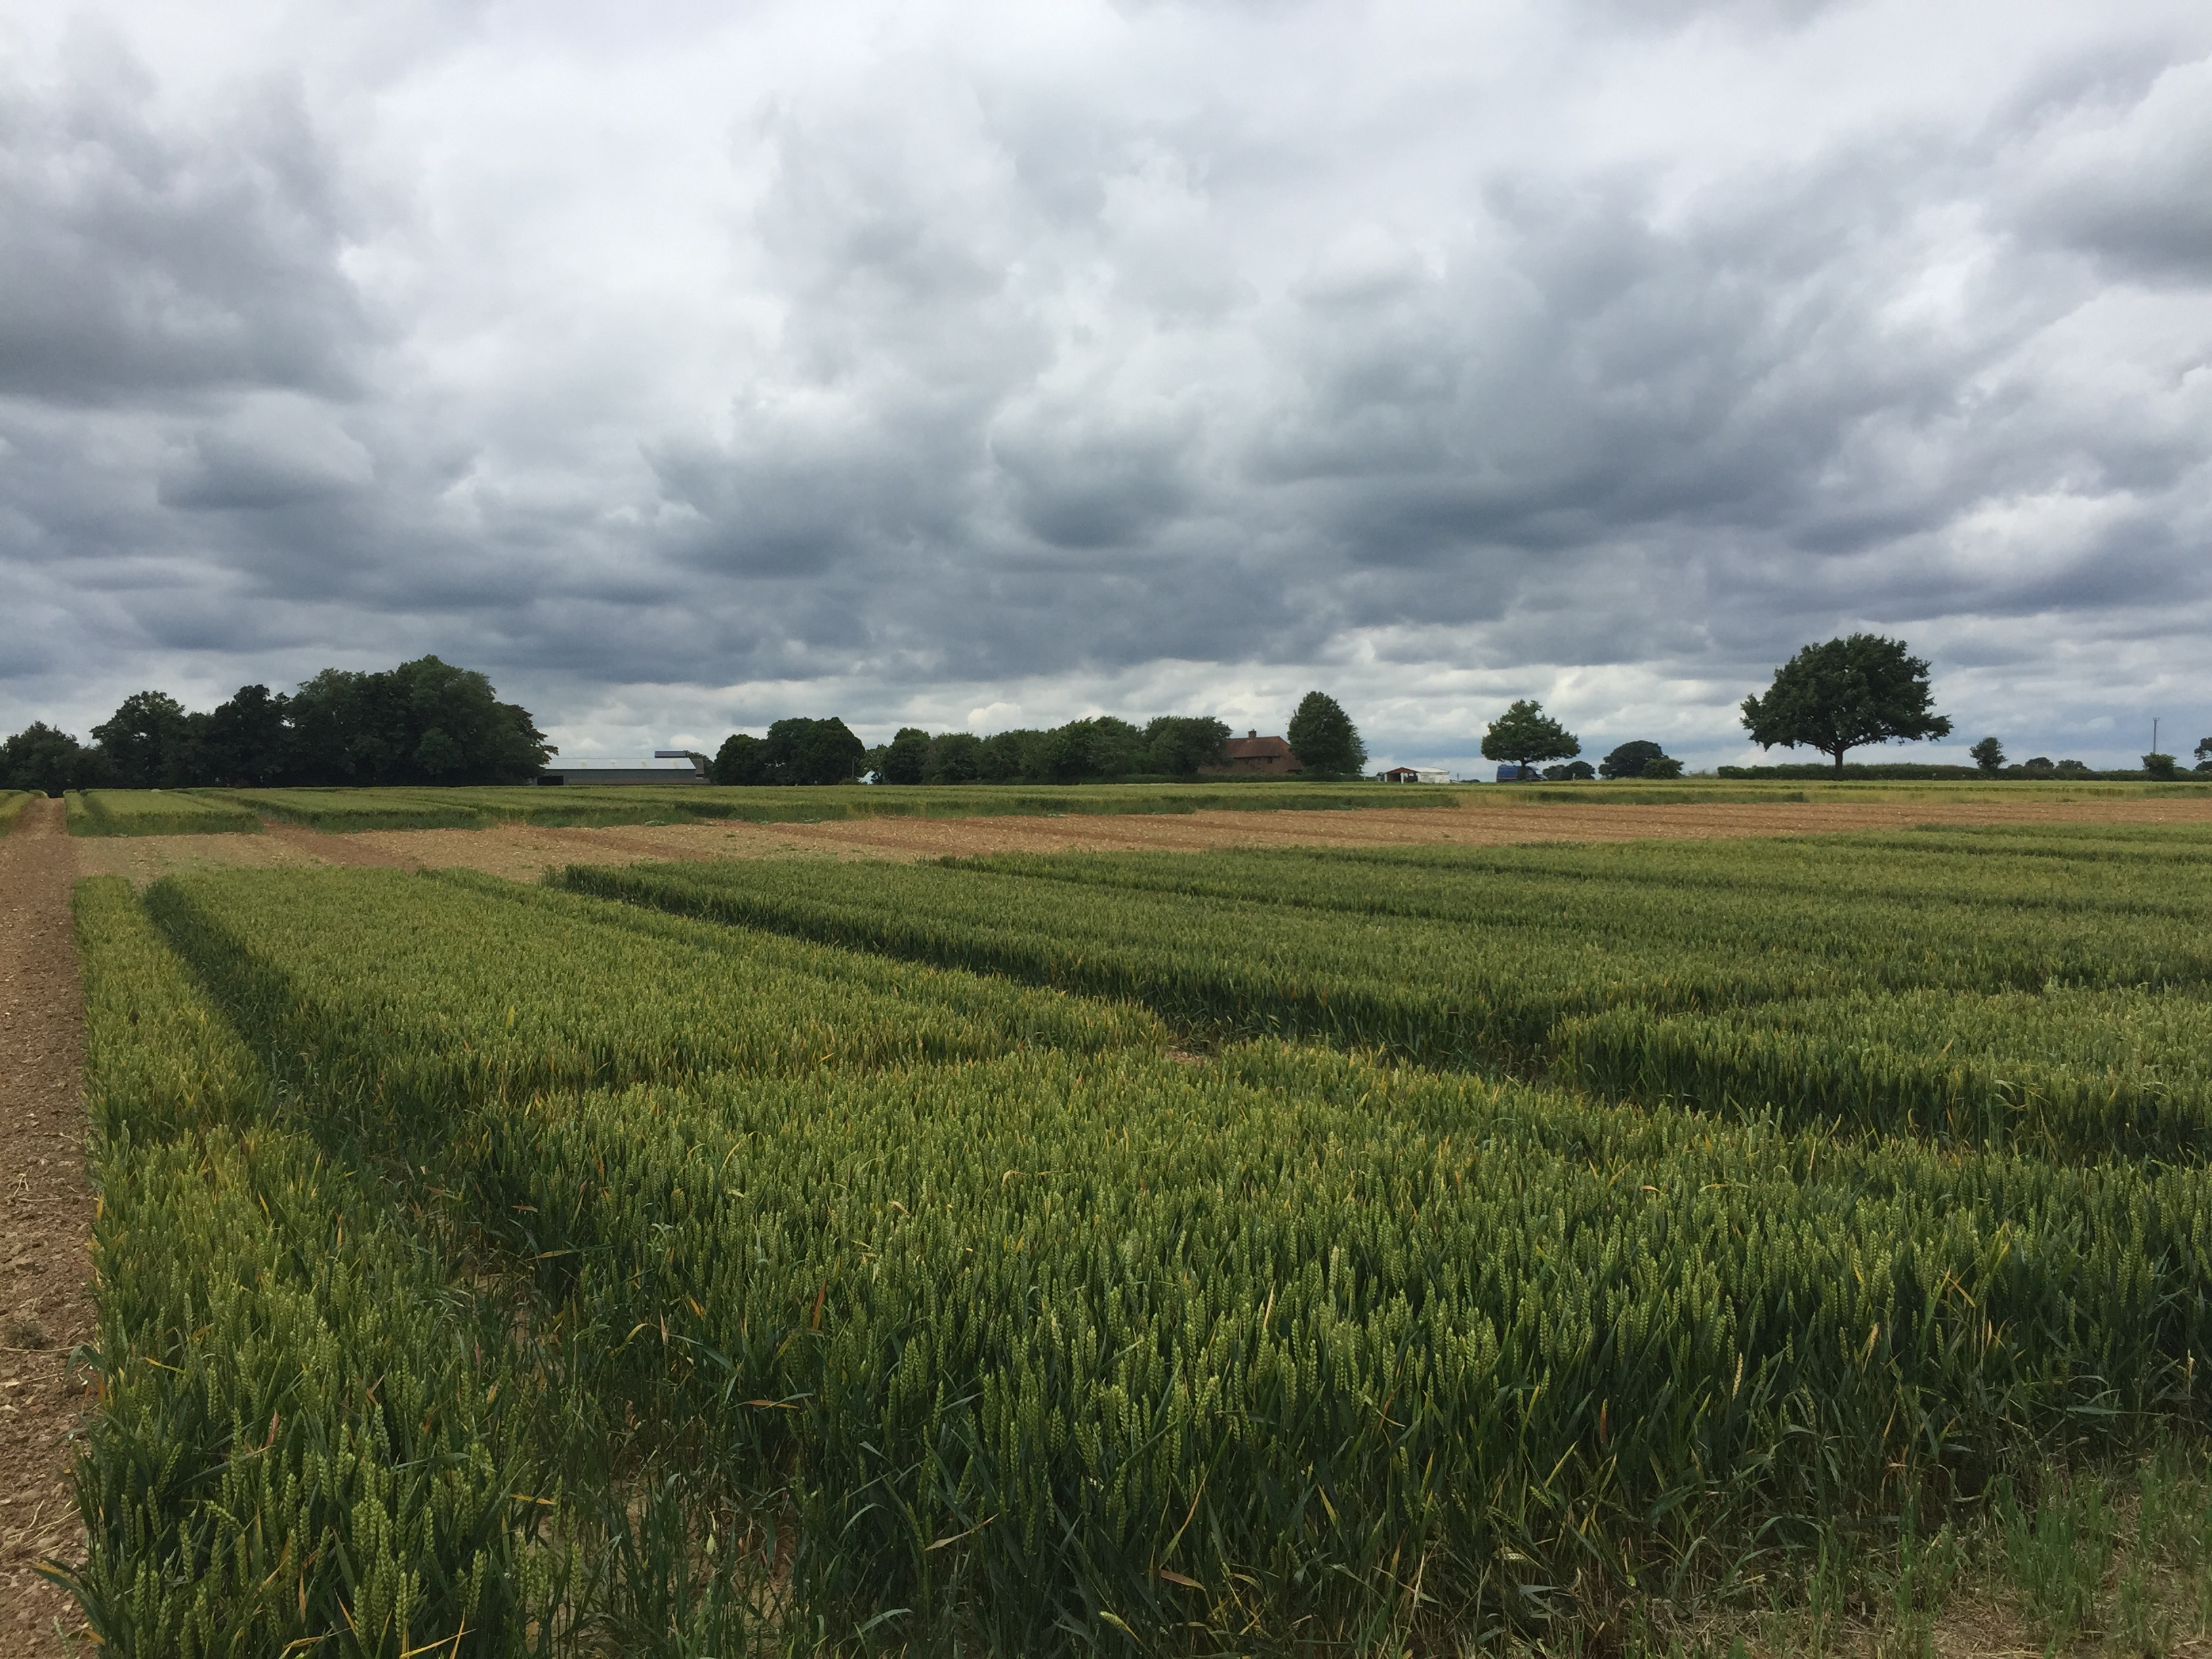
\includegraphics[width=0.75\linewidth]{figures/broadbalk} 
 
 }
 
 \caption{The Broadbalk experiment, Rothamsted (photograph taken 2016)}\label{fig:broadbalk}
 \end{figure}

\hypertarget{motivation}{%
\section{Motivation}\label{motivation}}

\begin{example}
\protect\hypertarget{exm:motivation}{}\label{exm:motivation}

Consider an experiment to compare two treatments (e.g.~drugs, diets, fertilisers, \(\dots\)). We have \(n\) subjects (people, mice, plots of land, \(\dots\)), each of which can be assigned one of the two treatments. A response (protein measurement, weight, yield, \(\dots\)) is then measured.

\end{example}

\textbf{Question:} How many subjects should be assigned to each treatment to gain the most precise\footnote{Smallest variance.} inference about the difference in response from the two treatments?

Consider a linear statistical model\footnote{In this course, we will almost always start with a statistical model which we wish to use to answer our scientific question.} for the response (see MATH2010 or MATH6174/STAT6123):

\begin{equation}
Y_j=\beta_{0}+\beta_{1}x_j+\varepsilon_j\,,\qquad j=1, \ldots, n\,,
\label{eq:slr}
\end{equation}

where \(\varepsilon_j\sim N(0,\sigma^{2})\) are independent and identically distributed errors and \(\beta_{0}, \beta_{1}\) are unknown constants (parameters).

Let\footnote{Other codings can be used: e.g. 0,1; see later in the module. It makes no difference for our current purpose.}
\begin{equation}
x_{j}=\left\{\begin{array}{ll}
-1&\textrm{if treatment 1 is applied to the $j$th subject}\\
+1&\textrm{if treatment 2 is applied to the $j$th subject}\nonumber ,
\end{array}
\right.
\end{equation}
for \(j=1,\dots,n\).\footnote{We will discuss the choice of \emph{coding} -1, +1 later.}

The difference in expected response from treatments 1 and 2 is

\begin{equation}
\begin{split}
\textrm{E}[Y_j\, |\, x_j = +1] - \textrm{E}[Y_j\, |\, x_j = -1] & = \beta_{0}+\beta_{1}-\beta_{0}+\beta_{1} \\
& = 2\beta_{1}\,.
\end{split}
\label{eq:ex-ex-response}
\end{equation}

Therefore, we require the the most precise estimator of \(\beta_{1}\) possible. That is, we wish to make the variance of our estimator of \(\beta_1\) as small as possible.

Parameters \(\beta_{0}\) and \(\beta_{1}\) can be estimated using least squares (see MATH2010 or MATH6174/STAT6123). For \(Y_1,\dots,Y_n\), we can write the model down in matrix form:

\begin{equation*}
\left[ \begin{array}{c}
Y_1\\
\vdots\\
Y_n\end{array}\right]
=\left[ \begin{array}{cc}
1&x_{1}\\
\vdots&\vdots\\
1&x_{n}\end{array}\right]
\left[ \begin{array}{c}
\beta_{0}\\
\beta_{1}\end{array}\right]
+\left[ \begin{array}{c}
\varepsilon_{1}\\
\vdots\\
\varepsilon_{n}\end{array}\right]\,.
\end{equation*}

Or, by defining some notation:

\begin{equation}
\boldsymbol{Y}=X\boldsymbol{\beta}+\boldsymbol{\varepsilon}\,
\label{eq:matrix-model}
\end{equation}

where

\begin{itemize}
\tightlist
\item
  \(\boldsymbol{Y}\) - \(n\times 1\) vector of responses;
\item
  \(X\) - \(n\times p\) model matrix;
\item
  \(\boldsymbol{\beta}\) - \(p\times 1\) vector of parameters;
\item
  \(\boldsymbol{\varepsilon}\) - \(n\times 1\) vector of errors.
\end{itemize}

The \textbf{least squares estimators}, \(\hat{\boldsymbol{\beta}}\), are chosen such that the quadratic form

\begin{equation*}
(\boldsymbol{Y}-X\boldsymbol{\beta})^{\textrm{T}}(\boldsymbol{Y}-X\boldsymbol{\beta})
\end{equation*}

is minimised (recall that \(\textrm{E}(\textbf{Y})=X\boldsymbol{\beta}\)). Therefore

\begin{equation*}
\hat{\boldsymbol{\beta}} = \textrm{argmin}_{\boldsymbol{\beta}}(\boldsymbol{Y}^{\textrm{T}}\boldsymbol{Y}+\boldsymbol{\beta}^{\textrm{T}}X^{\textrm{T}}X\boldsymbol{\beta}
-2\boldsymbol{\beta}^{\textrm{T}}X^{\textrm{T}}\boldsymbol{Y})\,.
\end{equation*}

If we differentiate with respect to \(\boldsymbol{\beta}\)\footnote{Check the \href{https://www.math.uwaterloo.ca/~hwolkowi/matrixcookbook.pdf}{Matrix Cookbook} for matrix calculus, amongst much else.},

\begin{equation*}
\frac{\partial}{\partial\boldsymbol{\beta}}=2X^{\textrm{T}}X\boldsymbol{\beta}-2X^{\textrm{T}}\boldsymbol{Y}\,,\nonumber
\end{equation*}

and equate to 0, we get the estimators

\begin{equation}
\hat{\boldsymbol{\beta}}=(X^{\textrm{T}}X)^{-1}X^{\textrm{T}}\boldsymbol{Y}\,.
\label{eq:lsestimators}
\end{equation}

These are the least squares estimators.

For Example \ref{exm:motivation},

\[
X=\left[\begin{array}{cc}
1&x_{1}\\
\vdots&\vdots\\
1&x_{n}\end{array}\right]\,,
\qquad
X^{\textrm{T}}X=\left[\begin{array}{cc}
n&\sum x_j\\
\sum x_j&\sum x_j^{2}\end{array}\right]\,,
\]

\[
(X^{\textrm{T}}X)^{-1}=\frac{1}{n\sum x_j^{2}-(\sum x_j)^{2}}\left[\begin{array}{cc}
\sum x_j^{2}&-\sum x_j\\
-\sum x_j&n\end{array}\right]\,,
\qquad
X^{\textrm{T}}\boldsymbol{Y}=\left[\begin{array}{c}
\sum Y_j\\
\sum x_jY_j\end{array}\right]\,.
\]
Then,
\begin{align}
\hat{\boldsymbol{\beta}}=\left[\begin{array}{c}
\hat{\beta}_{0}\\
\hat{\beta}_{1}\end{array}\right]
& =\frac{1}{n\sum x_j^{2}-(\sum x_j)^{2}}
\left[\begin{array}{cc}
\sum x_j^{2}&-\sum x_j\\
-\sum x_j&n\end{array}\right]
\left[\begin{array}{c}
\sum Y_j\\
\sum x_jY_j\end{array}\right]\nonumber \\
&= \frac{1}{n\sum x_j^{2}-(\sum x_j)^{2}}\left[\begin{array}{c}
\sum Y_j\sum x_j^{2}-\sum x_j\sum x_jY_j\\
n\sum x_jY_j-\sum x_j\sum Y_j\end{array}\right]\,.
\end{align}

We don't usually work through the algebra in such detail; the matrix form is often sufficient for theoretical and numerical calculations and software, e.g.~\texttt{R}, can be used.

The precision of \(\hat{\boldsymbol{\beta}}\) is measured via the variance-covariance matrix, given by
\begin{align}
\textrm{Var}(\hat{\boldsymbol{\beta}}) & = \textrm{Var}\{(X^{\textrm{T}}X)^{-1}X^{\textrm{T}}\boldsymbol{Y}\}\\
& =(X^{\textrm{T}}X)^{-1}X^{\textrm{T}}\textrm{Var}(\boldsymbol{Y})X(X^{\textrm{T}}X)^{-1}\\
& = (X^{\textrm{T}}X)^{-1}\sigma^{2}\,,
\end{align}

where \(\boldsymbol{Y}\sim N(X\boldsymbol{\beta},I_n\sigma^{2})\), where \(I_n\) is an \(n\times n\) identity matrix.

Hence, in our example,
\begin{align*}
\textrm{Var}(\hat{\boldsymbol{\beta}}) & = \frac{1}{n\sum x_j^{2}-(\sum x_j)^{2}}\left[\begin{array}{cc}
\sum x_j^{2}&-\sum x_j\\
-\sum x_j&n\end{array}\right]\sigma^{2}\\
& = \left[\begin{array}{cc}
\textrm{Var}(\hat\beta_{0})&\textrm{Cov}(\hat\beta_{0},\hat\beta_{1})\\
\textrm{Cov}(\hat\beta_{0},\hat\beta_{1})&\textrm{Var}(\hat\beta_{1})\end{array}\right]\,.
\end{align*}

For estimating the difference between treatments, we are interested in

\begin{align*}
\textrm{Var}(\hat{\beta}_{1})& = \frac{n}{n\sum x_j^{2}-(\sum x_j)^{2}}\sigma^{2}\\
 & = \frac{n}{n^2 - (\sum x_j)^2}\sigma^{2}\,,
\end{align*}
as \(x_j=\pm 1\), therefore \(x_j^2=1\) for all \(j=1,\ldots,n\), and hence \(\sum x_j^2=n\).

To achieve the most precise estimator, we need to minimise \(\textrm{Var}(\hat{\beta}_{1})\) or equivalently minimise \(|\sum x_j|\). This goal can be achieved through the choice of \(x_{1},\dots,x_{n}\):

\begin{itemize}
\tightlist
\item
  as each \(x_j\) can only take one of two values, -1 or +1, this is equivalent to choosing the numbers of subjects assigned to treatment 1 and treatment 2;
\item
  call these \(n_{1}\) and \(n_{2}\) respectively, with \(n_{1}+n_{2}=n\)
\end{itemize}

It is obvious that \(\sum x_j = 0\) if and only if \(n_1=n_2\). Therefore, assuming \(n\) is even, the \textbf{optimal design} has

\begin{itemize}
\tightlist
\item
  \(n_{1}=\frac{n}{2}\) subjects assigned to treatment 1 and
\item
  \(n_{2}=\frac{n}{2}\) subjects assigned to treatment 2.
\end{itemize}

For \(n\) odd, we choose \(n_{1}=\frac{n+1}{2}\), \(n_{2}=\frac{n-1}{2}\), or vice versa.

\begin{definition}
\protect\hypertarget{def:simple-efficiency}{}\label{def:simple-efficiency}

We can assess different designs using their \textbf{efficiency}:
\begin{equation}
\textrm{Eff}=\frac{\textrm{Var}(\hat{\beta}_{1}\, |\, d^{*})}{\textrm{Var}(\hat{\beta}_{1}\, |\, d_{1})}
\label{eq:simple-efficiency}
\end{equation}

where \(d_{1}\) is a design we want to assess and \(d^{*}\) is the optimal design with smallest variance. Note that \(0\leq\textrm{Eff}\leq 1\).

\end{definition}

In Figure \ref{fig:simple-efficiency} below, we plot this efficiency for Example \ref{exm:motivation}, using different choices of \(n_1\). The total number of runs is fixed at \(n = 100\), and the function \texttt{eff} calculates the efficiency from Definition \ref{def:simple-efficiency} for a design with \(n_1\) subjects assigned to treatment 1. Clearly, efficiency of 1 is achieved when \(n_1 = n_2\) (equal allocation of treatments 1 and 2). If \(n_1=0\) or \(n_1 = 1\), the efficiency is zero; we cannot estimate the difference between two treatments if we only allocate subjects to one of them.



\begin{Shaded}
\begin{Highlighting}[]
\NormalTok{n }\OtherTok{\textless{}{-}} \DecValTok{100} 
\NormalTok{eff }\OtherTok{\textless{}{-}} \ControlFlowTok{function}\NormalTok{(n1) }\DecValTok{1} \SpecialCharTok{{-}}\NormalTok{ ((}\DecValTok{2} \SpecialCharTok{*}\NormalTok{ n1 }\SpecialCharTok{{-}}\NormalTok{ n) }\SpecialCharTok{/}\NormalTok{ n)}\SpecialCharTok{\^{}}\DecValTok{2} 
\FunctionTok{curve}\NormalTok{(eff, }\AttributeTok{from =} \DecValTok{0}\NormalTok{, }\AttributeTok{to =}\NormalTok{ n, }\AttributeTok{ylab =} \StringTok{"Eff"}\NormalTok{, }\AttributeTok{xlab =} \FunctionTok{expression}\NormalTok{(n[}\DecValTok{1}\NormalTok{]))}
\end{Highlighting}
\end{Shaded}

\begin{figure}
\centering
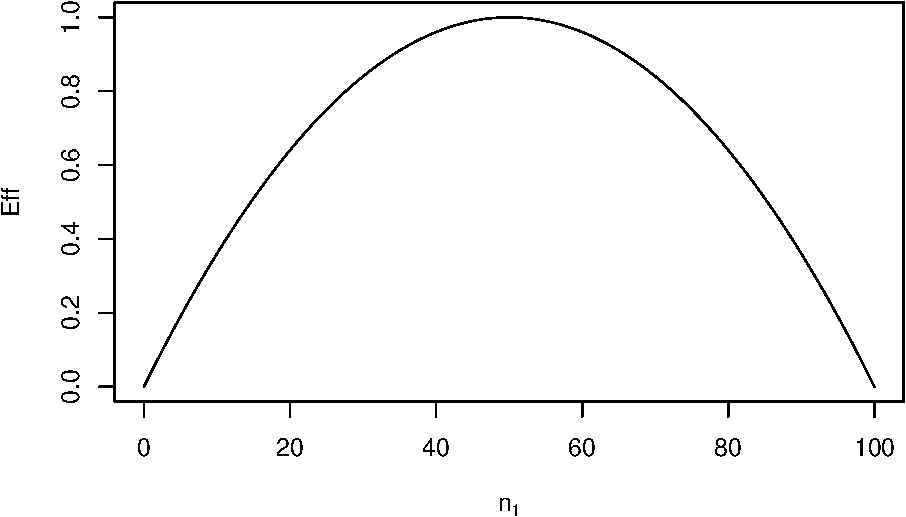
\includegraphics{bookdown_math3014-6027_files/figure-latex/simple-efficiency-1.pdf}
\caption{\label{fig:simple-efficiency}Efficiencies for designs for Example \ref{exm:motivation} with different numbers, \(n_1\), of subjects assigned to treatment 1 when the total number of subjects is \(n=100\).}
\end{figure}

\hypertarget{aims-of-experimentation-and-some-examples}{%
\section{Aims of experimentation and some examples}\label{aims-of-experimentation-and-some-examples}}

Some reasons experiments are performed:

\begin{enumerate}
\def\labelenumi{\arabic{enumi}.}
\tightlist
\item
  Treatment comparison (Chapters 2 and 3)
\end{enumerate}

\begin{itemize}
\tightlist
\item
  compare several treatments (and choose the best)
\item
  e.g.~clinical trial, agricultural field trial
\end{itemize}

\begin{enumerate}
\def\labelenumi{\arabic{enumi}.}
\setcounter{enumi}{1}
\tightlist
\item
  Factor screening (Chapters 4, 5 and 6)
\end{enumerate}

\begin{itemize}
\tightlist
\item
  many complex systems may involve a large number of (discrete) factors (controllable features)
\item
  which of these factors have a substantive impact?
\item
  (relatively) small experiments
\item
  e.g.~industrial experiments on manufacturing processes
\end{itemize}

\begin{enumerate}
\def\labelenumi{\arabic{enumi}.}
\setcounter{enumi}{2}
\tightlist
\item
  Response surface exploration (Chapter 7)
\end{enumerate}

\begin{itemize}
\tightlist
\item
  detailed description of relationship between important (continuous) variables and response
\item
  typically second order polynomial regression models
\item
  larger experiments, often built up sequentially
\item
  e.g.~alcohol yields in a pharmaceutical experiments
\end{itemize}

\begin{enumerate}
\def\labelenumi{\arabic{enumi}.}
\setcounter{enumi}{3}
\tightlist
\item
  Optimisation (Chapter 7)
\end{enumerate}

\begin{itemize}
\tightlist
\item
  finding settings of variables that lead to maximum or minimum response
\item
  typically use response surface methods and sequential ``hill climbing'\,' strategy
\end{itemize}

\hypertarget{some-definitions}{%
\section{Some definitions}\label{some-definitions}}

\begin{definition}
\protect\hypertarget{def:response}{}\label{def:response}

The \textbf{response} \(Y\) is the outcome measured in an experiment; e.g.~yield from a chemical process. The response from the \(n\) observations are denoted \(Y_{1},\dots,Y_{n}\).

\end{definition}

\begin{definition}
\protect\hypertarget{def:factor-variable}{}\label{def:factor-variable}

\textbf{Factors} (discrete) or \textbf{variables} (continuous) are features which can be set or controlled in an experiment; \(m\) denotes the number of factors or variables under investigation. For discrete factors, we call the possible settings of the factor its \textbf{levels}. We denote by \(x_{ij}\) the value taken by factor or variable \(i\) in the \(j\)th run of the experiment (\(i = 1, \ldots, m\); \(j = 1, \ldots, n\)).

\end{definition}

\begin{definition}
\protect\hypertarget{def:treatment}{}\label{def:treatment}

The \textbf{treatments} or \textbf{support points} are the \emph{distinct} combinations of factor or variable values in the experiment.

\end{definition}

\begin{definition}
\protect\hypertarget{def:unit}{}\label{def:unit}

An experimental \textbf{unit} is the basic element (material, animal, person, time unit, \ldots) to which a treatment can be applied to produce a response.

\end{definition}

In Example \ref{exm:motivation} (comparing two treatments):

\begin{itemize}
\tightlist
\item
  Response \(Y\): Measured outcome, e.g.~protein level or pain score in clinical trial, yield in an agricultural field trial.
\item
  Factor \(x\): ``treatment'' applied
\item
  Levels
  \[
  \begin{array}{ll}
  \textrm{treatment 1}&x =-1\\
  \textrm{treatment 2}&x =+1
  \end{array}
  \]
\item
  Treatment or support point: Two treatments or support points
\item
  Experimental unit: Subject (person, animal, plot of land, \ldots).
\end{itemize}

\hypertarget{principles}{%
\section{Principles of experimentation}\label{principles}}

Three fundamental principles that need to be considered when designing an experiment are:

\begin{itemize}
\tightlist
\item
  replication
\item
  randomisation
\item
  stratification (blocking)
\end{itemize}

\hypertarget{replication}{%
\subsection{Replication}\label{replication}}

Each treatment is applied to a number of experimental units, with the \(j\)th treatment replicated \(r_{j}\) times. This enables the estimation of the variances of treatment effect estimators; increasing the number of replications, or replicates, decreases the variance of estimators of treatment effects.
(Note: proper replication involves independent application of the treatment to different experimental units, not just taking several measurements from the same unit).

\hypertarget{randomisation}{%
\subsection{Randomisation}\label{randomisation}}

Randomisation should be applied to the allocation of treatments to units. Randomisation protects against \textbf{bias}; the effect of
variables that are unknown and potentially uncontrolled or
subjectivity in applying treatments. It also provides a formal basis
for inference and statistical testing.

For example, in a clinical trial to compare a new drug and a control random allocation protects against

\begin{itemize}
\tightlist
\item
  ``unmeasured and uncontrollable'' features (e.g.~age, sex, health)
\item
  bias resulting from the clinician giving new drug to patients who are sicker.
\end{itemize}

Clinical trials are usually also \emph{double-blinded}, i.e.~neither the healthcare professional nor the patient knows which treatment the patient is receiving.

\hypertarget{intro-blocking}{%
\subsection{Stratification (or blocking)}\label{intro-blocking}}

We would like to use a wide variety of experimental units (e.g.~people or plots of land) to ensure \textbf{coverage} of our results, i.e.~validity of our conclusions across the population of interest. However, if the sample of units from the population is too heterogenous, then this will induce too much random variability, i.e.~increase \(\sigma^{2}\) in \(\varepsilon_{j}\sim N(0,\sigma^{2})\), and hence increase the variance of our parameter estimators.

We can reduce this extraneous variation by splitting our units into homogenous sets, or \textbf{blocks}, and including a blocking term in the model. The simplest blocked experiment is a \textbf{randomised complete block design}, where each block contains enough units for all treatments to be applied. Comparisons can then be made \emph{within} each block.

Basic principle: block what you can, randomise what you cannot.

Later we will look at blocking in more detail, and the principle of \textbf{incomplete blocks}.

\hypertarget{lin-model-rev}{%
\section{Revision on the linear model}\label{lin-model-rev}}

Recall: \(\boldsymbol{Y}=X\boldsymbol{\beta}+\boldsymbol{\varepsilon}\), with \(\boldsymbol{\varepsilon}\sim N(\boldsymbol{0},I_n\sigma^{2})\). Let the \(j\)th row of \(X\) be denoted \(\boldsymbol{x}^\textrm{T}_j\), which holds the values of the predictors, or explanatory variables, for the \(j\)th observation. Then

\begin{equation*}
Y_j=\boldsymbol{x}_j^{\textrm{T}}\boldsymbol{\beta}+\varepsilon_j\,,\quad j=1,\ldots,n\,.
\end{equation*}

For example, quite commonly, for continuous variables

\[
\boldsymbol{x}_j=(1,x_{1j},x_{2j},\dots,x_{mj})^{\textrm{T}}\,,
\]

and so
\[
\boldsymbol{x}_j^{\textrm{T}}\boldsymbol{\beta}=\beta_{0}+\beta_{1}x_{1j}+\dots+\beta_{m}x_{mj}\,.
\]

The laest squares estimators are given by

\begin{equation}
\hat{\boldsymbol{\beta}}=(X^{\textrm{T}}X)^{-1}X^{\textrm{T}}\boldsymbol{Y}\,,\nonumber
\end{equation}

with

\begin{equation}
\textrm{Var}(\hat{\boldsymbol{\beta}})=(X^{\textrm{T}}X)^{-1}\sigma^{2}\,.\nonumber
\end{equation}

\hypertarget{variance-of-a-predictionfitted-value}{%
\subsection{Variance of a Prediction/Fitted Value}\label{variance-of-a-predictionfitted-value}}

A prediction of the mean response at point \(\boldsymbol{x}_0\) (which may or may not be in the design) is

\[
\hat{Y}_0 = \boldsymbol{x}_0^{\textrm{T}}\hat{\boldsymbol{\beta}}\,,
\]

with

\begin{align*}
\textrm{Var}(\hat{Y}_0) & = \textrm{Var}\left(\boldsymbol{x}_0^{\textrm{T}}\hat{\boldsymbol{\beta}}\right) \\
& = \boldsymbol{x}_0^{\textrm{T}}\textrm{Var}(\hat{\boldsymbol{\beta}})\boldsymbol{x}_0 \\
& = \boldsymbol{x}_0^{\textrm{T}}(X^{\textrm{T}}X)^{-1}\boldsymbol{x}_0\sigma^{2}\,.
\end{align*}

For a linear model, this variance depends only on the assumed regression model and the design (through \(X\)), the point at which prediction is to be made (\(\boldsymbol{x}_0\)) and the value of \(\sigma^2\); it does not depend on data \(\boldsymbol{Y}\) or parameters \(\boldsymbol{\beta}\).

Similarly, we can find the variance-covariance matrix of the fitted values:
\[
\textrm{Var}(\hat{Y})=\textrm{Var}(X\hat{\boldsymbol{\beta}})=X(X^{\textrm{T}}X)^{-1}X^{\textrm{T}}\sigma^{2}\,.
\]

\hypertarget{anova-revision}{%
\subsection{\texorpdfstring{Analysis of Variance and R\(^{2}\) as Model Comparison}{Analysis of Variance and R\^{}\{2\} as Model Comparison}}\label{anova-revision}}

To assess the goodness-of-fit of a model, we can use the residual sum of squares

\begin{align*}
\textrm{RSS} & = (\boldsymbol{Y} - X\hat{\boldsymbol{\beta}})^{\textrm{T}} (\boldsymbol{Y} - X\hat{\boldsymbol{\beta}})\\
& = \sum^{n}_{j=1}\left\{Y_{j}-\boldsymbol{x}_{j}^{\textrm{T}}\hat{\boldsymbol{\beta}}\right\}^{2}\\
& = \sum^{n}_{j=1}r_{j}^{2}\,,
\end{align*}

where

\[
r_{j}=Y_{j}-\boldsymbol{x}_{j}^{\textrm{T}}\hat{\boldsymbol{\beta}}\,.
\]

Often, a comparison is made to the null model

\[
Y_{j}=\beta_{0}+\varepsilon_{j}\,,
\]

i.e.~\(Y_{i}\sim N(\beta_{0},\sigma^{2})\). The residual sum of squares for the null model is given by

\[
\textrm{RSS}(\textrm{null}) = \boldsymbol{Y}^{\textrm{T}}\boldsymbol{Y} - m\bar{Y}^{2}\,,
\]
as

\[
\hat{\beta}_{0} = \bar{Y} = \frac{1}{n}\sum_{j=1}^n Y_{j}\,.
\]

How do we compare these models?

\begin{enumerate}
\def\labelenumi{\arabic{enumi}.}
\tightlist
\item
  Ratio of residual sum of squares:
  \begin{align*}
  R^{2} & = 1 - \frac{\textrm{RSS}}{\textrm{RSS}(\textrm{null})} \\
  & = 1 - \frac{(\boldsymbol{Y}-X\hat{\boldsymbol{\beta}})^{\textrm{T}}(\boldsymbol{Y}-X\hat{\boldsymbol{\beta}})}{\boldsymbol{Y}^{\textrm{T}}\boldsymbol{Y}-n\bar{Y}^{2}}\,.
  \end{align*}
\end{enumerate}

The quantity \(0\leq R^{2}\leq 1\) is sometimes called the \textbf{coefficient of multiple determination}:

\begin{itemize}
\tightlist
\item
  high \(R^{2}\) implies that the model describes much of the variation in the data;
\item
  \textbf{but} note that \(R^{2}\) will always increase as \(p\) (the number of explanatory variables) increases, with \(R^{2}=1\) when \(p=n\);
\item
  some software packages will report the adjusted \(R^{2}\).
\end{itemize}

\begin{align*}
R^{2}_{a} & = 1-\frac{\textrm{RSS}/(n-p)}{\textrm{RSS}(\textrm{null})/(n-1)}\\
& = 1 - \frac{(\boldsymbol{Y} - X\hat{\boldsymbol{\beta}})^{\textrm{T}} (\boldsymbol{Y} - X\hat{\boldsymbol{\beta}})/(n-p)}{(\boldsymbol{Y}^{\textrm{T}}\boldsymbol{Y} - n\bar{Y}^{2})/(n-1)};
\end{align*}

\begin{itemize}
\tightlist
\item
  \(R_a^2\) does not necessarily increase with \(p\) (as we divide by degrees of freedom to adjust for complexity of the model).
\end{itemize}

\begin{enumerate}
\def\labelenumi{\arabic{enumi}.}
\setcounter{enumi}{1}
\tightlist
\item
  Analysis of variance (ANOVA): An ANOVA table is compact way of presenting the results of (sequential) comparisons of nested models. You should be familiar with an ANOVA table of the following form.
\end{enumerate}

\begin{longtable}[]{@{}
  >{\raggedright\arraybackslash}p{(\columnwidth - 6\tabcolsep) * \real{0.25}}
  >{\raggedright\arraybackslash}p{(\columnwidth - 6\tabcolsep) * \real{0.25}}
  >{\raggedright\arraybackslash}p{(\columnwidth - 6\tabcolsep) * \real{0.25}}
  >{\raggedright\arraybackslash}p{(\columnwidth - 6\tabcolsep) * \real{0.25}}@{}}
\caption{\label{tab:anova} A standard ANOVA table.}\tabularnewline
\toprule
Source & Degress of Freedom & (Sequential) Sum of Squares & Mean Square \\
\midrule
\endfirsthead
\toprule
Source & Degress of Freedom & (Sequential) Sum of Squares & Mean Square \\
\midrule
\endhead
Regression & \(p-1\) & By subtraction; see \eqref{eq:SSS} & Reg SS/\((p-1)\) \\
Residual & \(n-p\) & \((\boldsymbol{Y}-X\hat{\boldsymbol{\beta}})^{\textrm{T}}(\boldsymbol{Y}-X\hat{\boldsymbol{\beta}})\)\footnote{Residual sum of squares for the full regression model.} & RSS/\((n-p)\) \\
Total & \(n-1\) & \(\boldsymbol{Y}^{\textrm{T}}\boldsymbol{Y}-n\bar{Y}^{2}\)\footnote{Residual sum of squares for the null model.} & \\
\bottomrule
\end{longtable}

In row 1 of Table \ref{tab:anova} above,
\begin{align}
\textrm{Regression SS = Total SS $-$ RSS} & = \boldsymbol{Y}^{\textrm{T}}\boldsymbol{Y} - n\bar{Y}^{2} - (\boldsymbol{Y}-X\hat{\boldsymbol{\beta}})^{\textrm{T}}(\boldsymbol{Y}-X\hat{\boldsymbol{\beta}})\\
& = -n\bar{Y}^{2}-\hat{\boldsymbol{\beta}}^{\textrm{T}}(X^{\textrm{T}}X)\hat{\boldsymbol{\beta}}+2\hat{\boldsymbol{\beta}}^{\textrm{T}}X^{\textrm{T}}\boldsymbol{Y} \\
& = \hat{\boldsymbol{\beta}}^{\textrm{T}}(X^{\textrm{T}}X)\hat{\boldsymbol{\beta}}-n\bar{Y}^{2}\,,
\label{eq:SSS}
\end{align}

with the last line following from
\begin{align*}
\hat{\boldsymbol{\beta}}^{\textrm{T}}X^{\textrm{T}}\boldsymbol{Y} & =
\hat{\boldsymbol{\beta}}^{\textrm{T}}(X^{\textrm{T}}X)(X^{\textrm{T}}X)^{-1}X^{\textrm{T}}\boldsymbol{Y} \\
& = \hat{\boldsymbol{\beta}}^{\textrm{T}}(X^{\textrm{T}}X)\hat{\boldsymbol{\beta}}
\end{align*}

This idea can be generalised to the comparison of a \emph{sequence} of nested models - see Problem Sheet 1.

Hypothesis testing is performed using the mean square:

\begin{equation}
\frac{\textrm{Regression SS}}{p-1}=\frac{\hat{\boldsymbol{\beta}}^{\textrm{T}}(X^{\textrm{T}}X)\hat{\boldsymbol{\beta}}-n\bar{Y}^{2}}{p-1}\,.\nonumber
\end{equation}

Under \(\textrm{H}_{0}: \beta_{1}=\dots=\beta_{p-1}=0\)

\begin{align*}
\frac{\textrm{Regression SS}/(p-1)}{\textrm{RSS}/(n-p)} & = \frac{(\hat{\boldsymbol{\beta}}^{\textrm{T}}(X^{\textrm{T}}X)\hat{\boldsymbol{\beta}} - n\bar{Y}^{2})/(p-1)}{(\boldsymbol{Y}-X\hat{\boldsymbol{\beta}})^{\textrm{T}}(\boldsymbol{Y}-X\hat{\boldsymbol{\beta}})/(n-p)}\nonumber\\
& \sim F_{p-1,n-p}\,,
\end{align*}

an \(F\) distribution with \(p-1\) and \(n-p\) degrees of freedom; defined via the ratio of two independent \(\chi^{2}\) distributions.

Also,

\begin{equation*}
\frac{\textrm{RSS}}{n-p}=\frac{(\boldsymbol{Y}-X\hat{\boldsymbol{\beta}})^{\textrm{T}}(\boldsymbol{Y}-X\hat{\boldsymbol{\beta}})}{n-p}=\hat{\sigma}^{2}
\end{equation*}

is an unbiased estimator for \(\sigma^{2}\), and

\begin{equation*}
\frac{(n-p)}{\sigma^{2}}\hat{\sigma}^{2}\sim\chi^{2}_{n-p}\,.
\end{equation*}

This is a Chi-squared distribution with \(n-p\) degrees of freedom (see MATH2010 or MATH6174 notes).

\hypertarget{exercises}{%
\section{Exercises}\label{exercises}}

\begin{enumerate}
\def\labelenumi{\arabic{enumi}.}
\item
  \citep[Adapted from][]{Morris2011} A classic and famous example of a simple hypothetical experiment was described by \citet{Fisher1935}:

  \begin{quote}
  A lady declares that by tasting a cup of tea made with milk she can discriminate whether the milk or the tea infusion was added first to the cup. We will consider the problem of designing an experiment by means of which this assertion can be tested. For this purpose let us first lay down a simple form of experiment with a view to studying its limitations and its characteristics, both those that same essential to the experimental method, when well developed, and those that are not essential but auxiliary.

  Our experiment consists in mixing eight cups of tea, four in one way and four in the other, and presenting them to the subject for judgement in a random order. The subject has been told in advance of what the test will consist, namely that she will be asked to taste eight cups, that these shall be four of each kind, and that they shall be presented to her in a random order, that is an order not determined arbitrarily by human choice, but by the actual manipulation of the physical appartatus used in games of chance, cards, dice, roulettes, etc., or, more expeditiously, from a published collection of random sampling numbers purporting to give the actual results of such manipulation\footnote{Now, we would use routines such as \texttt{sample} in \texttt{R}.}. Her task is to divide the 8 cups into two sets of 4, agreeing, if possible, with the treatments received.
  \end{quote}

  \begin{enumerate}
  \def\labelenumii{\alph{enumii}.}
  \tightlist
  \item
    Define the treatments in this experiment.
  \item
    Identify the units in this experiment.
  \item
    How might a ``physical appartatus'' from a ``game of chance'' be used to perform the randomisation. Explain one example.
  \item
    Suppose eight tea cups are available for this experiment but they are not identical. Instead they come from two sets. Foru are made from heavy, thick porcelain; four from much lighter china. If each cup can only be used once, how might this fact be incorporated into the design of the experiment?
  \end{enumerate}
\end{enumerate}

Solution

\begin{enumerate}
\def\labelenumi{\alph{enumi}.}
\item
  There are two treatments in the experiment - the two ingredients ``milk first'' and ``tea first''.
\item
  The experimental units are the ``cups of tea'', made up from the tea and milk used and also the cup itself.
\item
  The simplest method here might be to select four black playing cards and four red playing cards, assign one treatment to each colour, shuffle the cards, and then draw them in order. The colour drawn indicates the treatment that should be used to make the next cup of tea. This operation would give one possible randomisation.

  We could of course also use \texttt{R}.

\begin{Shaded}
\begin{Highlighting}[]
\FunctionTok{sample}\NormalTok{(}\FunctionTok{rep}\NormalTok{(}\FunctionTok{c}\NormalTok{(}\StringTok{"Milk first"}\NormalTok{, }\StringTok{"Tea first"}\NormalTok{), }\FunctionTok{c}\NormalTok{(}\DecValTok{4}\NormalTok{, }\DecValTok{4}\NormalTok{)), }\AttributeTok{size =} \DecValTok{8}\NormalTok{, }\AttributeTok{replace =}\NormalTok{ F)}
\end{Highlighting}
\end{Shaded}

\begin{verbatim}
## [1] "Tea first"  "Milk first" "Milk first" "Tea first"  "Milk first"
## [6] "Tea first"  "Milk first" "Tea first"
\end{verbatim}
\item
  Type of cup could be considered as a blocking factor. One way of incorporating it would be to split the experiment into two (blocks), each with four cups (two milk first, two tea first). We would still wish to randomise allocation of treatments to units within blocks.

\begin{Shaded}
\begin{Highlighting}[]
\CommentTok{\# block 1}
\FunctionTok{sample}\NormalTok{(}\FunctionTok{rep}\NormalTok{(}\FunctionTok{c}\NormalTok{(}\StringTok{"Milk first"}\NormalTok{, }\StringTok{"Tea first"}\NormalTok{), }\FunctionTok{c}\NormalTok{(}\DecValTok{2}\NormalTok{, }\DecValTok{2}\NormalTok{)), }\AttributeTok{size =} \DecValTok{4}\NormalTok{, }\AttributeTok{replace =}\NormalTok{ F)}
\end{Highlighting}
\end{Shaded}

\begin{verbatim}
## [1] "Milk first" "Tea first"  "Milk first" "Tea first"
\end{verbatim}

\begin{Shaded}
\begin{Highlighting}[]
\CommentTok{\# block 2}
\FunctionTok{sample}\NormalTok{(}\FunctionTok{rep}\NormalTok{(}\FunctionTok{c}\NormalTok{(}\StringTok{"Milk first"}\NormalTok{, }\StringTok{"Tea first"}\NormalTok{), }\FunctionTok{c}\NormalTok{(}\DecValTok{2}\NormalTok{, }\DecValTok{2}\NormalTok{)), }\AttributeTok{size =} \DecValTok{4}\NormalTok{, }\AttributeTok{replace =}\NormalTok{ F)}
\end{Highlighting}
\end{Shaded}

\begin{verbatim}
## [1] "Milk first" "Tea first"  "Tea first"  "Milk first"
\end{verbatim}
\end{enumerate}

\begin{enumerate}
\def\labelenumi{\arabic{enumi}.}
\setcounter{enumi}{1}
\item
  Consider the linear model

  \[\boldsymbol{y}= X\boldsymbol{\beta}+ \boldsymbol{\varepsilon}\,,\]
  with \(\boldsymbol{y}\) an \(n\times 1\) vector of responses, \(X\) a \(n\times p\) model matrix and \(\boldsymbol{\varepsilon}\) a \(n\times 1\) vector of independent and identically distributed random variables with constant variance \(\sigma^2\).

  \begin{enumerate}
  \def\labelenumii{\alph{enumii}.}
  \tightlist
  \item
    Derive the least squares estimator \(\hat{\boldsymbol{\beta}}\) for this multiple linear regression model, and show that this estimator is unbiased. Using the definition of (co)variance, show that
  \end{enumerate}

  \[\mbox{Var}(\hat{\boldsymbol{\beta}}) = \left(X^{\mathrm{T}}X\right)^{-1}\sigma^2\,.\]

  \begin{enumerate}
  \def\labelenumii{\alph{enumii}.}
  \setcounter{enumii}{1}
  \tightlist
  \item
    If \(\boldsymbol{\varepsilon}\sim N (\boldsymbol{0},I_n\sigma^2)\), with \(I_n\) being the \(n\times n\) identity matrix, show that the maximum likelihood estimators for \(\boldsymbol{\beta}\) coincide with the least squares estimators.
  \end{enumerate}
\end{enumerate}

Solution

\begin{enumerate}
\def\labelenumi{\alph{enumi}.}
\item
  The method of least squares minimises the sum of squared differences between the responses and the expected values, that is, minimises the expression

  \[
   (\boldsymbol{y}-X\boldsymbol{\beta})^{\mathrm{T}}(\boldsymbol{y}-X\boldsymbol{\beta}) = \boldsymbol{y}^{\mathrm{T}}\boldsymbol{y}- 2\boldsymbol{\beta}^{\mathrm{T}}X^{\mathrm{T}}\boldsymbol{y}+ \boldsymbol{\beta}^{\mathrm{T}}X^{\mathrm{T}}X\boldsymbol{\beta}\,.
   \]
  Differentiating with respect to the vector \(\boldsymbol{\beta}\), we obtain

  \[
   \frac{\partial}{\partial\boldsymbol{\beta}} = -2X^{\mathrm{T}}\boldsymbol{y}+ 2X^{\mathrm{T}}X\boldsymbol{\beta}\,.
   \]

  Set equal to \(\boldsymbol{0}\) and solve:

  \[
   X^{\mathrm{T}}X\hat{\boldsymbol{\beta}} = X^{\mathrm{T}}\boldsymbol{y}\Rightarrow \hat{\boldsymbol{\beta}} = \left(X^{\mathrm{T}}X\right)^{-1}X^{\mathrm{T}}\boldsymbol{y}\,.
   \]

  The estimator \(\hat{\boldsymbol{\beta}}\) is unbiased:

  \[
   E(\hat{\boldsymbol{\beta}}) = \left(X^{\mathrm{T}}X\right)^{-1}X^{\mathrm{T}}E(\boldsymbol{y}) = \left(X^{\mathrm{T}}X\right)^{-1}X^{\mathrm{T}}X\boldsymbol{\beta}= \boldsymbol{\beta}\,,
   \]

  and has variance:

  \begin{align*}
  \mbox{Var}(\hat{\boldsymbol{\beta}}) & =E\left\{ \left[\hat{\boldsymbol{\beta}} - E(\hat{\boldsymbol{\beta}})\right] \left[\hat{\boldsymbol{\beta}} - E(\hat{\boldsymbol{\beta}})\right]^{\mathrm{T}} \right\}\\
   & =  E\left\{ \left[\hat{\boldsymbol{\beta}} - \boldsymbol{\beta}\right] \left[\hat{\boldsymbol{\beta}} - \boldsymbol{\beta}\right]^{\mathrm{T}} \right\}\\
   & = E\left\{ \hat{\boldsymbol{\beta}}\hat{\boldsymbol{\beta}}^{\mathrm{T}} - 2\boldsymbol{\beta}\hat{\boldsymbol{\beta}}^{\mathrm{T}} + \boldsymbol{\beta}\boldsymbol{\beta}^{\mathrm{T}} \right\}\\
   & = E\left\{ \left(X^{\mathrm{T}}X\right)^{-1}X^{\mathrm{T}}\boldsymbol{y}\boldsymbol{y}^{\mathrm{T}}X\left(X^{\mathrm{T}}X\right)^{-1}  - 2\boldsymbol{\beta}\boldsymbol{y}^{\mathrm{T}}X\left(X^{\mathrm{T}}X\right)^{-1} + \boldsymbol{\beta}\boldsymbol{\beta}^{\mathrm{T}}\right\}\\
   & = \left(X^{\mathrm{T}}X\right)^{-1}X^{\mathrm{T}}E(\boldsymbol{y}\boldsymbol{y}^{\mathrm{T}})X\left(X^{\mathrm{T}}X\right)^{-1} - 2\boldsymbol{\beta}E(\boldsymbol{y}^{\mathrm{T}})X\left(X^{\mathrm{T}}X\right)^{-1} + \boldsymbol{\beta}\boldsymbol{\beta}^{\mathrm{T}}\\
   & = \left(X^{\mathrm{T}}X\right)^{-1}X^{\mathrm{T}}\left[\mbox{Var}(\boldsymbol{y}) + E(\boldsymbol{y})E(\boldsymbol{y}^{\mathrm{T}})\right]X\left(X^{\mathrm{T}}X\right)^{-1} - 2\boldsymbol{\beta}\boldsymbol{\beta}^{\mathrm{T}}X^{\mathrm{T}}X\left(X^{\mathrm{T}}X\right)^{-1} + \boldsymbol{\beta}\boldsymbol{\beta}^{\mathrm{T}}\\
   & = \left(X^{\mathrm{T}}X\right)^{-1}X^{\mathrm{T}}\left[I_N\sigma^2 + X\boldsymbol{\beta}\boldsymbol{\beta}^{\mathrm{T}}X^{\mathrm{T}}\right]X\left(X^{\mathrm{T}}X\right)^{-1} - \boldsymbol{\beta}\boldsymbol{\beta}^{\mathrm{T}}\\
   & = \left(X^{\mathrm{T}}X\right)^{-1}\sigma^2\,. 
   \end{align*}
\item
  As \(\boldsymbol{y}\sim N\left(X\boldsymbol{\beta}, I_N\sigma^2\right)\), the likelihood is given by

  \[
   L(\boldsymbol{\beta}\,; \boldsymbol{y}) = \left(2\pi\sigma^2\right)^{-N/2}\exp\left\{-\frac{1}{2\sigma^2}(\boldsymbol{y}- X\boldsymbol{\beta})^{\mathrm{T}}(\boldsymbol{y}- X\boldsymbol{\beta})\right\}\,.
   \]

  The log-likelihood is given by

  \[
   l(\boldsymbol{\beta}\,;\boldsymbol{y}) = -\frac{1}{2\sigma^2}(\boldsymbol{y}- X\boldsymbol{\beta})^{\mathrm{T}}(\boldsymbol{y}- X\boldsymbol{\beta}) + \mbox{constant}\,.
   \]

  Up to a constant, this expression is \(-1\times\) the least squares equations; hence maximising the log-likelihood is equivalent to minimising the least squares equation.
\end{enumerate}

\begin{enumerate}
\def\labelenumi{\arabic{enumi}.}
\setcounter{enumi}{2}
\item
  Consider the two nested linear models

  \begin{enumerate}
  \def\labelenumii{(\roman{enumii})}
  \item
    \(Y_j = \beta_0 + \beta_1x_{1j} + \beta_2x_{2j} + \ldots + \beta_{p_1}x_{p_1j} + \varepsilon_j\), or \(\boldsymbol{y}= X_1\boldsymbol{\beta}_1 + \boldsymbol{\varepsilon}\),
  \item
    \(Y_j = \beta_0 + \beta_1x_{1j} + \beta_2x_{2j} + \ldots + \beta_{p_1}x_{p_1j} + \beta_{p_1+1}x_{(p_1+1)j} + \ldots + \beta_{p_2}x_{p_2j} + \varepsilon_j\), or \(\boldsymbol{y}= X_1\boldsymbol{\beta}_1 + X_2\boldsymbol{\beta}_2+ \boldsymbol{\varepsilon}\)
  \end{enumerate}

  with \(\varepsilon_j\sim N(0, \sigma^2)\), and \(\varepsilon_{j}\), \(\varepsilon_{k}\) independent \((\boldsymbol{\varepsilon}\sim N(\boldsymbol{0},I_n\sigma^2))\).

  \begin{enumerate}
  \def\labelenumii{\alph{enumii}.}
  \item
    Construct an ANOVA table to compare model (ii) with the null model \(Y_j=\beta_0 + \varepsilon_j\).
  \item
    Extend this ANOVA table to compare models (i) and (ii) by further decomposing the regression sum of squares for model (ii).
  \end{enumerate}

  \textbf{Hint:} which residual sum of squares are you interested in to compare models (i) and (ii)?

  You should end up with an ANOVA table of the form

  \begin{longtable}[]{@{}lccc@{}}
  \toprule
  Source & Degrees of freedom & Sums of squares & Mean square \\
  \midrule
  \endhead
  Model (i) & \(p_1\) & ? & ? \\
  Model (ii) & \(p_2\) & ? & ? \\
  Residual & \(n-p_1-p_2-1\) & ? & ? \\
  Total & \(n-1\) & \(\boldsymbol{y}^{\mathrm{T}}\boldsymbol{y}- n\bar{Y}^2\) & \\
  \bottomrule
  \end{longtable}

  The second row of the table gives the \textbf{extra sums of squares} for the additional terms in fitting model (ii), over and above those in model (i).

  \begin{enumerate}
  \def\labelenumii{\alph{enumii}.}
  \setcounter{enumii}{2}
  \tightlist
  \item
    Calculate the extra sum of squares for fitting the terms in model (i), over and above those terms only in model (ii), i.e.~those held in \(X_2\boldsymbol{\beta}_2\). Construct an ANOVA table containing both the extra sum of squares for the terms only in model (i) and the extra sum of squares for the terms only in model (ii). Comment on the table.
  \end{enumerate}
\end{enumerate}

Solution

\begin{enumerate}
\def\labelenumi{\alph{enumi}.}
\item
  From lectures

  \begin{longtable}[]{@{}
    >{\raggedright\arraybackslash}p{(\columnwidth - 6\tabcolsep) * \real{0.12}}
    >{\centering\arraybackslash}p{(\columnwidth - 6\tabcolsep) * \real{0.36}}
    >{\centering\arraybackslash}p{(\columnwidth - 6\tabcolsep) * \real{0.30}}
    >{\centering\arraybackslash}p{(\columnwidth - 6\tabcolsep) * \real{0.22}}@{}}
  \toprule
  Source & Degrees of freedom & Sums of squares & Mean square \\
  \midrule
  \endhead
  Regression & \(p_1+p_2\) & \(\hat{\boldsymbol{\beta}}^{\mathrm{T}}X^{\mathrm{T}}X\hat{\boldsymbol{\beta}} - n\bar{Y}^2\) & \(\left(\hat{\boldsymbol{\beta}}^{\mathrm{T}}X^{\mathrm{T}}X\hat{\boldsymbol{\beta}} - n\bar{Y}^2\right)/(p_1+p_2)\) \\
  Residual & \(n-p_1-p_2-1\) & \((\boldsymbol{y}- X\hat{\boldsymbol{\beta}})^{\mathrm{T}}(\boldsymbol{y}- X\hat{\boldsymbol{\beta}})\) & RSS\(/(n-p_1-p_2-1)\) \\
  Total & \(n-1\) & \(\boldsymbol{y}^{\mathrm{T}}\boldsymbol{y}- n\bar{Y}^2\) & \\
  \bottomrule
  \end{longtable}

  where

  \begin{align*}
  \mbox{RSS(null) - RSS(ii)} & = \boldsymbol{y}^{\mathrm{T}}\boldsymbol{y}- n\bar{Y}^2 - (\boldsymbol{y}- X\hat{\boldsymbol{\beta}})^{\mathrm{T}}(\boldsymbol{y}- X\hat{\boldsymbol{\beta}})\\
  & = \boldsymbol{y}^{\mathrm{T}}\boldsymbol{y}- n\bar{Y}^2 - \boldsymbol{y}^{\mathrm{T}}\boldsymbol{y}+ 2\boldsymbol{y}^{\mathrm{T}}X\hat{\boldsymbol{\beta}} - \hat{\boldsymbol{\beta}}^{\mathrm{T}}X^{\mathrm{T}}X\hat{\boldsymbol{\beta}}\\
  & = 2\hat{\boldsymbol{\beta}}^{\mathrm{T}}X^{\mathrm{T}}X\hat{\boldsymbol{\beta}} - \hat{\boldsymbol{\beta}}^{\mathrm{T}}X^{\mathrm{T}}X\hat{\boldsymbol{\beta}} - n\bar{Y}^2\\
  & = \hat{\boldsymbol{\beta}}^{\mathrm{T}}X^{\mathrm{T}}X\hat{\boldsymbol{\beta}} - n\bar{Y}^2\,.
   \end{align*}
\item
  To compare model (i) with the null model, we compute

  \begin{align*}
   \mbox{RSS(null) - RSS(i)} & = \boldsymbol{y}^{\mathrm{T}}\boldsymbol{y}- N\bar{Y}^2 - (\boldsymbol{y}- X_1\hat{\boldsymbol{\beta}}_1)^{\mathrm{T}}(\boldsymbol{y}- X_1\hat{\boldsymbol{\beta}}_1)\\
   & = \hat{\boldsymbol{\beta}}_1^{\mathrm{T}}X_1^{\mathrm{T}}X_1\hat{\boldsymbol{\beta}}_1 - n\bar{Y}^2\,.
   \end{align*}

  To compare models (i) and (ii), we compare them both to the null model, and look at the difference between these comparisons:

  \begin{align*}
   \mbox{[RSS(null) - RSS(ii)] - [RSS(null) - RSS(i)]} & = \mbox{RSS(i) - RSS(ii)}\\
   & = (\boldsymbol{y}- X_1\hat{\boldsymbol{\beta}}_1)^{\mathrm{T}}(\boldsymbol{y}- X_1\hat{\boldsymbol{\beta}}_1) - (\boldsymbol{y}- X\hat{\boldsymbol{\beta}})^{\mathrm{T}}(\boldsymbol{y}- X\hat{\boldsymbol{\beta}})\\
   & = \hat{\boldsymbol{\beta}}^{\mathrm{T}}X^{\mathrm{T}}X\hat{\boldsymbol{\beta}} - \hat{\boldsymbol{\beta}}_1^{\mathrm{T}}X_1^{\mathrm{T}}X_1\hat{\boldsymbol{\beta}}_1\,.
   \end{align*}

  \begin{longtable}[]{@{}
    >{\raggedright\arraybackslash}p{(\columnwidth - 6\tabcolsep) * \real{0.12}}
    >{\centering\arraybackslash}p{(\columnwidth - 6\tabcolsep) * \real{0.36}}
    >{\centering\arraybackslash}p{(\columnwidth - 6\tabcolsep) * \real{0.30}}
    >{\centering\arraybackslash}p{(\columnwidth - 6\tabcolsep) * \real{0.22}}@{}}
  \toprule
  Source & Degrees of freedom & Sums of squares & Mean square \\
  \midrule
  \endhead
  Regression & \(p_1+p_2\) & \(\hat{\boldsymbol{\beta}}X^{\mathrm{T}}X\hat{\boldsymbol{\beta}} - n\bar{Y}^2\) & \(\left(\hat{\boldsymbol{\beta}}X^{\mathrm{T}}X\hat{\boldsymbol{\beta}} - n\bar{Y}^2\right)/(p_1+p_2)\) \\
  Model (i) & \(p_1\) & \(\hat{\boldsymbol{\beta}}_1^{\mathrm{T}}X_1^{\mathrm{T}}X_1\hat{\boldsymbol{\beta}}_1 - n\bar{Y}^2\) & \(\left(\hat{\boldsymbol{\beta}}_1^{\mathrm{T}}X_1^{\mathrm{T}}X_1\hat{\boldsymbol{\beta}}_1 - n\bar{Y}^2\right)/p_1\) \\
  Extra due to Model (ii) & \(p_2\) & \(\hat{\boldsymbol{\beta}}^{\mathrm{T}}X^{\mathrm{T}}X\hat{\boldsymbol{\beta}} - \hat{\boldsymbol{\beta}}_1^{\mathrm{T}}X_1^{\mathrm{T}}X_1\hat{\boldsymbol{\beta}}_1\) & \(\left(\hat{\boldsymbol{\beta}}^{\mathrm{T}}X^{\mathrm{T}}X\hat{\boldsymbol{\beta}} - \hat{\boldsymbol{\beta}}_1^{\mathrm{T}}X_1^{\mathrm{T}}X_1\hat{\boldsymbol{\beta}}_1\right)/p_2\) \\
  Residual & \(n-p_1-p_2-1\) & \((\boldsymbol{y}- X\hat{\boldsymbol{\beta}})^{\mathrm{T}}(\boldsymbol{y}- X\hat{\boldsymbol{\beta}})\) & RSS\(/(n-p_1-p_2-1)\) \\
  Total & \(n-1\) & \(\boldsymbol{y}^{\mathrm{T}}\boldsymbol{y}- n\bar{Y}^2\) & \\
  \bottomrule
  \end{longtable}
\end{enumerate}

By definition, the Model (i) SS and the Extra SS for Model (ii) sum to the Regression SS.

\begin{enumerate}
\def\labelenumi{\alph{enumi}.}
\item
  The extra sum of squares for the terms in model (i) over and above those in model (ii) are obtained through comparison of the models

  ia. \(\boldsymbol{y}= X_2\boldsymbol{\beta}_2 + \boldsymbol{\varepsilon}\),

  iia. \(\boldsymbol{y}= X_1\boldsymbol{\beta}_1 + X_2\boldsymbol{\beta}_2+ \boldsymbol{\varepsilon}= X\boldsymbol{\beta}+ \varepsilon\)

  Extra sum of squares for model (iia):

  \begin{align*}
  \mbox{[RSS(null) - RSS(iia)] - [RSS(null) - RSS(ia)]} & = \mbox{RSS(ia) - RSS(iia)}\\
  & = (\boldsymbol{y}- X_2\hat{\boldsymbol{\beta}}_2)^{\mathrm{T}}(\boldsymbol{y}- X_2\hat{\boldsymbol{\beta}}_2) - (\boldsymbol{y}- X\hat{\boldsymbol{\beta}})^{\mathrm{T}}(\boldsymbol{y}- X\hat{\boldsymbol{\beta}})\\
  & = \hat{\boldsymbol{\beta}}^{\mathrm{T}}X^{\mathrm{T}}X\hat{\boldsymbol{\beta}} - \hat{\boldsymbol{\beta}}_2^{\mathrm{T}}X_2^{\mathrm{T}}X_2\hat{\boldsymbol{\beta}}_2\,.
   \end{align*}

  Hence, an ANOVA table for the extra sums of squares is given by

  \begin{longtable}[]{@{}
    >{\centering\arraybackslash}p{(\columnwidth - 6\tabcolsep) * \real{0.12}}
    >{\centering\arraybackslash}p{(\columnwidth - 6\tabcolsep) * \real{0.36}}
    >{\centering\arraybackslash}p{(\columnwidth - 6\tabcolsep) * \real{0.30}}
    >{\centering\arraybackslash}p{(\columnwidth - 6\tabcolsep) * \real{0.22}}@{}}
  \toprule
  Source & Degrees of freedom & Sums of squares & Mean square \\
  \midrule
  \endhead
  Regression & \(p_1+p_2\) & \(\hat{\boldsymbol{\beta}}X^{\mathrm{T}}X\hat{\boldsymbol{\beta}} - n\bar{Y}^2\) & \(\left(\hat{\boldsymbol{\beta}}X^{\mathrm{T}}X\hat{\boldsymbol{\beta}} - n\bar{Y}^2\right)/(p_1+p_2)\) \\
  Extra Model (i) & \(p_1\) & \(\hat{\boldsymbol{\beta}}^{\mathrm{T}}X^{\mathrm{T}}X\hat{\boldsymbol{\beta}} - \hat{\boldsymbol{\beta}}_2^{\mathrm{T}}X_2^{\mathrm{T}}X_2\hat{\boldsymbol{\beta}}_2\) & \(\left(\hat{\boldsymbol{\beta}}^{\mathrm{T}}X^{\mathrm{T}}X\hat{\boldsymbol{\beta}} - \hat{\boldsymbol{\beta}}_2^{\mathrm{T}}X_2^{\mathrm{T}}X_2\hat{\boldsymbol{\beta}}_2\right)/p_1\) \\
  Extra Model (ii) & \(p_2\) & \(\hat{\boldsymbol{\beta}}^{\mathrm{T}}X^{\mathrm{T}}X\hat{\boldsymbol{\beta}} - \hat{\boldsymbol{\beta}}_1^{\mathrm{T}}X_1^{\mathrm{T}}X_1\hat{\boldsymbol{\beta}}_1\) & \(\left(\hat{\boldsymbol{\beta}}^{\mathrm{T}}X^{\mathrm{T}}X\hat{\boldsymbol{\beta}} - \hat{\boldsymbol{\beta}}_1^{\mathrm{T}}X_1^{\mathrm{T}}X_1\hat{\boldsymbol{\beta}}_1\right)/p_2\) \\
  Residual & \(n-p_1-p_2-1\) & \((\boldsymbol{y}- X\hat{\boldsymbol{\beta}})^{\mathrm{T}}(\boldsymbol{y}- X\hat{\boldsymbol{\beta}})\) & RSS\(/(n-p_1-p_2-1)\) \\
  Total & \(n-1\) & \(\boldsymbol{y}^{\mathrm{T}}\boldsymbol{y}- n\bar{Y}^2\) & \\
  \bottomrule
  \end{longtable}
\end{enumerate}

Note that for these \emph{adjusted} sums of squares, in general the extra sum of squares for model (i) and (ii) do not sum to the regression sum of squares. This will only be the case if the columns of \(X_1\) and \(X_2\) are mutually orthogonal, i.e.~\(X_1^{\mathrm{T}}X_2 = \boldsymbol{0}\).

\hypertarget{crd}{%
\chapter{Completely randomised designs}\label{crd}}

The simplest form of experiment we will consider compares \(t\) different \textbf{unstructured} treatments. By unstructured, we mean the treatments form a discrete collection, not related through the settings of other experimental features (compare with factorial experiments in Chapter \ref{factorial}). We also make the assumption that there are no restrictions in the randomisation of treatments to experimental units (compare with Chapter \ref{blocking} on blocking). A designs for such an experiment is therefore called a \textbf{completely randomised design} (CRD).

\begin{example}
\protect\hypertarget{exm:one-way}{}\label{exm:one-way}

Pulp experiment \citep[ch.~2]{WH2009}

In a paper pulping mill, an experiment was run to examine differences between the reflectance (brightness; ratio of amount of light leaving a target to the amount of light striking the target) of sheets of pulp made by \(t=4\) operators. The data are given in Table \ref{tab:pulp-expt-data} below.

\begin{Shaded}
\begin{Highlighting}[]
\NormalTok{pulp }\OtherTok{\textless{}{-}} \FunctionTok{data.frame}\NormalTok{(}\AttributeTok{operator =} \FunctionTok{rep}\NormalTok{(}\FunctionTok{factor}\NormalTok{(}\DecValTok{1}\SpecialCharTok{:}\DecValTok{4}\NormalTok{), }\DecValTok{5}\NormalTok{),}
                   \AttributeTok{repetition =} \FunctionTok{rep}\NormalTok{(}\DecValTok{1}\SpecialCharTok{:}\DecValTok{5}\NormalTok{, }\FunctionTok{rep}\NormalTok{(}\DecValTok{4}\NormalTok{, }\DecValTok{5}\NormalTok{)), }
                   \AttributeTok{reflectance =} \FunctionTok{c}\NormalTok{(}\FloatTok{59.8}\NormalTok{, }\FloatTok{59.8}\NormalTok{, }\FloatTok{60.7}\NormalTok{, }\FloatTok{61.0}\NormalTok{, }\FloatTok{60.0}\NormalTok{, }\FloatTok{60.2}\NormalTok{, }\FloatTok{60.7}\NormalTok{, }\FloatTok{60.8}\NormalTok{, }
                                    \FloatTok{60.8}\NormalTok{, }\FloatTok{60.4}\NormalTok{, }\FloatTok{60.5}\NormalTok{, }\FloatTok{60.6}\NormalTok{, }\FloatTok{60.8}\NormalTok{, }\FloatTok{59.9}\NormalTok{, }\FloatTok{60.9}\NormalTok{, }\FloatTok{60.5}\NormalTok{, }\FloatTok{59.8}\NormalTok{, }\FloatTok{60.0}\NormalTok{, }\FloatTok{60.3}\NormalTok{, }\FloatTok{60.5}\NormalTok{)}
\NormalTok{                     )}
\NormalTok{knitr}\SpecialCharTok{::}\FunctionTok{kable}\NormalTok{(}
\NormalTok{ tidyr}\SpecialCharTok{::}\FunctionTok{pivot\_wider}\NormalTok{(pulp, }\AttributeTok{names\_from =}\NormalTok{ operator, }\AttributeTok{values\_from =}\NormalTok{ reflectance)[, }\SpecialCharTok{{-}}\DecValTok{1}\NormalTok{],}
 \AttributeTok{col.names =} \FunctionTok{paste}\NormalTok{(}\StringTok{"Operator"}\NormalTok{, }\DecValTok{1}\SpecialCharTok{:}\DecValTok{4}\NormalTok{),}
 \AttributeTok{caption =} \StringTok{"Pulp experiment: reflectance values (unitless) from four different operators."}
\NormalTok{)}
\end{Highlighting}
\end{Shaded}

\begin{table}

\caption{\label{tab:pulp-expt-data}Pulp experiment: reflectance values (unitless) from four different operators.}
\centering
\begin{tabular}[t]{r|r|r|r}
\hline
Operator 1 & Operator 2 & Operator 3 & Operator 4\\
\hline
59.8 & 59.8 & 60.7 & 61.0\\
\hline
60.0 & 60.2 & 60.7 & 60.8\\
\hline
60.8 & 60.4 & 60.5 & 60.6\\
\hline
60.8 & 59.9 & 60.9 & 60.5\\
\hline
59.8 & 60.0 & 60.3 & 60.5\\
\hline
\end{tabular}
\end{table}

The experiment has one factor (operator) with four levels (sometimes called a one-way layout). The CRD employed has equal replication of each treatment (operator).

We can informally compare the responses from these four treatments graphically.

\begin{Shaded}
\begin{Highlighting}[]
\FunctionTok{boxplot}\NormalTok{(reflectance }\SpecialCharTok{\textasciitilde{}}\NormalTok{ operator, }\AttributeTok{data =}\NormalTok{ pulp)}
\end{Highlighting}
\end{Shaded}

\begin{figure}

{\centering 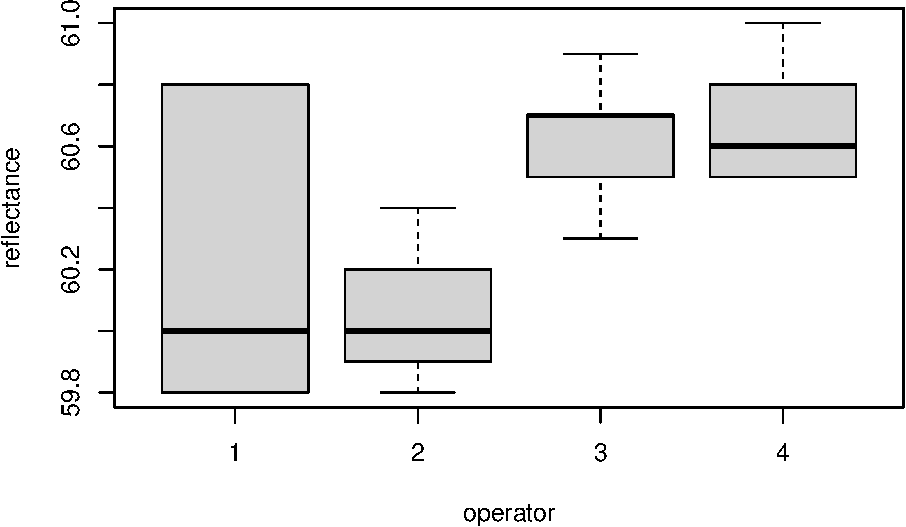
\includegraphics{bookdown_math3014-6027_files/figure-latex/pulp-boxplot-1} 

}

\caption{Pulp experiment: distributions of reflectance from the four operators.}\label{fig:pulp-boxplot}
\end{figure}

Figure \ref{fig:pulp-boxplot} shows that, relative to the variation, there may be a difference in the mean response between treatments 1 and 2, and 3 and 4. In this chapter, we will see how to make this comparison formally using linear models, and to assess how the choice of design impacts our results.

\end{example}

Throughout this chapter we will assume the \(i\)th treatment is applied to \(n_i\) experimental unit, with total number of runs \(n = \sum_{i=1}^t n_i\) in the experiment.

\hypertarget{a-unit-treatment-linear-model}{%
\section{A unit-treatment linear model}\label{a-unit-treatment-linear-model}}

An appropriate, and common, model to describe data from such experiments when the response is continuous is given by

\begin{equation}
y_{ij} = \mu + \tau_i + \varepsilon_{ij}\,, \quad i = 1, \ldots, t; j = 1, \ldots, n_i\,, 
\label{eq:utm}
\end{equation}

where \(y_{ij}\) is the response from the \(j\)th application of treatment \(i\), \(\mu\) is a constant parameter, \(\tau_i\) is the effect of the \(i\)th treatment, and \(\varepsilon_{ij}\) is the random individual effect from each experimental unit with \(E(\varepsilon_{ij})=0\) and \(\mathrm{Var}(\varepsilon_{ij}) = \sigma^2\). All random errors are assumed independent and here we also assume \(\varepsilon_{ij} \sim N(0, \sigma^2)\).

Model \eqref{eq:utm} assumes that each treatment can be randomly allocated to one of the \(n\) experimental units, and that the response observed is independent of the allocation of all the other treatments (the stable unit treatment value assumption or SUTVA).

Why is this model appropriate and commonly used? The expected response from the application of the \(i\)th treatment is

\[
E(y_{ij}) = \mu + \tau_i\,.
\]
The parameter \(\mu\) can be thought of as representing the impact of many different features particular to \textbf{this} experiment but common to all units, and \(\tau_i\) is the deviation due to applying treatment \(i\). From the applicable of two different hypothetical experiments, A and B, the expected response from treatment \(i\) may be different due to a different overall mean. From experiment A:

\[
E(y_{ij}) = \mu_{\mathrm{A}} + \tau_i\,.
\]
From experiment B:
\[
E(y_{ij}) = \mu_{\mathrm{B}} + \tau_i\,.
\]
But the \textbf{difference} between treatments \(k\) and \(l\) (\(k, l = 1,\ldots, t\))

\begin{align*}
E(y_{kj}) - E(y_{lj}) & = \mu_A + \tau_k - \mu_A - \tau_l \\
& = \tau_k - \tau_l\,,
\end{align*}

is constant across different experiments. This concept of \textbf{comparison} underpins most design of experiments, and will be applied throughout this module.

\hypertarget{the-partitioned-linear-model}{%
\section{The partitioned linear model}\label{the-partitioned-linear-model}}

In matrix form, we can write model \eqref{eq:utm} as

\[
\boldsymbol{y}= X_1\mu + X_2\boldsymbol{\tau}+ \boldsymbol{\varepsilon}\,,
\]
where \(X_1 = \boldsymbol{1}_n\), the \(n\)-vector with every entry equal to one,

\[
X_2 = \bigoplus_{i = 1}^t \boldsymbol{1}_{n_i} = \begin{bmatrix}
\boldsymbol{1}_{n_1} & \boldsymbol{0}_{n_1} & \cdots &  \boldsymbol{0}_{n_1} \\
\boldsymbol{0}_{n_2} & \boldsymbol{1}_{n_2} & \cdots &  \boldsymbol{0}_{n_2} \\
\vdots & & \ddots & \vdots \\
\boldsymbol{0}_{n_t} & \boldsymbol{0}_{n_t} & \cdots &  \boldsymbol{1}_{n_t} \\
\end{bmatrix}\,,
\]
with \(\bigoplus\) denoting ``direct sum'', \(\boldsymbol{0}_{n_i}\) is the \(n_i\)-vector with every entry equal to zero, \(\boldsymbol{\tau}= [\tau_1, \ldots, \tau_t]^{\mathrm{T}}\) and \(\boldsymbol{\varepsilon}= [\varepsilon_{11}, \ldots, \varepsilon_{tn_t}]^{\mathrm{T}}\).

Why are we partitioning the model? Going back to our discussion of the role of \(\mu\) and \(\tau_i\), it is clear that we not interested in estimating \(\mu\), which represents an experiment-specific contribution to the expected mean. Our only interest is in estimating the (differences between the) \(\tau_i\). Hence, we can treat \(\mu\) as a nuisance parameter.

If we define \(X = [X_1\, \vert\, X_2]\) and \(\boldsymbol{\beta}^{\mathrm{T}} = [\mu \vert \boldsymbol{\tau}^{\mathrm{T}}]\), we can write the usual least squares equations

\begin{equation}
X^{\mathrm{T}}X\hat{\boldsymbol{\beta}} = X^{\mathrm{T}}\boldsymbol{y}
\label{eq:crd-ls}
\end{equation}
as a system of two matrix equations

\begin{align*}
X_1^{\mathrm{T}}X_1\hat{\mu} + X_1^{\mathrm{T}}X_2\hat{\boldsymbol{\tau}} & = X_1^{\mathrm{T}}\boldsymbol{y}\\
X_2^{\mathrm{T}}X_1\hat{\mu} + X_2^{\mathrm{T}}X_2\hat{\boldsymbol{\tau}} & = X_2^{\mathrm{T}}\boldsymbol{y}\,. \\
\end{align*}

Assuming \((X_1^{\mathrm{T}}X_1)^{-1}\) exists, which it does in this case, we can pre-multiply the first of these equations by \(X_2^{\mathrm{T}}X_1(X_1^{\mathrm{T}}X_1)^{-1}\) and subtract it from the second equation to obtain

\begin{align*}
X_2^{\mathrm{T}}[I_n - X_1(X_1^{\mathrm{T}}X_1)^{-1}X_1^{\mathrm{T}}]X_1\hat{\mu} 
& + X_2^{\mathrm{T}}[I_n - X_1(X_1^{\mathrm{T}}X_1)^{-1}X_1^{\mathrm{T}}]X_2\hat{\boldsymbol{\tau}} \\
& = X_2^{\mathrm{T}}[I_n - X_1(X_1^{\mathrm{T}}X_1)^{-1}X_1^{\mathrm{T}}]\boldsymbol{y}\,.
\end{align*}

Writing \(H_1 = X_1(X_1^{\mathrm{T}}X_1)^{-1}X_1^{\mathrm{T}}\), we obtain

\begin{equation}
X_2^{\mathrm{T}}[I_n - H_1]X_1\hat{\mu} + X_2^{\mathrm{T}}[I_n - H_1]X_2\hat{\boldsymbol{\tau}} = X_2^{\mathrm{T}}[I_n - H_1]\boldsymbol{y}\,.
\label{eq:almost-reduced}
\end{equation}
The matrix \(H_1\) is a ``hat'' matrix for a linear model containing only the term \(\mu\), and hence \(H_1X_1 = X_1\) (see MATH2010 or STAT6123). Hence the first term in \eqref{eq:almost-reduced} is zero, and we obtain the \textbf{reduced normal equations} for \(\boldsymbol{\tau}\):

\begin{equation}
X_2^{\mathrm{T}}[I_n - H_1]X_2\hat{\boldsymbol{\tau}} = X_2^{\mathrm{T}}[I_n - H_1]\boldsymbol{y}\,.
\label{eq:crd-red-normal}
\end{equation}

Note that the solutions from \eqref{eq:crd-red-normal} are not different from the solution to \(\hat{\boldsymbol{\tau}}\) that would be obtained from solving \eqref{eq:crd-ls}; equation \eqref{eq:crd-red-normal} is simply a re-expression, where we have eliminated the nuisance parameter \(\mu\). This fact means that we rarely need to solve \eqref{eq:crd-red-normal} explicitly.

Recalling that for a hat matrix, \(I_n - H_1\) is idempotent and symmetric (see MATH2010 or MATH6174), if we define

\[
X_{2|1} = (I_n - H_1)X_2\,,
\]
then we can rewrite equation \eqref{eq:crd-red-normal} as

\begin{equation}
X_{2|1}^{\mathrm{T}}X_{2|1}\hat{\boldsymbol{\tau}} = X_{2|1}^{\mathrm{T}}\boldsymbol{y}\,, 
\label{eq:rne}
\end{equation}

which are the normal equations for a linear model with expectation \(E(\boldsymbol{y}) = X_{2|1}\boldsymbol{\tau}\).

\hypertarget{reduced-normal-equations-for-the-crd}{%
\section{Reduced normal equations for the CRD}\label{reduced-normal-equations-for-the-crd}}

For the CRD discussed in this chapter, \(X_1^{\mathrm{T}}X_1 = n\), the total number of runs in the experiment\footnote{In later chapters we will see examples where \(X_1\) has \(>1\) columns, and hence \(X_1^{\mathrm{T}}X_1\) is a matrix.}. Hence \((X_1^{\mathrm{T}}X_1)^{-1} = 1/n\) and \(H_1 = \frac{1}{n}J_n\), with \(J_n\) the \(n\times n\) matrix with all entries equal to 1.

The adjusted model matrix then has the form

\begin{align}
X_{2|1} & = (I_n - H_1)X_2 \nonumber\\
& = X_2 - \frac{1}{n}J_nX_2 \nonumber\\
& = X_2 - \frac{1}{n}[n_1\boldsymbol{1}_n \vert \cdots \vert n_t\boldsymbol{1}_n]\,. \label{eq:crd-x21} 
\end{align}

That is, every column of \(X_2\) has been adjusted by the subtraction of the column mean from each entry\footnote{Often called ``column centred''}. Also notice that each row of \(X_{2|1}\) has a row-sum equal to zero (\(= 1 - \sum_{i=1}^tn_t/n\)). Hence, \(X_{2|1}\) is not of full column rank, and so the reduced normal equations do not have a unique solution\footnote{If we recalled the material on ``dummy'' variables from MATH2010 or STAT6123, we would already have realised this.}.

Although \eqref{eq:rne}, and hence, \eqref{eq:crd-ls}, have no unique solution\footnote{That is, for any two solutions \(\tilde{\boldsymbol{\beta}}_1\) and \(\tilde{\boldsymbol{\beta}}_2\), \(X\tilde{\boldsymbol{\beta}}_1 = \tilde{\boldsymbol{\beta}}_1\).}, it can be shown that both \(\widehat{X_{2|1}\boldsymbol{\tau}}\) and \(\widehat{X\boldsymbol{\beta}}\) have unique solutions. Hence fitted values \(\hat{\boldsymbol{y}} = \widehat{X\boldsymbol{\beta}}\) and the residual sum of squares

\[
RSS = \left(\boldsymbol{y}- \widehat{X\boldsymbol{\beta}}\right)^{\mathrm{T}}\left(\boldsymbol{y}- \widehat{X\boldsymbol{\beta}}\right)
\]
are both uniquely defined for any solution to \eqref{eq:crd-ls}. That is, every solution to the normal equations leads to the same fitted values and residual sum of squares.

In MATH2010 and STAT6123 we fitted models with categorical variables by defining a set of dummy variables and estimating a reduced model. Here, we will take a slightly different approach and study which combinations of parameters from \eqref{eq:utm} are estimable, and in particular which linear combinations of the treatment parameters \(\tau_i\) we can estimate.

Let's study equation \eqref{eq:rne} in more detail. We have

\begin{align*}
X^{\mathrm{T}}_{2|1}X_{2|1} & = X_2^{\mathrm{T}}(I_n - H_1)X_2 \\
 & = X_2^{\mathrm{T}}X_2 - X_2^{\mathrm{T}}H_1X_2 \\
 & = \mathrm{diag}(\boldsymbol{n}) - \frac{1}{n}X_2^{\mathrm{T}}J_nX_2 \\
 & = \mathrm{diag}(\boldsymbol{n}) - \frac{1}{n}\boldsymbol{n}\boldsymbol{n}^{\mathrm{T}}\,,
\end{align*}

where \(\boldsymbol{n}^{\mathrm{T}} = (n_1, \ldots, n_t)\). Hence, the reduced normal equations become

\begin{align}
\left[\mathrm{diag}(\boldsymbol{n}) - \frac{1}{n}\boldsymbol{n}\boldsymbol{n}^{\mathrm{T}}\right]\hat{\boldsymbol{\tau}} & = X_2^{\mathrm{T}}\boldsymbol{y}- \frac{1}{n}X_2^{\mathrm{T}}J_n\boldsymbol{y}\\
& = X_2^{\mathrm{T}}\boldsymbol{y}- \boldsymbol{n}\bar{y}_{..}\,,
\label{eq:crd-rne}
\end{align}

where \(\bar{y}_{..} = \frac{1}{n}\sum_{i = 1}^t\sum_{j = 1}^{n_i} y_{ij}\), i.e.~the overall average of the observations from the experiment.

From \eqref{eq:crd-rne} we obtain a system of \(t\) equations, each having the form

\begin{equation}
\hat{\tau}_i - \hat{\tau}_w = \bar{y}_{i.} - \bar{y}_{..}\,,
\label{eq:crd-irne}
\end{equation}

where \(\hat{\tau}_w = \frac{1}{n}\sum_{i=1}^tn_i\hat{\tau}_i\) and \(\bar{y}_{i.} = \frac{1}{n_i}\sum_{j = 1}^{n_i}y_{ij}\) \((i = 1, \ldots, t)\).

These \(t\) equations are not independent; when multiplied by the \(n_i\), they sum to zero due to the linear dependency between the columns of \(X_{2|1}\). Hence, there is no unique solution to \(\hat{\boldsymbol{\tau}}\) from equation \eqref{eq:crd-rne}. However, we can estimate certain linear combinations of the \(\tau_i\), called \emph{contrasts}.

\hypertarget{contrasts}{%
\section{Contrasts}\label{contrasts}}

\begin{definition}
\protect\hypertarget{def:contrast}{}\label{def:contrast}

A treatment \textbf{contrast} is a linear combination \(\boldsymbol{c}^{\mathrm{T}}\boldsymbol{\tau}\) with coefficient vector \(\boldsymbol{c}^{\mathrm{T}} = (c_1,\ldots, c_t)\) such that \(\boldsymbol{c}^{\mathrm{T}}\boldsymbol{1} = 0\); that is, \(\sum_{i = 1}^t c_i = 0\).

\end{definition}

For example, assume we have \(t = 3\) treatments, then the following vectors \(\boldsymbol{c}\) all define contrasts:

\begin{enumerate}
\def\labelenumi{\arabic{enumi}.}
\tightlist
\item
  \(\boldsymbol{c}^{\mathrm{T}} = (1, -1, 0)\),
\item
  \(\boldsymbol{c}^{\mathrm{T}} = (1, 0, -1)\),
\item
  \(\boldsymbol{c}^{\mathrm{T}} = (0, 1, -1)\).
\end{enumerate}

In fact, they define all \({3\choose 2} = 3\) pairwise comparisons between treatments. The following are also contrasts:

\begin{enumerate}
\def\labelenumi{\arabic{enumi}.}
\setcounter{enumi}{3}
\tightlist
\item
  \(\boldsymbol{c}^{\mathrm{T}} = (2, -1, -1)\),
\item
  \(\boldsymbol{c}^{\mathrm{T}} = (0.5, -1, 0.5)\),
\end{enumerate}

each comparing the sum, or average, of expected responses from two treatments to the expected response from the remaining treatment.

The following are not contrasts, as \(\boldsymbol{c}^{\mathrm{T}}\boldsymbol{1} \ne 0\):

\begin{enumerate}
\def\labelenumi{\arabic{enumi}.}
\setcounter{enumi}{5}
\tightlist
\item
  \(\boldsymbol{c}^{\mathrm{T}} = (2, -1, 0)\),
\item
  \(\boldsymbol{c}^{\mathrm{T}} = (1, 0, 0)\),
\end{enumerate}

with the final example once again demonstrating that we cannot estimate the individual \(\tau_i\).

\hypertarget{contrast-crd}{%
\section{Treatment contrast estimators in the CRD}\label{contrast-crd}}

We estimate a treatment contrast \(\boldsymbol{c}^{\mathrm{T}}\boldsymbol{\tau}\) in the CRD via linear combinations of equations \eqref{eq:crd-irne}:

\begin{align*}
& \sum_{i=1}^t c_i\hat{\tau}_i - \sum_{i=1}^tc_i\hat{\tau}_w = \sum_{i=1}^tc_i\bar{y}_{i.} - \sum_{i=1}^tc_i\bar{y}_{..} \\
\Rightarrow & \sum_{i=1}^t c_i\hat{\tau}_i = \sum_{i=1}^tc_i\bar{y}_{i.}\,,
\end{align*}

as \(\sum_{i=1}^tc_i\hat{\tau}_w = \sum_{i=1}^tc_i\bar{y}_{..} = 0\), as \(\sum_{i=1}^tc_i = 0\). Hence, the unique estimator of the contrast \(\boldsymbol{c}^{\mathrm{T}}\boldsymbol{\tau}\) has the form

\[
\widehat{\boldsymbol{c}^{\mathrm{T}}\boldsymbol{\tau}} = \sum_{i=1}^tc_i\bar{y}_{i.}\,.
\]
That is, we estimate the contrast in the treatment effects by the corresponding contrast in the treatment means.

The variance of this estimator is straightforward to obtain:

\begin{align*}
\mathrm{var}\left(\widehat{\boldsymbol{c}^{\mathrm{T}}\boldsymbol{\tau}}\right) 
& = \sum_{i=1}^tc_i^2\mathrm{var}(\bar{y}_{i.}) \\
& = \sigma^2\sum_{i=1}^tc_i^2/n_i\,,
\end{align*}

as, under our model assumptions, each \(\bar{y}_{i.}\) is an average of independent observations with variance \(\sigma^2\). Similarly, from model \eqref{eq:utm} we can derive the distribution of \(\widehat{\boldsymbol{c}^{\mathrm{T}}\boldsymbol{\tau}}\) as

\[
\widehat{\boldsymbol{c}^{\mathrm{T}}\boldsymbol{\tau}} \sim N\left(\boldsymbol{c}^{\mathrm{T}}\boldsymbol{\tau}, \sigma^2\sum_{i=1}^tc_i^2/n_i\right)\,.
\]
Confidence intervals and hypothesis tests for \(\boldsymbol{c}^{\mathrm{T}}\boldsymbol{\tau}\) can be constructed/conducted using this distribution, e.g.

\begin{itemize}
\tightlist
\item
  a \(100(1-\frac{\alpha}{2})\)\% confidence interval:
  \[
   \boldsymbol{c}^{\mathrm{T}}\boldsymbol{\tau} \in \sum_{i=1}^tc_i\bar{y}_{i.} \pm t_{n-t, 1-\frac{\alpha}{2}}s\sqrt{\sum_{i=1}^tc_i^2/n_i}\,,
   \]
\end{itemize}

where \(t_{n-t, 1-\frac{\alpha}{2}}\) is the \(1-\frac{\alpha}{2}\) quantile of a \(t\)-distribution with \(n-t\) degrees of freedom and

\begin{equation} 
s^2 = \frac{1}{n-t}\sum_{i=1}^t\sum_{j=1}^{n_i}(y_{ij} - \bar{y}_{i.})^2
\label{eq:crd-s2}
\end{equation}

is the estimate of \(\sigma^2\).

\begin{itemize}
\tightlist
\item
  the hypothesis \(H_0: \boldsymbol{c}^{\mathrm{T}}\boldsymbol{\tau} = 0\) against the two-sided alternative \(H_1: \boldsymbol{c}^{\mathrm{T}}\boldsymbol{\tau} \ne 0\) is rejected using a test of with confidence level \(1-\alpha/2\) if
\end{itemize}

\[
 \frac{|\sum_{i=1}^tc_i\bar{y}_{i.}|}{s\sqrt{\sum_{i=1}^tc_i^2/n_i}} > t_{n-t, 1-\frac{\alpha}{2}}\,.
 \]

\hypertarget{r-crd}{%
\section{Analysing CRDs in R}\label{r-crd}}

Let's return to Example \ref{exm:one-way}.

\begin{Shaded}
\begin{Highlighting}[]
\NormalTok{knitr}\SpecialCharTok{::}\FunctionTok{kable}\NormalTok{(}
\NormalTok{ tidyr}\SpecialCharTok{::}\FunctionTok{pivot\_wider}\NormalTok{(pulp, }\AttributeTok{names\_from =}\NormalTok{ operator, }\AttributeTok{values\_from =}\NormalTok{ reflectance)[, }\SpecialCharTok{{-}}\DecValTok{1}\NormalTok{],}
 \AttributeTok{col.names =} \FunctionTok{paste}\NormalTok{(}\StringTok{"Operator"}\NormalTok{, }\DecValTok{1}\SpecialCharTok{:}\DecValTok{4}\NormalTok{),}
 \AttributeTok{caption =} \StringTok{"Pulp experiment: reflectance values (unitless) from four different operators."}
\NormalTok{)}
\end{Highlighting}
\end{Shaded}

\begin{table}

\caption{\label{tab:one-way-analysis}Pulp experiment: reflectance values (unitless) from four different operators.}
\centering
\begin{tabular}[t]{r|r|r|r}
\hline
Operator 1 & Operator 2 & Operator 3 & Operator 4\\
\hline
59.8 & 59.8 & 60.7 & 61.0\\
\hline
60.0 & 60.2 & 60.7 & 60.8\\
\hline
60.8 & 60.4 & 60.5 & 60.6\\
\hline
60.8 & 59.9 & 60.9 & 60.5\\
\hline
59.8 & 60.0 & 60.3 & 60.5\\
\hline
\end{tabular}
\end{table}

Clearly, we could directly calculate, and then compare, mean responses for each operator. However, there are (at least) two other ways we can proceed which use the fact we are fitting a linear model. These will be useful when we consider more complex models.

\begin{enumerate}
\def\labelenumi{\arabic{enumi}.}
\item
  Using \texttt{pairwise.t.test}.

\begin{Shaded}
\begin{Highlighting}[]
\FunctionTok{with}\NormalTok{(pulp, }
 \FunctionTok{pairwise.t.test}\NormalTok{(reflectance, operator, }\AttributeTok{p.adjust.method =} \StringTok{\textquotesingle{}none\textquotesingle{}}\NormalTok{))}
\end{Highlighting}
\end{Shaded}

\begin{verbatim}
## 
##  Pairwise comparisons using t tests with pooled SD 
## 
## data:  reflectance and operator 
## 
##   1     2     3    
## 2 0.396 -     -    
## 3 0.084 0.015 -    
## 4 0.049 0.008 0.775
## 
## P value adjustment method: none
\end{verbatim}

  This function performs hypothesis tests for all pairwise treatment comparisons (with a default confidence level of 0.95). Here we can see that operators 1 and 4, 2 and 3, and 2 and 4 have statistically significant differences.
\item
  Using \texttt{lm} and the \texttt{emmeans} package.

\begin{Shaded}
\begin{Highlighting}[]
\NormalTok{pulp.lm }\OtherTok{\textless{}{-}} \FunctionTok{lm}\NormalTok{(reflectance }\SpecialCharTok{\textasciitilde{}}\NormalTok{ operator, }\AttributeTok{data =}\NormalTok{ pulp)}
\FunctionTok{anova}\NormalTok{(pulp.lm)}
\end{Highlighting}
\end{Shaded}

\begin{verbatim}
## Analysis of Variance Table
## 
## Response: reflectance
##           Df Sum Sq Mean Sq F value Pr(>F)  
## operator   3   1.34   0.447     4.2  0.023 *
## Residuals 16   1.70   0.106                 
## ---
## Signif. codes:  0 '***' 0.001 '**' 0.01 '*' 0.05 '.' 0.1 ' ' 1
\end{verbatim}

\begin{Shaded}
\begin{Highlighting}[]
\NormalTok{pulp.emm }\OtherTok{\textless{}{-}}\NormalTok{ emmeans}\SpecialCharTok{::}\FunctionTok{emmeans}\NormalTok{(pulp.lm, }\SpecialCharTok{\textasciitilde{}}\NormalTok{ operator)}
\FunctionTok{pairs}\NormalTok{(pulp.emm, }\AttributeTok{adjust =} \StringTok{\textquotesingle{}none\textquotesingle{}}\NormalTok{)}
\end{Highlighting}
\end{Shaded}

\begin{verbatim}
##  contrast estimate    SE df t.ratio p.value
##  1 - 2        0.18 0.206 16   0.873  0.3955
##  1 - 3       -0.38 0.206 16  -1.843  0.0839
##  1 - 4       -0.44 0.206 16  -2.134  0.0486
##  2 - 3       -0.56 0.206 16  -2.716  0.0153
##  2 - 4       -0.62 0.206 16  -3.007  0.0083
##  3 - 4       -0.06 0.206 16  -0.291  0.7748
\end{verbatim}

  Here, we have first fitted the linear model object. The \texttt{lm} function, by default, will have set up dummy variables with the first treatment (operator) as a baseline (see MATH2010 or STAT6123). We then take the intermediate step of calculating the ANOVA table for this experiment, and use an F-test to compare the model accounting for operator differences to the null model; there are differences between operators at the 5\% significance level,

  The choice of dummy variables in the linear model is unimportant; any set could be used\footnote{Recall that although \(\mu\) and \(\boldsymbol{\tau}\) are not uniquely estimable, fitted values \(\hat{y}_i = \hat{\mu} + \hat{\tau}_i\) \textbf{are}, and hence it does not matter which dummy variables we use in \texttt{lm}.}, as in the next line we use the \texttt{emmeans} function (from the package of the same name) to specify that we are interested in estimating contrasts in the factor \texttt{operator} (which specifies our treatments in this experiment). Finally, the \texttt{pairs} command performs hypothesis tests for all pairwise comparisons between the four treatments. The results are the same as those obtained from using \texttt{pairwise.t.test}.
\end{enumerate}

Our preferred approach is using method 2 (\texttt{lm} and \texttt{emmeans}), for four main reasons:

\begin{enumerate}
\def\labelenumi{\alph{enumi}.}
\item
  The function \texttt{contrasts} in the \texttt{emmeans} package can be used to estimate arbitrary treatment contrasts (see \texttt{help("contrast-methods")}).

\begin{Shaded}
\begin{Highlighting}[]
\CommentTok{\# same as \textasciigrave{}pairs\textasciigrave{} above}
\NormalTok{emmeans}\SpecialCharTok{::}\FunctionTok{contrast}\NormalTok{(pulp.emm, }\StringTok{"pairwise"}\NormalTok{, }\AttributeTok{adjust =} \StringTok{"none"}\NormalTok{)}
\end{Highlighting}
\end{Shaded}

\begin{verbatim}
##  contrast estimate    SE df t.ratio p.value
##  1 - 2        0.18 0.206 16   0.873  0.3955
##  1 - 3       -0.38 0.206 16  -1.843  0.0839
##  1 - 4       -0.44 0.206 16  -2.134  0.0486
##  2 - 3       -0.56 0.206 16  -2.716  0.0153
##  2 - 4       -0.62 0.206 16  -3.007  0.0083
##  3 - 4       -0.06 0.206 16  -0.291  0.7748
\end{verbatim}

\begin{Shaded}
\begin{Highlighting}[]
\CommentTok{\# estimating single contrast c = (1, {-}.5, {-}.5)}
\CommentTok{\# comparing operator 1 with operators 2 and 3}
\NormalTok{contrast1v23.emmc }\OtherTok{\textless{}{-}} \ControlFlowTok{function}\NormalTok{(levs) }
  \FunctionTok{data.frame}\NormalTok{(}\StringTok{\textquotesingle{}t1 v avg t2 t3\textquotesingle{}} \OtherTok{=} \FunctionTok{c}\NormalTok{(}\DecValTok{1}\NormalTok{, }\SpecialCharTok{{-}}\NormalTok{.}\DecValTok{5}\NormalTok{, }\SpecialCharTok{{-}}\NormalTok{.}\DecValTok{5}\NormalTok{, }\DecValTok{0}\NormalTok{))}
\NormalTok{emmeans}\SpecialCharTok{::}\FunctionTok{contrast}\NormalTok{(pulp.emm, }\StringTok{\textquotesingle{}contrast1v23\textquotesingle{}}\NormalTok{)}
\end{Highlighting}
\end{Shaded}

\begin{verbatim}
##  contrast       estimate    SE df t.ratio p.value
##  t1.v.avg.t2.t3     -0.1 0.179 16  -0.560  0.5832
\end{verbatim}
\item
  It more easily generalises to the more complicated models we will see in Chapter \ref{blocking}.
\item
  It explicitly acknowledges that we have fitted a linear model, and so encourages us to check the model assumptions (see \protect\hyperlink{nap-black-ex}{Exercise 3}).
\item
  It is straightfoward to apply adjustments for \protect\hyperlink{multiple-comp}{multiple comparisons}.
\end{enumerate}

\hypertarget{multiple-comp}{%
\section{Multiple comparisons}\label{multiple-comp}}

When we perform hypothesis testing, we choose the critical region (i.e.~the rule that decides if we reject \(H_0\)) to control the probability of a type I error; that is, we control the probability of incorrectly rejecting \(H_0\). If we need to test multiple hypotheses, e.g.~to test all pairwise differences, we need to consider the overall probability of incorrectly rejecting \textbf{one or more} null hypothesis. This is called the \textbf{experiment-wise} or \textbf{family-wise} error rate.

For Example \ref{exm:one-way}, there are \({4 \choose 2} = 6\) pairwise comparisons. Under the assumption that all tests are independent\footnote{They aren't, but it simplifies the maths!}, assuming each individual test has type I error 0.05, the experiment-wise type I error rate is given by:

\begin{Shaded}
\begin{Highlighting}[]
\NormalTok{alpha }\OtherTok{\textless{}{-}} \FloatTok{0.05}
\DecValTok{1} \SpecialCharTok{{-}}\NormalTok{ (}\DecValTok{1} \SpecialCharTok{{-}}\NormalTok{ alpha)}\SpecialCharTok{\^{}}\DecValTok{6}
\end{Highlighting}
\end{Shaded}

\begin{verbatim}
## [1] 0.2649
\end{verbatim}

An experiment-wise error rate of 0.2649 is substantially greater than 0.05. Hence, we would expect to make many more type I errors than may be desirable. \href{https://xkcd.com/882}{xkcd} has a fun example:

\begin{Shaded}
\begin{Highlighting}[]
\NormalTok{alpha }\OtherTok{\textless{}{-}} \FloatTok{0.05}
\DecValTok{1} \SpecialCharTok{{-}}\NormalTok{ (}\DecValTok{1} \SpecialCharTok{{-}}\NormalTok{ alpha)}\SpecialCharTok{\^{}}\DecValTok{20}
\end{Highlighting}
\end{Shaded}

\begin{verbatim}
## [1] 0.6415
\end{verbatim}

Therefore it is usually desirable to maintain some control of the experiment-wise type I error rate. We will consider two methods.

\begin{enumerate}
\def\labelenumi{\arabic{enumi}.}
\item
  The \textbf{Bonferroni method}. An upper bound on the experiment-wise type I error rate for testing \(k\) hypotheses can be shown to be

  \begin{align*}
  P(\mbox{wrongly reject at least one of } H_{0}^1, \ldots, H_{0}^k) = &    P\left(\bigcup_{i=1}^{k}\{\mbox{wrongly reject } H_{0}^i\}\right) \\
  & \leq \sum_{i=1}^{k}\underbrace{P(\mbox{wrongly reject } H_{0}^i)}_{\leq \alpha} \\ 
  & \leq k\alpha\,.
  \end{align*}

  Hence a \emph{conservative}\footnote{So the experiment-wise type I error will actually be less than the prescribed \(\alpha\)} adjustment for multiple comparisons is to test each hypothesis at size \(\alpha / k\), i.e.~for the CRD compare to the quantile \(t_{n-t, 1-\frac{\alpha}{2k}}\) (or multiply each individual p-value by \(k\)).

  For Example \ref{exm:one-way}, we can test all pairwise comparisons, each at size \(\alpha/k\) using the \texttt{adjustment} argument in \texttt{pairs}.

\begin{Shaded}
\begin{Highlighting}[]
\FunctionTok{pairs}\NormalTok{(pulp.emm, }\AttributeTok{adjust =} \StringTok{\textquotesingle{}bonferroni\textquotesingle{}}\NormalTok{)}
\end{Highlighting}
\end{Shaded}

\begin{verbatim}
##  contrast estimate    SE df t.ratio p.value
##  1 - 2        0.18 0.206 16   0.873  1.0000
##  1 - 3       -0.38 0.206 16  -1.843  0.5034
##  1 - 4       -0.44 0.206 16  -2.134  0.2918
##  2 - 3       -0.56 0.206 16  -2.716  0.0915
##  2 - 4       -0.62 0.206 16  -3.007  0.0501
##  3 - 4       -0.06 0.206 16  -0.291  1.0000
## 
## P value adjustment: bonferroni method for 6 tests
\end{verbatim}

  Now, only one comparison is significant at an experiment-wise type I error rate of \(\alpha = 0.05\) (operators 2 and 4).
\item
  \textbf{Tukey's method}. An alternative approach that gives an exact experiment-wise error rate of \(100\alpha\)\% compares the \(t\) statistic to a critical value from the studentised range distribution\footnote{Given two independent samples \(u_1, \ldots, u_l\) and \(v_1,\ldots,v_m\) from the same distribution, the studentised range distribution is the distribution of \(\frac{R}{\sqrt{2}S}\), where \(R = u_{max}-u_{min}\) is the range of the first sample, and \(S = \sqrt{\frac{1}{m-1}\sum_{i=1}^m(v_i - \bar{v})^2}\) be the sample standard deviation of the second sample.}, given by \(\frac{1}{\sqrt{2}}q_{t, n-t, 1-\alpha}\) with \(q_{t, n-t, 1-\alpha}\) the \(1-\alpha\) quantile from the studentised range distribution (available in \texttt{R} as \texttt{qtukey}).

  For Example \ref{exm:one-way}:

\begin{Shaded}
\begin{Highlighting}[]
\FunctionTok{pairs}\NormalTok{(pulp.emm)}
\end{Highlighting}
\end{Shaded}

\begin{verbatim}
##  contrast estimate    SE df t.ratio p.value
##  1 - 2        0.18 0.206 16   0.873  0.8185
##  1 - 3       -0.38 0.206 16  -1.843  0.2903
##  1 - 4       -0.44 0.206 16  -2.134  0.1845
##  2 - 3       -0.56 0.206 16  -2.716  0.0658
##  2 - 4       -0.62 0.206 16  -3.007  0.0377
##  3 - 4       -0.06 0.206 16  -0.291  0.9911
## 
## P value adjustment: tukey method for comparing a family of 4 estimates
\end{verbatim}
\end{enumerate}

The default adjustment in the \texttt{pairs} function is the Tukey method. Comparing the p-values for each comparison using unadjusted t-tests, the Boneferroni and Tukey methods:

\begin{Shaded}
\begin{Highlighting}[]
\NormalTok{pairs.u }\OtherTok{\textless{}{-}} \FunctionTok{pairs}\NormalTok{(pulp.emm, }\AttributeTok{adjust =} \StringTok{\textquotesingle{}none\textquotesingle{}}\NormalTok{)}
\NormalTok{pairs.b }\OtherTok{\textless{}{-}} \FunctionTok{pairs}\NormalTok{(pulp.emm, }\AttributeTok{adjust =} \StringTok{\textquotesingle{}bonferroni\textquotesingle{}}\NormalTok{)}
\NormalTok{pairs.t }\OtherTok{\textless{}{-}} \FunctionTok{pairs}\NormalTok{(pulp.emm)}
\FunctionTok{data.frame}\NormalTok{(}\FunctionTok{transform}\NormalTok{(pairs.b)[, }\DecValTok{1}\SpecialCharTok{:}\DecValTok{5}\NormalTok{], }\AttributeTok{Bonf.p.value =} \FunctionTok{transform}\NormalTok{(pairs.b)[, }\DecValTok{6}\NormalTok{], }\AttributeTok{Tukey.p.value =} \FunctionTok{transform}\NormalTok{(pairs.t)[, }\DecValTok{6}\NormalTok{], }\AttributeTok{unadjust.p.value =} \FunctionTok{transform}\NormalTok{(pairs.u)[, }\DecValTok{6}\NormalTok{])}
\end{Highlighting}
\end{Shaded}

\begin{verbatim}
##   contrast estimate     SE df t.ratio Bonf.p.value Tukey.p.value
## 1    1 - 2     0.18 0.2062 16  0.8731      1.00000       0.81854
## 2    1 - 3    -0.38 0.2062 16 -1.8433      0.50336       0.29030
## 3    1 - 4    -0.44 0.2062 16 -2.1343      0.29182       0.18448
## 4    2 - 3    -0.56 0.2062 16 -2.7164      0.09150       0.06579
## 5    2 - 4    -0.62 0.2062 16 -3.0074      0.05009       0.03767
## 6    3 - 4    -0.06 0.2062 16 -0.2910      1.00000       0.99108
##   unadjust.p.value
## 1         0.395509
## 2         0.083893
## 3         0.048637
## 4         0.015251
## 5         0.008349
## 6         0.774758
\end{verbatim}

Although the decision on which hypotheses to reject (comparson 2 - 4) is the same here for both methods, the p-values from the Bonferroni method are all larger, reflecting its more conservative nature.

\hypertarget{impact-of-design-choices-on-estimation}{%
\section{Impact of design choices on estimation}\label{impact-of-design-choices-on-estimation}}

Recall from Section \ref{contrast-crd} that the width of a confidence interval for a contrast \(\boldsymbol{c}^{\mathrm{T}}\boldsymbol{\tau}\) is given by \(2t_{n-t, 1-\frac{\alpha}{2}}s\sqrt{\sum_{i=1}^tc_i^2/n_i}\). The expectation of the square of this quantity is given by

\[
4t^2_{n-t, 1-\frac{\alpha}{2}}\sigma^2\sum_{i=1}^tc_i^2/n_i\,,
\]
as \(E(s^2) = \sigma^2\). It is intuitive that a good design should have small values of the square root of this quantity (divided by \(2\sigma\)),

\[
t_{n-t, 1-\frac{\alpha}{2}}\sqrt{\sum_{i=1}^tc_i^2/n_i}\,,
\]
which can be achieved either by increasing \(n\), and hence reducing the size of the \(t\)-quantile, or for choice of the \(n_i\) for a fixed \(n\), i.e.~through choice of replication of each treatment.

\hypertarget{crd-opt-all}{%
\subsection{Optimal treatment allocation}\label{crd-opt-all}}

It is quite common that although the total number, \(n\), of runs in the experiment may be fixed, the number \(n_1, n_2, \ldots, n_t\) applied to the different treatments is under the experimenter's control. Choosing \(n_1, n_2\) subject to \(n_1+n_2 = n\) was the first \textbf{optimal design} problem we encountered in Chapter \ref{intro}.

Assume interest lies in estimating the set of \(p\) contrasts \(\boldsymbol{c}_1^{\mathrm{T}}\boldsymbol{\tau}, \ldots, \boldsymbol{c}_p^{\mathrm{T}}\boldsymbol{\tau}\), with \(\boldsymbol{c}_l^{\mathrm{T}} = (c_{l1}, \ldots, c_{lt})\). One useful measure of the overall quality of the estimators of these \(p\) contrasts is the average variance, given by

\[
\sigma^2\sum_{l=1}^p\sum_{i=1}^tc_{li}^2/n_i\,.
\]
So we will minimise this variance by allocating larger values of \(n_i\) to the treatments with correspondingly larger values of the contrast coefficients \(c_{li}\). Therefore an approach to optimal allocation is to choose \(\boldsymbol{n} = (n_1, \ldots, n_t)^{\mathrm{T}}\) so as to

\begin{equation}
\mbox{minimise} \quad \phi(\boldsymbol{n}) = \sum_{l=1}^p\sum_{i=1}^tc_{li}^2/n_i\,\qquad \mbox{subject to} \quad \sum_{i=1}^tn_i = n\,.
\label{eq:opt-all}
\end{equation}

This is a discrete optimisation problem (the \(n_i\) are integers). It is usually easier to solve the relaxed problem, where we allow continuous \(0\le n_i \le n\), and round the resulting solution to obtain integers. There is no guarantee that such a rounded allocation will actually be the optimal integer-valued solution, but it is usually fairly close.

To solve the continuous version of \eqref{eq:opt-all} we will use the method of Lagrange mutliplers, where we define the function

\[
h(\boldsymbol{n}, \lambda) = \phi(\boldsymbol{n}) + \lambda\left(\sum_{i=1}^tn_i - n\right)\,,
\]
introducing the new scalar variable \(\lambda\), and solve the set of \(t+1\) equations:

\begin{align*}
\frac{\partial h}{\partial n_1} & = 0 \\
\vdots & \\
\frac{\partial h}{\partial n_t} & = 0 \\
\frac{\partial h}{\partial \lambda} & = 0\,.
\end{align*}

In this case, we have

\begin{equation}
\frac{\partial h}{\partial n_i} = -\sum_{l=1}^pc_{li}^2/n_i^2 + \lambda = 0\,,\quad i=1,\ldots t,
\label{eq:lm-ni}
\end{equation}
and
\[
\frac{\partial h}{\partial \lambda} = \sum_{i=1}^t n_i - n = 0\,.
\]
This last equation ensures \(\sum_{i=1}^tn_i = n\). From the \(t\) equations described by \eqref{eq:lm-ni}, we get

\[
n_i \propto \sqrt{\sum_{l=1}^pc_{li}^2}
\]
We don't need to explicitly solve for \(\lambda\) to find the normalising constant for each \(n_i\). As we know \(\sum_{i=1}^tn_i = n\), we obtain,

\begin{equation}
n_i = \frac{\sqrt{\sum_{l=1}^pc_{li}^2}}{\sum_{i=1}^t\sqrt{\sum_{l=1}^pc_{li}^2}}n\,.
\label{eq:opt-ni}
\end{equation}

Let's return to Example \ref{exm:one-way} and calculate the optimal allocations under two different sets of contrasts. First, we define an \texttt{R} function for calculating \eqref{eq:opt-ni}.

\begin{Shaded}
\begin{Highlighting}[]
\NormalTok{opt\_ni }\OtherTok{\textless{}{-}} \ControlFlowTok{function}\NormalTok{(C, n) \{}
\NormalTok{  CtC }\OtherTok{\textless{}{-}} \FunctionTok{t}\NormalTok{(C) }\SpecialCharTok{\%*\%}\NormalTok{ C}
\NormalTok{  n }\SpecialCharTok{*} \FunctionTok{sqrt}\NormalTok{(}\FunctionTok{diag}\NormalTok{(CtC)) }\SpecialCharTok{/} \FunctionTok{sum}\NormalTok{(}\FunctionTok{sqrt}\NormalTok{(}\FunctionTok{diag}\NormalTok{(CtC)))}
\NormalTok{\} }
\end{Highlighting}
\end{Shaded}

Checking that the function \texttt{opt-ni} matches \eqref{eq:opt-ni} is left as an exercise.

Consider two sets of contrasts:

\begin{enumerate}
\def\labelenumi{\arabic{enumi}.}
\item
  All pairwise comparisons between the four treatments
  \begin{align*}
  c_1 & = (-1, 1, 0, 0) \\
  c_2 & = (-1, 0, 1, 0) \\
  c_3 & = (-1, 0, 0, 1) \\
  c_4 & = (0, -1, 1, 0) \\
  c_5 & = (0, -1, 0, 1) \\
  c_6 & = (0, 0, -1, 1)\,.
  \end{align*}

  Calculating \eqref{eq:opt-ni}, we obtain

\begin{Shaded}
\begin{Highlighting}[]
\NormalTok{C }\OtherTok{\textless{}{-}} \FunctionTok{matrix}\NormalTok{(}
  \FunctionTok{c}\NormalTok{(}
\SpecialCharTok{{-}}\DecValTok{1}\NormalTok{, }\DecValTok{1}\NormalTok{, }\DecValTok{0}\NormalTok{, }\DecValTok{0}\NormalTok{,}
\SpecialCharTok{{-}}\DecValTok{1}\NormalTok{, }\DecValTok{0}\NormalTok{, }\DecValTok{1}\NormalTok{, }\DecValTok{0}\NormalTok{,}
\SpecialCharTok{{-}}\DecValTok{1}\NormalTok{, }\DecValTok{0}\NormalTok{, }\DecValTok{0}\NormalTok{, }\DecValTok{1}\NormalTok{,}
\DecValTok{0}\NormalTok{, }\SpecialCharTok{{-}}\DecValTok{1}\NormalTok{, }\DecValTok{1}\NormalTok{, }\DecValTok{0}\NormalTok{,}
\DecValTok{0}\NormalTok{, }\SpecialCharTok{{-}}\DecValTok{1}\NormalTok{, }\DecValTok{0}\NormalTok{, }\DecValTok{1}\NormalTok{,}
\DecValTok{0}\NormalTok{, }\DecValTok{0}\NormalTok{, }\SpecialCharTok{{-}}\DecValTok{1}\NormalTok{, }\DecValTok{1}\NormalTok{),}
  \AttributeTok{nrow =} \DecValTok{6}\NormalTok{, }\AttributeTok{byrow =}\NormalTok{ T}
\NormalTok{)}
\FunctionTok{opt\_ni}\NormalTok{(C, }\DecValTok{20}\NormalTok{)}
\end{Highlighting}
\end{Shaded}

\begin{verbatim}
## [1] 5 5 5 5
\end{verbatim}

  Hence confirming that equal replication of the treatments is optimal for minimising the average variance of estimators of the pairwise treatment differences.
\item
  If operator 4 is new to the mill, it may be desired to test their output to the average output from the other three operators, using a contrast with coefficients \(c = (1/3, 1/3, 1/3, -1)\). The allocation to minimise the variance of the corresponding estimator is given by:

\begin{Shaded}
\begin{Highlighting}[]
\NormalTok{C }\OtherTok{\textless{}{-}} \FunctionTok{matrix}\NormalTok{(}
  \FunctionTok{c}\NormalTok{(}\DecValTok{1}\SpecialCharTok{/}\DecValTok{3}\NormalTok{, }\DecValTok{1}\SpecialCharTok{/}\DecValTok{3}\NormalTok{, }\DecValTok{1}\SpecialCharTok{/}\DecValTok{3}\NormalTok{, }\SpecialCharTok{{-}}\DecValTok{1}\NormalTok{),}
  \AttributeTok{nrow =} \DecValTok{1}
\NormalTok{)}
\FunctionTok{opt\_ni}\NormalTok{(C, }\DecValTok{20}\NormalTok{)}
\end{Highlighting}
\end{Shaded}

\begin{verbatim}
## [1]  3.333  3.333  3.333 10.000
\end{verbatim}

  So the optimal allocation splits 10 units between operators 1-3, and allocates 10 units to operator 4. There is no exact integer rounding possible, so we will use \(n_1 = 4\), \(n_2=n_3 = 3\), \(n_4 = 10\) and calculate the efficiency by comparing the variance of this allocation to that from the equally allocated design.

\begin{Shaded}
\begin{Highlighting}[]
\NormalTok{crd\_var }\OtherTok{\textless{}{-}} \ControlFlowTok{function}\NormalTok{(C, n) \{}
\NormalTok{  CtC }\OtherTok{\textless{}{-}} \FunctionTok{t}\NormalTok{(C) }\SpecialCharTok{\%*\%}\NormalTok{ C}
  \FunctionTok{sum}\NormalTok{(}\FunctionTok{diag}\NormalTok{(CtC) }\SpecialCharTok{/}\NormalTok{ n)}
\NormalTok{\} }
\NormalTok{n\_equal }\OtherTok{\textless{}{-}} \FunctionTok{rep}\NormalTok{(}\DecValTok{5}\NormalTok{, }\DecValTok{4}\NormalTok{)}
\NormalTok{n\_opt }\OtherTok{\textless{}{-}} \FunctionTok{c}\NormalTok{(}\DecValTok{4}\NormalTok{, }\DecValTok{3}\NormalTok{, }\DecValTok{3}\NormalTok{, }\DecValTok{10}\NormalTok{)}
\FunctionTok{crd\_var}\NormalTok{(C, n\_opt) }\SpecialCharTok{/} \FunctionTok{crd\_var}\NormalTok{(C, n\_equal)}
\end{Highlighting}
\end{Shaded}

\begin{verbatim}
## [1] 0.7569
\end{verbatim}

  So the efficiency of the equally allocated design for estimating this contrast is 75.69 \%.
\end{enumerate}

\hypertarget{crd-size}{%
\subsection{Overall size of the experiment}\label{crd-size}}

We can also consider the complementary question: suppose the proportion of runs that is to be allocated to each treatment has been fixed in advance, what size of experiment should be performed to meet the objectives? That is, given a fixed proportion, \(w_i\), of resource to be allocated to the \(i\)th treatment, so that \(n_i = nw_i\) units will be allocated to that treatment, what value of \(n\) should be chosen?

One way of thinking about this question is to consider the ratio

\begin{align*}
\frac{|\boldsymbol{c}^{\mathrm{T}}\boldsymbol{\tau}|}{\sqrt{\mbox{Var}(\widehat{\boldsymbol{c}^{\mathrm{T}}\boldsymbol{\tau}})}} & = \frac{|\boldsymbol{c}^{\mathrm{T}}\boldsymbol{\tau}|}{\sqrt{\frac{\sigma^2}{n} \sum_{i=1}^tc_i^2/w_i}} \\
& = \sqrt{n}\frac{|\boldsymbol{c}^{\mathrm{T}}\boldsymbol{\tau}| / \sigma}{\sqrt{\sum_{i=1}^tc_i^2/w_i}}\,,
\end{align*}

which is analogous to the test statistic for \(H_0: \boldsymbol{c}^{\mathrm{T}}\boldsymbol{\tau} = 0\). For a given value of the signal-to-noise ratio \(d = |\boldsymbol{c}^{\mathrm{T}}\boldsymbol{\tau}| / \sigma\), we can choose \(n\) to result in a specified value of \(T = |\boldsymbol{c}^{\mathrm{T}}\boldsymbol{\tau}| / \sqrt{\mbox{Var}(\widehat{\boldsymbol{c}^{\mathrm{T}}\boldsymbol{\tau}})}\):

\[
n = T^2\frac{\sum_{i=1}^t c_i^2/w_i}{d^2}\,.
\]
Returning to Example \ref{exm:one-way}, assume are testing a single pairwise comparison and that we require \(T = 3\), so that the null hypothesis would be comfortably rejected at the 5\% level (cf 1.96 for a standard z-test). For equal allocation of the units to each treatment (\(w_1 = \cdots = w_4 = 1/4\)) and a variety of different values of the signal-to-noise ratio \(d\), we obtained the following optimal experiment sizes:

\begin{Shaded}
\begin{Highlighting}[]
\NormalTok{opt\_n }\OtherTok{\textless{}{-}} \ControlFlowTok{function}\NormalTok{(cv, prop, snr, target) target }\SpecialCharTok{\^{}} \DecValTok{2} \SpecialCharTok{*} \FunctionTok{c}\NormalTok{(}\FunctionTok{t}\NormalTok{(cv) }\SpecialCharTok{\%*\%} \FunctionTok{diag}\NormalTok{( }\DecValTok{1} \SpecialCharTok{/}\NormalTok{ prop) }\SpecialCharTok{\%*\%}\NormalTok{ cv) }\SpecialCharTok{/}\NormalTok{ snr }\SpecialCharTok{\^{}} \DecValTok{2}
\NormalTok{cv }\OtherTok{\textless{}{-}} \FunctionTok{c}\NormalTok{(}\SpecialCharTok{{-}}\DecValTok{1}\NormalTok{, }\DecValTok{1}\NormalTok{, }\DecValTok{0}\NormalTok{, }\DecValTok{0}\NormalTok{)}
\NormalTok{w }\OtherTok{\textless{}{-}} \FunctionTok{rep}\NormalTok{(}\DecValTok{1}\SpecialCharTok{/}\DecValTok{4}\NormalTok{, }\DecValTok{4}\NormalTok{)}
\NormalTok{snr }\OtherTok{\textless{}{-}} \FunctionTok{c}\NormalTok{(}\FloatTok{0.5}\NormalTok{, }\DecValTok{1}\NormalTok{, }\FloatTok{1.5}\NormalTok{, }\DecValTok{2}\NormalTok{, }\FloatTok{2.5}\NormalTok{, }\DecValTok{3}\NormalTok{)}
\FunctionTok{cbind}\NormalTok{(}\StringTok{\textquotesingle{}Signal{-}to{-}noise\textquotesingle{}} \OtherTok{=}\NormalTok{ snr, }\StringTok{\textquotesingle{}n\textquotesingle{}} \OtherTok{=} \FunctionTok{opt\_n}\NormalTok{(cv, w, snr, }\DecValTok{3}\NormalTok{))}
\end{Highlighting}
\end{Shaded}

\begin{verbatim}
##      Signal-to-noise      n
## [1,]             0.5 288.00
## [2,]             1.0  72.00
## [3,]             1.5  32.00
## [4,]             2.0  18.00
## [5,]             2.5  11.52
## [6,]             3.0   8.00
\end{verbatim}

So, for example, to achieve \(T = 3\) with a signal-to-noise ratio of \(d=0.5\) requires \(n=288\) runs. As would be expected, the number of runs required to achieve this value of \(T\) decreases as the signal-to-noise ration increases. For \(d=3\), only a very small experiment with \(n=8\) runs is needed.

\hypertarget{exercises-1}{%
\section{Exercises}\label{exercises-1}}

\begin{enumerate}
\def\labelenumi{\arabic{enumi}.}
\item
  \begin{enumerate}
  \def\labelenumii{\alph{enumii}.}
  \item
    For Example \ref{exm:one-way}, calculate the mean response for each operator and show that the treatment differences and results from hypothesis tests using the results in Section \ref{contrast-crd} are the same as those found in Section \ref{r-crd} using \texttt{pairwise.t.test}, and \texttt{emmeans}.
  \item
    Also check the results in Section \ref{multiple-comp} by (i) adjusting individual p-values (for Bonferroni) and (ii) using the \texttt{qtukey} command.
  \end{enumerate}
\end{enumerate}

Solution

As a reminder, the data from the experiment is as follows.

\begin{tabular}{r|r|r|r}
\hline
Operator 1 & Operator 2 & Operator 3 & Operator 4\\
\hline
59.8 & 59.8 & 60.7 & 61.0\\
\hline
60.0 & 60.2 & 60.7 & 60.8\\
\hline
60.8 & 60.4 & 60.5 & 60.6\\
\hline
60.8 & 59.9 & 60.9 & 60.5\\
\hline
59.8 & 60.0 & 60.3 & 60.5\\
\hline
\end{tabular}

The mean response, and variance, from each treatment is given by

\begin{tabular}{l|r|r|r}
\hline
operator & n\_i & mean & variance\\
\hline
1 & 5 & 60.24 & 0.268\\
\hline
2 & 5 & 60.06 & 0.058\\
\hline
3 & 5 & 60.62 & 0.052\\
\hline
4 & 5 & 60.68 & 0.047\\
\hline
\end{tabular}

The sample variance, \(s^2 = 0.106\), from \eqref{eq:crd-s2}. As \(\sum_{i=1}^tc_i^2/n_i = \frac{2}{5}\) for contrast vectors \(\boldsymbol{c}\) corresponding to pairwise differences, the standard error of each pairwise difference is given by \(\sqrt{\frac{2s^2}{5}} = 0.206\). Hence, we can create a table of pairwise differences, standard errors and test statistics.

\begin{tabular}{l|r|r|r|r|r|r|r}
\hline
contrast & estimate & SE & df & t.ratio & unadjust.p.value & Bonferroni & Tukey\\
\hline
1 - 2 & 0.18 & 0.206 & 16 & 0.873 & 0.396 & 1.000 & 0.819\\
\hline
1 - 3 & -0.38 & 0.206 & 16 & -1.843 & 0.084 & 0.503 & 0.290\\
\hline
1 - 4 & -0.44 & 0.206 & 16 & -2.134 & 0.049 & 0.292 & 0.184\\
\hline
2 - 3 & -0.56 & 0.206 & 16 & -2.716 & 0.015 & 0.092 & 0.066\\
\hline
2 - 4 & -0.62 & 0.206 & 16 & -3.007 & 0.008 & 0.050 & 0.038\\
\hline
3 - 4 & -0.06 & 0.206 & 16 & -0.291 & 0.775 & 1.000 & 0.991\\
\hline
\end{tabular}

Unadjusted p-values are obtained from the t-distribution, as twice the tail probabilities (\texttt{2\ *\ (1\ -\ pt(abs(t.ratio),\ 16))}). For Bonferroni, we simply multiply these p-values by \({t \choose 2} = 6\), and then take the minimum of this value and 1. For the Tukey method, we use \texttt{1\ -\ ptukey(abs(t.ratio)\ *\ sqrt(2),\ 4,\ 16)} (see \texttt{?ptukey}).

Alternatively, to test each hypothesis at the 5\% level, we can compare each t.ratio to (i) \texttt{qt(0.975,\ 16)\ =\ 2.12} (unadjusted); (ii) \texttt{qt(1\ -\ 0.025/6,\ 16)\ =\ 3.008} (Bonferroni); or (iii) \texttt{qtukey(0.95,\ 4,\ 16)\ /\ sqrt(2)\ =\ 2.861}.

\begin{enumerate}
\def\labelenumi{\arabic{enumi}.}
\setcounter{enumi}{1}
\item
  ~\citep[Adapted from][]{WH2009} The bioactivity of four different drugs \(A\), \(B\), \(C\) and \(D\) for treating a particular illness was compared in a study and the following ANOVA table was given for the data:

  \begin{longtable}[]{@{}lccc@{}}
  \toprule
  Source & Degrees of freedom & Sums of squares & Mean square \\
  \midrule
  \endhead
  Treatment & 3 & 64.42 & 21.47 \\
  Residual & 26 & 62.12 & 2.39 \\
  Total & 29 & 126.54 & \\
  \bottomrule
  \end{longtable}

  \begin{enumerate}
  \def\labelenumii{\roman{enumii}.}
  \item
    What considerations should be made when assigning drugs to patients, and why?
  \item
    Use an \(F\)-test to test at the 0.01 level the null hypothesis that the four drugs have the same bioactivity.
  \item
    The average response from each treatment is as follows: \(\bar{y}_{A.}=66.10\) (\(n_A=7\) patients), \(\bar{y}_{B.}=65.75\) (\(n_B=8\)), \(\bar{y}_{C.} = 62.63\) (\(n_C=9\)), and \(\bar{y}_{D.}=63.85\) (\(n_D=6\)). Conduct hypothesis tests for all pairwise comparisons using the Bonferroni and Tukey methods for an experiment-wise error rate of 0.05.
  \item
    In fact, \(A\) and \(B\) are brand-name drugs and \(C\) and \(D\) are generic drugs. Test the null hypothesis at the 5\% level that brand-name and generic drugs have the same bioactivity.
  \end{enumerate}
\end{enumerate}

Solution

\begin{enumerate}
\def\labelenumi{\roman{enumi}.}
\item
  Each patient should be randomly allocated to one of the drugs. This is to protect against possible bias from lurking variables, e.g.~demographic variables or subjective bias from the study administrator (blinding the study can also help to protect against this).
\item
  Test statistic = (Treatment mean square)/(Residual mean square) = 21.47/2.39 = 8.98. Under \(H_0\): no difference in bioactivity between the drugs, the test statistic follows an \(F_{3,26}\) distribution, which has a 1\% critical value of \texttt{qf(0.99,\ 3,\ 26)\ =\ 4.6366}. Hence, we can reject \(H_0\).
\item
  For each difference, the test statistic has the form

  \[
   \frac{|\bar{y}_{i.}-\bar{y}_{j.}|}{s\sqrt{\frac{1}{n_i}+\frac{1}{n_j}}}\,,
   \]

  for \(i, j = A, B, C, D;\, i\ne j\). The treatment means and repetitions are given in the question (note that not all \(n_i\) are equal). From the ANOVA table, we get \(s^2 = 62.12/26 = 2.389\). The following table summarises the differences between drugs:

  \begin{longtable}[]{@{}lllllll@{}}
  \toprule
  & \(A-B\) & \(A-C\) & \(A-D\) & \(B-C\) & \(B-D\) & \(C-D\) \\
  \midrule
  \endhead
  Abs. difference & 0.35 & 3.47 & 2.25 & 3.12 & 1.9 & 1.22 \\
  Test statistic & 0.44 & 4.45 & 2.62 & 4.15 & 2.28 & 1.50 \\
  \bottomrule
  \end{longtable}

  The Bonferroni critical value is \(t_{26, 1-0.05/12} = 3.5069\). The Tukey critical value is \(q_{4,26, 0.95}/\sqrt{2} = 2.7433\) (available \texttt{R} as \texttt{qtukey(0.95,\ 4,\ 26)\ /\ sqrt(2)}). Hence under both methods, bioactivity of drugs \(A\) and \(C\), and \(B\) and \(C\), are significantly different.
\item
  A suitable contrast has \(\boldsymbol{c} = (0.5, 0.5, -0.5, -0.5)\), with \(\boldsymbol{c}^{\mathrm{T}}\boldsymbol{\tau} = (\tau_A + \tau_B) / 2 - (\tau_C + \tau_D) / 2\) (the difference in average treatment effects).

  An estimate for this contrast is given by \((\bar{y}_{A.} + \bar{y}_{B.}) / 2 - (\bar{y}_{C.} + \bar{y}_{D.}) / 2\), with variance

  \[\mbox{Var}\left(\frac{1}{2}(\bar{y}_{A.}+\bar{y}_{B.}) - \frac{1}{2}(\bar{y}_{C.}+\bar{Y}_{D.})\right) = \frac{\sigma^2}{4}\left(\frac{1}{n_A} + \frac{1}{n_B} + \frac{1}{n_C} + \frac{1}{n_D}\right)\,.\]

  Hence, a test statistic for \(H_0:\, \frac{1}{2}(\tau_A+\tau_B) - \frac{1}{2}(\tau_C+\tau_D)=0\) is given by

  \[
  \frac{\frac{1}{2}(\bar{y}_{A.}+\bar{y}_{B.}) - \frac{1}{2}(\bar{y}_{C.}+\bar{y}_{D.})}{\sqrt{\frac{s^2}{4}\left(\frac{1}{n_A} + \frac{1}{n_B} + \frac{1}{n_C} + \frac{1}{n_D}\right)}} = \frac{2.685}{\frac{\sqrt{2.389}}{2}\sqrt{\frac{1}{7} + \frac{1}{8} + \frac{1}{9} + \frac{1}{6}}} = 4.70\,.
   \]

  The critical value is \(t_{26, 1-0.05/2} = 2.0555\). Hence, we can reject \(H_0\) and conclude there is a difference between brand-name and generic drugs.
\end{enumerate}

\begin{enumerate}
\def\labelenumi{\arabic{enumi}.}
\setcounter{enumi}{2}
\item
  The below table gives data from a completely randomised design to compare six different batches of hydrochloric acid on the yield of a dye (naphthalene black 12B).

\begin{Shaded}
\begin{Highlighting}[]
\NormalTok{napblack }\OtherTok{\textless{}{-}} \FunctionTok{data.frame}\NormalTok{(}\AttributeTok{batch =} \FunctionTok{rep}\NormalTok{(}\FunctionTok{factor}\NormalTok{(}\DecValTok{1}\SpecialCharTok{:}\DecValTok{6}\NormalTok{), }\FunctionTok{rep}\NormalTok{(}\DecValTok{5}\NormalTok{, }\DecValTok{6}\NormalTok{)),}
               \AttributeTok{repetition =} \FunctionTok{rep}\NormalTok{(}\DecValTok{1}\SpecialCharTok{:}\DecValTok{5}\NormalTok{, }\DecValTok{6}\NormalTok{), }
               \AttributeTok{yield =} \FunctionTok{c}\NormalTok{(}\DecValTok{145}\NormalTok{, }\DecValTok{40}\NormalTok{, }\DecValTok{40}\NormalTok{, }\DecValTok{120}\NormalTok{, }\DecValTok{180}\NormalTok{, }\DecValTok{140}\NormalTok{, }\DecValTok{155}\NormalTok{, }\DecValTok{90}\NormalTok{, }\DecValTok{160}\NormalTok{, }\DecValTok{95}\NormalTok{,}
                               \DecValTok{195}\NormalTok{, }\DecValTok{150}\NormalTok{, }\DecValTok{205}\NormalTok{, }\DecValTok{110}\NormalTok{, }\DecValTok{160}\NormalTok{, }\DecValTok{45}\NormalTok{, }\DecValTok{40}\NormalTok{, }\DecValTok{195}\NormalTok{, }\DecValTok{65}\NormalTok{, }\DecValTok{145}\NormalTok{,}
                               \DecValTok{195}\NormalTok{, }\DecValTok{230}\NormalTok{, }\DecValTok{115}\NormalTok{, }\DecValTok{235}\NormalTok{, }\DecValTok{225}\NormalTok{, }\DecValTok{120}\NormalTok{, }\DecValTok{55}\NormalTok{, }\DecValTok{50}\NormalTok{, }\DecValTok{80}\NormalTok{, }\DecValTok{45}\NormalTok{)}
\NormalTok{                 )}
\NormalTok{knitr}\SpecialCharTok{::}\FunctionTok{kable}\NormalTok{(}
\NormalTok{tidyr}\SpecialCharTok{::}\FunctionTok{pivot\_wider}\NormalTok{(napblack, }\AttributeTok{names\_from =}\NormalTok{ batch, }\AttributeTok{values\_from =}\NormalTok{ yield)[, }\SpecialCharTok{{-}}\DecValTok{1}\NormalTok{],}
 \AttributeTok{col.names =} \FunctionTok{paste}\NormalTok{(}\StringTok{"Batch"}\NormalTok{, }\DecValTok{1}\SpecialCharTok{:}\DecValTok{6}\NormalTok{),}
 \AttributeTok{caption =} \StringTok{"Naphthalene black experiment: yields (grams of standard colour) from six different batches of hydrochloric acid."}
\NormalTok{)}
\end{Highlighting}
\end{Shaded}

  \begin{table}

   \caption{\label{tab:nap-black}Naphthalene black experiment: yields (grams of standard colour) from six different batches of hydrochloric acid.}
   \centering
   \begin{tabular}[t]{r|r|r|r|r|r}
   \hline
   Batch 1 & Batch 2 & Batch 3 & Batch 4 & Batch 5 & Batch 6\\
   \hline
   145 & 140 & 195 & 45 & 195 & 120\\
   \hline
   40 & 155 & 150 & 40 & 230 & 55\\
   \hline
   40 & 90 & 205 & 195 & 115 & 50\\
   \hline
   120 & 160 & 110 & 65 & 235 & 80\\
   \hline
   180 & 95 & 160 & 145 & 225 & 45\\
   \hline
   \end{tabular}
   \end{table}

  Conduct a full analysis of this experiment, including

  \begin{enumerate}
  \def\labelenumii{\alph{enumii}.}
  \tightlist
  \item
    exploratory data analysis;
  \item
    fitting a linear model, and conducting an F-test to compare to a model that explains variation using the six batches to the null model;
  \item
    usual linear model diagnostics;
  \item
    multiple comparisons of all pairwise differences between treatments.
  \end{enumerate}
\end{enumerate}

Solution

\begin{enumerate}
\def\labelenumi{\alph{enumi}.}
\item
  Two of the simplest ways of examining the data are to calculate basic descriptive statistics, e.g.~the mean and standard deviation of the yield in each batch, and to plot the data in the different batches using a simple graphical display, e.g.~a stripchart of the yields in each batch. Notice that in both \texttt{aggregate} and \texttt{stripchart} we use the formula \texttt{yield $\sim$ batch}. This formula splits the data into groups defined by batch.

\begin{Shaded}
\begin{Highlighting}[]
\FunctionTok{aggregate}\NormalTok{(yield }\SpecialCharTok{\textasciitilde{}}\NormalTok{ batch, }\AttributeTok{data =}\NormalTok{ napblack, }\AttributeTok{FUN =} \ControlFlowTok{function}\NormalTok{(x) }\FunctionTok{c}\NormalTok{(}\AttributeTok{mean =} \FunctionTok{mean}\NormalTok{(x), }
                                                          \AttributeTok{st.dev =} \FunctionTok{sd}\NormalTok{(x)))}
\end{Highlighting}
\end{Shaded}

\begin{verbatim}
##   batch yield.mean yield.st.dev
## 1     1     105.00        63.05
## 2     2     128.00        33.28
## 3     3     164.00        37.98
## 4     4      98.00        68.70
## 5     5     200.00        50.00
## 6     6      70.00        31.02
\end{verbatim}

\begin{Shaded}
\begin{Highlighting}[]
\FunctionTok{boxplot}\NormalTok{(yield }\SpecialCharTok{\textasciitilde{}}\NormalTok{ batch, }\AttributeTok{data =}\NormalTok{ napblack)}
\end{Highlighting}
\end{Shaded}

  \begin{figure}

   {\centering 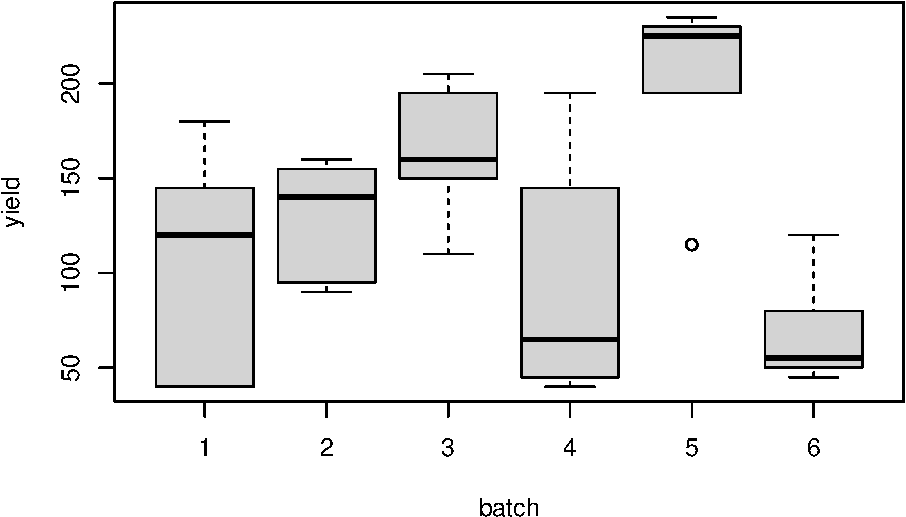
\includegraphics{bookdown_math3014-6027_files/figure-latex/napblack-summary-1} 

   }

   \caption{Naphthalene black experiment: distributions of dye yields from the six batches.}\label{fig:napblack-summary}
   \end{figure}

  Notice that even within any particular batch, the number of grams of standard dyestuff colour determined by the dye trial varies from observation to observation. This \emph{within-group} variation is considered to be random or residual variation. This cannot be explained by any differences between batches. However, a second source of variation in the overall data set can be explained by variation between the batches, i.e.~between the different batch means themselves. We can see from the box plots (Figure \ref{fig:napblack-summary}) and the mean yields in each batch that observations from batch number five appear to have given higher yields (in grams of standard colour) than those from the other batches.
\item
  When we fit linear models and compare them using analysis of variance (ANOVA), it enables us to decide whether the differences that seem to be evident in these simple plots and descriptive statistics are statistically significant or whether this kind of variation could have arisen by chance, even though there are no real differences between the batches.

  An ANOVA table may be used to compare a linear model including differences between the batches to the null model. The linear model we will fit is a simple unit-treatment model:

  \begin{equation}
   Y_{ij} =  \mu +  \tau_i +  \varepsilon_{ij} \,,\qquad i=1,\ldots,6;~j=1,\ldots,5\,,
   \label{eq:linmod}
   \end{equation}

  where \(Y_{ij}\) is the response obtained from the \(j\)th repetition of the \(i\)th batch, \(\mu\) is a constant term, \(\tau_i\) is the expected effect due to the observation being in the \(k\)th batch \((k=1,\ldots,5)\) and \(\varepsilon_{ij}\) are the random errors.

  A test of the hypothesis that the group means are all equal is equivalent to a test that the \(\tau_i\) are all equal to 0 \((H_0:\, \tau_1 = \tau_2 = \cdots = \tau_6 = 0)\). We can use \texttt{lm} to fit model \eqref{eq:linmod}, and \texttt{anova} to test the hypothesis. Before we fit the linear model, we need to make sure \texttt{batch} has type \texttt{factor}\footnote{Factors are variables in \texttt{R} which take on a limited number of different values (e.g.~categorical variables). We need to define a categorical variable, like \texttt{batch} as a \texttt{factor} to ensure they are treated correctly by functions such as \texttt{lm}.}.

\begin{Shaded}
\begin{Highlighting}[]
\NormalTok{napblack}\SpecialCharTok{$}\NormalTok{batch }\OtherTok{\textless{}{-}} \FunctionTok{as.factor}\NormalTok{(napblack}\SpecialCharTok{$}\NormalTok{batch)}
\NormalTok{napblack.lm }\OtherTok{\textless{}{-}} \FunctionTok{lm}\NormalTok{(yield }\SpecialCharTok{\textasciitilde{}}\NormalTok{ batch, }\AttributeTok{data =}\NormalTok{ napblack)}
\FunctionTok{anova}\NormalTok{(napblack.lm)}
\end{Highlighting}
\end{Shaded}

\begin{verbatim}
## Analysis of Variance Table
## 
## Response: yield
##           Df Sum Sq Mean Sq F value Pr(>F)   
## batch      5  56358   11272     4.6 0.0044 **
## Residuals 24  58830    2451                  
## ---
## Signif. codes:  0 '***' 0.001 '**' 0.01 '*' 0.05 '.' 0.1 ' ' 1
\end{verbatim}

  The p-value of 0.0044 indicates significant differences between at least two of the batch
  means. Therefore \(H_0\) is rejected and a suitable multiple comparison test should be carried
  out.
\item
  To perform our analysis, we have fitted a linear model. Therefore, we should use some plots of the residuals \(y_{ij} - \hat{y}_{ij}\) to check the model assumptions, particularly that the errors are independently and identically normally distributed. The function \texttt{rstandard} which produces residuals which have been standardised to have variance equal to 1.

\begin{Shaded}
\begin{Highlighting}[]
\NormalTok{standres }\OtherTok{\textless{}{-}} \FunctionTok{rstandard}\NormalTok{(napblack.lm)}
\NormalTok{fitted }\OtherTok{\textless{}{-}} \FunctionTok{fitted}\NormalTok{(napblack.lm)}
\FunctionTok{par}\NormalTok{(}\AttributeTok{mfrow =} \FunctionTok{c}\NormalTok{(}\DecValTok{1}\NormalTok{, }\DecValTok{2}\NormalTok{), }\AttributeTok{pty =} \StringTok{"s"}\NormalTok{)}
\FunctionTok{with}\NormalTok{(napblack, \{}
  \FunctionTok{plot}\NormalTok{(batch, standres, }\AttributeTok{xlab =} \StringTok{"Batch"}\NormalTok{, }\AttributeTok{ylab =} \StringTok{"Standarised residuals"}\NormalTok{)}
  \FunctionTok{plot}\NormalTok{(fitted, standres, }\AttributeTok{xlab =} \StringTok{"Fitted value"}\NormalTok{, }\AttributeTok{ylab =} \StringTok{"Standarised residuals"}\NormalTok{)}
\NormalTok{\})}
\end{Highlighting}
\end{Shaded}

  \begin{figure}

   {\centering 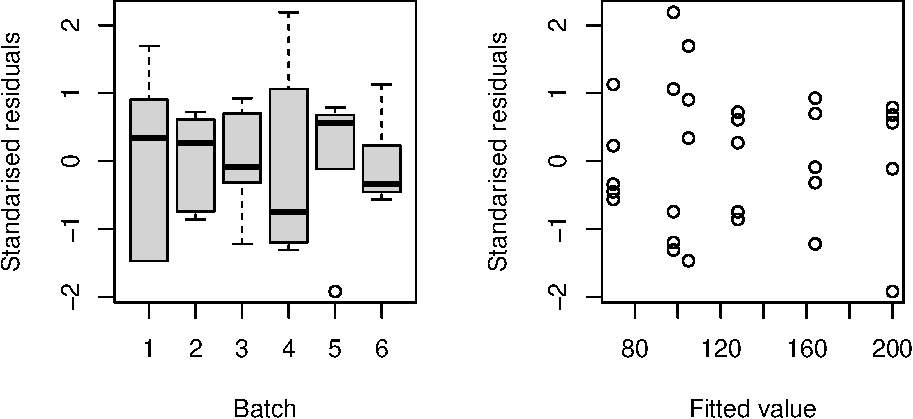
\includegraphics[width=1\linewidth]{bookdown_math3014-6027_files/figure-latex/residuals-1} 

   }

   \caption{Residuals against batch (left) and fitted values (right) for the linear model fit to the naphthalene black data.}\label{fig:residuals}
   \end{figure}

  The plots (Figure \ref{fig:residuals}) show no large standardised residuals (\(>2\) in absolute value\footnote{We would anticipate 95\% of the standardised residuals to lie in {[}-1.96, 1.96{]}, as they will follow a standard normal distribution if the model assumptions are correct.}). While there is some evidence of unequal variation across batches, there is no obvious pattern with respect to fitted values (e.g.~no ``funnelling'').

  We can also plot the standardised residuals against the quantiles of a standard normal distribution to assess the assumption of normality.

\begin{Shaded}
\begin{Highlighting}[]
\FunctionTok{par}\NormalTok{(}\AttributeTok{pty =} \StringTok{"s"}\NormalTok{)}
\FunctionTok{qqnorm}\NormalTok{(standres, }\AttributeTok{main =} \StringTok{""}\NormalTok{)}
\end{Highlighting}
\end{Shaded}

  \begin{figure}

   {\centering 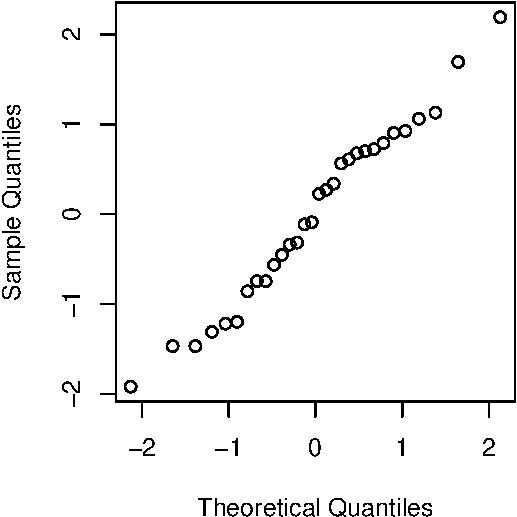
\includegraphics[width=1\linewidth]{bookdown_math3014-6027_files/figure-latex/normalplot-1} 

   }

   \caption{Normal probability plot for the standardised residuals for the linear model fit to the naphthalene black data.}\label{fig:normalplot}
   \end{figure}

  The points lie quite well on a straight line (see Figure \ref{fig:normalplot}), suggesting the assumption of normality is valid. Overall, the residual plots look reasonable; some investigation of transformations to correct for non-constant variance could be investigated (see MATH2010/STAT6123).
\item
  When a significant difference between the treatments has been indicated, the next stage is to try to determine which treatments differ. In some cases a specific difference is of interest, a control versus a new treatment for instance, in which case that difference could now be
  inspected. However, usually no specific differences are to be considered a priori, and \textit{any}
  difference is of practical importance. A multiple comparison procedure is required to
  investigate all possible differences, which takes account of the number of possible differences
  available amongst the treatments (15 differences between the six batches here).

  We will use Tukey's method for controlling the experiment-wise type I error rate, fixed here at 5\%, as implemented by \texttt{emmeans}.

\begin{Shaded}
\begin{Highlighting}[]
\NormalTok{napblack.emm }\OtherTok{\textless{}{-}}\NormalTok{ emmeans}\SpecialCharTok{::}\FunctionTok{emmeans}\NormalTok{(napblack.lm, }\StringTok{\textquotesingle{}batch\textquotesingle{}}\NormalTok{)}
\FunctionTok{pairs}\NormalTok{(napblack.emm)}
\end{Highlighting}
\end{Shaded}

\begin{verbatim}
##  contrast estimate   SE df t.ratio p.value
##  1 - 2         -23 31.3 24  -0.735  0.9755
##  1 - 3         -59 31.3 24  -1.884  0.4351
##  1 - 4           7 31.3 24   0.224  0.9999
##  1 - 5         -95 31.3 24  -3.034  0.0566
##  1 - 6          35 31.3 24   1.118  0.8692
##  2 - 3         -36 31.3 24  -1.150  0.8555
##  2 - 4          30 31.3 24   0.958  0.9266
##  2 - 5         -72 31.3 24  -2.299  0.2329
##  2 - 6          58 31.3 24   1.852  0.4535
##  3 - 4          66 31.3 24   2.108  0.3167
##  3 - 5         -36 31.3 24  -1.150  0.8555
##  3 - 6          94 31.3 24   3.002  0.0606
##  4 - 5        -102 31.3 24  -3.257  0.0348
##  4 - 6          28 31.3 24   0.894  0.9442
##  5 - 6         130 31.3 24   4.152  0.0043
## 
## P value adjustment: tukey method for comparing a family of 6 estimates
\end{verbatim}

  We have two significant differences, between batches 4-5 and 5-6.

\begin{Shaded}
\begin{Highlighting}[]
\FunctionTok{subset}\NormalTok{(}\FunctionTok{transform}\NormalTok{(}\FunctionTok{pairs}\NormalTok{(napblack.emm)), p.value }\SpecialCharTok{\textless{}} \FloatTok{0.05}\NormalTok{)}
\end{Highlighting}
\end{Shaded}

\begin{verbatim}
##    contrast estimate    SE df t.ratio  p.value
## 13    4 - 5     -102 31.31 24  -3.257 0.034820
## 15    5 - 6      130 31.31 24   4.152 0.004295
\end{verbatim}
\end{enumerate}

\begin{enumerate}
\def\labelenumi{\arabic{enumi}.}
\setcounter{enumi}{3}
\tightlist
\item
  \citep[Adapted from][]{Morris2011} Consider a completely randomised design with \(t = 5\) treatments and \(n=50\) units. The contrasts
\end{enumerate}

\[
\tau_2 - \tau_1, \quad \tau_3 - \tau_2, \quad \tau_4 - \tau_3, \tau_5 - \tau_4
\]

are of primary interest to the experimenter.

\begin{enumerate}
\def\labelenumi{\alph{enumi}.}
\item
  Find an allocation of the 50 units to the 5 treatments, i.e.~find \(n_1, \ldots, n_5\), that minimises the average variance of the corresponding contrast estimators.
\item
  Fixing the proportions of experimental effort applied to each treatment to those found in part (a), i.e.~to \(w_i = n_i/50\), find the value of \(n\) required to make the ratio \(T = |\boldsymbol{c}^{\mathrm{T}}\boldsymbol{\tau}|/\sqrt{\mbox{var}\left(\widehat{\boldsymbol{c}^{\mathrm{T}}\boldsymbol{\tau}}\right)} = 2\) assuming a signal-to-noise ratio of 1.
\end{enumerate}

Solution

\begin{enumerate}
\def\labelenumi{\alph{enumi}.}
\item
  We can use the function \texttt{opt\_ni} given in Section \ref{crd-opt-all}:

\begin{Shaded}
\begin{Highlighting}[]
\NormalTok{n }\OtherTok{\textless{}{-}} \DecValTok{50}
\NormalTok{C }\OtherTok{\textless{}{-}} \FunctionTok{matrix}\NormalTok{(}
  \FunctionTok{c}\NormalTok{(}
  \SpecialCharTok{{-}}\DecValTok{1}\NormalTok{, }\DecValTok{1}\NormalTok{, }\DecValTok{0}\NormalTok{, }\DecValTok{0}\NormalTok{, }\DecValTok{0}\NormalTok{,}
  \DecValTok{0}\NormalTok{, }\SpecialCharTok{{-}}\DecValTok{1}\NormalTok{, }\DecValTok{1}\NormalTok{, }\DecValTok{0}\NormalTok{, }\DecValTok{0}\NormalTok{,}
  \DecValTok{0}\NormalTok{, }\DecValTok{0}\NormalTok{, }\SpecialCharTok{{-}}\DecValTok{1}\NormalTok{, }\DecValTok{1}\NormalTok{, }\DecValTok{0}\NormalTok{,}
  \DecValTok{0}\NormalTok{, }\DecValTok{0}\NormalTok{, }\DecValTok{0}\NormalTok{, }\SpecialCharTok{{-}}\DecValTok{1}\NormalTok{, }\DecValTok{1}
\NormalTok{  ), }\AttributeTok{nrow =} \DecValTok{4}\NormalTok{, }\AttributeTok{byrow =}\NormalTok{ T}
\NormalTok{)}
\FunctionTok{opt\_ni}\NormalTok{(C, n) }
\end{Highlighting}
\end{Shaded}

\begin{verbatim}
## [1]  8.009 11.327 11.327 11.327  8.009
\end{verbatim}

  Rounding, we obtain a solution of the form \(n_1 = n_5 =8\), \(n_2 = n_4 = 11\) and \(n_3 = 12\). Any of \(n_2, n_3, n_4\) may be rounded up to 12 to form a design with the same variance.

\begin{Shaded}
\begin{Highlighting}[]
\NormalTok{nv }\OtherTok{\textless{}{-}} \FunctionTok{c}\NormalTok{(}\DecValTok{8}\NormalTok{, }\DecValTok{11}\NormalTok{, }\DecValTok{11}\NormalTok{, }\DecValTok{11}\NormalTok{, }\DecValTok{8}\NormalTok{)}
\FunctionTok{crd\_var}\NormalTok{(C, nv }\SpecialCharTok{+} \FunctionTok{c}\NormalTok{(}\DecValTok{0}\NormalTok{, }\DecValTok{1}\NormalTok{, }\DecValTok{0}\NormalTok{, }\DecValTok{0}\NormalTok{, }\DecValTok{0}\NormalTok{))}
\FunctionTok{crd\_var}\NormalTok{(C, nv }\SpecialCharTok{+} \FunctionTok{c}\NormalTok{(}\DecValTok{0}\NormalTok{, }\DecValTok{0}\NormalTok{, }\DecValTok{1}\NormalTok{, }\DecValTok{0}\NormalTok{, }\DecValTok{0}\NormalTok{))}
\FunctionTok{crd\_var}\NormalTok{(C, nv }\SpecialCharTok{+} \FunctionTok{c}\NormalTok{(}\DecValTok{0}\NormalTok{, }\DecValTok{0}\NormalTok{, }\DecValTok{0}\NormalTok{, }\DecValTok{1}\NormalTok{, }\DecValTok{0}\NormalTok{))}
\end{Highlighting}
\end{Shaded}

\begin{verbatim}
## [1] 0.7803
## [1] 0.7803
## [1] 0.7803
\end{verbatim}
\item
  The optimal ratios for each treatment from part (a) are \(w_1 = w_5 = 0.1602\) and \(w_2 = w_3 = w_4 = 0.2265\). Fixing these, we can use code from Section \ref{crd-size} to find the required value of \(n\) for each contrast.

\begin{Shaded}
\begin{Highlighting}[]
\NormalTok{nv }\OtherTok{\textless{}{-}} \ConstantTok{NULL}
\ControlFlowTok{for}\NormalTok{(i }\ControlFlowTok{in} \DecValTok{1}\SpecialCharTok{:}\DecValTok{4}\NormalTok{) nv[i] }\OtherTok{\textless{}{-}} \FunctionTok{opt\_n}\NormalTok{(C[i, ], }\FunctionTok{opt\_ni}\NormalTok{(C, n) }\SpecialCharTok{/}\NormalTok{ n, }\DecValTok{1}\NormalTok{, }\DecValTok{2}\NormalTok{) }\CommentTok{\# snr = 1, target = 2}
\NormalTok{nv}
\end{Highlighting}
\end{Shaded}

\begin{verbatim}
## [1] 42.63 35.31 35.31 42.63
\end{verbatim}

  Hence, we need \(n = 43\) for to achieve \(T = 2\) for the first and last contrasts, and \(n = 36\) for the second and third. The differences are due to the different proportions \(w_i\) assumed for each treatment. To achieve \(T=2\) for all contrasts, we pick the larger number, \(n = 43\).
\end{enumerate}

\hypertarget{blocking}{%
\chapter{Blocking}\label{blocking}}

The completely randomised design (CRD) works well when there is sufficient homogeneous experimental units to perform the whole experiment under the same, or very similar, conditions and there are no restrictions on the randomisation of treatments to units. The only systematic (non-random) differences in the observed responses result from differences between the treatments. While such designs are commonly and successfully used, especially in smaller experiments, their application can often be unrealistic or impractical in many settings.

A common way in which the CRD fails is a lack of sufficiently similar experimental units. If there are systemtic differences between different batches, or \textbf{blocks} of units, these differences should be taken into account in both the allocation of treatments to units and the modelling of the resultant data. Otherwise, block-to-block differences may bias treatment comparisons and/or inflate our estimate of the background variability and hence reduce our ability to detect important treatment effects.

\begin{example}
\protect\hypertarget{exm:blocks-bars}{}\label{exm:blocks-bars}

Steel bar experiment \citep[ch.~4]{Morris2011}

\citet{KSN2005} described an experiment to assess the strength of steel reinforcement bars from \(t=4\) coatings\footnote{The four coatings were all made from Engineering Thermoplastic Polyurethane (ETPU); coating one was solely made from ETPU, coatings 2-4 had additional glass fibre, carbon fibre or aramid fibre added, respectively.} (treatments). In total \(n=32\) different bars (units) were available, but the testing process meant sets of four bars were tested together. To account for potential test-specific features (e.g.~environmental or operational), these different test sets were assumed to form \(b=8\) blocks of size \(k=4\). The data are shown in Table \ref{tab:bar-expt-data} below.

\begin{Shaded}
\begin{Highlighting}[]
\NormalTok{bar }\OtherTok{\textless{}{-}} \FunctionTok{data.frame}\NormalTok{(}\AttributeTok{coating =} \FunctionTok{rep}\NormalTok{(}\FunctionTok{factor}\NormalTok{(}\DecValTok{1}\SpecialCharTok{:}\DecValTok{4}\NormalTok{), }\DecValTok{8}\NormalTok{),}
                   \AttributeTok{block =} \FunctionTok{rep}\NormalTok{(}\FunctionTok{factor}\NormalTok{(}\DecValTok{1}\SpecialCharTok{:}\DecValTok{8}\NormalTok{), }\FunctionTok{rep}\NormalTok{(}\DecValTok{4}\NormalTok{, }\DecValTok{8}\NormalTok{)), }
                   \AttributeTok{strength =} \FunctionTok{c}\NormalTok{(}\DecValTok{136}\NormalTok{, }\DecValTok{147}\NormalTok{, }\DecValTok{138}\NormalTok{, }\DecValTok{149}\NormalTok{, }\DecValTok{136}\NormalTok{, }\DecValTok{143}\NormalTok{, }\DecValTok{122}\NormalTok{, }\DecValTok{153}\NormalTok{, }\DecValTok{150}\NormalTok{, }\DecValTok{142}\NormalTok{, }\DecValTok{131}\NormalTok{, }\DecValTok{136}\NormalTok{,}
                                   \DecValTok{155}\NormalTok{, }\DecValTok{148}\NormalTok{, }\DecValTok{130}\NormalTok{, }\DecValTok{129}\NormalTok{, }\DecValTok{145}\NormalTok{, }\DecValTok{149}\NormalTok{, }\DecValTok{136}\NormalTok{, }\DecValTok{139}\NormalTok{, }\DecValTok{150}\NormalTok{, }\DecValTok{149}\NormalTok{, }\DecValTok{147}\NormalTok{, }\DecValTok{144}\NormalTok{,}
                                   \DecValTok{147}\NormalTok{, }\DecValTok{150}\NormalTok{, }\DecValTok{125}\NormalTok{, }\DecValTok{140}\NormalTok{, }\DecValTok{148}\NormalTok{, }\DecValTok{149}\NormalTok{, }\DecValTok{118}\NormalTok{, }\DecValTok{145}\NormalTok{)}
\NormalTok{                     )}
\NormalTok{knitr}\SpecialCharTok{::}\FunctionTok{kable}\NormalTok{(}
\NormalTok{ tidyr}\SpecialCharTok{::}\FunctionTok{pivot\_wider}\NormalTok{(bar, }\AttributeTok{names\_from =}\NormalTok{ coating, }\AttributeTok{values\_from =}\NormalTok{ strength),}
 \AttributeTok{col.names =} \FunctionTok{c}\NormalTok{(}\StringTok{"Block"}\NormalTok{, }\FunctionTok{paste}\NormalTok{(}\StringTok{"Coating"}\NormalTok{, }\DecValTok{1}\SpecialCharTok{:}\DecValTok{4}\NormalTok{)),}
 \AttributeTok{caption =} \StringTok{"Steel bar experiment: tensile strength values (kliograms per square inch, ksi) from steel bars with four different coatings."}
\NormalTok{)}
\end{Highlighting}
\end{Shaded}

\begin{table}

\caption{\label{tab:bar-expt-data}Steel bar experiment: tensile strength values (kliograms per square inch, ksi) from steel bars with four different coatings.}
\centering
\begin{tabular}[t]{l|r|r|r|r}
\hline
Block & Coating 1 & Coating 2 & Coating 3 & Coating 4\\
\hline
1 & 136 & 147 & 138 & 149\\
\hline
2 & 136 & 143 & 122 & 153\\
\hline
3 & 150 & 142 & 131 & 136\\
\hline
4 & 155 & 148 & 130 & 129\\
\hline
5 & 145 & 149 & 136 & 139\\
\hline
6 & 150 & 149 & 147 & 144\\
\hline
7 & 147 & 150 & 125 & 140\\
\hline
8 & 148 & 149 & 118 & 145\\
\hline
\end{tabular}
\end{table}

Here, each block has size 4, which is equal to the number of treatments in the experiment, and each treatment is applied in each block. This is an example of a \textbf{randomised complete block design}.

We can study the data graphically, plotting by treatment and by block.

\begin{Shaded}
\begin{Highlighting}[]
\FunctionTok{boxplot}\NormalTok{(strength }\SpecialCharTok{\textasciitilde{}}\NormalTok{ block, }\AttributeTok{data =}\NormalTok{ bar)}
\FunctionTok{boxplot}\NormalTok{(strength }\SpecialCharTok{\textasciitilde{}}\NormalTok{ coating, }\AttributeTok{data =}\NormalTok{ bar)}
\end{Highlighting}
\end{Shaded}

\begin{figure}

{\centering 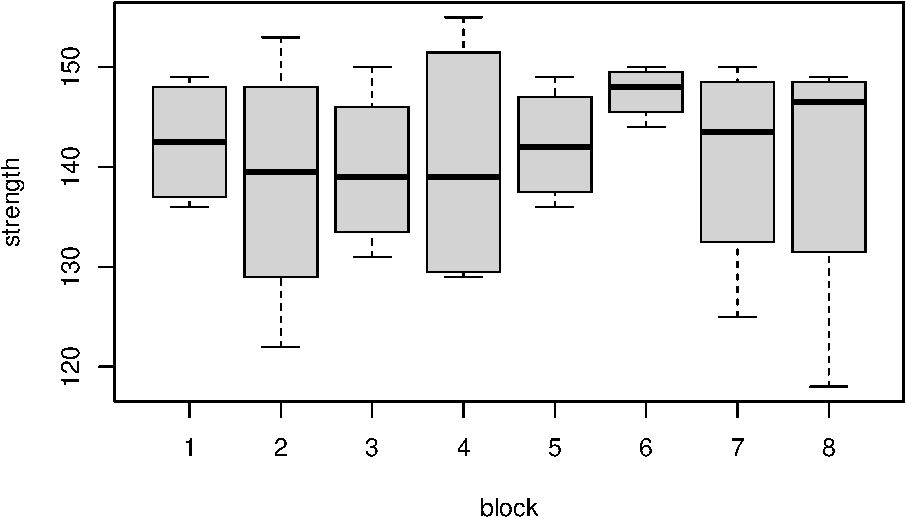
\includegraphics{bookdown_math3014-6027_files/figure-latex/bar-expt-boxplots-1} 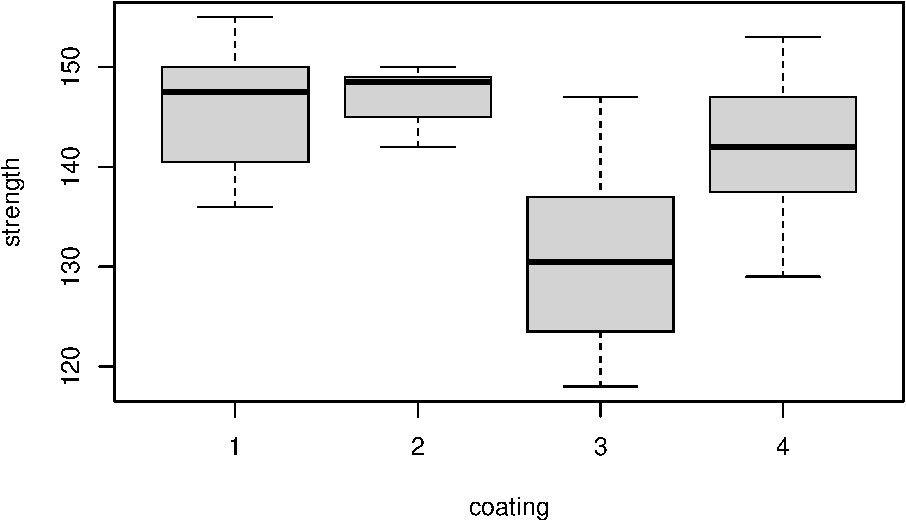
\includegraphics{bookdown_math3014-6027_files/figure-latex/bar-expt-boxplots-2} 

}

\caption{Steel bar experiment: distributions of tensile strength (ksi) from the eight blocks (top) and the four coatings (bottom).}\label{fig:bar-expt-boxplots}
\end{figure}

The box plots within each plot in Figure \ref{fig:bar-expt-boxplots} are comparable, as every treatment has occured with every block the same number of times (once). For example, when we compare the box plots for treatments 1 and 3, we know each of then display one observation from each block. Therefore, differences between treatments will not be influenced by large differences between blocks. This \textbf{balance} makes our analysis more straighforward. By eye, it appears here there may be differences between both coating 3 and the other three coatings.

\end{example}

\begin{example}
\protect\hypertarget{exm:blocks-tyres}{}\label{exm:blocks-tyres}

Tyre experiment \citep[ch.~3]{WH2009}

\citet{Davies1954}, p.200, examined the effect of \(t=4\) different rubber compounds (treatments) on the lifetime of a tyre. Each tyre is only large enough to split into \(k=3\) segments whilst still containing a representative amount of each compound. When tested, each tyre is subjected to the same road conditions, and hence is treated as a block. A design with \(b=4\) blocks was used, as displayed in Table \ref{tab:tyre-expt-data}.

\begin{Shaded}
\begin{Highlighting}[]
\NormalTok{tyre }\OtherTok{\textless{}{-}} \FunctionTok{data.frame}\NormalTok{(}\AttributeTok{compound =} \FunctionTok{as.factor}\NormalTok{(}\FunctionTok{c}\NormalTok{(}\DecValTok{1}\NormalTok{, }\DecValTok{2}\NormalTok{, }\DecValTok{3}\NormalTok{, }\DecValTok{1}\NormalTok{, }\DecValTok{2}\NormalTok{, }\DecValTok{4}\NormalTok{, }\DecValTok{1}\NormalTok{, }\DecValTok{3}\NormalTok{, }\DecValTok{4}\NormalTok{, }\DecValTok{2}\NormalTok{, }\DecValTok{3}\NormalTok{, }\DecValTok{4}\NormalTok{)),}
                   \AttributeTok{block =} \FunctionTok{rep}\NormalTok{(}\FunctionTok{factor}\NormalTok{(}\DecValTok{1}\SpecialCharTok{:}\DecValTok{4}\NormalTok{), }\FunctionTok{rep}\NormalTok{(}\DecValTok{3}\NormalTok{, }\DecValTok{4}\NormalTok{)), }
                   \AttributeTok{wear =} \FunctionTok{c}\NormalTok{(}\DecValTok{238}\NormalTok{, }\DecValTok{238}\NormalTok{, }\DecValTok{279}\NormalTok{, }\DecValTok{196}\NormalTok{, }\DecValTok{213}\NormalTok{, }\DecValTok{308}\NormalTok{, }\DecValTok{254}\NormalTok{, }\DecValTok{334}\NormalTok{, }\DecValTok{367}\NormalTok{, }\DecValTok{312}\NormalTok{, }\DecValTok{421}\NormalTok{, }\DecValTok{412}\NormalTok{)}
\NormalTok{                     )}
\FunctionTok{options}\NormalTok{(}\AttributeTok{knitr.kable.NA =} \StringTok{\textquotesingle{}\textquotesingle{}}\NormalTok{)}
\NormalTok{knitr}\SpecialCharTok{::}\FunctionTok{kable}\NormalTok{(}
\NormalTok{ tidyr}\SpecialCharTok{::}\FunctionTok{pivot\_wider}\NormalTok{(tyre, }\AttributeTok{names\_from =}\NormalTok{ compound, }\AttributeTok{values\_from =}\NormalTok{ wear),}
 \AttributeTok{col.names =} \FunctionTok{c}\NormalTok{(}\StringTok{"Block"}\NormalTok{, }\FunctionTok{paste}\NormalTok{(}\StringTok{"Compound"}\NormalTok{, }\DecValTok{1}\SpecialCharTok{:}\DecValTok{4}\NormalTok{)),}
 \AttributeTok{caption =} \StringTok{"Tyre experiment: relative wear measurements (unitless) from tires made with four different rubber compounds."}
\NormalTok{)}
\end{Highlighting}
\end{Shaded}

\begin{table}

\caption{\label{tab:tyre-expt-data}Tyre experiment: relative wear measurements (unitless) from tires made with four different rubber compounds.}
\centering
\begin{tabular}[t]{l|r|r|r|r}
\hline
Block & Compound 1 & Compound 2 & Compound 3 & Compound 4\\
\hline
1 & 238 & 238 & 279 & \\
\hline
2 & 196 & 213 &  & 308\\
\hline
3 & 254 &  & 334 & 367\\
\hline
4 &  & 312 & 421 & 412\\
\hline
\end{tabular}
\end{table}

Here, each block has size \(k=3\), which is smaller than the number of treatments (\(t=4\)). Hence, each block cannot contain an application of each treatment. This is an example of an \textbf{incomplete block design}.

Graphical exploration of the data is a little more problematic in this example. As each treatment does not occur in each block, box plots such as Figure \ref{fig:tyre-expt-boxplots} are not as informative. Do compounds three and four have higher average wear because they were the only compounds to both occur in blocks 3 and 4? Or do blocks 3 and 4 have a higher mean because they contain both compounds 3 and 4? The design cannot help us entirely disentangle the impact of blocks and treatments\footnote{This is our first example of (partial) confounding, which we will see again in Chapters \ref{block-factorial} and \ref{fractional-factorial}}. In our modelling, we will assume variation should first be described by blocks (which are generally fixed aspects of the experiment) and then treatments (which are more directly under the experimenter's control).

\begin{Shaded}
\begin{Highlighting}[]
\FunctionTok{boxplot}\NormalTok{(wear }\SpecialCharTok{\textasciitilde{}}\NormalTok{ block, }\AttributeTok{data =}\NormalTok{ tyre)}
\FunctionTok{boxplot}\NormalTok{(wear }\SpecialCharTok{\textasciitilde{}}\NormalTok{ compound, }\AttributeTok{data =}\NormalTok{ tyre)}
\end{Highlighting}
\end{Shaded}

\begin{figure}

{\centering 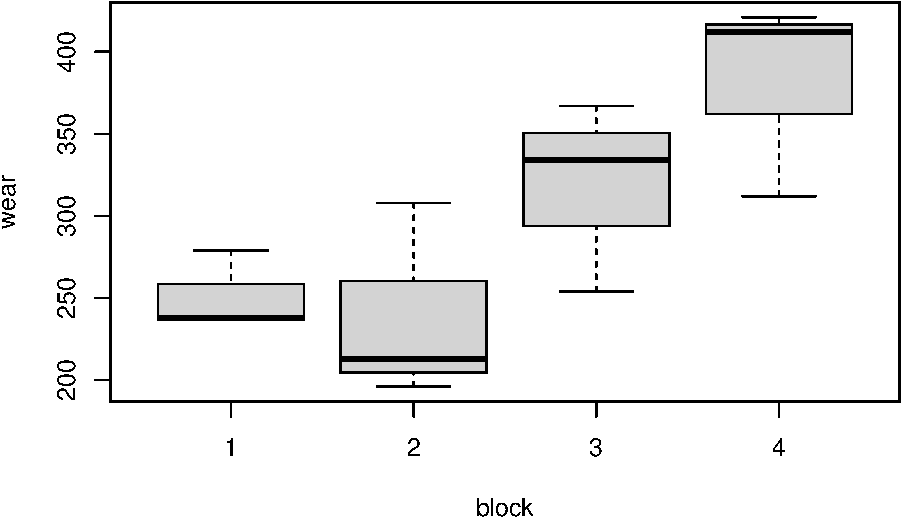
\includegraphics{bookdown_math3014-6027_files/figure-latex/tyre-expt-boxplots-1} 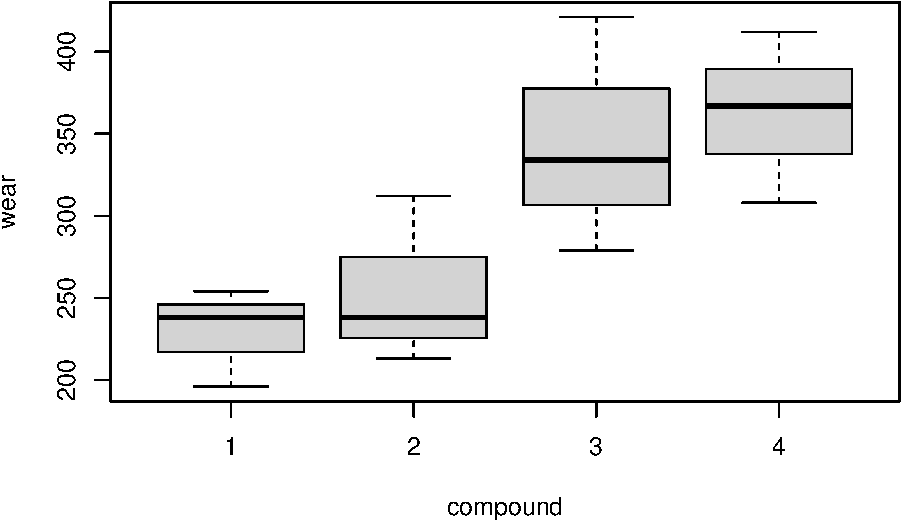
\includegraphics{bookdown_math3014-6027_files/figure-latex/tyre-expt-boxplots-2} 

}

\caption{Tyre experiment: distributions of wear from the four blocks (top) and the four compounds (bottom).}\label{fig:tyre-expt-boxplots}
\end{figure}

\end{example}

\hypertarget{unit-block-treatment-model}{%
\section{Unit-block-treatment model}\label{unit-block-treatment-model}}

If \(n_{ij}\) is the number of times treatment \(j\) occurs in block \(i\), a common statistical model to describe data from a blocked experiment has the form

\begin{equation}
y_{ijl} = \mu + \beta_i + \tau_j + \varepsilon_{ijl}\,, \qquad i = 1,\ldots, b; j = 1, \ldots, t; l = 1,\ldots,n_{ij}\,,
\label{eq:block-model}
\end{equation}
where \(y_{ijl}\) is the response from the \(l\)th application of the \(j\)th treatment in the \(i\)th block, \(\mu\) is a constant parameter, \(\beta_i\) is the effect of the \(i\)th block, \(\tau_j\) is the effect of treatment \(j\), and \(\varepsilon_{ijl}\sim N(0, \sigma^2)\) are once again random individual effects from each experimental unit, assumed independent. The total number of runs in the experiment is given by \(n = \sum_{i=1}^b\sum_{j=1}^t n_{ij}\).

For Example \ref{exm:blocks-bars}, there are \(t=4\) experiments, \(b = 8\) blocks and each treatment occurs once in each block, so \(n_{ij} = 1\) for all \(i, j\). In Example \ref{exm:blocks-tyres}, there are again \(t=4\) treatments but now only \(b=4\) blocks and not every treatment occurs in every block. In fact, we have \(n_{11} = n_{12} = n_{13} = 1\), \(n_{14} = 0\), \(n_{21} = n_{22} =n_{24} = 1\), \(n_{23} = 0\), \(n_{31} = n_{33} =n_{34} = 1\), \(n_{32} = 0\), \(n_{41} = 0\) and \(n_{42} = n_{43} =n_{44} = 1\).

Writing model \eqref{eq:block-model} is matrix form as a partitioned linear model, we obtain

\begin{equation}
\boldsymbol{y}= \mu\boldsymbol{1}_n + X_1\boldsymbol{\beta} + X_2\boldsymbol{\tau} + \boldsymbol{\varepsilon}\,,
\label{eq:block-plm}
\end{equation}

with \(\boldsymbol{y}\) the \(n\)-vector of responses, \(X_1\) and \(X_2\) \(n\times b\) and \(n\times t\) model matrices for blocks and treatments, respectively, \(\boldsymbol{\beta} = (\beta_1,\ldots, \beta_b)^{\mathrm{T}}\), \(\boldsymbol{\tau} = (\tau_1,\ldots, \tau_t)^{\mathrm{T}}\) and \(\boldsymbol{\varepsilon}\) the \(n\)-vector of errors.

In equation\eqref{eq:block-plm}, assuming without loss of generality that runs of the experiment are ordered by block, the matrix \(X_1\) has the form

\[
X_1 = \bigoplus_{i = 1}^b \boldsymbol{1}_{k_i} = \begin{bmatrix}
\boldsymbol{1}_{k_1} & \boldsymbol{0}_{k_1} & \cdots &  \boldsymbol{0}_{k_1} \\
\boldsymbol{0}_{k_2} & \boldsymbol{1}_{k_2} & \cdots &  \boldsymbol{0}_{k_2} \\
\vdots & & \ddots & \vdots \\
\boldsymbol{0}_{k_b} & \boldsymbol{0}_{k_b} & \cdots &  \boldsymbol{1}_{k_b} \\
\end{bmatrix}\,,
\]
where \(k_i = \sum_{j=1}^t n_{ij}\), the number of units in the \(i\)th block. The structure of matrix \(X_2\) is harder to describe so distinctly, but each row includes a single non-zero entry, equal to one, indicating which treatment was applied in that run of the experiment. The first \(k_1\) rows correspond to block 1, the second \(k_2\) to block 2, and so on. We will see special cases later.

\hypertarget{normal-equations}{%
\section{Normal equations}\label{normal-equations}}

Writing as a partitioned model \(\boldsymbol{y}= W\boldsymbol{\alpha} + \boldsymbol{\varepsilon}\), with \(W = [\boldsymbol{1} | X_1 | X_2]\) and \(\boldsymbol{\alpha}^{\mathrm{T}} = [\mu | \boldsymbol{\beta}^{\mathrm{T}} | \boldsymbol{\tau}^{\mathrm{T}}]\), the least squares normal equations

\begin{equation}
W^{\mathrm{T}}W \hat{\boldsymbol{\alpha}} = W^{\mathrm{T}}\boldsymbol{y}
\label{eq:bne}
\end{equation}

can be written as a set of three matrix equations:

\begin{align}
n\hat{\mu} + \boldsymbol{1}_n^{\mathrm{T}}X_1\hat{\boldsymbol{\beta}} + \boldsymbol{1}_n^{\mathrm{T}}X_2\hat{\boldsymbol{\tau}} & = \boldsymbol{1}_n^{\mathrm{T}}\boldsymbol{y}\,, \label{eq:blocks-normal-1}\\
X_1^{\mathrm{T}}\boldsymbol{1}_n\hat{\mu} + X_1^{\mathrm{T}}X_1\hat{\boldsymbol{\beta}} + X_1^{\mathrm{T}}X_2\hat{\boldsymbol{\tau}} & = X_1^{\mathrm{T}}\boldsymbol{y}\,, \label{eq:blocks-normal-2}\\
X_2^{\mathrm{T}}\boldsymbol{1}_n\hat{\mu} + X_2^{\mathrm{T}}X_1\hat{\boldsymbol{\beta}} + X_2^{\mathrm{T}}X_2\hat{\boldsymbol{\tau}} & = X_2^{\mathrm{T}}\boldsymbol{y}\,. \label{eq:blocks-normal-3}\\
\end{align}

Above, the matrices \(X_1^{\mathrm{T}}X_1 = \mathrm{diag}(k_1,\ldots,k_b)\) and \(X_2^{\mathrm{T}}X_2 = \mathrm{diag}(n_1,\ldots,n_t)\) have simple forms as diagonal matrices with entries equal to the size of each block and the number of replications of each treatment, respectively.

The \(t\times b\) matrix \(N = X_2^{\mathcal{T}}X_1\) is particularly important in block designs, and is called the \textbf{incidence} matrix. Each of the \(i\)th row of \(N\) indicates in which blocks the \(i\)th treatment occurs.

We can eliminate the explicit dependence on \(\mu\) and \(\boldsymbol{\beta}\) to find reduced normal equations for \(\boldsymbol{\tau}\) by multiplying the middle equation by \(X_2^{\mathrm{T}}X_1(X_1^{\mathrm{T}}X_1)^{-1}\):

\begin{multline}
X_2^{\mathrm{T}}X_1(X_1^{\mathrm{T}}X_1)^{-1}X_1^{\mathrm{T}}\boldsymbol{1}_n\hat{\mu} + X_2^{\mathrm{T}}X_1(X_1^{\mathrm{T}}X_1)^{-1}X_1^{\mathrm{T}}X_1\hat{\boldsymbol{\beta}} + X_2^{\mathrm{T}}X_1(X_1^{\mathrm{T}}X_1)^{-1}X_1^{\mathrm{T}}X_2\hat{\boldsymbol{\tau}} \\
 = X_2^{\mathrm{T}}X_1(X_1^{\mathrm{T}}X_1)^{-1}X_1^{\mathrm{T}}\boldsymbol{1}_n\hat{\mu} + X_2^{\mathrm{T}}X_1\hat{\boldsymbol{\beta}} + X_2^{\mathrm{T}}X_1(X_1^{\mathrm{T}}X_1)^{-1}X_1^{\mathrm{T}}X_2\hat{\boldsymbol{\tau}} \\
 = X_2^{\mathrm{T}}X_1(X_1^{\mathrm{T}}X_1)^{-1}X_1^{\mathrm{T}}\boldsymbol{y}\\
\end{multline}

and subtracting from the final equation:

\begin{multline}
X_2^{\mathrm{T}}\left(\boldsymbol{1}_n - X_1(X_1^{\mathrm{T}}X_1)^{-1}X_1^{\mathrm{T}}\boldsymbol{1}_n\right)\hat{\mu} + \left(X_2^{\mathrm{T}}X_1 - X_2^{\mathrm{T}}X_1\right)\hat{\boldsymbol{\beta}} \\ + X_2^{\mathrm{T}}\left(I_n - X_1(X_1^{\mathrm{T}}X_1)^{-1}X_1^{\mathrm{T}}\right)X_2\hat{\boldsymbol{\tau}}\\
= X_2^{\mathrm{T}}\left(I_n - X_1(X_1^{\mathrm{T}}X_1)^{-1}X_1^{\mathrm{T}}\right)\boldsymbol{y}\,.
\end{multline}
Clearly, a zero matrix is multiplying the block effects \(\hat{\boldsymbol{\beta}}\). Also,

\[
X_1(X_1^{\mathrm{T}}X_1)^{-1}X_1^{\mathrm{T}}\boldsymbol{1}_n = \boldsymbol{1}_n\,,
\]
as

\[
X_1(X_1^{\mathrm{T}}X_1)^{-1} = \bigoplus_{i = 1}^b \frac{1}{k_i}\boldsymbol{1}_{k_i} = \begin{bmatrix}
\frac{1}{k_1}\boldsymbol{1}_{k_1} & \boldsymbol{0}_{k_1} & \cdots &  \boldsymbol{0}_{k_1} \\
\boldsymbol{0}_{k_2} & \frac{1}{k_2}\boldsymbol{1}_{k_2} & \cdots &  \boldsymbol{0}_{k_2} \\
\vdots & & \ddots & \vdots \\
\boldsymbol{0}_{k_b} & \boldsymbol{0}_{k_b} & \cdots &  \frac{1}{k_b}\boldsymbol{1}_{k_b} \\
\end{bmatrix}\,,
\]
and hence

\[
X_1(X_1^{\mathrm{T}}X_1)^{-1}X_1^{\mathrm{T}} = \bigoplus_{i = 1}^b \frac{1}{k_i}J_{k_i} = \begin{bmatrix}
\frac{1}{k_1}J_{k_1} & \boldsymbol{0}_{k_1\times k_2} & \cdots &  \boldsymbol{0}_{k_1\times k_b} \\
\boldsymbol{0}_{k_2\times k_1} & \frac{1}{k_2}J_{k_2} & \cdots &  \boldsymbol{0}_{k_2\times k_b} \\
\vdots & & \ddots & \vdots \\
\boldsymbol{0}_{k_b\times k_1} & \boldsymbol{0}_{k_b\times k_2} & \cdots &  \frac{1}{k_b}J_{k_b} \\
\end{bmatrix}\,.
\]

Writing \(H_1 = X_1(X_1^{\mathrm{T}}X_1)^{-1}X_1^{\mathrm{T}}\), we then get the reduced normal equations for \(\boldsymbol{\tau}\):

\begin{equation}
X_2^{\mathrm{T}}\left(I_n - H_1\right)X_2\hat{\boldsymbol{\tau}}= X_2^{\mathrm{T}}\left(I_n - H_1\right)\boldsymbol{y}\,.
\label{eq:block-rne}
\end{equation}

We can demonstrate the form of these matrices through our two examples.

For Example \ref{exm:blocks-bars}:

\begin{Shaded}
\begin{Highlighting}[]
\NormalTok{one }\OtherTok{\textless{}{-}} \FunctionTok{rep}\NormalTok{(}\DecValTok{1}\NormalTok{, }\DecValTok{4}\NormalTok{)}
\NormalTok{X1 }\OtherTok{\textless{}{-}} \FunctionTok{kronecker}\NormalTok{(}\FunctionTok{diag}\NormalTok{(}\DecValTok{1}\NormalTok{, }\AttributeTok{nrow =} \DecValTok{8}\NormalTok{), one)}
\NormalTok{X2 }\OtherTok{\textless{}{-}} \FunctionTok{diag}\NormalTok{(}\DecValTok{1}\NormalTok{, }\AttributeTok{nrow =} \DecValTok{4}\NormalTok{)}
\NormalTok{X2 }\OtherTok{\textless{}{-}} \FunctionTok{do.call}\NormalTok{(}\StringTok{"rbind"}\NormalTok{, }\FunctionTok{replicate}\NormalTok{(}\DecValTok{8}\NormalTok{, X2, }\AttributeTok{simplify =} \ConstantTok{FALSE}\NormalTok{))}
\CommentTok{\#incidence matrix}
\NormalTok{N }\OtherTok{\textless{}{-}} \FunctionTok{t}\NormalTok{(X2) }\SpecialCharTok{\%*\%}\NormalTok{ X1}
\NormalTok{X1tX1 }\OtherTok{\textless{}{-}} \FunctionTok{t}\NormalTok{(X1) }\SpecialCharTok{\%*\%}\NormalTok{ X1 }\CommentTok{\# diagonal}
\NormalTok{X2tX2 }\OtherTok{\textless{}{-}} \FunctionTok{t}\NormalTok{(X2) }\SpecialCharTok{\%*\%}\NormalTok{ X2 }\CommentTok{\# diagonal}
\NormalTok{H1 }\OtherTok{\textless{}{-}}\NormalTok{ X1 }\SpecialCharTok{\%*\%} \FunctionTok{solve}\NormalTok{(}\FunctionTok{t}\NormalTok{(X1) }\SpecialCharTok{\%*\%}\NormalTok{ X1) }\SpecialCharTok{\%*\%} \FunctionTok{t}\NormalTok{(X1)}
\NormalTok{ones }\OtherTok{\textless{}{-}}\NormalTok{ H1 }\SpecialCharTok{\%*\%} \FunctionTok{rep}\NormalTok{(}\DecValTok{1}\NormalTok{, }\DecValTok{32}\NormalTok{) }\CommentTok{\# H1 times vector of 1s is also a vector of 1s}
\NormalTok{A }\OtherTok{\textless{}{-}} \FunctionTok{t}\NormalTok{(X2) }\SpecialCharTok{\%*\%}\NormalTok{ X2 }\SpecialCharTok{{-}} \FunctionTok{t}\NormalTok{(X2) }\SpecialCharTok{\%*\%}\NormalTok{ H1 }\SpecialCharTok{\%*\%}\NormalTok{ X2 }\CommentTok{\# X2t(I {-} H1)X2}
\FunctionTok{qr}\NormalTok{(A)}\SpecialCharTok{$}\NormalTok{rank }\CommentTok{\# rank 3}
\NormalTok{X2tH1 }\OtherTok{\textless{}{-}} \FunctionTok{t}\NormalTok{(X2) }\SpecialCharTok{\%*\%}\NormalTok{ H1 }\CommentTok{\# adjustment to y}
\NormalTok{W }\OtherTok{\textless{}{-}} \FunctionTok{cbind}\NormalTok{(ones, X1, X2) }\CommentTok{\# overall model matrix}
\FunctionTok{qr}\NormalTok{(W)}\SpecialCharTok{$}\NormalTok{rank }\CommentTok{\# rank 11 (t+b {-} 1)}
\end{Highlighting}
\end{Shaded}

For Example \ref{exm:blocks-tyres}:

\begin{Shaded}
\begin{Highlighting}[]
\NormalTok{one }\OtherTok{\textless{}{-}} \FunctionTok{rep}\NormalTok{(}\DecValTok{1}\NormalTok{, }\DecValTok{3}\NormalTok{)}
\NormalTok{X1 }\OtherTok{\textless{}{-}} \FunctionTok{kronecker}\NormalTok{(}\FunctionTok{diag}\NormalTok{(}\DecValTok{1}\NormalTok{, }\AttributeTok{nrow =} \DecValTok{4}\NormalTok{), one)}
\NormalTok{X2 }\OtherTok{\textless{}{-}} \FunctionTok{matrix}\NormalTok{(}
        \FunctionTok{c}\NormalTok{(}\DecValTok{1}\NormalTok{, }\DecValTok{0}\NormalTok{, }\DecValTok{0}\NormalTok{, }\DecValTok{0}\NormalTok{,}
          \DecValTok{0}\NormalTok{, }\DecValTok{1}\NormalTok{, }\DecValTok{0}\NormalTok{, }\DecValTok{0}\NormalTok{,}
          \DecValTok{0}\NormalTok{, }\DecValTok{0}\NormalTok{, }\DecValTok{1}\NormalTok{, }\DecValTok{0}\NormalTok{,}
          \DecValTok{1}\NormalTok{, }\DecValTok{0}\NormalTok{, }\DecValTok{0}\NormalTok{, }\DecValTok{0}\NormalTok{,}
          \DecValTok{0}\NormalTok{, }\DecValTok{1}\NormalTok{, }\DecValTok{0}\NormalTok{, }\DecValTok{0}\NormalTok{,}
          \DecValTok{0}\NormalTok{, }\DecValTok{0}\NormalTok{, }\DecValTok{0}\NormalTok{, }\DecValTok{1}\NormalTok{,}
          \DecValTok{1}\NormalTok{, }\DecValTok{0}\NormalTok{, }\DecValTok{0}\NormalTok{, }\DecValTok{0}\NormalTok{,}
          \DecValTok{0}\NormalTok{, }\DecValTok{0}\NormalTok{, }\DecValTok{1}\NormalTok{, }\DecValTok{0}\NormalTok{,}
          \DecValTok{0}\NormalTok{, }\DecValTok{0}\NormalTok{, }\DecValTok{0}\NormalTok{, }\DecValTok{1}\NormalTok{,}
          \DecValTok{0}\NormalTok{, }\DecValTok{1}\NormalTok{, }\DecValTok{0}\NormalTok{, }\DecValTok{0}\NormalTok{,}
          \DecValTok{0}\NormalTok{, }\DecValTok{0}\NormalTok{, }\DecValTok{1}\NormalTok{, }\DecValTok{0}\NormalTok{,}
          \DecValTok{0}\NormalTok{, }\DecValTok{0}\NormalTok{, }\DecValTok{0}\NormalTok{, }\DecValTok{1}\NormalTok{), }\AttributeTok{nrow =} \DecValTok{12}\NormalTok{, }\AttributeTok{byrow =}\NormalTok{ T}
\NormalTok{)}
\CommentTok{\#incidence matrix}
\NormalTok{N }\OtherTok{\textless{}{-}} \FunctionTok{t}\NormalTok{(X2) }\SpecialCharTok{\%*\%}\NormalTok{ X1}
\NormalTok{X1tX1 }\OtherTok{\textless{}{-}} \FunctionTok{t}\NormalTok{(X1) }\SpecialCharTok{\%*\%}\NormalTok{ X1 }\CommentTok{\# diagonal}
\NormalTok{X2tX2 }\OtherTok{\textless{}{-}} \FunctionTok{t}\NormalTok{(X2) }\SpecialCharTok{\%*\%}\NormalTok{ X2 }\CommentTok{\# diagonal}
\NormalTok{H1 }\OtherTok{\textless{}{-}}\NormalTok{ X1 }\SpecialCharTok{\%*\%} \FunctionTok{solve}\NormalTok{(}\FunctionTok{t}\NormalTok{(X1) }\SpecialCharTok{\%*\%}\NormalTok{ X1) }\SpecialCharTok{\%*\%} \FunctionTok{t}\NormalTok{(X1)}
\NormalTok{ones }\OtherTok{\textless{}{-}}\NormalTok{ H1 }\SpecialCharTok{\%*\%} \FunctionTok{rep}\NormalTok{(}\DecValTok{1}\NormalTok{, }\DecValTok{12}\NormalTok{) }\CommentTok{\# H1 times vector of 1s is also a vector of 1s}
\NormalTok{A }\OtherTok{\textless{}{-}} \FunctionTok{t}\NormalTok{(X2) }\SpecialCharTok{\%*\%}\NormalTok{ X2 }\SpecialCharTok{{-}} \FunctionTok{t}\NormalTok{(X2) }\SpecialCharTok{\%*\%}\NormalTok{ H1 }\SpecialCharTok{\%*\%}\NormalTok{ X2 }\CommentTok{\# X2t(I {-} H1)X2}
\FunctionTok{qr}\NormalTok{(A)}\SpecialCharTok{$}\NormalTok{rank }\CommentTok{\# rank 3}
\NormalTok{X2tH1 }\OtherTok{\textless{}{-}} \FunctionTok{t}\NormalTok{(X2) }\SpecialCharTok{\%*\%}\NormalTok{ H1 }\CommentTok{\# adjustment to y}
\NormalTok{W }\OtherTok{\textless{}{-}} \FunctionTok{cbind}\NormalTok{(ones, X1, X2) }\CommentTok{\# overall model matrix}
\FunctionTok{qr}\NormalTok{(W)}\SpecialCharTok{$}\NormalTok{rank }\CommentTok{\# rank 7 (t+b {-} 1)}
\end{Highlighting}
\end{Shaded}

Notice that if we write \(X_{2|1} = (I_n - H_1)X_2\), then the reduced normal equations become

\[
X_{2|1}^{\mathrm{T}}X_{2|1}\boldsymbol{\tau} = X_{2|1}^{\mathrm{T}}\boldsymbol{y}\,,
\]
which have the same form as the CRD in Chapter \ref{crd} albeit with a different \(X_{2|1}\) matrix as we are adjusting for more complex nuisance parameters.

In general, the solution of these equations will depend on the exact form of the design. For the randomised complete block design, the solution turns out to be straighforward (see Section @ref(\#rcdb) below). By default, to fit model \eqref{eq:block-plm}, the \texttt{lm} function in \texttt{R} applies the constraint \(\tau_t = \beta_b = 0\), and removes the corresponding columns from \(X_1\) and \(X_2\), to leave a \(W\) matrix with full column rank. Clearly, this solution is not unique but, as with CRDs, we will identify uniquely estimatable combinations of the model parameters (and use \texttt{emmeans} to extract these estimates from an \texttt{lm} object).

\hypertarget{block-anova}{%
\section{Analysis of variance}\label{block-anova}}

As was the case with the CRD, it can be shown that any solution to the normal equations \eqref{eq:bne} will produce a unique solution to \(\widehat{W\alpha}\), and hence a unique analysis of variance decomposition can be obtained.

For a block experiment, the ANOVA table is comparing the full model \eqref{eq:block-plm}, the model containing the block effects

\begin{equation}
\boldsymbol{y}= \mu\boldsymbol{1} + X_1\boldsymbol{\beta} + \boldsymbol{\varepsilon}
\label{eq:anova-bm}
\end{equation}

and the null model

\begin{equation}
\boldsymbol{y}= \mu\boldsymbol{1} + \boldsymbol{\varepsilon}\,,
\label{eq:anova-nm}
\end{equation}

and has the form:

\begin{longtable}[]{@{}
  >{\raggedright\arraybackslash}p{(\columnwidth - 6\tabcolsep) * \real{0.12}}
  >{\centering\arraybackslash}p{(\columnwidth - 6\tabcolsep) * \real{0.36}}
  >{\raggedright\arraybackslash}p{(\columnwidth - 6\tabcolsep) * \real{0.30}}
  >{\raggedright\arraybackslash}p{(\columnwidth - 6\tabcolsep) * \real{0.22}}@{}}
\toprule
Source & Degrees of freedom & Sums of squares & Mean square \\
\midrule
\endhead
Blocks & \(b-1\) & RSS \eqref{eq:anova-nm} - RSS \eqref{eq:anova-bm} & \\
Treatments & \(t-1\) & RSS \eqref{eq:anova-bm} - RSS \eqref{eq:block-plm} & {[}RSS \eqref{eq:anova-bm} - RSS \eqref{eq:block-plm}{]} / \((t-1)\) \\
Residual & \(n - b - t + 1\) & RSS \eqref{eq:block-plm} & RSS \eqref{eq:block-plm} / \((n - b - t + 1)\) \\
Total & \(n - 1\) & RSS \eqref{eq:anova-nm} & \\
\bottomrule
\end{longtable}

We test the hypothesis \(H_0: \tau_1 = \cdots = \tau_t = 0\) at the \(100\alpha\)\% significance level by comparing the ratio of treatment and residual mean squares to the \(1-\alpha\) quantile of an \(F\) distribution with \(t-1\) and \(n-b-t+1\) degrees of freedom.

For Example \ref{exm:blocks-bars}, we obtain the following ANOVA.

\begin{Shaded}
\begin{Highlighting}[]
\NormalTok{bar.lm }\OtherTok{\textless{}{-}} \FunctionTok{lm}\NormalTok{(strength }\SpecialCharTok{\textasciitilde{}}\NormalTok{ block }\SpecialCharTok{+}\NormalTok{ coating, }\AttributeTok{data =}\NormalTok{ bar)}
\FunctionTok{anova}\NormalTok{(bar.lm)}
\end{Highlighting}
\end{Shaded}

\begin{verbatim}
## Analysis of Variance Table
## 
## Response: strength
##           Df Sum Sq Mean Sq F value Pr(>F)   
## block      7    215      31    0.55 0.7903   
## coating    3   1310     437    7.75 0.0011 **
## Residuals 21   1184      56                  
## ---
## Signif. codes:  0 '***' 0.001 '**' 0.01 '*' 0.05 '.' 0.1 ' ' 1
\end{verbatim}

Clearly, the null hypothesis of no treatment effect is rejected. The \texttt{anova} function also compares the block mean square to the residual mean square to perform a test of the hypothesis \(H_0: \beta_1 = \cdots = \beta_b = 0\). This is not a hypothesis that should usually be tested. The blocks are a nuisance factor and are generally a feature of the experimental process that has not been subject to randomisation; we are not interested in testing for block-to-block differences.\footnote{\texttt{R} and \texttt{anova} don't, of course, know that this is a block design or that a blocking factor is being tested.}

For Example \ref{exm:blocks-tyres}, we get the ANOVA table:

\begin{Shaded}
\begin{Highlighting}[]
\NormalTok{tyre.lm }\OtherTok{\textless{}{-}} \FunctionTok{lm}\NormalTok{(wear }\SpecialCharTok{\textasciitilde{}}\NormalTok{ block }\SpecialCharTok{+}\NormalTok{ compound, }\AttributeTok{data =}\NormalTok{ tyre)}
\FunctionTok{anova}\NormalTok{(tyre.lm)}
\end{Highlighting}
\end{Shaded}

\begin{verbatim}
## Analysis of Variance Table
## 
## Response: wear
##           Df Sum Sq Mean Sq F value  Pr(>F)    
## block      3  39123   13041    37.2 0.00076 ***
## compound   3  20729    6910    19.7 0.00335 ** 
## Residuals  5   1751     350                    
## ---
## Signif. codes:  0 '***' 0.001 '**' 0.01 '*' 0.05 '.' 0.1 ' ' 1
\end{verbatim}

Again, the null hypothesis is rejected, and hence we should investigate which tyre compounds differ in their mean response.

The residual mean square for model \eqref{eq:block-plm} also provides an unbiased estimate, \(s^2\), of \(\sigma^2\), the variability of the \(\varepsilon_{ijl}\), \emph{assuming the unit-block-treatment model is correct}.

\begin{Shaded}
\begin{Highlighting}[]
\NormalTok{bar.s2 }\OtherTok{\textless{}{-}} \FunctionTok{summary}\NormalTok{(bar.lm)}\SpecialCharTok{$}\NormalTok{sigma}\SpecialCharTok{\^{}}\DecValTok{2}
\NormalTok{tyre.s2 }\OtherTok{\textless{}{-}} \FunctionTok{summary}\NormalTok{(tyre.lm)}\SpecialCharTok{$}\NormalTok{sigma}\SpecialCharTok{\^{}}\DecValTok{2}
\end{Highlighting}
\end{Shaded}

For Example \ref{exm:blocks-bars},
\(s^2 = 56.3869\) and for Example \ref{exm:blocks-tyres}, \(s^2 = 350.1833\).

\hypertarget{rcdb}{%
\section{Randomised complete block designs}\label{rcdb}}

A randomised complete block design (RCBD) has each treatment replicated exactly once in each block, that is \(n_{ij} = 1\) for \(i=1,\ldots, b; j = 1, \ldots, t\). Therefore each block has common size \(k_1=\cdots =k_b = t\). The \(t\) treatments are randomised to the \(t\) units in each block. We can drop the index \(l\) from our unit-block-treatment model, as every treatment is replicated just once:

\begin{equation*}
y_{ij} = \mu + \beta_i + \tau_j + \varepsilon_{ij}\,, \qquad i = 1,\ldots, b; j = 1, \ldots, t\,.
\end{equation*}

For an RCBD, the matrix \(X_{2|1}\) has the form

\begin{align}
X_{2|1} & = (I_n - H_1)X_2 \nonumber \\
& = X_2 - H_1X_2 \nonumber \\
& = X_2 - \frac{1}{t}J_{n \times t} \label{eq:rcbd-x21}\,,
\end{align}

following from the fact that

\begin{align}
H_1X_2 & = X_1(X_1^{\mathrm{T}}X_1)^{-1}X_1^{\mathrm{T}}X_2 \\
& = \frac{1}{t}X_1X_1^{\mathrm{T}}X_2 \\
& = \frac{1}{t}X_1N^{\mathrm{T}} \\
& = \frac{1}{t}X_1J_{b\times t} \\
& = \frac{1}{t}J_{n\times t}\,,
\end{align}

as for a RCBD \(X_1^{\mathrm{T}}X_1 = \mathrm{diag}(k_1,\ldots, k_b) = tI_b\) and \(X_2^{\mathrm{T}}X_1 = N = J_{t\times b}\).

Comparing \eqref{eq:rcbd-x21} to the form of \(X_{2|1}\) for a CRD, equation \eqref{eq:crd-x21}, we see that for the RCBD, \(X_{2|1}\) has the same form as a CRD with \(b\) replicates of each treatment (that is, \(n_i = b\) for \(i=1,\ldots, t\)). This is a powerful result, as it tell us

\begin{itemize}
\item
  The reduced normal equations for the RCBD take the same form as for the CRD,

  \[
    \hat{\tau}_j - \hat{\tau}_w = \bar{y}_{.j} - \bar{y}_{..}\,,
  \]

  with \(\hat{\tau}_w = \frac{1}{t}\sum_{j=1}^t\hat{\tau}_j\), \(\bar{y}_{.j} = \frac{1}{b}\sum_{i=1}^b y_{ij}\) and \(\bar{y}_{..} = \frac{1}{n}\sum_{i=1}^b\sum_{j=1}^t y_{ij}\). Hence, as with a CRD, we can estimate any contrast \(\boldsymbol{c}^{\mathrm{T}}\boldsymbol{\tau}\), having \(\sum_{j=1}^tc_j = 0\), with estimator

  \[
  \widehat{\boldsymbol{c}^{\mathrm{T}}\boldsymbol{\tau}} = \sum_{j=1}^tc_j\bar{y}_{.j}\,.
  \]

  Hence, the \textbf{point estimate} for a contrast \(\boldsymbol{c}^{\mathrm{T}}\boldsymbol{\tau}\) is exactly the same as would be obtained by ignoring blocks and treating the experiment as a CRD with \(n = bt\) and \(n_i = b\), for \(i=1,\ldots, t\).
\item
  Inference for a contrast takes exactly the same form as for a CRD (Section \ref{contrast-crd}), with in particular:

  \[
  \mathrm{var}\left(\widehat{\boldsymbol{c}^{\mathrm{T}}\boldsymbol{\tau}}\right) = \frac{\sigma^2}{b}\sum_{j=1}^tc_j^2\,,
  \]

  and

  \[
    \widehat{\boldsymbol{c}^{\mathrm{T}}\boldsymbol{\tau}} \sim N\left(\boldsymbol{c}^{\mathrm{T}}\boldsymbol{\tau}, \frac{\sigma^2}{b}\sum_{j=1}^t c_j^2\right)\,.
  \]
\end{itemize}

Although these equations have the same form as for a CRD, note that \(\sigma^2\) is representing different quantities in each case.

\begin{itemize}
\item
  In a CRD, \(\sigma^2\) is the uncontrolled variation in the response \emph{among all experimental units}.
\item
  In a RCBD, \(\sigma^2\) is the uncontrolled variation in the response \emph{among all units within a common block}.
\end{itemize}

Block-to-block differences are modelled via inclusion of the block effects \(\beta_i\) in the model, and hence if blocking is effective, we would expect \(\sigma^2\) from a RCBD to be substantially smaller than from a corresponding CRD with \(n_i = b\).

Example \ref{exm:blocks-bars} is a RCBD. We can estimate the contrasts

\[
\tau_{1} - \tau_{2} \\
\tau_{1} - \tau_{3} \\
\tau_{1} - \tau_{4} \\
\]

between coatings\footnote{These contrasts measure the difference between the coating only made from ETPU and the three coatings with added fibres.} using \texttt{emmeans}.

\begin{Shaded}
\begin{Highlighting}[]
\NormalTok{bar.emm }\OtherTok{\textless{}{-}}\NormalTok{ emmeans}\SpecialCharTok{::}\FunctionTok{emmeans}\NormalTok{(bar.lm, }\SpecialCharTok{\textasciitilde{}}\NormalTok{ coating)}
\NormalTok{contrastv1.emmc }\OtherTok{\textless{}{-}} \ControlFlowTok{function}\NormalTok{(levs)}
  \FunctionTok{data.frame}\NormalTok{(}\StringTok{\textquotesingle{}t1 v t2\textquotesingle{}} \OtherTok{=} \FunctionTok{c}\NormalTok{(}\DecValTok{1}\NormalTok{, }\SpecialCharTok{{-}}\DecValTok{1}\NormalTok{, }\DecValTok{0}\NormalTok{, }\DecValTok{0}\NormalTok{), }\StringTok{\textquotesingle{}t1 v t3\textquotesingle{}} \OtherTok{=} \FunctionTok{c}\NormalTok{(}\DecValTok{1}\NormalTok{, }\DecValTok{0}\NormalTok{, }\SpecialCharTok{{-}}\DecValTok{1}\NormalTok{, }\DecValTok{0}\NormalTok{), }
  \StringTok{\textquotesingle{}t1 v t4\textquotesingle{}} \OtherTok{=} \FunctionTok{c}\NormalTok{(}\DecValTok{1}\NormalTok{, }\DecValTok{0}\NormalTok{, }\DecValTok{0}\NormalTok{, }\SpecialCharTok{{-}}\DecValTok{1}\NormalTok{))}
\NormalTok{emmeans}\SpecialCharTok{::}\FunctionTok{contrast}\NormalTok{(bar.emm, }\StringTok{\textquotesingle{}contrastv1\textquotesingle{}}\NormalTok{)}
\end{Highlighting}
\end{Shaded}

\begin{verbatim}
##  contrast estimate   SE df t.ratio p.value
##  t1.v.t2     -1.25 3.75 21  -0.333  0.7425
##  t1.v.t3     15.00 3.75 21   3.995  0.0007
##  t1.v.t4      4.00 3.75 21   1.065  0.2988
## 
## Results are averaged over the levels of: block
\end{verbatim}

It is important to once again adjust for mulitple comparisons. Here we can use a Bonferroni adjustment, and multiply each p-value by the number of tests (3). We obtain p-values of 1 (coating 1 versus 2), 0.002 (1 versus 3) and 0.8964 (2 versus 3). Hence, there is a significant difference between coatings 1 and 3, with \(H_0: \tau_1 = \tau_3\) rejected at the 1\% significant level.

We can demonstrate the equivalence of the contrast point estimates between a RCBD and a CRD by fitting a unit-treatment model that ignores blocks:

\begin{Shaded}
\begin{Highlighting}[]
\NormalTok{bar\_crd.lm }\OtherTok{\textless{}{-}} \FunctionTok{lm}\NormalTok{(strength }\SpecialCharTok{\textasciitilde{}}\NormalTok{ coating, }\AttributeTok{data =}\NormalTok{ bar)}
\NormalTok{bar\_crd.emm }\OtherTok{\textless{}{-}}\NormalTok{ emmeans}\SpecialCharTok{::}\FunctionTok{emmeans}\NormalTok{(bar\_crd.lm, }\SpecialCharTok{\textasciitilde{}}\NormalTok{ coating)}
\NormalTok{emmeans}\SpecialCharTok{::}\FunctionTok{contrast}\NormalTok{(bar\_crd.emm, }\StringTok{\textquotesingle{}contrastv1\textquotesingle{}}\NormalTok{)}
\end{Highlighting}
\end{Shaded}

\begin{verbatim}
##  contrast estimate   SE df t.ratio p.value
##  t1.v.t2     -1.25 3.54 28  -0.354  0.7263
##  t1.v.t3     15.00 3.54 28   4.243  0.0002
##  t1.v.t4      4.00 3.54 28   1.132  0.2674
\end{verbatim}

\begin{Shaded}
\begin{Highlighting}[]
\NormalTok{crd.s2 }\OtherTok{\textless{}{-}} \FunctionTok{summary}\NormalTok{(bar\_crd.lm)}\SpecialCharTok{$}\NormalTok{sigma}\SpecialCharTok{\^{}}\DecValTok{2}
\NormalTok{rcbd.s2 }\OtherTok{\textless{}{-}} \FunctionTok{summary}\NormalTok{(bar.lm)}\SpecialCharTok{$}\NormalTok{sigma}\SpecialCharTok{\^{}}\DecValTok{2}
\end{Highlighting}
\end{Shaded}

As expected the point estimates of the three contrasts are identical. In this case, the standard error of each contrast is actually smaller assuming a CRD without blocks, suggesting block-to-block differences were actually small here (further evidence is provided by the small block sums of squares in the ANOVA table). Here the estimate of \(\sigma\) from the RCBD is \(s_{RCBD} = 7.5091\) and from the CRD is \(s_{CRD} = 7.0698\), so for this example the unit-to-unit variation within and between blocks is not so different, and actually estimated to be slightly smaller in the CRD\footnote{Of course, the CRD has seven more degrees of freedom for estimating \(\sigma^2\) as block effects do not require estimation.}.

\hypertarget{blocks-orthogonal}{%
\section{Orthogonal blocking}\label{blocks-orthogonal}}

The equality of the point estimates from the RCBD and the CRD is a consequence of the block and treatment parameters in model \eqref{eq:block-model} being \textbf{orthogonal}. That is, the least squares estimators for \(\boldsymbol{\beta}\) and \(\boldsymbol{\tau}\) are independent in the sense that the estimators obtained from model \eqref{eq:block-plm} are the same as those obtained from the sub-models

\[
\boldsymbol{y}= \mu\boldsymbol{1}_n + X_1\boldsymbol{\beta} + \boldsymbol{\varepsilon}\,,
\]

and

\[
\boldsymbol{y}= \mu\boldsymbol{1}_n + X_2\boldsymbol{\tau} + \boldsymbol{\varepsilon}\,.
\]

That is, the presence or absence of the block parameters does not affect the estimator of the treatment parameters (and vice versa).

A condition for \(\boldsymbol{\beta}\) and \(\boldsymbol{\tau}\) to be estimated orthogonally can be derived from normal equations \eqref{eq:blocks-normal-1} - \eqref{eq:blocks-normal-2}. Firstly. we premultiply \eqref{eq:blocks-normal-1} by \(\frac{1}{n}X_1^{\mathrm{T}}\boldsymbol{1}_n\) and substract it from \eqref{eq:blocks-normal-2}:

\begin{align}
 & \left(X_1^{\mathrm{T}}\boldsymbol{1}_n - X_1^{\mathrm{T}}\boldsymbol{1}_n\right)\hat{\mu} + \left(X_1^{\mathrm{T}}X_1 - \frac{1}{n}X_1^{\mathrm{T}}\boldsymbol{1}_n\boldsymbol{1}_n^{\mathrm{T}}X_1\right)\hat{\boldsymbol{\beta}} + \left(X_1^{\mathrm{T}}X_2 - \frac{1}{n}X_1^{\mathrm{T}}\boldsymbol{1}_n\boldsymbol{1}_n^{\mathrm{T}}X_2\right)\hat{\boldsymbol{\tau}} \nonumber \\
 & = X_1^{\mathrm{T}}\left(I_n - \frac{1}{n}J_n\right)X_1\hat{\boldsymbol{\beta}} + X_1^{\mathrm{T}}\left(I_n - \frac{1}{n}J_n\right)X_2\hat{\boldsymbol{\tau}} \nonumber \\
 & =  X_1^{\mathrm{T}}\left(I_n - \frac{1}{n}J_n\right)\boldsymbol{y}\label{eq:blocks-orth-ne1}\,.
\end{align}

Secondly, we premultiply \eqref{eq:blocks-normal-1} by \(\frac{1}{n}X_2^{\mathrm{T}}\boldsymbol{1}_n\) and substract it from \eqref{eq:blocks-normal-3}:

\begin{equation}
X_2^{\mathrm{T}}\left(I_n - \frac{1}{n}J_n\right)X_1\hat{\boldsymbol{\beta}} + X_2^{\mathrm{T}}\left(I_n - \frac{1}{n}J_n\right)X_2\hat{\boldsymbol{\tau}} = X_2^{\mathrm{T}}\left(I_n - \frac{1}{n}J_n\right)\boldsymbol{y}\,.
\label{eq:blocks-orth-ne2}
\end{equation}

For equations \eqref{eq:blocks-orth-ne1} and \eqref{eq:blocks-orth-ne2} to be independent, we require

\[
X_2^{\mathrm{T}}\left(I_n - \frac{1}{n}J_n\right)X_1 = \boldsymbol{0}_{t\times b}\,.
\]
Hence, we obtain the following condition on the incidence matrix \(N = X_2^{\mathrm{T}}X_1\) for a block design to be orthogonal:

\begin{align}
N & = \frac{1}{n}X_2^{\mathrm{T}}J_nX_1 \\
& = \frac{1}{n}\boldsymbol{n}\boldsymbol{k}^{\mathrm{T}}\,,
\end{align}

where \(\boldsymbol{n}^{\mathrm{T}} = (n_1,\ldots, n_t)\) is the vector of treatment replications and \(\boldsymbol{k}^{\mathrm{T}} = (k_1,\ldots, k_b)\) is the vector of block sizes.

The most common orthogonal block design for unstructured treatments is the RCBD, which has \(n = bt\), \(\boldsymbol{n} = b\boldsymbol{1}_t\), \(\boldsymbol{k} = t\boldsymbol{1}_b\), and

\begin{align}
N & = J_{t \times b}
& = \frac{1}{bt}\boldsymbol{n}\boldsymbol{k}^{\mathrm{T}}\,.
\end{align}

Hence, the condition for orthogonality is met. In an orthogonal design, such as a RCBD, all information about the treatment comparisons is contained in comparisons made within blocks. For more complex blocking structures, such as incomplete block designs, this is not the case. We shall see orthogonal blocking again in Chapter \ref{block-factorial}.

\hypertarget{sec-bibd}{%
\section{Balanced incomplete block designs}\label{sec-bibd}}

When the blocks sizes are less than the number of treatments, i.e.~\(k_i < t\) for all \(i=1,\ldots, b\), by necessity the design is incomplete, in that not all treatments can be allocated to every block. We will restrict ourselves now to considering binary designs with common block size \(k<t\). In a binary design, each treatment occurs within a block either 0 or 1 times (\(n_{ij}=0\) or \(n_{ij}=1\)).

Example \ref{exm:blocks-tyres} is an example of an incomplete design with \(k=3<t=4\). For incomplete designs, it is often useful to study the \emph{treatment concurrence} matrix, given by \(NN^{\mathrm{T}}\).

\begin{Shaded}
\begin{Highlighting}[]
\NormalTok{N }\OtherTok{\textless{}{-}} \FunctionTok{matrix}\NormalTok{(}
  \FunctionTok{c}\NormalTok{(}\DecValTok{1}\NormalTok{, }\DecValTok{1}\NormalTok{, }\DecValTok{1}\NormalTok{, }\DecValTok{0}\NormalTok{,}
    \DecValTok{1}\NormalTok{, }\DecValTok{1}\NormalTok{, }\DecValTok{0}\NormalTok{, }\DecValTok{1}\NormalTok{,}
    \DecValTok{1}\NormalTok{, }\DecValTok{0}\NormalTok{, }\DecValTok{1}\NormalTok{, }\DecValTok{1}\NormalTok{,}
    \DecValTok{0}\NormalTok{, }\DecValTok{1}\NormalTok{, }\DecValTok{1}\NormalTok{, }\DecValTok{1}\NormalTok{),}
  \AttributeTok{nrow =} \DecValTok{4}\NormalTok{, }\AttributeTok{byrow =}\NormalTok{ T}
\NormalTok{)}
\NormalTok{N }\SpecialCharTok{\%*\%} \FunctionTok{t}\NormalTok{(N)}
\end{Highlighting}
\end{Shaded}

\begin{verbatim}
##      [,1] [,2] [,3] [,4]
## [1,]    3    2    2    2
## [2,]    2    3    2    2
## [3,]    2    2    3    2
## [4,]    2    2    2    3
\end{verbatim}

This matrix has the number of treatment replications, \(n_j\), on the diagonal and the off-diagonal elements are equal to the number of blocks within which each pair of treatments occurs together. We will denote as \(\lambda_{ij}\) the number of blocks that contain both treatment \(i\) and treatment \(j\) (\(i\ne j\)). For Example \ref{exm:blocks-tyres}, \(\lambda_{ij} = 2\) for all \(i,j = 1,\ldots, 4\); that is, each pair of treatments occurs together in two blocks.

\begin{definition}
\protect\hypertarget{def:bibd}{}\label{def:bibd}

A \textbf{balanced incomplete block design} (BIBD) is an incomplete block design with \(k<t\) that meets three requirements:

\begin{enumerate}
\def\labelenumi{\arabic{enumi}.}
\item
  The design is binary.
\item
  Each treatment is applied to a unit in the same number of blocks. It follows that the common number of units applied to each treatment must be \(r = n_j = bk / t\) (\(j=1,\ldots, t\)), where \(n = bk\). (Sometimes referred to as first-order balance).
\item
  Each pair of treatments is applied to two units in the same number of blocks, that is \(\lambda_{ij} = \lambda\). (Sometimes referred to as second-order balance).

  In fact, we can deduce that \(\lambda(t-1) = r(k - 1)\). To see this, focus on treatment 1. This treatment occurs in \(r\) blocks, and in each of these blocks, it occurs together with \(k-1\) other treatments. But also, treatment 1 occurs \(\lambda\) times with each of the other \(t-1\) treatments. Hence \(\lambda(t-1) = r(k - 1)\), or \(\lambda = r(k - 1) / (t-1)\).
\end{enumerate}

\end{definition}

The design in Example \ref{exm:blocks-tyres} is a BIBD with \(b=4\), \(k=3\), \(t = 4\), \(r = 4\times 3 / 4 = 3\), \(\lambda = 3 \times (3-1) / (4-1) = 2\).

\hypertarget{construction-of-bibds}{%
\subsection{Construction of BIBDs}\label{construction-of-bibds}}

BIBDs do not exist for all combinations of values of \(t\), \(k\) and \(b\). In particular, we must ensure

\begin{itemize}
\tightlist
\item
  \(r=bk/t\) is integer, and
\item
  \(\lambda = r(k - 1) / (t-1)\) is integer.
\end{itemize}

In general, we can always construct a BIBD for \(t\) treatments in \(b = {t \choose k}\) blocks of size \(k\), although it may not be the smallest possible BIBD. Each of the possible choices of \(k\) treatments from the total \(t\) forms one block. Such a design will have \(r = {t-1 \choose k-1}\) and \(\lambda = {t-2 \choose k-2}\). The design in Example \ref{exm:blocks-tyres} was constructed this way, with \(b = 4\), \(r = 3\) and \(\lambda = 2\).

Sometimes, smaller BIBDs that satisfy the two conditions above can be constructed. Finding these designs is an combinatorial problem, and tables of designs are available in the literature\footnote{See \citet{CochranCox1957} and \citet{FisherYates1963}}. A large collection of BIBDs has also been catalogued in the \texttt{R} package \texttt{ibd}. The function \texttt{bibd} generates BIBDs for given values of \(t\), \(b\), \(r\), \(k\) and \(\lambda\), or returns a message that a design is not available for those values. We can use the function to find the design used in Example \ref{exm:blocks-tyres}.

\begin{Shaded}
\begin{Highlighting}[]
\NormalTok{tyre.bibd }\OtherTok{\textless{}{-}}\NormalTok{ ibd}\SpecialCharTok{::}\FunctionTok{bibd}\NormalTok{(}\AttributeTok{v =} \DecValTok{4}\NormalTok{, }\AttributeTok{b =} \DecValTok{4}\NormalTok{, }\AttributeTok{r =} \DecValTok{3}\NormalTok{, }\AttributeTok{k =} \DecValTok{3}\NormalTok{, }\AttributeTok{lambda =} \DecValTok{2}\NormalTok{) }\CommentTok{\# note, v is the notation for the number of treatments}
\NormalTok{tyre.bibd}\SpecialCharTok{$}\NormalTok{N }\CommentTok{\# incidence matrix}
\end{Highlighting}
\end{Shaded}

\begin{verbatim}
##      [,1] [,2] [,3] [,4]
## [1,]    1    1    1    0
## [2,]    0    1    1    1
## [3,]    1    0    1    1
## [4,]    1    1    0    1
\end{verbatim}

We can also use the package to find a design for bigger experiments, for example \(t=8\) treatments in \(b=14\) blocks of size \(k=4\). Here, \(r = 14\times 4 / 8 = 7\) and \(\lambda = 7 \times 3 / 7 = 3\).

\begin{Shaded}
\begin{Highlighting}[]
\NormalTok{larger.bibd }\OtherTok{\textless{}{-}}\NormalTok{ ibd}\SpecialCharTok{::}\FunctionTok{bibd}\NormalTok{(}\AttributeTok{v =} \DecValTok{8}\NormalTok{, }\AttributeTok{b =} \DecValTok{14}\NormalTok{, }\AttributeTok{r =} \DecValTok{7}\NormalTok{, }\AttributeTok{k =} \DecValTok{4}\NormalTok{, }\AttributeTok{lambda =} \DecValTok{3}\NormalTok{) }
\NormalTok{larger.bibd}\SpecialCharTok{$}\NormalTok{N}
\end{Highlighting}
\end{Shaded}

\begin{verbatim}
##      [,1] [,2] [,3] [,4] [,5] [,6] [,7] [,8] [,9] [,10] [,11] [,12] [,13] [,14]
## [1,]    0    0    1    1    1    0    0    1    1     1     0     1     0     0
## [2,]    0    0    0    0    0    0    1    0    1     1     1     1     1     1
## [3,]    0    0    0    1    1    1    0    1    0     0     1     0     1     1
## [4,]    0    1    1    1    0    1    1    0    0     0     0     1     0     1
## [5,]    1    1    1    1    0    0    0    0    0     1     1     0     1     0
## [6,]    1    0    1    0    0    1    1    1    1     0     1     0     0     0
## [7,]    1    1    0    0    1    0    1    1    0     1     0     0     0     1
## [8,]    1    1    0    0    1    1    0    0    1     0     0     1     1     0
\end{verbatim}

Although larger than the examples we have considered before, this design is small compared to the design that would be obtained from the naive construction above with \(b = {t \choose k} = {8 \choose 4} = 70\) blocks.

\hypertarget{reduced-normal-equations}{%
\subsection{Reduced normal equations}\label{reduced-normal-equations}}

It can be shown that the reduced normal equations \eqref{eq:block-rne} for a BIBD can be written as

\begin{equation}
\left(I_t - \frac{1}{t}J_t\right)\hat{\boldsymbol{\tau}} = \frac{k}{\lambda t}\left(X_2^{\mathrm{T}} - \frac{1}{k}NX_1^{\mathrm{T}}\right)\boldsymbol{y}\,.
\label{eq:blocks-bibd-rne}
\end{equation}

Equation \eqref{eq:blocks-bibd-rne} defines a series of \(t\) equations of the form

\begin{align*}
\hat{\tau_j} - \hat{\tau}_w & = \frac{k}{\lambda t}\left(\sum_{i = 1}^b n_{ij}y_{ij} - \frac{1}{k}\sum_{i=1}^bn_{ij}\sum_{j=1}^tn_{ij}y_{ij}\right) \\
& = \frac{k}{\lambda t} q_j\,,
\end{align*}

with \(q_j = \sum_{i = 1}^b n_{ij}y_{ij} - \frac{1}{k}\sum_{i=1}^bn_{ij}\sum_{j=1}^tn_{ij}y_{ij}\).

Notice that unlike for the RCBD, the reduced normal equations for a BIBD do not correspond to the equations for a CRD. Although the first term in \(q_i\) is the sum of the responses for the \(j\)th treatment (mirroring the CRD), the second term is no longer the overall sum (or average) of the responses. In fact, for \(q_j\) this second term is an adjusted total, just involving observations from those blocks that contain treatment \(j\).

\hypertarget{estimation-and-inference}{%
\subsection{Estimation and inference}\label{estimation-and-inference}}

As with the CRD and RCD we can estimate contrasts in the \(\tau_i\), with estimator

\[
\widehat{\boldsymbol{c}^{\mathrm{T}}\boldsymbol{\tau}} = \frac{k}{\lambda t}\sum_{j=1}^tc_jq_j\,.
\]
Due to the form of the reduced normal equations for the BIBD, the estimator is no longer just a linear combination of the treatment means; \(q_j\) includes a term that adjusts for the blocks in which treatment \(j\) has occurred.

The simplest way to derive the variance of this estimator is to rewrite it in the form

\[
\widehat{\boldsymbol{c}^{\mathrm{T}}\boldsymbol{\tau}} = \frac{k}{\lambda t}\boldsymbol{c}^{\mathrm{T}}\boldsymbol{q}\,, 
\]
with \(\boldsymbol{q} = \left(X_2^{\mathrm{T}} - \frac{1}{k}NX_1^{\mathrm{T}}\right)\boldsymbol{y}\). Then

\[
\mathrm{var}\left(\widehat{\boldsymbol{c}^{\mathrm{T}}\boldsymbol{\tau}}\right) = \frac{k^2}{\lambda^2t^2}\boldsymbol{c}^{\mathrm{T}}\mathrm{var}(\boldsymbol{q}) \boldsymbol{c}\,.
\]
Recalling that \(NN^{\mathrm{T}}\) is the treatment coincidence matrix, the variance-covariance matrix of \(\boldsymbol{q}\) is given by

\begin{align*}
\mathrm{var}(\boldsymbol{q}) & = \left(X_2^{\mathrm{T}} - \frac{1}{k}NX_1^{\mathrm{T}}\right)\left(X_2 - \frac{1}{k}X_1N\right)\sigma^2 \\
& = \sigma^2\left\{rI_t - \frac{1}{k}NN^{\mathrm{T}}\right\} \\
& = \sigma^2\left\{rI_t - \frac{1}{k}\left[(r-\lambda)I_t + \lambda J_t\right]\right\} \\
& = \sigma^2\left\{\left(\frac{r(k-1) + \lambda}{k}\right)I_t - \frac{\lambda}{k}J_t\right\} \\
& = \sigma^2\left\{\left(\frac{\lambda(t-1) + \lambda}{k}\right)I_t - \frac{\lambda}{k}J_t\right\} \\
& = \sigma^2\left\{\frac{\lambda t}{k}I_t - \frac{\lambda}{k}J_t\right\}\,.
\end{align*}

Hence

\begin{align*}
\mathrm{var}\left(\widehat{\boldsymbol{c}^{\mathrm{T}}\boldsymbol{\tau}}\right)
& = \frac{k^2}{\lambda^2t^2}\boldsymbol{c}^{\mathrm{T}}\left(\frac{\lambda t}{k}I_t - \frac{\lambda}{k}J_t\right)\boldsymbol{c}\sigma^2 \\
& = \frac{k\sigma^2}{\lambda t}\boldsymbol{c}^{\mathrm{T}}\boldsymbol{c} \\
& = \frac{k\sigma^2}{\lambda t}\sum_{j=1}^tc_i^2\,,
\end{align*}

as \(\boldsymbol{c}^{\mathrm{T}}J_t = \boldsymbol{0}\) as \(\sum_{j=1}^tc_j = 0\). The estimator is also unbiased (\(E(\widehat{\boldsymbol{c}^{\mathrm{T}}\boldsymbol{\tau}}) = \boldsymbol{c}^{\mathrm{T}}\boldsymbol{\tau}\)), and hence the sampling distribution, upon which inference can be based, is given by

\[
\widehat{\boldsymbol{c}^{\mathrm{T}}\boldsymbol{\tau}} \sim N\left(\boldsymbol{c}^{\mathrm{T}}\boldsymbol{\tau}, \frac{k\sigma^2}{\lambda t}\sum_{j=1}^t c_j^2\right)\,.
\]

Returning to Example \ref{exm:blocks-tyres}, we can use these results to estimate all pairwise differences between the four treatments. Firstly, we directly calculate the \(q_j\) from treatment and block sums, using the incidence matrix.

\begin{Shaded}
\begin{Highlighting}[]
\NormalTok{trtsum }\OtherTok{\textless{}{-}} \FunctionTok{aggregate}\NormalTok{(wear }\SpecialCharTok{\textasciitilde{}}\NormalTok{ compound, }\AttributeTok{data =}\NormalTok{ tyre, }\AttributeTok{FUN =}\NormalTok{ sum)[, }\DecValTok{2}\NormalTok{]}
\NormalTok{blocksum }\OtherTok{\textless{}{-}} \FunctionTok{aggregate}\NormalTok{(wear }\SpecialCharTok{\textasciitilde{}}\NormalTok{ block, }\AttributeTok{data =}\NormalTok{ tyre, }\AttributeTok{FUN =}\NormalTok{ sum)[, }\DecValTok{2}\NormalTok{]}
\NormalTok{q }\OtherTok{\textless{}{-}}\NormalTok{ trtsum }\SpecialCharTok{{-}}\NormalTok{ N }\SpecialCharTok{\%*\%}\NormalTok{ blocksum }\SpecialCharTok{/} \DecValTok{3}
\NormalTok{C }\OtherTok{\textless{}{-}} \FunctionTok{matrix}\NormalTok{(}
  \FunctionTok{c}\NormalTok{(}\DecValTok{1}\NormalTok{, }\SpecialCharTok{{-}}\DecValTok{1}\NormalTok{, }\DecValTok{0}\NormalTok{, }\DecValTok{0}\NormalTok{,}
    \DecValTok{1}\NormalTok{, }\DecValTok{0}\NormalTok{, }\SpecialCharTok{{-}}\DecValTok{1}\NormalTok{, }\DecValTok{0}\NormalTok{,}
    \DecValTok{1}\NormalTok{, }\DecValTok{0}\NormalTok{, }\DecValTok{0}\NormalTok{, }\SpecialCharTok{{-}}\DecValTok{1}\NormalTok{,}
    \DecValTok{0}\NormalTok{, }\DecValTok{1}\NormalTok{, }\SpecialCharTok{{-}}\DecValTok{1}\NormalTok{, }\DecValTok{0}\NormalTok{,}
    \DecValTok{0}\NormalTok{, }\DecValTok{1}\NormalTok{, }\DecValTok{0}\NormalTok{, }\SpecialCharTok{{-}}\DecValTok{1}\NormalTok{,}
    \DecValTok{0}\NormalTok{, }\DecValTok{0}\NormalTok{, }\DecValTok{1}\NormalTok{, }\SpecialCharTok{{-}}\DecValTok{1}\NormalTok{),}
  \AttributeTok{ncol =} \DecValTok{4}\NormalTok{, }\AttributeTok{byrow =}\NormalTok{ T}
\NormalTok{)}
\NormalTok{k }\OtherTok{\textless{}{-}} \DecValTok{3}\NormalTok{; lambda }\OtherTok{\textless{}{-}} \DecValTok{2}\NormalTok{; t }\OtherTok{\textless{}{-}} \DecValTok{4}
\NormalTok{pe }\OtherTok{\textless{}{-}}\NormalTok{ k }\SpecialCharTok{*}\NormalTok{ C }\SpecialCharTok{\%*\%}\NormalTok{ q }\SpecialCharTok{/}\NormalTok{ (lambda }\SpecialCharTok{*}\NormalTok{ t) }\CommentTok{\# point estimates}
\NormalTok{se }\OtherTok{\textless{}{-}} \FunctionTok{sqrt}\NormalTok{(}\DecValTok{2} \SpecialCharTok{*}\NormalTok{ k }\SpecialCharTok{*}\NormalTok{ tyre.s2 }\SpecialCharTok{/}\NormalTok{ (lambda }\SpecialCharTok{*}\NormalTok{ t)) }\CommentTok{\# st error (same for each contrast)}
\NormalTok{t.ratio }\OtherTok{\textless{}{-}}\NormalTok{ pe }\SpecialCharTok{/}\NormalTok{ se}
\NormalTok{p.value }\OtherTok{\textless{}{-}} \DecValTok{1} \SpecialCharTok{{-}} \FunctionTok{ptukey}\NormalTok{(}\FunctionTok{abs}\NormalTok{(t.ratio) }\SpecialCharTok{*} \FunctionTok{sqrt}\NormalTok{(}\DecValTok{2}\NormalTok{), }\DecValTok{4}\NormalTok{, }\DecValTok{5}\NormalTok{)}
\FunctionTok{data.frame}\NormalTok{(}\AttributeTok{Pair =} \FunctionTok{c}\NormalTok{(}\StringTok{\textquotesingle{}1v2\textquotesingle{}}\NormalTok{, }\StringTok{\textquotesingle{}1v3\textquotesingle{}}\NormalTok{, }\StringTok{\textquotesingle{}1v4\textquotesingle{}}\NormalTok{, }\StringTok{\textquotesingle{}2v3\textquotesingle{}}\NormalTok{, }\StringTok{\textquotesingle{}2v4\textquotesingle{}}\NormalTok{, }\StringTok{\textquotesingle{}3v4\textquotesingle{}}\NormalTok{),}
  \AttributeTok{Estimate =}\NormalTok{ pe, }\AttributeTok{St.err =}\NormalTok{ se, }\AttributeTok{t.ratio =}\NormalTok{ t.ratio, }
           \AttributeTok{p.value =}\NormalTok{ p.value, }\AttributeTok{reject =}\NormalTok{ p.value }\SpecialCharTok{\textless{}} \FloatTok{0.05}\NormalTok{)}
\end{Highlighting}
\end{Shaded}

\begin{verbatim}
##   Pair Estimate St.err t.ratio  p.value reject
## 1  1v2   -4.375  16.21  -0.270 0.992273  FALSE
## 2  1v3  -76.250  16.21  -4.705 0.019509   TRUE
## 3  1v4 -100.875  16.21  -6.225 0.005912   TRUE
## 4  2v3  -71.875  16.21  -4.435 0.024757   TRUE
## 5  2v4  -96.500  16.21  -5.955 0.007188   TRUE
## 6  3v4  -24.625  16.21  -1.519 0.491534  FALSE
\end{verbatim}

Secondly, we can use \texttt{emmeans} to generate the same output from an \texttt{lm} object.

\begin{Shaded}
\begin{Highlighting}[]
\NormalTok{tyre.emm }\OtherTok{\textless{}{-}}\NormalTok{ emmeans}\SpecialCharTok{::}\FunctionTok{emmeans}\NormalTok{(tyre.lm, }\SpecialCharTok{\textasciitilde{}}\NormalTok{ compound)}
\FunctionTok{pairs}\NormalTok{(tyre.emm)}
\end{Highlighting}
\end{Shaded}

\begin{verbatim}
##  contrast estimate   SE df t.ratio p.value
##  1 - 2       -4.37 16.2  5  -0.270  0.9923
##  1 - 3      -76.25 16.2  5  -4.705  0.0195
##  1 - 4     -100.87 16.2  5  -6.225  0.0059
##  2 - 3      -71.88 16.2  5  -4.435  0.0248
##  2 - 4      -96.50 16.2  5  -5.955  0.0072
##  3 - 4      -24.62 16.2  5  -1.519  0.4915
## 
## Results are averaged over the levels of: block 
## P value adjustment: tukey method for comparing a family of 4 estimates
\end{verbatim}

For this experiment, treatments 1 and 3, 1 and 4, 2 and 3, and 2 and 4 are significantly different at an experiment-wise type I error rate of 5\%.

\hypertarget{exercises-2}{%
\section{Exercises}\label{exercises-2}}

\begin{enumerate}
\def\labelenumi{\arabic{enumi}.}
\item
  Consider the below randomised complete block design for comparing two catalysts, \(A\) and \(B\), for a chemical reaction using six batches of material. The response is the yield (\%) from the reaction.

  \begin{longtable}[]{@{}lcccccc@{}}
  \toprule
  Catalyst & Batch 1 & Batch 2 & Batch 3 & Batch 4 & Batch 5 & Batch 6 \\
  \midrule
  \endhead
  A & 9 & 19 & 28 & 22 & 18 & 8 \\
  B & 10 & 22 & 30 & 21 & 23 & 12 \\
  \bottomrule
  \end{longtable}

  \begin{enumerate}
  \def\labelenumii{\roman{enumii}.}
  \tightlist
  \item
    Write down a unit-block-treatment model for this example.
  \item
    Test if there is a significant difference between catalysts at the 5\% level.
  \item
    Fit a unit-treatment model ignoring blocks and test again for a difference between catalysts. Comment on difference between this analysis and the one including blocks.
  \end{enumerate}
\end{enumerate}

Solution

\begin{enumerate}
\def\labelenumi{\roman{enumi}.}
\item
  The unit-block-treatment model for this RCBD is given by

  \begin{equation}
   y_{ij} = \mu + \beta_i + \tau_j + \varepsilon_{ij}\,\qquad i = 1, \ldots, 6; j = \mathrm{A}, \mathrm{B}\,,
   \label{eq:exercises-rcbd-model}
   \end{equation}

  where \(y_{ij}\) is the yield from the application of catalyst \(j\) to block \(i\), \(\mu\) is a constant parameter, \(\beta_i\) is the effect of block \(i\) and \(\tau_j\) is the effect of treatment \(j\). The errors follow a normal distribution \(\varepsilon_{ij}\sim N(0, \sigma^2)\) with mean 0 and constant variance, and are assumed independent for different experimental units.
\item
  To test if there is a difference between catalysts, we compare model \eqref{eq:exercises-rcbd-model} with the model that only includes block effects:

  \begin{equation}
  y_{ij} = \mu + \beta_i + \varepsilon_{ij}\,\qquad i = 1, \ldots, 6; j = \mathrm{A}, \mathrm{B}\,.
  \label{eq:exercises-rcbd-model-block}
   \end{equation}

  The relative difference in the residual mean squares between these two models follows an F distribution under \(H_0: \tau_1 = \tau_2 = 0\), see Section \ref{block-anova}. These test statistic and associated p-value can be calculated in \texttt{R} using \texttt{anova}.

\begin{Shaded}
\begin{Highlighting}[]
\NormalTok{reaction }\OtherTok{\textless{}{-}} \FunctionTok{data.frame}\NormalTok{(}
  \AttributeTok{catalyst =} \FunctionTok{factor}\NormalTok{(}\FunctionTok{rep}\NormalTok{(}\FunctionTok{c}\NormalTok{(}\StringTok{\textquotesingle{}A\textquotesingle{}}\NormalTok{, }\StringTok{\textquotesingle{}B\textquotesingle{}}\NormalTok{), }\DecValTok{6}\NormalTok{)),}
  \AttributeTok{batch =} \FunctionTok{factor}\NormalTok{(}\FunctionTok{rep}\NormalTok{(}\DecValTok{1}\SpecialCharTok{:}\DecValTok{6}\NormalTok{, }\FunctionTok{rep}\NormalTok{(}\DecValTok{2}\NormalTok{, }\DecValTok{6}\NormalTok{))),}
  \AttributeTok{yield =} \FunctionTok{c}\NormalTok{(}\DecValTok{9}\NormalTok{, }\DecValTok{10}\NormalTok{, }\DecValTok{19}\NormalTok{, }\DecValTok{22}\NormalTok{, }\DecValTok{28}\NormalTok{, }\DecValTok{30}\NormalTok{, }\DecValTok{22}\NormalTok{, }\DecValTok{21}\NormalTok{, }\DecValTok{18}\NormalTok{, }\DecValTok{23}\NormalTok{, }\DecValTok{8}\NormalTok{, }\DecValTok{12}\NormalTok{)}
\NormalTok{)}
\NormalTok{reaction.lm }\OtherTok{\textless{}{-}} \FunctionTok{lm}\NormalTok{(yield }\SpecialCharTok{\textasciitilde{}}\NormalTok{ batch }\SpecialCharTok{+}\NormalTok{ catalyst, }\AttributeTok{data =}\NormalTok{ reaction)}
\FunctionTok{anova}\NormalTok{(reaction.lm)}
\end{Highlighting}
\end{Shaded}

\begin{verbatim}
## Analysis of Variance Table
## 
## Response: yield
##           Df Sum Sq Mean Sq F value  Pr(>F)    
## batch      5    561   112.2    48.1 0.00031 ***
## catalyst   1     16    16.3     7.0 0.04566 *  
## Residuals  5     12     2.3                    
## ---
## Signif. codes:  0 '***' 0.001 '**' 0.01 '*' 0.05 '.' 0.1 ' ' 1
\end{verbatim}

  The p-value is (just) less than 0.05, and so we can reject \(H_0\) (no treatment difference) at the 5\% level.
\item
  The unit-treatment model is given by

  \[
  y_{ij} = \mu + \tau_j + \varepsilon_{ij}\,,\qquad i = 1,\ldots, 6; j = 1,2\,,
   \]

  where now \textbf{all} the between unit differences, including any block-to-block differences, are modelled by the unit errors \(\varepsilon_{ij}\). We can fit this model in \texttt{R}.

\begin{Shaded}
\begin{Highlighting}[]
\NormalTok{reaction2.lm }\OtherTok{\textless{}{-}} \FunctionTok{lm}\NormalTok{(yield }\SpecialCharTok{\textasciitilde{}}\NormalTok{ catalyst, }\AttributeTok{data =}\NormalTok{ reaction)}
\FunctionTok{anova}\NormalTok{(reaction2.lm)}
\end{Highlighting}
\end{Shaded}

\begin{verbatim}
## Analysis of Variance Table
## 
## Response: yield
##           Df Sum Sq Mean Sq F value Pr(>F)
## catalyst   1     16    16.3    0.29    0.6
## Residuals 10    573    57.3
\end{verbatim}

  There is no longer evidence to reject the null hypothesis of no treatment difference. This is because the residual mean square is now so much larger (57.2667 versus 2.3333). The residual mean square is also an unbiased estimate of \(\sigma^2\), and our estimate of \(\sigma^2\) from the unit-treatment model is clearly much larger, as block-to-block variation has also been included.
\end{enumerate}

\begin{enumerate}
\def\labelenumi{\arabic{enumi}.}
\setcounter{enumi}{1}
\item
  Consider the data below obtained from an agricultural experiment in which six different fertilizers were given to a crop of blackcurrants in a field. The field was divided into four equal areas of land so that the land in each area was fairly homogeneous. Each area of land was further subdivided into six plots and one of the fertilizers, chosen by a random procedure, was applied to each plot. The yields of blackcurrants obtained from each plot were recorded (in lbs) and are given in Table \ref{tab:blackcurrent-data}. In this randomised block design the treatments are the six fertilizers and the blocks are the four areas of land.

\begin{Shaded}
\begin{Highlighting}[]
\NormalTok{blackcurrent }\OtherTok{\textless{}{-}} \FunctionTok{data.frame}\NormalTok{(}\AttributeTok{fertilizer =} \FunctionTok{rep}\NormalTok{(}\FunctionTok{factor}\NormalTok{(}\DecValTok{1}\SpecialCharTok{:}\DecValTok{6}\NormalTok{), }\DecValTok{4}\NormalTok{),}
               \AttributeTok{block =} \FunctionTok{rep}\NormalTok{(}\FunctionTok{factor}\NormalTok{(}\DecValTok{1}\SpecialCharTok{:}\DecValTok{4}\NormalTok{), }\FunctionTok{rep}\NormalTok{(}\DecValTok{6}\NormalTok{, }\DecValTok{4}\NormalTok{)), }
               \AttributeTok{yield =} \FunctionTok{c}\NormalTok{(}\FloatTok{14.5}\NormalTok{, }\FloatTok{13.5}\NormalTok{, }\FloatTok{11.5}\NormalTok{, }\FloatTok{13.0}\NormalTok{, }\FloatTok{15.0}\NormalTok{, }\FloatTok{12.5}\NormalTok{,}
                            \FloatTok{12.0}\NormalTok{, }\FloatTok{10.0}\NormalTok{, }\FloatTok{11.0}\NormalTok{, }\FloatTok{13.0}\NormalTok{, }\FloatTok{12.0}\NormalTok{, }\FloatTok{13.5}\NormalTok{,}
                            \FloatTok{9.0}\NormalTok{, }\FloatTok{9.0}\NormalTok{, }\FloatTok{14.0}\NormalTok{, }\FloatTok{13.5}\NormalTok{, }\FloatTok{8.0}\NormalTok{, }\FloatTok{14.0}\NormalTok{,}
                            \FloatTok{6.5}\NormalTok{, }\FloatTok{8.5}\NormalTok{, }\FloatTok{10.0}\NormalTok{, }\FloatTok{7.5}\NormalTok{, }\FloatTok{7.0}\NormalTok{, }\FloatTok{8.0}\NormalTok{)}
\NormalTok{)}
\NormalTok{knitr}\SpecialCharTok{::}\FunctionTok{kable}\NormalTok{(}
\NormalTok{ tidyr}\SpecialCharTok{::}\FunctionTok{pivot\_wider}\NormalTok{(blackcurrent, }\AttributeTok{names\_from =}\NormalTok{ fertilizer, }\AttributeTok{values\_from =}\NormalTok{ yield),}
 \AttributeTok{col.names =} \FunctionTok{c}\NormalTok{(}\StringTok{"Block"}\NormalTok{, }\FunctionTok{paste}\NormalTok{(}\StringTok{"Ferilizer"}\NormalTok{, }\DecValTok{1}\SpecialCharTok{:}\DecValTok{6}\NormalTok{)),}
 \AttributeTok{caption =} \StringTok{"Blackcurrent experiment: yield (lbs) from six different fertilizers."}
\NormalTok{)}
\end{Highlighting}
\end{Shaded}

  \begin{table}

   \caption{\label{tab:blackcurrent-data}Blackcurrent experiment: yield (lbs) from six different fertilizers.}
   \centering
   \begin{tabular}[t]{l|r|r|r|r|r|r}
   \hline
   Block & Ferilizer 1 & Ferilizer 2 & Ferilizer 3 & Ferilizer 4 & Ferilizer 5 & Ferilizer 6\\
   \hline
   1 & 14.5 & 13.5 & 11.5 & 13.0 & 15 & 12.5\\
   \hline
   2 & 12.0 & 10.0 & 11.0 & 13.0 & 12 & 13.5\\
   \hline
   3 & 9.0 & 9.0 & 14.0 & 13.5 & 8 & 14.0\\
   \hline
   4 & 6.5 & 8.5 & 10.0 & 7.5 & 7 & 8.0\\
   \hline
   \end{tabular}
   \end{table}

  Conduct a full analysis of this experiment, including

  \begin{enumerate}
  \def\labelenumii{\alph{enumii}.}
  \tightlist
  \item
    exploratory data analysis;
  \item
    fitting an appropriate linear model, and conducting an F-test to compare a model that explains variation between the six fertilizers to the model only containing blocks;
  \item
    Linear model diagnostics;
  \item
    if appropriate, multiple comparisons of all pairwise differences between treatments.
  \end{enumerate}
\end{enumerate}

Solution

\begin{enumerate}
\def\labelenumi{\alph{enumi}.}
\item
  We start with exploratory tabular and graphical analysis.

\begin{Shaded}
\begin{Highlighting}[]
\FunctionTok{aggregate}\NormalTok{(yield }\SpecialCharTok{\textasciitilde{}}\NormalTok{ fertilizer, }\AttributeTok{data =}\NormalTok{ blackcurrent, }
          \AttributeTok{FUN =} \ControlFlowTok{function}\NormalTok{(x) }\FunctionTok{c}\NormalTok{(}\AttributeTok{mean =} \FunctionTok{mean}\NormalTok{(x), }\AttributeTok{sd =} \FunctionTok{sd}\NormalTok{(x)))}
\FunctionTok{aggregate}\NormalTok{(yield }\SpecialCharTok{\textasciitilde{}}\NormalTok{ block, }\AttributeTok{data =}\NormalTok{ blackcurrent, }
          \AttributeTok{FUN =} \ControlFlowTok{function}\NormalTok{(x) }\FunctionTok{c}\NormalTok{(}\AttributeTok{mean =} \FunctionTok{mean}\NormalTok{(x), }\AttributeTok{sd =} \FunctionTok{sd}\NormalTok{(x)))}
\FunctionTok{boxplot}\NormalTok{(yield }\SpecialCharTok{\textasciitilde{}}\NormalTok{ fertilizer, }\AttributeTok{data =}\NormalTok{ blackcurrent)}
\FunctionTok{boxplot}\NormalTok{(yield }\SpecialCharTok{\textasciitilde{}}\NormalTok{ block, }\AttributeTok{data =}\NormalTok{ blackcurrent)}
\end{Highlighting}
\end{Shaded}

\begin{verbatim}
##   fertilizer yield.mean yield.sd
## 1          1     10.500    3.488
## 2          2     10.250    2.255
## 3          3     11.625    1.702
## 4          4     11.750    2.843
## 5          5     10.500    3.697
## 6          6     12.000    2.739
##   block yield.mean yield.sd
## 1     1     13.333    1.291
## 2     2     11.917    1.281
## 3     3     11.250    2.859
## 4     4      7.917    1.242
\end{verbatim}

  \begin{figure}

   {\centering 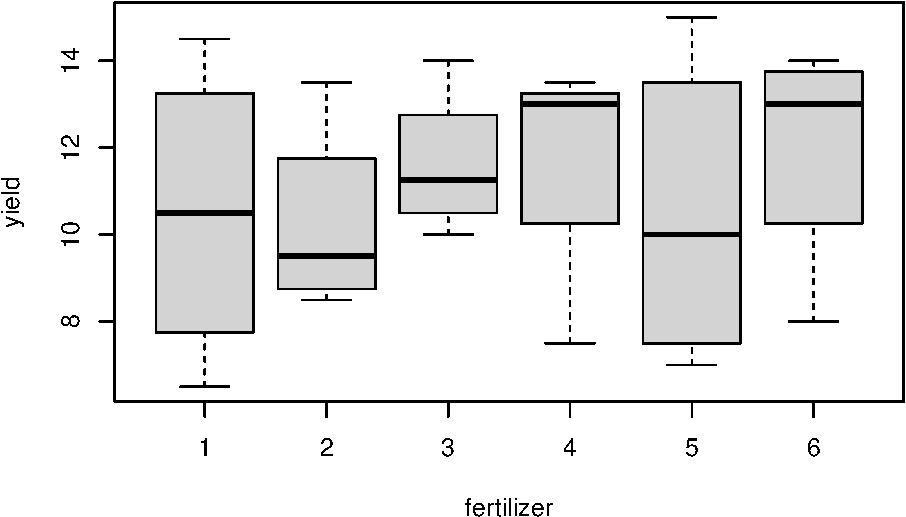
\includegraphics{bookdown_math3014-6027_files/figure-latex/ex2-eda-1} 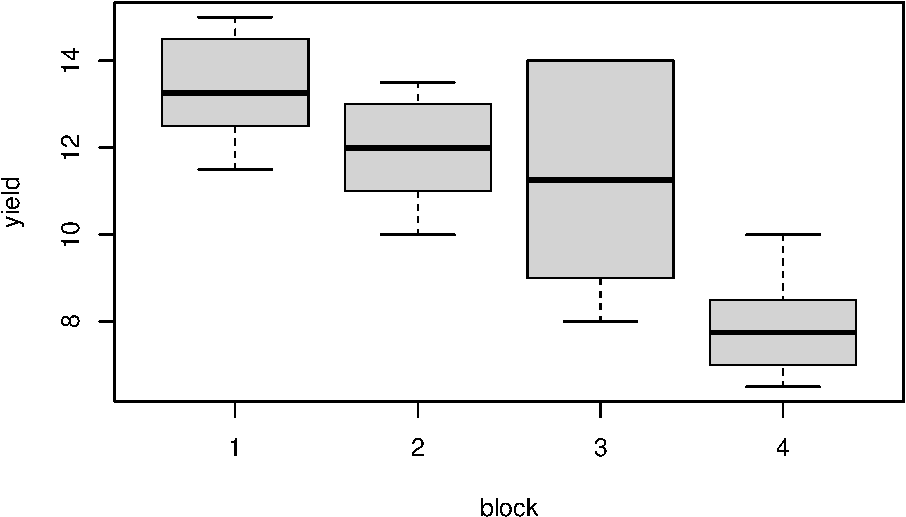
\includegraphics{bookdown_math3014-6027_files/figure-latex/ex2-eda-2} 

   }

   \caption{Blackcurrent experiment: yield against treatment and block.}\label{fig:ex2-eda}
   \end{figure}

  There are substantial differences in average responses between blocks; differences between treatment means are smaller. These plots are only meaningful because this design is an RCBD, and each treatment occurs in each block.

  The unit-block-treatment model is \emph{additive}; that is, we assume the effect of each treatment does not vary for each block. Therefore we also need to check that there are no substantive interactions between treatments and blocks. We will do this graphically.

\begin{Shaded}
\begin{Highlighting}[]
\FunctionTok{with}\NormalTok{(blackcurrent,}
  \FunctionTok{interaction.plot}\NormalTok{(fertilizer, block, yield, }\AttributeTok{xlab =} \StringTok{\textquotesingle{}Treatment\textquotesingle{}}\NormalTok{, }\AttributeTok{ylab =} \StringTok{\textquotesingle{}Yield\textquotesingle{}}\NormalTok{, }\AttributeTok{trace.label =} \StringTok{\textquotesingle{}Block\textquotesingle{}}\NormalTok{)}
\NormalTok{)}
\end{Highlighting}
\end{Shaded}

  \begin{figure}

   {\centering 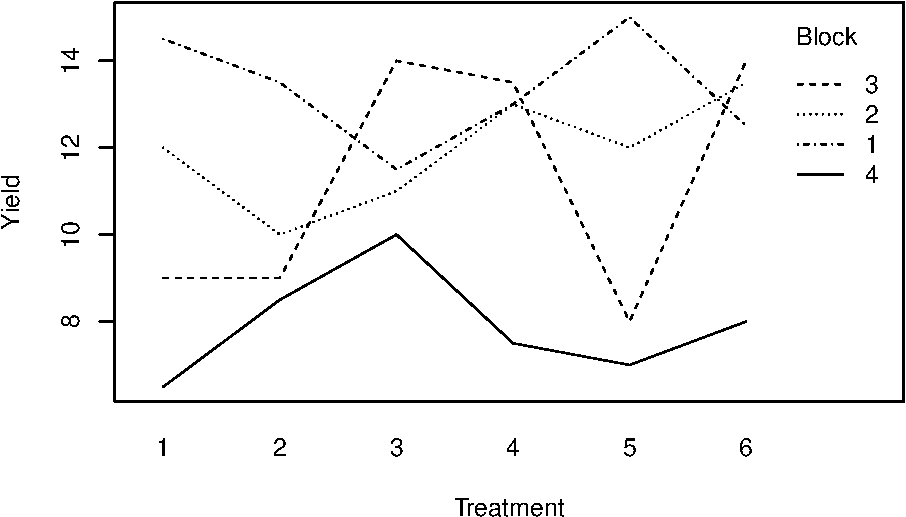
\includegraphics{bookdown_math3014-6027_files/figure-latex/ex2-interaction-1} 

   }

   \caption{Blackcurrent experiment: treatment-block interaction plot.}\label{fig:ex2-interaction}
   \end{figure}

  Figure \ref{fig:ex2-interaction} plots the treatment means within each block. While there are clear differences between blocks, the differences between treatments do not seem to vary systematically between blocks.
\item
  We now fit a linear model, and perform an F-test for the hypothesis \(H_0: \tau_1 = \tau_2 = \tau_3 = \tau_4 = \tau_5 = \tau_6 = 0\).

\begin{Shaded}
\begin{Highlighting}[]
\NormalTok{blackcurrent.lm }\OtherTok{\textless{}{-}} \FunctionTok{lm}\NormalTok{(yield }\SpecialCharTok{\textasciitilde{}}\NormalTok{ block }\SpecialCharTok{+}\NormalTok{ fertilizer, }\AttributeTok{data =}\NormalTok{ blackcurrent)}
\FunctionTok{anova}\NormalTok{(blackcurrent.lm)}
\end{Highlighting}
\end{Shaded}

\begin{verbatim}
## Analysis of Variance Table
## 
## Response: yield
##            Df Sum Sq Mean Sq F value Pr(>F)   
## block       3   94.9   31.62    8.90 0.0013 **
## fertilizer  5   11.8    2.36    0.66 0.6564   
## Residuals  15   53.3    3.55                  
## ---
## Signif. codes:  0 '***' 0.001 '**' 0.01 '*' 0.05 '.' 0.1 ' ' 1
\end{verbatim}

  The ``treatment'' row of the ANOVA table compares the model including blocks and treatments to that only containing blocks. This comparison tests the above null hypothesis. We can see here that there is no evidence to reject \(H_0\) (p-value = 0.6564). This outcome is not surprising, given the tabular and graphical summaries we saw above. The block sum of squares is large, but we do not perform formal hypothesis testing for blocks.

  Out of curiousity, we can also assess the ``efficiency'' of blocking by comparing the estimate of \(\sigma^2\) from the block design with the estimate that would result from ignoring the blocks, treating the experiment as a CRD and fitting a unit-treatment model.

\begin{Shaded}
\begin{Highlighting}[]
\NormalTok{blackcurrent\_crd.lm }\OtherTok{\textless{}{-}} \FunctionTok{lm}\NormalTok{(yield }\SpecialCharTok{\textasciitilde{}}\NormalTok{ fertilizer, }\AttributeTok{data =}\NormalTok{ blackcurrent)}
\FunctionTok{summary}\NormalTok{(blackcurrent\_crd.lm)}\SpecialCharTok{$}\NormalTok{sig}\SpecialCharTok{\^{}}\DecValTok{2} \SpecialCharTok{/} \FunctionTok{summary}\NormalTok{(blackcurrent.lm)}\SpecialCharTok{$}\NormalTok{sig}\SpecialCharTok{\^{}}\DecValTok{2}
\end{Highlighting}
\end{Shaded}

\begin{verbatim}
## [1] 2.316
\end{verbatim}

  The estimate of \(\sigma^2\) from the CRD is more the two times greater than the estimate from the block design, meaning about 100\% more observations would be needed in the CRD to get the same level of precision as the RCBD.
\item
  We now examine residual diagnostics, to check the assumptions of our model:

  \begin{itemize}
  \tightlist
  \item
    constant variance, with respect to the mean response, the treatment and the block
  \item
    normality of residuals
  \item
    additive treatment and block effects (already assessed in Fig \ref{fig:ex2-interaction}).
  \end{itemize}

\begin{Shaded}
\begin{Highlighting}[]
\NormalTok{standres }\OtherTok{\textless{}{-}} \FunctionTok{rstandard}\NormalTok{(blackcurrent.lm)}
\NormalTok{fitted }\OtherTok{\textless{}{-}} \FunctionTok{fitted}\NormalTok{(blackcurrent.lm)}
\FunctionTok{par}\NormalTok{(}\AttributeTok{mfrow =} \FunctionTok{c}\NormalTok{(}\DecValTok{1}\NormalTok{, }\DecValTok{3}\NormalTok{), }\AttributeTok{pty =} \StringTok{"s"}\NormalTok{)}
\FunctionTok{with}\NormalTok{(blackcurrent, \{}
  \FunctionTok{plot}\NormalTok{(fertilizer, standres, }\AttributeTok{xlab =} \StringTok{"Treatment"}\NormalTok{, }\AttributeTok{ylab =} \StringTok{"Standarised residuals"}\NormalTok{)}
  \FunctionTok{plot}\NormalTok{(block, standres, }\AttributeTok{xlab =} \StringTok{"Block"}\NormalTok{, }\AttributeTok{ylab =} \StringTok{"Standarised residuals"}\NormalTok{)}
  \FunctionTok{plot}\NormalTok{(fitted, standres, }\AttributeTok{xlab =} \StringTok{"Fitted value"}\NormalTok{, }\AttributeTok{ylab =} \StringTok{"Standarised residuals"}\NormalTok{)}
\NormalTok{\})}
\end{Highlighting}
\end{Shaded}

  \begin{figure}

   {\centering 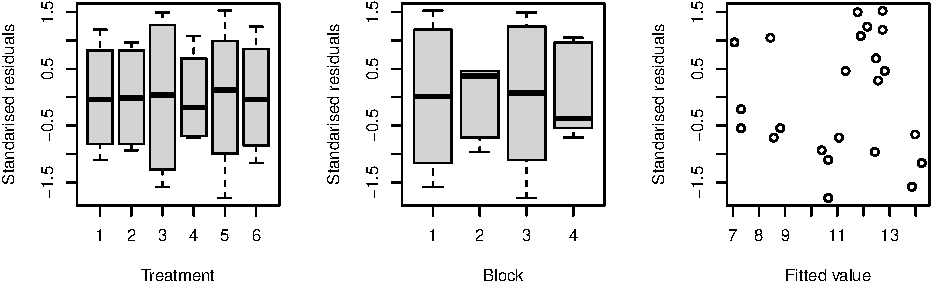
\includegraphics{bookdown_math3014-6027_files/figure-latex/ex2-residual-plots-1-1} 

   }

   \caption{Blackcurrent experiment: Residuals against treatments (left), blocks (middle) and fitted values (right).}\label{fig:ex2-residual-plots-1}
   \end{figure}

  The plots in Figure \ref{fig:ex2-residual-plots-1} do not show any serious evidence of non-constant variance (maybe very slightly for blocks), and no large outliers.

\begin{Shaded}
\begin{Highlighting}[]
 \FunctionTok{par}\NormalTok{(}\AttributeTok{pty =} \StringTok{"s"}\NormalTok{) }
 \FunctionTok{qqnorm}\NormalTok{(standres, }\AttributeTok{main =} \StringTok{""}\NormalTok{)}
\end{Highlighting}
\end{Shaded}

  \begin{figure}

   {\centering 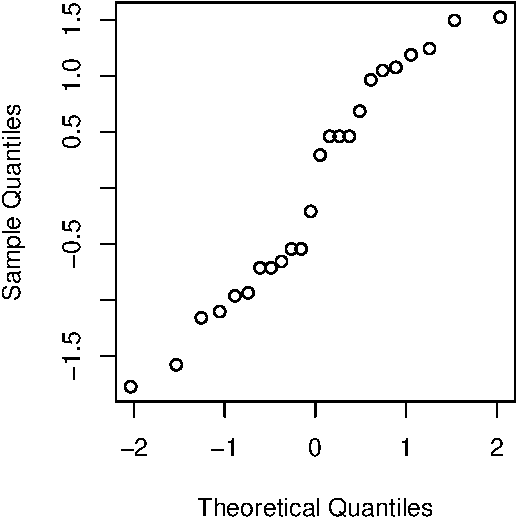
\includegraphics{bookdown_math3014-6027_files/figure-latex/ex2-residual-plots-2-1} 

   }

   \caption{Blackcurrent experiment: Normal probability plot for standardised residuals.}\label{fig:ex2-residual-plots-2}
   \end{figure}

  Figure \ref{fig:ex2-residual-plots-2} shows the residuals lie roughly on a straight line when plotted against theoretical normal quantiles, and hence the assumption of normally distributed errors seems reasonable.
\item
  There is no evidence of a difference between treatments, so we would not normally test each pairwise difference. However, if we did, we could use the following code.

\begin{Shaded}
\begin{Highlighting}[]
\NormalTok{blackcurrent.emm }\OtherTok{\textless{}{-}}\NormalTok{ emmeans}\SpecialCharTok{::}\FunctionTok{emmeans}\NormalTok{(blackcurrent.lm, }\SpecialCharTok{\textasciitilde{}}\NormalTok{ fertilizer)}
\FunctionTok{pairs}\NormalTok{(blackcurrent.emm)}
\end{Highlighting}
\end{Shaded}

\begin{verbatim}
##  contrast estimate   SE df t.ratio p.value
##  1 - 2       0.250 1.33 15   0.188  1.0000
##  1 - 3      -1.125 1.33 15  -0.844  0.9541
##  1 - 4      -1.250 1.33 15  -0.938  0.9303
##  1 - 5       0.000 1.33 15   0.000  1.0000
##  1 - 6      -1.500 1.33 15  -1.125  0.8635
##  2 - 3      -1.375 1.33 15  -1.031  0.9000
##  2 - 4      -1.500 1.33 15  -1.125  0.8635
##  2 - 5      -0.250 1.33 15  -0.188  1.0000
##  2 - 6      -1.750 1.33 15  -1.313  0.7741
##  3 - 4      -0.125 1.33 15  -0.094  1.0000
##  3 - 5       1.125 1.33 15   0.844  0.9541
##  3 - 6      -0.375 1.33 15  -0.281  0.9997
##  4 - 5       1.250 1.33 15   0.938  0.9303
##  4 - 6      -0.250 1.33 15  -0.188  1.0000
##  5 - 6      -1.500 1.33 15  -1.125  0.8635
## 
## Results are averaged over the levels of: block 
## P value adjustment: tukey method for comparing a family of 6 estimates
\end{verbatim}
\end{enumerate}

\begin{enumerate}
\def\labelenumi{\arabic{enumi}.}
\setcounter{enumi}{2}
\tightlist
\item
  Prove that \(2k/\lambda t > 2/b\), and use this result to compare the precision of a pairwise treatment comparison from a BIBD with block size \(k\) and an RCBD, both with \(t\) treatments in \(b\) blocks.
\end{enumerate}

Solution

From the notes, \(r = bk / t\) and hence \(k = rt / b\). Therefore

\begin{align*}
\frac{2k}{\lambda t} & = \frac{2rt}{\lambda b t} \\
& = \frac{2r}{\lambda b} \\
& = \frac{2}{b}\times\frac{r}{\lambda} \\
& > \frac{2}{b}\,,
\end{align*}

as \(r / \lambda > 1\). The variance of the estimator of a pairwise comparison is

\[
\mbox{var}_{\mbox{RCBD}}\left(\tau_i - \tau_j\right) = \frac{2\sigma^2}{b}\,,
\]

for a RCBD with \(b\) blocks, and

\[
\mbox{var}_{\mbox{BIBD}}\left(\tau_i - \tau_j\right) = \frac{2k\sigma^2}{\lambda t}\,,
\]

for a BIBD. Hence, we can see that the ratio of these variances is

\[
\frac{kb}{\lambda t} > 1\,,
\]

and hence the variance for a BIBD is larger, i.e.~incomplete blocks results in less precise treatment comparisons.

\begin{enumerate}
\def\labelenumi{\arabic{enumi}.}
\setcounter{enumi}{3}
\tightlist
\item
  Construct a BIBD for \(t=5\) treatments in \(b=5\) blocks of size \(k=4\) units. What are \(r\) and \(\lambda\) for your design? Compare your design to a RCBD via the efficiency for estimating a pairwise treatment difference.
\end{enumerate}

Solution

Here, \(b = {t \choose k} = {5 \choose 4} = 5\), and hence we can use the ``naive'' construction method from the notes, where we can form one block from each possible subset of \(k=4\) treatments. This design will have \(r = {4 \choose 3} = 4\) and \(\lambda = {3 \choose 2} = 3\).

\begin{Shaded}
\begin{Highlighting}[]
\NormalTok{bibd }\OtherTok{\textless{}{-}} \FunctionTok{t}\NormalTok{(}\FunctionTok{combn}\NormalTok{(}\DecValTok{1}\SpecialCharTok{:}\DecValTok{5}\NormalTok{, }\DecValTok{4}\NormalTok{))}
\FunctionTok{rownames}\NormalTok{(bibd) }\OtherTok{\textless{}{-}} \FunctionTok{paste}\NormalTok{(}\StringTok{"Block"}\NormalTok{, }\DecValTok{1}\SpecialCharTok{:}\DecValTok{5}\NormalTok{)}
\NormalTok{knitr}\SpecialCharTok{::}\FunctionTok{kable}\NormalTok{(bibd, }\AttributeTok{caption =} \StringTok{"BIBD for $t = 5$ treatments in $b=5$ blocks of size $k=4$."}\NormalTok{)}
\end{Highlighting}
\end{Shaded}

\begin{table}

\caption{\label{tab:naive-bibd-construction}BIBD for $t = 5$ treatments in $b=5$ blocks of size $k=4$.}
\centering
\begin{tabular}[t]{l|r|r|r|r}
\hline
Block 1 & 1 & 2 & 3 & 4\\
\hline
Block 2 & 1 & 2 & 3 & 5\\
\hline
Block 3 & 1 & 2 & 4 & 5\\
\hline
Block 4 & 1 & 3 & 4 & 5\\
\hline
Block 5 & 2 & 3 & 4 & 5\\
\hline
\end{tabular}
\end{table}

From Question 3, the efficiency of this BIBD compared to a RCBD with \(b=5\) blocks of size \(k=5\) is given by \(\frac{\lambda t}{kb} = 0.75\). So variances will be 25\% larger under the BIBD.

\begin{enumerate}
\def\labelenumi{\arabic{enumi}.}
\setcounter{enumi}{4}
\item
  Consider an experiment for testing the abrasion resistance of rubber-coated fabric. There are four types of material, denoted A - D. The response is the loss in weight in 0.1 milligrams (mg) over a standard period of time. The testing machine has four positions, so four samples of material can be tested at a time. Past experience suggests that there may be differences between these positions, and there may be differences between each application of the testing machine (due to changes in set-up). Therefore, we have two blocking variables, ``Position'' and ``Application''. For this experiment, we use a \textbf{latin square} design, as follows.

\begin{Shaded}
\begin{Highlighting}[]
\NormalTok{fabric }\OtherTok{\textless{}{-}} \FunctionTok{data.frame}\NormalTok{(}\AttributeTok{material =} \FunctionTok{factor}\NormalTok{(}\FunctionTok{c}\NormalTok{(}\StringTok{\textquotesingle{}C\textquotesingle{}}\NormalTok{, }\StringTok{\textquotesingle{}D\textquotesingle{}}\NormalTok{, }\StringTok{\textquotesingle{}B\textquotesingle{}}\NormalTok{, }\StringTok{\textquotesingle{}A\textquotesingle{}}\NormalTok{, }\StringTok{\textquotesingle{}A\textquotesingle{}}\NormalTok{, }\StringTok{\textquotesingle{}B\textquotesingle{}}\NormalTok{, }\StringTok{\textquotesingle{}D\textquotesingle{}}\NormalTok{, }\StringTok{\textquotesingle{}C\textquotesingle{}}\NormalTok{, }
                           \StringTok{\textquotesingle{}D\textquotesingle{}}\NormalTok{, }\StringTok{\textquotesingle{}C\textquotesingle{}}\NormalTok{, }\StringTok{\textquotesingle{}A\textquotesingle{}}\NormalTok{, }\StringTok{\textquotesingle{}B\textquotesingle{}}\NormalTok{, }\StringTok{\textquotesingle{}B\textquotesingle{}}\NormalTok{, }\StringTok{\textquotesingle{}A\textquotesingle{}}\NormalTok{, }\StringTok{\textquotesingle{}C\textquotesingle{}}\NormalTok{, }\StringTok{\textquotesingle{}D\textquotesingle{}}\NormalTok{)),}
               \AttributeTok{position =} \FunctionTok{rep}\NormalTok{(}\FunctionTok{factor}\NormalTok{(}\DecValTok{1}\SpecialCharTok{:}\DecValTok{4}\NormalTok{), }\DecValTok{4}\NormalTok{),}
               \AttributeTok{application =} \FunctionTok{rep}\NormalTok{(}\FunctionTok{factor}\NormalTok{(}\DecValTok{1}\SpecialCharTok{:}\DecValTok{4}\NormalTok{), }\FunctionTok{rep}\NormalTok{(}\DecValTok{4}\NormalTok{, }\DecValTok{4}\NormalTok{)),}
               \AttributeTok{weight =} \FunctionTok{c}\NormalTok{(}\DecValTok{235}\NormalTok{, }\DecValTok{236}\NormalTok{, }\DecValTok{218}\NormalTok{, }\DecValTok{268}\NormalTok{,}
                            \DecValTok{251}\NormalTok{, }\DecValTok{241}\NormalTok{, }\DecValTok{227}\NormalTok{, }\DecValTok{229}\NormalTok{, }
                            \DecValTok{234}\NormalTok{, }\DecValTok{273}\NormalTok{, }\DecValTok{274}\NormalTok{, }\DecValTok{226}\NormalTok{,}
                            \DecValTok{195}\NormalTok{, }\DecValTok{270}\NormalTok{, }\DecValTok{230}\NormalTok{, }\DecValTok{225}\NormalTok{)}
\NormalTok{                 )}
\NormalTok{knitr}\SpecialCharTok{::}\FunctionTok{kable}\NormalTok{(}
\NormalTok{ tidyr}\SpecialCharTok{::}\FunctionTok{pivot\_wider}\NormalTok{(fabric, }\AttributeTok{id\_cols =}\NormalTok{ application, }\AttributeTok{names\_from =}\NormalTok{ position, }
                \AttributeTok{values\_from =}\NormalTok{ material),}
 \AttributeTok{col.names =} \FunctionTok{c}\NormalTok{(}\StringTok{"Application"}\NormalTok{, }\FunctionTok{paste}\NormalTok{(}\StringTok{"Position"}\NormalTok{, }\DecValTok{1}\SpecialCharTok{:}\DecValTok{4}\NormalTok{)))}
\end{Highlighting}
\end{Shaded}

  \begin{tabular}{l|l|l|l|l}
   \hline
   Application & Position 1 & Position 2 & Position 3 & Position 4\\
   \hline
   1 & C & D & B & A\\
   \hline
   2 & A & B & D & C\\
   \hline
   3 & D & C & A & B\\
   \hline
   4 & B & A & C & D\\
   \hline
   \end{tabular}

  The blocking variables are represented as the rows and columns of the square; the latin letters represent the different treatments. A latin square of order \(k\) is a \(k\times k\) square of \(k\) latin letters arranged so that each letter appears exactly once in each row and column (Sudoko squares are also examples of latin squares). To perform the experiment, the levels of the blocking factors are randomly assigned to the rows and the columns, and the different treatments to the letters. A latin square design is a special case of the more general class of \textbf{row column} designs for two blocking factors.

  A suitable unit-block-treatment model for a latin square design has the form

  \[
   y_{ijk} = \mu + \beta_i + \gamma_j + \tau_k + \varepsilon_{ijk}\,,\qquad i,j,k = 1,\ldots, t\,,
   \]

  with \(\mu\) a constant parameter, \(\beta_i\) row block effects, \(\gamma_j\) column block effects and \(\tau_k\) the treatment effects. As usual, \(\varepsilon_{ijk}\sim N(0, \sigma^2)\), with errors from different units assumed independent. Note that not all combinations of \(i,j,k\) actually occur in the design; at the intersection of the \(i\)th row and \(j\)th column, only one of the \(t\) treatments is applied.

  \begin{enumerate}
  \def\labelenumii{\alph{enumii}.}
  \item
    Write down a set of normal equations for the model parameters.
  \item
    It can be shown that the reduced normal equations for the treatment parameters \(\tau_1,\ldots, \tau_t\) have the form
    \[
     \hat{\tau}_k - \hat{\tau}_w = \bar{y}_{..j} - \bar{y}_{...}\,,
     \]
    with \(\hat{\tau}_w = \frac{1}{t}\sum_{k=1}^t\hat{\tau}_k\), \(\bar{y}_{..k} = \frac{1}{t}\sum_{i=1}^t\sum_{j=1}^tn_{ijk}y_{ijk}\) (mean for treatment \(k\)) and \(\bar{y}_{...} = \frac{1}{n}\sum_{i=1}^t\sum_{j=1}^t\sum_{k=1}^tn_{ij}y_{ijk}\) (overall mean) where \(n_{ijk} = 1\) if treatment \(k\) occurs at the intersection of row \(i\) and column \(j\) and zero otherwise, and \(\sum_{i=1}^t\sum_{j=1}^tn_{ijk} = t\) for all \(k=1, \ldots, t\).

    Demonstrate that any contrast can therefore be estimated from this design, and derive the variance of the estimator of \(\sum_{k=1}^tc_k\tau_k\).
  \end{enumerate}

  The data for this experiment is as follows, where the entries in the table give the response for the corresponding treatment:

\begin{Shaded}
\begin{Highlighting}[]
\NormalTok{knitr}\SpecialCharTok{::}\FunctionTok{kable}\NormalTok{(}
\NormalTok{ tidyr}\SpecialCharTok{::}\FunctionTok{pivot\_wider}\NormalTok{(fabric, }\AttributeTok{id\_cols =}\NormalTok{ application, }\AttributeTok{names\_from =}\NormalTok{ position, }
                \AttributeTok{values\_from =}\NormalTok{ weight),}
 \AttributeTok{col.names =} \FunctionTok{c}\NormalTok{(}\StringTok{"Application"}\NormalTok{, }\FunctionTok{paste}\NormalTok{(}\StringTok{"Position"}\NormalTok{, }\DecValTok{1}\SpecialCharTok{:}\DecValTok{4}\NormalTok{)))}
\end{Highlighting}
\end{Shaded}

  \begin{tabular}{l|r|r|r|r}
   \hline
   Application & Position 1 & Position 2 & Position 3 & Position 4\\
   \hline
   1 & 235 & 236 & 218 & 268\\
   \hline
   2 & 251 & 241 & 227 & 229\\
   \hline
   3 & 234 & 273 & 274 & 226\\
   \hline
   4 & 195 & 270 & 230 & 225\\
   \hline
   \end{tabular}

  \begin{enumerate}
  \def\labelenumii{\alph{enumii}.}
  \setcounter{enumii}{2}
  \tightlist
  \item
    For this data, test if there is a significant difference between materials. If there is, conduct multiple comparisons of all pairs at an experimentwise type I error rate of 5\%.
  \end{enumerate}
\end{enumerate}

Solution

\begin{enumerate}
\def\labelenumi{\alph{enumi}.}
\item
  We start by writing the model in matrix form:

  \begin{align*}
   \boldsymbol{y}& = \boldsymbol{1}_n\mu + X_1\boldsymbol{\beta} + X_2\boldsymbol{\gamma} + X_3\boldsymbol{\tau} + \boldsymbol{\varepsilon}\\
   & = W\boldsymbol{\alpha} + \boldsymbol{\varepsilon}\,, 
   \end{align*}

  with \(W = (\boldsymbol{1}_n, X_1, X_2, X_3)\), \(X_1\), \(X_2\) and \(X_3\) being \(n \times t\) model matrices for row blocks, column blocks and treatments, respectively, \(\boldsymbol{\alpha}^{\mathrm{T}} = (\mu, \boldsymbol{\beta}^{\mathrm{T}}, \boldsymbol{\gamma}^{\mathrm{T}}, \boldsymbol{\tau}^{\mathrm{T}})\) being a \((1+3t)\)-vector of parameters, and \(\boldsymbol{\varepsilon}\sim N(\boldsymbol{0}_n, I_n\sigma^2)\).

  The normal equations are given by \(W^{\mathrm{T}}W\hat{\boldsymbol{\alpha}} = W^{\mathrm{T}}\boldsymbol{y}\), which can be expanded out to give the following four matrix equations:

  \begin{align}
  n\hat{\mu} + \boldsymbol{1}_n^{\mathrm{T}}X_1\hat{\boldsymbol{\beta}} + \boldsymbol{1}_n^{\mathrm{T}}X_2\hat{\boldsymbol{\gamma}} + \boldsymbol{1}_n^{\mathrm{T}}X_3\hat{\boldsymbol{\tau}} & = \boldsymbol{1}_n^{\mathrm{T}}\boldsymbol{y}\,, \label{eq:rc-normal-1}\\
  X_1^{\mathrm{T}}\boldsymbol{1}_n\hat{\mu} + X_1^{\mathrm{T}}X_1\hat{\boldsymbol{\beta}} + X_1^{\mathrm{T}}X_2\hat{\boldsymbol{\gamma}} + X_1^{\mathrm{T}}X_3\hat{\boldsymbol{\tau}} & = X_1^{\mathrm{T}}\boldsymbol{y}\,, \label{eq:rc-normal-2}\\
  X_2^{\mathrm{T}}\boldsymbol{1}_n\hat{\mu} + X_2^{\mathrm{T}}X_1\hat{\boldsymbol{\beta}} + X_2^{\mathrm{T}}X_2\hat{\boldsymbol{\gamma}} + X_2^{\mathrm{T}}X_3\hat{\boldsymbol{\tau}} & = X_2^{\mathrm{T}}\boldsymbol{y}\,, \label{eq:rc-normal-3}\\
  X_3^{\mathrm{T}}\boldsymbol{1}_n\hat{\mu} + X_3^{\mathrm{T}}X_1\hat{\boldsymbol{\beta}} + X_3^{\mathrm{T}}X_2\hat{\boldsymbol{\gamma}} + X_3^{\mathrm{T}}X_3\hat{\boldsymbol{\tau}} & = X_3^{\mathrm{T}}\boldsymbol{y}\,. \label{eq:rc-normal-4}\\
   \end{align}
\item
  From the reduced normal equations given in the question, we have

  \begin{align*}
   \sum_{k=1}^tc_k\left(\hat{\tau}_k - \hat{\tau}_w\right) & = \sum_{k=1}^tc_k\hat{\tau}_k \\
   & = \sum_{k=1}^tc_k\left(\bar{y}_{..k} - \bar{y}_{...}\right) \\
   & = \sum_{k=1}^tc_k\bar{y}_{..k}\,,
   \end{align*}

  as \(\sum_{k=1}^tc_k\hat{\tau}_w = \sum_{k=1}^tc_k\bar{y}_{...} = 0\), as neither \(\hat{\tau}_w\) or \(\bar{y}_{...}\) depend on \(k\). Hence,

  \[
   \widehat{\boldsymbol{c}^{\mathrm{T}}\boldsymbol{\tau}} = \sum_{k=1}^tc_k\bar{y}_{..k}\,.
   \]

  Or notice that the reduced normal equations for this design are the same as for a CRD with each treatment replicated \(t\) times.
\item
  We conduct these hypothesis tests using \texttt{R}.

\begin{Shaded}
\begin{Highlighting}[]
\NormalTok{fabric.lm }\OtherTok{\textless{}{-}} \FunctionTok{lm}\NormalTok{(weight }\SpecialCharTok{\textasciitilde{}}\NormalTok{ position }\SpecialCharTok{+}\NormalTok{ application }\SpecialCharTok{+}\NormalTok{ material, }\AttributeTok{data =}\NormalTok{ fabric)}
\FunctionTok{anova}\NormalTok{(fabric.lm)}
\end{Highlighting}
\end{Shaded}

\begin{verbatim}
## Analysis of Variance Table
## 
## Response: weight
##             Df Sum Sq Mean Sq F value  Pr(>F)    
## position     3   1468     489    7.99 0.01617 *  
## application  3    986     329    5.37 0.03901 *  
## material     3   4621    1540   25.15 0.00085 ***
## Residuals    6    368      61                    
## ---
## Signif. codes:  0 '***' 0.001 '**' 0.01 '*' 0.05 '.' 0.1 ' ' 1
\end{verbatim}

  The ``material'' line of the ANOVA table compares the models with and without the effects for material (but both models including the blocking factors). There is clearly a significant effect of material.

\begin{Shaded}
\begin{Highlighting}[]
\NormalTok{fabric.emm }\OtherTok{\textless{}{-}}\NormalTok{ emmeans}\SpecialCharTok{::}\FunctionTok{emmeans}\NormalTok{(fabric.lm, }\SpecialCharTok{\textasciitilde{}}\NormalTok{ material)}
\NormalTok{fabric.pairs }\OtherTok{\textless{}{-}} \FunctionTok{transform}\NormalTok{(}\FunctionTok{pairs}\NormalTok{(fabric.emm))}
\NormalTok{dplyr}\SpecialCharTok{::}\FunctionTok{mutate}\NormalTok{(fabric.pairs, }\AttributeTok{reject =}\NormalTok{ p.value }\SpecialCharTok{\textless{}} \FloatTok{0.05}\NormalTok{)}
\end{Highlighting}
\end{Shaded}

\begin{verbatim}
##   contrast estimate    SE df t.ratio  p.value reject
## 1    A - B    45.75 5.534  6   8.267 0.000703   TRUE
## 2    A - C    24.00 5.534  6   4.337 0.019036   TRUE
## 3    A - D    35.25 5.534  6   6.370 0.002866   TRUE
## 4    B - C   -21.75 5.534  6  -3.930 0.029477   TRUE
## 5    B - D   -10.50 5.534  6  -1.897 0.320631  FALSE
## 6    C - D    11.25 5.534  6   2.033 0.274277  FALSE
\end{verbatim}
\end{enumerate}

Using an experiment-wise error rate of 5\%, we see significant differences between materials A and B, A and C, A and D, and B and C.

\hypertarget{factorial}{%
\chapter{Factorial experiments}\label{factorial}}

In Chapters \ref{crd} and \ref{blocking}, we assumed the objective of the experiment was to investigate \(t\) \textbf{unstructured} treatments, defined only as a collection of distinct entities (drugs, advertisements, receipes, etc.). That is, there was not necessarily any explicit relationship between the treatments (although we could clearly choose which paticular comparisons between treatments were of interest via choice of contrast).

In many experiments, particularly in industry, engineering and the physical sciences, the treatments are actually defined via the choice of a \textbf{level} relating to each of a set of \textbf{factors}. We will focus on the commonly occurring case of factors at \textbf{two levels}. For example, consider the below experiment from the pharmaceutical industry.

\begin{example}
\protect\hypertarget{exm:factorial-desilylation}{}\label{exm:factorial-desilylation}

Desilylation experiment \citep{Owen2001}

In this experiment, performed at GlaxoSmithKline, the aim was to optimise the desilylation\footnote{Desilylation is a process of removing silyl, SiH\(_3\) a silicon hydride, from a compound.} of an ether into an alcohol, which was a key step in the synthesis of a particular antibiotic. There were \(t=16\) treatments, defined via the settings of four different factors, as given in Table \ref{tab:factorial-desilylation-data}.

\begin{Shaded}
\begin{Highlighting}[]
\NormalTok{desilylation }\OtherTok{\textless{}{-}}\NormalTok{ FrF2}\SpecialCharTok{::}\FunctionTok{FrF2}\NormalTok{(}\AttributeTok{nruns =} \DecValTok{16}\NormalTok{, }\AttributeTok{nfactors =} \DecValTok{4}\NormalTok{, }\AttributeTok{randomize =}\NormalTok{ F,}
                           \AttributeTok{factor.names =} \FunctionTok{list}\NormalTok{(}\AttributeTok{temp =} \FunctionTok{c}\NormalTok{(}\DecValTok{10}\NormalTok{, }\DecValTok{20}\NormalTok{), }\AttributeTok{time =} \FunctionTok{c}\NormalTok{(}\DecValTok{19}\NormalTok{, }\DecValTok{25}\NormalTok{),}
                                               \AttributeTok{solvent =} \FunctionTok{c}\NormalTok{(}\DecValTok{5}\NormalTok{, }\DecValTok{7}\NormalTok{), }\AttributeTok{reagent =} \FunctionTok{c}\NormalTok{(}\DecValTok{1}\NormalTok{, }\FloatTok{1.33}\NormalTok{)))}
\NormalTok{yield }\OtherTok{\textless{}{-}} \FunctionTok{c}\NormalTok{(}\FloatTok{82.93}\NormalTok{, }\FloatTok{94.04}\NormalTok{, }\FloatTok{88.07}\NormalTok{, }\FloatTok{93.97}\NormalTok{, }\FloatTok{77.21}\NormalTok{, }\FloatTok{92.99}\NormalTok{, }\FloatTok{83.60}\NormalTok{, }\FloatTok{94.38}\NormalTok{, }
           \FloatTok{88.68}\NormalTok{, }\FloatTok{94.30}\NormalTok{, }\FloatTok{93.00}\NormalTok{, }\FloatTok{93.42}\NormalTok{, }\FloatTok{84.86}\NormalTok{, }\FloatTok{94.26}\NormalTok{, }\FloatTok{88.71}\NormalTok{, }\FloatTok{94.66}\NormalTok{)}
\NormalTok{desilylation }\OtherTok{\textless{}{-}} \FunctionTok{data.frame}\NormalTok{(desilylation, }\AttributeTok{yield =}\NormalTok{ yield)}
\FunctionTok{rownames}\NormalTok{(desilylation) }\OtherTok{\textless{}{-}} \FunctionTok{paste}\NormalTok{(}\StringTok{"Trt"}\NormalTok{, }\DecValTok{1}\SpecialCharTok{:}\DecValTok{16}\NormalTok{)}
\NormalTok{knitr}\SpecialCharTok{::}\FunctionTok{kable}\NormalTok{(desilylation, }
             \AttributeTok{col.names =} \FunctionTok{c}\NormalTok{(}\StringTok{"Temp (degrees C)"}\NormalTok{, }\StringTok{"Time (hours)"}\NormalTok{, }\StringTok{"Solvent (vol.)"}\NormalTok{, }
                           \StringTok{"Reagent (equiv.)"}\NormalTok{, }\StringTok{"Yield (\%)"}\NormalTok{),}
             \AttributeTok{caption =} \StringTok{"Desilylation experiment: 16 treatments defined }
\StringTok{             by settings of four factors, with response (yield)."}\NormalTok{)}
\end{Highlighting}
\end{Shaded}

\begin{table}

\caption{\label{tab:factorial-desilylation-data}Desilylation experiment: 16 treatments defined 
             by settings of four factors, with response (yield).}
\centering
\begin{tabular}[t]{l|l|l|l|l|r}
\hline
  & Temp (degrees C) & Time (hours) & Solvent (vol.) & Reagent (equiv.) & Yield (\%)\\
\hline
Trt 1 & 10 & 19 & 5 & 1 & 82.93\\
\hline
Trt 2 & 20 & 19 & 5 & 1 & 94.04\\
\hline
Trt 3 & 10 & 25 & 5 & 1 & 88.07\\
\hline
Trt 4 & 20 & 25 & 5 & 1 & 93.97\\
\hline
Trt 5 & 10 & 19 & 7 & 1 & 77.21\\
\hline
Trt 6 & 20 & 19 & 7 & 1 & 92.99\\
\hline
Trt 7 & 10 & 25 & 7 & 1 & 83.60\\
\hline
Trt 8 & 20 & 25 & 7 & 1 & 94.38\\
\hline
Trt 9 & 10 & 19 & 5 & 1.33 & 88.68\\
\hline
Trt 10 & 20 & 19 & 5 & 1.33 & 94.30\\
\hline
Trt 11 & 10 & 25 & 5 & 1.33 & 93.00\\
\hline
Trt 12 & 20 & 25 & 5 & 1.33 & 93.42\\
\hline
Trt 13 & 10 & 19 & 7 & 1.33 & 84.86\\
\hline
Trt 14 & 20 & 19 & 7 & 1.33 & 94.26\\
\hline
Trt 15 & 10 & 25 & 7 & 1.33 & 88.71\\
\hline
Trt 16 & 20 & 25 & 7 & 1.33 & 94.66\\
\hline
\end{tabular}
\end{table}

Each treatment is defined by the choice of one of two levels for each of the four factors. In the \texttt{R} code above, we have used the function \texttt{FrF2} (from the package of the same name) to generate all \(t = 2^4 = 16\) combinations of the two levels of these four factors. We come back to this function later in the chapter.

\end{example}

This \textbf{factorial treatment structure} lends itself to certain treatment contrasts being of natural interest.

\hypertarget{factorial-contrasts}{%
\section{Factorial contrasts}\label{factorial-contrasts}}

Throughout this chapter, we will assume there are no blocks or other restrictions on randomisation, and so we will assume a completely randomised design can be used. We start by assuming the same unit-treatment model as Chapter \ref{crd}:

\begin{equation}
y_{ij} = \mu + \tau_i + \varepsilon_{ij}\,, \quad i = 1, \ldots, t; j = 1, \ldots, n_i\,, \label{eq:factorial-utm}
\end{equation}

where \(y_{ij}\) is the response from the \(j\)th application of treatment \(i\), \(\mu\) is a constant parameter, \(\tau_i\) is the effect of the \(i\)th treatment, and \(\varepsilon_{ij}\) is the random individual effect from each experimental unit with \(\varepsilon_{ij} \sim N(0, \sigma^2)\) independent of other errors.

Now, the number of treatments \(t = 2^f\), where \(f\) equals the number of factors in the experiment.

For Example \ref{exm:factorial-desilylation}, we have \(t = 2^4 = 16\) and \(n_i = 1\) for all \(i=1,\ldots, 16\); that is, each of the 16 treatments are replicated once. In general, we shall assume common treatment replication \(n_i = r \ge 1\).

If we fit model \eqref{eq:factorial-utm} and compute the ANOVA table, we notice a particular issue with this design.

\begin{Shaded}
\begin{Highlighting}[]
\NormalTok{desilylation }\OtherTok{\textless{}{-}} \FunctionTok{data.frame}\NormalTok{(desilylation, }\AttributeTok{trt =} \FunctionTok{factor}\NormalTok{(}\DecValTok{1}\SpecialCharTok{:}\DecValTok{16}\NormalTok{))}
\NormalTok{desilylation.lm }\OtherTok{\textless{}{-}} \FunctionTok{lm}\NormalTok{(yield }\SpecialCharTok{\textasciitilde{}}\NormalTok{ trt, }\AttributeTok{data =}\NormalTok{ desilylation)}
\FunctionTok{anova}\NormalTok{(desilylation.lm)}
\end{Highlighting}
\end{Shaded}

\begin{verbatim}
## Analysis of Variance Table
## 
## Response: yield
##           Df Sum Sq Mean Sq F value Pr(>F)
## trt       15    427    28.5     NaN    NaN
## Residuals  0      0     NaN
\end{verbatim}

All available degrees of freedom are being used to estimate parameters in the mean (\(\mu\) and the treatment effects \(\tau_i\)). There are no degrees of freedom left to estimate \(\sigma^2\). This is due to a lack of treatment replication. Without replication in the design, model \eqref{eq:factorial-utm} is \textbf{saturated}, with as many treatments as there are observations and an unbiased estimate of \(\sigma^2\) cannot be obtained. We will return to this issue later.

\hypertarget{main-effects}{%
\subsection{Main effects}\label{main-effects}}

Studying Table \ref{tab:factorial-desilylation-data}, there are some comparisons between treatments which are obviously of interest. For example, comparing the average effect from the first 8 treatments with the average effect of the second 8, using

\[
\boldsymbol{c}^{\mathrm{T}}\boldsymbol{\tau} = \sum_{i=1}^tc_i\tau_i\,,
\]
with

\[
\boldsymbol{c}^{\mathrm{T}} = (-\boldsymbol{1}_8^{\mathrm{T}}, \boldsymbol{1}_8^{\mathrm{T}}) / 8\,.
\]

\begin{Shaded}
\begin{Highlighting}[]
\NormalTok{desilylation.emm }\OtherTok{\textless{}{-}}\NormalTok{ emmeans}\SpecialCharTok{::}\FunctionTok{emmeans}\NormalTok{(desilylation.lm, }\SpecialCharTok{\textasciitilde{}}\NormalTok{ trt)}
\NormalTok{reagent\_me.emmc }\OtherTok{\textless{}{-}} \ControlFlowTok{function}\NormalTok{(levs) }\FunctionTok{data.frame}\NormalTok{(}\StringTok{\textquotesingle{}reagent m.e.\textquotesingle{}} \OtherTok{=} \FunctionTok{rep}\NormalTok{(}\FunctionTok{c}\NormalTok{(}\SpecialCharTok{{-}}\DecValTok{1}\NormalTok{, }\DecValTok{1}\NormalTok{), }\FunctionTok{rep}\NormalTok{(}\DecValTok{8}\NormalTok{, }\DecValTok{2}\NormalTok{)) }\SpecialCharTok{/} \DecValTok{8}\NormalTok{)}
\NormalTok{emmeans}\SpecialCharTok{::}\FunctionTok{contrast}\NormalTok{(desilylation.emm, }\StringTok{\textquotesingle{}reagent\_me\textquotesingle{}}\NormalTok{)}
\end{Highlighting}
\end{Shaded}

\begin{verbatim}
##  contrast     estimate  SE df t.ratio p.value
##  reagent.m.e.     3.09 NaN  0     NaN     NaN
\end{verbatim}

This contrast compares the average treatment effect from the 8 treatments which have \texttt{reagent} set to its low level (1 equiv.) to the average effect from the 8 treatments which have \texttt{reagent} set to its high level. This is a ``fair'' comparison, as both of these sets of treatments have each of the combinations of the factors \texttt{temp}, \texttt{time} and \texttt{solvent} occuring equally often (twice here). Hence, the \textbf{main effect} of \texttt{reagent} is averaged over the levels of the other three factors.

As in Chapter \ref{crd}, we can estimate this treatment contrast by applying the same contrast coefficients to the treatment means,

\[
\widehat{\boldsymbol{c}^{\mathrm{T}}\boldsymbol{\tau}} = \sum_{i=1}^tc_i\bar{y}_{i.}\,,
\]
where, for this experiment, each \(\bar{y}_{i.}\) is the mean of a single observation (as there is no treatment replication). We see that inference about this contrast is not possible, as no standard error can be obtained.

\begin{definition}
\protect\hypertarget{def:main-effect}{}\label{def:main-effect}

The \textbf{main effect} of a factor \(A\) is defined as the difference in the average response from the high and low levels of the factor

\[
\mbox{ME}(A) = \bar{y}(A+) - \bar{y}(A-)\,,
\]
where \(\bar{y}(A+)\) is the average response when factor \(A\) is set to its high level, averaged across all combinations of levels of the other factors (with \(\bar{y}(A+)\) defined similarly for the low level of \(A\)).

\end{definition}

As we have averaged the response across the levels of the other factors, the intepretation of the main effect extends beyond this experiment. That is, we can use it to infer something about the system under study. Assuming model \eqref{eq:factorial-utm} is correct, any variation in the main effect can only come from random error in the observations. In fact,

\begin{align*}
\mbox{var}\{ME(A)\} & = \frac{\sigma^2}{n/2} + \frac{\sigma^2}{n/2} \\
& = \frac{4\sigma^2}{n}\,,
\end{align*}

and assuming \(r>1\),

\begin{equation}
\hat{\sigma}^2 = \frac{1}{2^f(r-1)} \sum_{i=1}^{2^f}\sum_{j=1}^r(y_{ij} - \bar{y}_{i.})^2\,,
\label{eq:factorial-sigma-hat-2}
\end{equation}

which is the residual mean square.

For Example \ref{exm:factorial-desilylation}, we can also calculate main effect estimates for the other three factors by defining appropriate contrasts in the treatments.

\begin{Shaded}
\begin{Highlighting}[]
\NormalTok{contrast.mat }\OtherTok{\textless{}{-}}\NormalTok{ FrF2}\SpecialCharTok{::}\FunctionTok{FrF2}\NormalTok{(}\AttributeTok{nruns =} \DecValTok{16}\NormalTok{, }\AttributeTok{nfactors =} \DecValTok{4}\NormalTok{, }\AttributeTok{randomize =}\NormalTok{ F, }
                           \AttributeTok{factor.names =} \FunctionTok{c}\NormalTok{(}\StringTok{"temp"}\NormalTok{, }\StringTok{"time"}\NormalTok{, }\StringTok{"solvent"}\NormalTok{, }\StringTok{"reagent"}\NormalTok{))}
\NormalTok{fac.contrasts.emmc }\OtherTok{\textless{}{-}} \ControlFlowTok{function}\NormalTok{(levs) }
\NormalTok{  dplyr}\SpecialCharTok{::}\FunctionTok{mutate\_all}\NormalTok{(}\FunctionTok{data.frame}\NormalTok{(contrast.mat), }\ControlFlowTok{function}\NormalTok{(x) }\FunctionTok{scale}\NormalTok{(}\FunctionTok{as.numeric}\NormalTok{(}\FunctionTok{as.character}\NormalTok{(x)), }\AttributeTok{scale =} \DecValTok{8}\NormalTok{))}
\NormalTok{main\_effect\_contrasts }\OtherTok{\textless{}{-}} \FunctionTok{fac.contrasts.emmc}\NormalTok{()}
\FunctionTok{rownames}\NormalTok{(main\_effect\_contrasts) }\OtherTok{\textless{}{-}} \FunctionTok{paste}\NormalTok{(}\StringTok{"Trt"}\NormalTok{, }\DecValTok{1}\SpecialCharTok{:}\DecValTok{16}\NormalTok{)}
\NormalTok{knitr}\SpecialCharTok{::}\FunctionTok{kable}\NormalTok{(main\_effect\_contrasts, }\AttributeTok{caption =} \StringTok{\textquotesingle{}Desilylation experiment: main effect contrast coefficients\textquotesingle{}}\NormalTok{, }\AttributeTok{col.names =} \FunctionTok{c}\NormalTok{(}\StringTok{"Temperature"}\NormalTok{, }\StringTok{"Time"}\NormalTok{, }\StringTok{"Solvent"}\NormalTok{, }\StringTok{"Reagent"}\NormalTok{))}
\end{Highlighting}
\end{Shaded}

\begin{table}

\caption{\label{tab:desilylation-all-me-contrasts}Desilylation experiment: main effect contrast coefficients}
\centering
\begin{tabular}[t]{l|r|r|r|r}
\hline
  & Temperature & Time & Solvent & Reagent\\
\hline
Trt 1 & -0.125 & -0.125 & -0.125 & -0.125\\
\hline
Trt 2 & 0.125 & -0.125 & -0.125 & -0.125\\
\hline
Trt 3 & -0.125 & 0.125 & -0.125 & -0.125\\
\hline
Trt 4 & 0.125 & 0.125 & -0.125 & -0.125\\
\hline
Trt 5 & -0.125 & -0.125 & 0.125 & -0.125\\
\hline
Trt 6 & 0.125 & -0.125 & 0.125 & -0.125\\
\hline
Trt 7 & -0.125 & 0.125 & 0.125 & -0.125\\
\hline
Trt 8 & 0.125 & 0.125 & 0.125 & -0.125\\
\hline
Trt 9 & -0.125 & -0.125 & -0.125 & 0.125\\
\hline
Trt 10 & 0.125 & -0.125 & -0.125 & 0.125\\
\hline
Trt 11 & -0.125 & 0.125 & -0.125 & 0.125\\
\hline
Trt 12 & 0.125 & 0.125 & -0.125 & 0.125\\
\hline
Trt 13 & -0.125 & -0.125 & 0.125 & 0.125\\
\hline
Trt 14 & 0.125 & -0.125 & 0.125 & 0.125\\
\hline
Trt 15 & -0.125 & 0.125 & 0.125 & 0.125\\
\hline
Trt 16 & 0.125 & 0.125 & 0.125 & 0.125\\
\hline
\end{tabular}
\end{table}

Estimates can be obtained by applying these coefficients to the observed treatment means.

\begin{Shaded}
\begin{Highlighting}[]
\FunctionTok{t}\NormalTok{(}\FunctionTok{as.matrix}\NormalTok{(main\_effect\_contrasts)) }\SpecialCharTok{\%*\%}\NormalTok{ yield}
\end{Highlighting}
\end{Shaded}

\begin{verbatim}
##           [,1]
## temp     8.120
## time     2.567
## solvent -2.218
## reagent  3.087
\end{verbatim}

\begin{Shaded}
\begin{Highlighting}[]
\NormalTok{emmeans}\SpecialCharTok{::}\FunctionTok{contrast}\NormalTok{(desilylation.emm, }\StringTok{\textquotesingle{}fac.contrasts\textquotesingle{}}\NormalTok{)}
\end{Highlighting}
\end{Shaded}

\begin{verbatim}
##  contrast estimate  SE df t.ratio p.value
##  temp         8.12 NaN  0     NaN     NaN
##  time         2.57 NaN  0     NaN     NaN
##  solvent     -2.22 NaN  0     NaN     NaN
##  reagent      3.09 NaN  0     NaN     NaN
\end{verbatim}

Main effects are often displayed graphically, using \textbf{main effect plots} which simply plot the average response for each factor level, joined by a line. The larger the main effect, the larger the slope of the line (or the bigger the difference between the averages). Figure \ref{fig:desilylation-me-plots} presents the four main effect plots for Example \ref{exm:factorial-desilylation}.

\begin{Shaded}
\begin{Highlighting}[]
\DocumentationTok{\#\# calculate the means}
\NormalTok{temp\_bar }\OtherTok{\textless{}{-}} \FunctionTok{aggregate}\NormalTok{(yield }\SpecialCharTok{\textasciitilde{}}\NormalTok{ temp, }\AttributeTok{data =}\NormalTok{ desilylation, }\AttributeTok{FUN =}\NormalTok{ mean)}
\NormalTok{time\_bar }\OtherTok{\textless{}{-}} \FunctionTok{aggregate}\NormalTok{(yield }\SpecialCharTok{\textasciitilde{}}\NormalTok{ time, }\AttributeTok{data =}\NormalTok{ desilylation, }\AttributeTok{FUN =}\NormalTok{ mean)}
\NormalTok{solvent\_bar }\OtherTok{\textless{}{-}} \FunctionTok{aggregate}\NormalTok{(yield }\SpecialCharTok{\textasciitilde{}}\NormalTok{ solvent, }\AttributeTok{data =}\NormalTok{ desilylation, }\AttributeTok{FUN =}\NormalTok{ mean)}
\NormalTok{reagent\_bar }\OtherTok{\textless{}{-}} \FunctionTok{aggregate}\NormalTok{(yield }\SpecialCharTok{\textasciitilde{}}\NormalTok{ reagent, }\AttributeTok{data =}\NormalTok{ desilylation, }\AttributeTok{FUN =}\NormalTok{ mean)}

\DocumentationTok{\#\# convert factors to numeric}
\NormalTok{fac\_to\_num }\OtherTok{\textless{}{-}} \ControlFlowTok{function}\NormalTok{(x) }\FunctionTok{as.numeric}\NormalTok{(}\FunctionTok{as.character}\NormalTok{(x))}
\NormalTok{temp\_bar}\SpecialCharTok{$}\NormalTok{temp }\OtherTok{\textless{}{-}} \FunctionTok{fac\_to\_num}\NormalTok{(temp\_bar}\SpecialCharTok{$}\NormalTok{temp)}
\NormalTok{time\_bar}\SpecialCharTok{$}\NormalTok{time }\OtherTok{\textless{}{-}} \FunctionTok{fac\_to\_num}\NormalTok{(time\_bar}\SpecialCharTok{$}\NormalTok{time)}
\NormalTok{solvent\_bar}\SpecialCharTok{$}\NormalTok{solvent }\OtherTok{\textless{}{-}} \FunctionTok{fac\_to\_num}\NormalTok{(solvent\_bar}\SpecialCharTok{$}\NormalTok{solvent)}
\NormalTok{reagent\_bar}\SpecialCharTok{$}\NormalTok{reagent }\OtherTok{\textless{}{-}} \FunctionTok{fac\_to\_num}\NormalTok{(reagent\_bar}\SpecialCharTok{$}\NormalTok{reagent)}

\DocumentationTok{\#\# main effect plots}
\NormalTok{plotmin }\OtherTok{\textless{}{-}} \FunctionTok{min}\NormalTok{(temp\_bar}\SpecialCharTok{$}\NormalTok{yield, time\_bar}\SpecialCharTok{$}\NormalTok{yield, solvent\_bar}\SpecialCharTok{$}\NormalTok{yield, reagent\_bar}\SpecialCharTok{$}\NormalTok{yield)}
\NormalTok{plotmax }\OtherTok{\textless{}{-}} \FunctionTok{max}\NormalTok{(temp\_bar}\SpecialCharTok{$}\NormalTok{yield, time\_bar}\SpecialCharTok{$}\NormalTok{yield, solvent\_bar}\SpecialCharTok{$}\NormalTok{yield, reagent\_bar}\SpecialCharTok{$}\NormalTok{yield)}
\FunctionTok{par}\NormalTok{(}\AttributeTok{cex =} \DecValTok{2}\NormalTok{)}
\FunctionTok{layout}\NormalTok{(}\FunctionTok{matrix}\NormalTok{(}\FunctionTok{c}\NormalTok{(}\DecValTok{1}\NormalTok{, }\DecValTok{2}\NormalTok{, }\DecValTok{3}\NormalTok{, }\DecValTok{4}\NormalTok{), }\AttributeTok{nrow =} \DecValTok{2}\NormalTok{, }\AttributeTok{ncol =} \DecValTok{2}\NormalTok{, }\AttributeTok{byrow =} \ConstantTok{TRUE}\NormalTok{), }\AttributeTok{respect =}\NormalTok{ T)}
\FunctionTok{plot}\NormalTok{(temp\_bar, }\AttributeTok{pch =} \DecValTok{16}\NormalTok{, }\AttributeTok{type =} \StringTok{"b"}\NormalTok{, }\AttributeTok{ylim =} \FunctionTok{c}\NormalTok{(plotmin, plotmax))}
\FunctionTok{plot}\NormalTok{(time\_bar, }\AttributeTok{pch =} \DecValTok{16}\NormalTok{, }\AttributeTok{type =} \StringTok{"b"}\NormalTok{, }\AttributeTok{ylim =} \FunctionTok{c}\NormalTok{(plotmin, plotmax))}
\FunctionTok{plot}\NormalTok{(solvent\_bar, }\AttributeTok{pch =} \DecValTok{16}\NormalTok{, }\AttributeTok{type =} \StringTok{"b"}\NormalTok{, }\AttributeTok{ylim =} \FunctionTok{c}\NormalTok{(plotmin, plotmax))}
\FunctionTok{plot}\NormalTok{(reagent\_bar, }\AttributeTok{pch =} \DecValTok{16}\NormalTok{, }\AttributeTok{type =} \StringTok{"b"}\NormalTok{, }\AttributeTok{ylim =} \FunctionTok{c}\NormalTok{(plotmin, plotmax))}
\end{Highlighting}
\end{Shaded}

\begin{figure}

{\centering 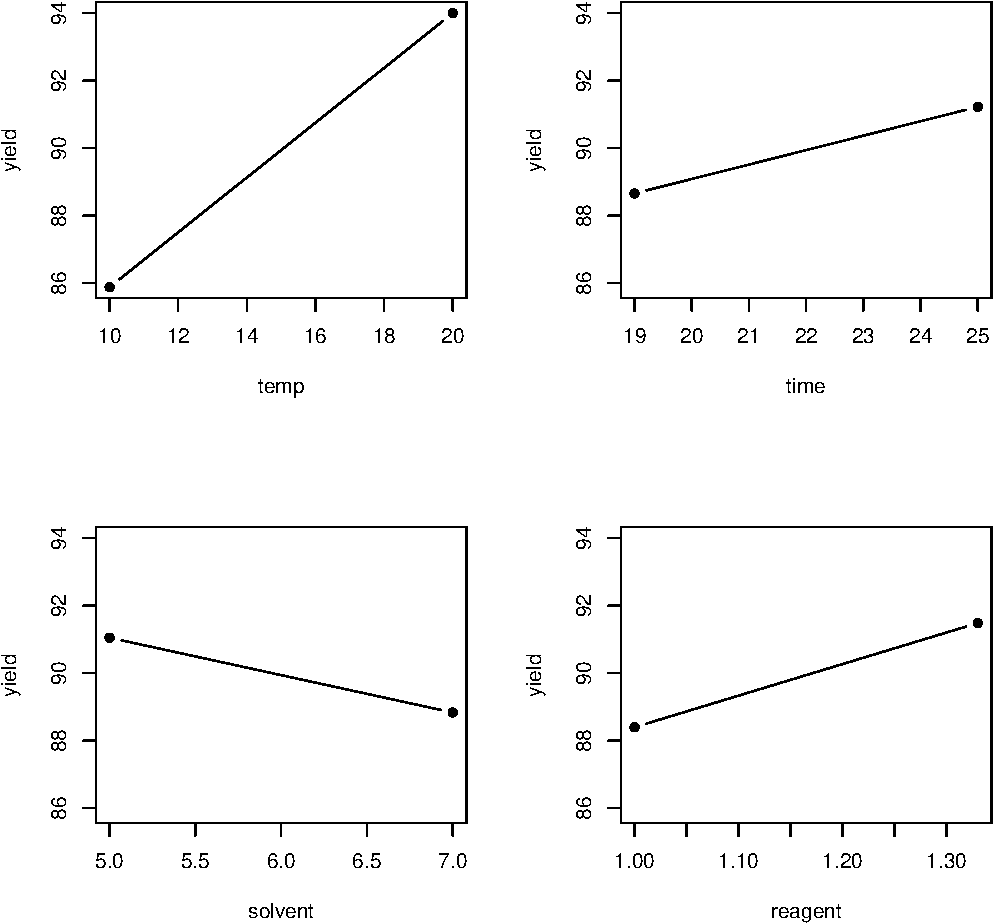
\includegraphics{bookdown_math3014-6027_files/figure-latex/desilylation-me-plots-1} 

}

\caption{Desilylation experiment: main effect plots}\label{fig:desilylation-me-plots}
\end{figure}

\hypertarget{interactions}{%
\subsection{Interactions}\label{interactions}}

Another contrast that could be of interest in Example \ref{exm:factorial-desilylation} has coefficients

\[
\boldsymbol{c}^{\mathrm{T}} = (\boldsymbol{1}_4^{\mathrm{T}}, -\boldsymbol{1}_8^{\mathrm{T}}, \boldsymbol{1}_4^{\mathrm{T}}) / 8\,.
\]
This contrast measures the difference between the average treatment effect from treatments 1-4, 13-16 and treatments 5-12. Checking back against Table \ref{tab:factorial-desilylation-data}, we see this is comparing those treatments where \texttt{solvent} and \texttt{reagent} are both set to their low (1-4) or high (13-16) level against those treatments where one of the two factors is set high and the other is set low (5-12).

Focusing on \texttt{reagent}, if the effect of this factor on the response was independent of the level to which \texttt{solvent} has been set, you would expect this contrast to be zero - changing from the high to low level of \texttt{reagent} should affect the response in the same way, regardless of the setting of \texttt{solvent}. This argument can be reversed, focussing on the effect of \texttt{solvent}. Therefore, if this contrast is large, we say the two factors \textbf{interact}.

\begin{Shaded}
\begin{Highlighting}[]
\NormalTok{sol\_reg\_int.emmc }\OtherTok{\textless{}{-}} \ControlFlowTok{function}\NormalTok{(levels) }
  \FunctionTok{data.frame}\NormalTok{(}\StringTok{\textquotesingle{}reagent x solvent\textquotesingle{}} \OtherTok{=}\NormalTok{ .}\DecValTok{125} \SpecialCharTok{*} \FunctionTok{c}\NormalTok{(}\FunctionTok{rep}\NormalTok{(}\DecValTok{1}\NormalTok{, }\DecValTok{4}\NormalTok{), }\FunctionTok{rep}\NormalTok{(}\SpecialCharTok{{-}}\DecValTok{1}\NormalTok{, }\DecValTok{8}\NormalTok{), }\FunctionTok{rep}\NormalTok{(}\DecValTok{1}\NormalTok{, }\DecValTok{4}\NormalTok{)))}
\NormalTok{emmeans}\SpecialCharTok{::}\FunctionTok{contrast}\NormalTok{(desilylation.emm, }\StringTok{\textquotesingle{}sol\_reg\_int\textquotesingle{}}\NormalTok{)}
\end{Highlighting}
\end{Shaded}

\begin{verbatim}
##  contrast          estimate  SE df t.ratio p.value
##  reagent.x.solvent     0.49 NaN  0     NaN     NaN
\end{verbatim}

For Example \ref{exm:factorial-desilylation}, this interaction contrast seems quite small, although of course without an estimate of the standard error we are still lacking a formal method to judge this.

It is somewhat more informative to consider the above interaction contrast as the average difference in two ``sub-contrasts''

\[
\boldsymbol{c}^{\mathrm{T}}\boldsymbol{\tau} = \frac{1}{2}\left\{\frac{1}{4}\left(\tau_{13} + \tau_{14} + \tau_{15} + \tau_{16} - \tau_5 - \tau_6 - \tau_7 - \tau_8\right)
- \frac{1}{4}\left(\tau_9 + \tau_{10} + \tau_{11} + \tau_{12} - \tau_1 - \tau_2 - \tau_3 - \tau_4\right) \right\}\,,
\]
The first component in the above expression is the effect of changing \texttt{reagent} from high to low \textbf{given \texttt{solvent} is set to it's high level}. The second component the effect of changing \texttt{reagent} from high to low \textbf{given \texttt{solvent} is set to it's low level}. This leads to our definition of a two-factor interaction.

\begin{definition}
\protect\hypertarget{def:two-factor-interaction}{}\label{def:two-factor-interaction}

The \textbf{two-factor interaction} between factors \(A\) and \(B\) is defined as the average difference in main effect of factor \(A\) when computed at the high and low levels of factor \(B\).

\begin{align*}
\mbox{Int}(A, B) & = \frac{1}{2}\left\{\mbox{ME}(A\mid B+) - \mbox{ME}(A \mid B-)\right\} \\
& = \frac{1}{2}\left\{\mbox{ME}(B \mid A+) - \mbox{ME}(B \mid A-)\right\} \\
& = \frac{1}{2}\left\{\bar{y}(A+, B+) - \bar{y}(A-, B+) - \bar{y}(A+, B-) + \bar{y}(A-, B-)\right\}\,,
\end{align*}

where \(\bar{y}(A+, B-)\) is the average response when factor \(A\) is set to its high level and factor \(B\) is set to its low level, averaged across all combinations of levels of the other factors, and other averages are defined similarly. The conditional main effects of factor \(A\) when factor \(B\) is set to its high level is defined as

\[
\mbox{ME}(A\mid B+) = \bar{y}(A+, B+) - \bar{y}(A-, B+)\,,
\]

with similar definitions for other conditional main effects.

\end{definition}

As the sum of the squared contrast coefficients is the same for two-factor interactions as for main effects, the variance of the contrast estimator is also the same.

\[
\mbox{var}\left\{\mbox{Int}(A, B)\right\} = \frac{4\sigma^2}{n}\,.
\]
For Example \ref{exm:factorial-desilylation} we can calculate two-factor interactions for all \({4 \choose 2} = 6\) pairs of factors. The simplest way to calculate the contrast coefficients is as the elementwise, or Hadamard, product\footnote{For two matrices \(A\) and \(B\) of the same dimension \(m\times n\), the Hadamard product \(A\odot B\) is a matrix of the same dimension with elements given by the elementwise product, \((A\odot B)_{ij} = A_{ij}B_{ij}\).} of the unscaled main effect contrasts (before dividing by \(n/2\)).

\begin{Shaded}
\begin{Highlighting}[]
\NormalTok{fac.contrasts.int.emmc }\OtherTok{\textless{}{-}} \ControlFlowTok{function}\NormalTok{(levs) \{}
  \FunctionTok{with}\NormalTok{(}\FunctionTok{sqrt}\NormalTok{(}\DecValTok{8}\NormalTok{) }\SpecialCharTok{*}\NormalTok{ main\_effect\_contrasts, \{}
    \FunctionTok{data.frame}\NormalTok{(}\StringTok{\textquotesingle{}tem\_x\_tim\textquotesingle{}} \OtherTok{=}\NormalTok{ temp }\SpecialCharTok{*}\NormalTok{ time,}
               \StringTok{\textquotesingle{}tem\_x\_sol\textquotesingle{}} \OtherTok{=}\NormalTok{ temp }\SpecialCharTok{*}\NormalTok{ solvent,}
               \StringTok{\textquotesingle{}tem\_x\_rea\textquotesingle{}} \OtherTok{=}\NormalTok{ temp }\SpecialCharTok{*}\NormalTok{ reagent,}
               \StringTok{\textquotesingle{}tim\_x\_sol\textquotesingle{}} \OtherTok{=}\NormalTok{ time }\SpecialCharTok{*}\NormalTok{ solvent,}
               \StringTok{\textquotesingle{}tim\_x\_rea\textquotesingle{}} \OtherTok{=}\NormalTok{ time }\SpecialCharTok{*}\NormalTok{ reagent,}
               \StringTok{\textquotesingle{}sol\_x\_rea\textquotesingle{}} \OtherTok{=}\NormalTok{ solvent }\SpecialCharTok{*}\NormalTok{ reagent)}
\NormalTok{  \})}
\NormalTok{\}}
\NormalTok{two\_fi\_contrasts }\OtherTok{\textless{}{-}} \FunctionTok{fac.contrasts.int.emmc}\NormalTok{()}
\FunctionTok{rownames}\NormalTok{(two\_fi\_contrasts) }\OtherTok{\textless{}{-}} \FunctionTok{paste}\NormalTok{(}\StringTok{"Trt"}\NormalTok{, }\DecValTok{1}\SpecialCharTok{:}\DecValTok{16}\NormalTok{)}
\NormalTok{knitr}\SpecialCharTok{::}\FunctionTok{kable}\NormalTok{(two\_fi\_contrasts, }\AttributeTok{caption =} \StringTok{\textquotesingle{}Desilylation experiment: two{-}factor interaction contrast coefficients\textquotesingle{}}\NormalTok{)}
\end{Highlighting}
\end{Shaded}

\begin{table}

\caption{\label{tab:desilylation-2fi-interactions}Desilylation experiment: two-factor interaction contrast coefficients}
\centering
\begin{tabular}[t]{l|r|r|r|r|r|r}
\hline
  & tem\_x\_tim & tem\_x\_sol & tem\_x\_rea & tim\_x\_sol & tim\_x\_rea & sol\_x\_rea\\
\hline
Trt 1 & 0.125 & 0.125 & 0.125 & 0.125 & 0.125 & 0.125\\
\hline
Trt 2 & -0.125 & -0.125 & -0.125 & 0.125 & 0.125 & 0.125\\
\hline
Trt 3 & -0.125 & 0.125 & 0.125 & -0.125 & -0.125 & 0.125\\
\hline
Trt 4 & 0.125 & -0.125 & -0.125 & -0.125 & -0.125 & 0.125\\
\hline
Trt 5 & 0.125 & -0.125 & 0.125 & -0.125 & 0.125 & -0.125\\
\hline
Trt 6 & -0.125 & 0.125 & -0.125 & -0.125 & 0.125 & -0.125\\
\hline
Trt 7 & -0.125 & -0.125 & 0.125 & 0.125 & -0.125 & -0.125\\
\hline
Trt 8 & 0.125 & 0.125 & -0.125 & 0.125 & -0.125 & -0.125\\
\hline
Trt 9 & 0.125 & 0.125 & -0.125 & 0.125 & -0.125 & -0.125\\
\hline
Trt 10 & -0.125 & -0.125 & 0.125 & 0.125 & -0.125 & -0.125\\
\hline
Trt 11 & -0.125 & 0.125 & -0.125 & -0.125 & 0.125 & -0.125\\
\hline
Trt 12 & 0.125 & -0.125 & 0.125 & -0.125 & 0.125 & -0.125\\
\hline
Trt 13 & 0.125 & -0.125 & -0.125 & -0.125 & -0.125 & 0.125\\
\hline
Trt 14 & -0.125 & 0.125 & 0.125 & -0.125 & -0.125 & 0.125\\
\hline
Trt 15 & -0.125 & -0.125 & -0.125 & 0.125 & 0.125 & 0.125\\
\hline
Trt 16 & 0.125 & 0.125 & 0.125 & 0.125 & 0.125 & 0.125\\
\hline
\end{tabular}
\end{table}

Estimates of the interaction contrasts can again by found by considering the equivalent contrasts in the observed treatment means.

\begin{Shaded}
\begin{Highlighting}[]
\FunctionTok{t}\NormalTok{(}\FunctionTok{as.matrix}\NormalTok{(two\_fi\_contrasts)) }\SpecialCharTok{\%*\%}\NormalTok{ yield}
\end{Highlighting}
\end{Shaded}

\begin{verbatim}
##             [,1]
## tem_x_tim -2.357
## tem_x_sol  2.358
## tem_x_rea -2.773
## tim_x_sol  0.440
## tim_x_rea -0.645
## sol_x_rea  0.490
\end{verbatim}

\begin{Shaded}
\begin{Highlighting}[]
\NormalTok{emmeans}\SpecialCharTok{::}\FunctionTok{contrast}\NormalTok{(desilylation.emm, }\StringTok{\textquotesingle{}fac.contrasts.int\textquotesingle{}}\NormalTok{)}
\end{Highlighting}
\end{Shaded}

\begin{verbatim}
##  contrast  estimate  SE df t.ratio p.value
##  tem_x_tim   -2.357 NaN  0     NaN     NaN
##  tem_x_sol    2.357 NaN  0     NaN     NaN
##  tem_x_rea   -2.772 NaN  0     NaN     NaN
##  tim_x_sol    0.440 NaN  0     NaN     NaN
##  tim_x_rea   -0.645 NaN  0     NaN     NaN
##  sol_x_rea    0.490 NaN  0     NaN     NaN
\end{verbatim}

As with main effects, interactions are often displayed graphically using \textbf{interaction} plots, plotting average responses for each pairwise combination of factors, joined by lines.

\begin{Shaded}
\begin{Highlighting}[]
\NormalTok{plotmin }\OtherTok{\textless{}{-}} \FunctionTok{min}\NormalTok{(desilylation}\SpecialCharTok{$}\NormalTok{yield)}
\NormalTok{plotmax }\OtherTok{\textless{}{-}} \FunctionTok{max}\NormalTok{(desilylation}\SpecialCharTok{$}\NormalTok{yield)}
\FunctionTok{par}\NormalTok{(}\AttributeTok{cex =} \DecValTok{2}\NormalTok{)}
\FunctionTok{layout}\NormalTok{(}\FunctionTok{matrix}\NormalTok{(}\FunctionTok{c}\NormalTok{(}\DecValTok{1}\NormalTok{, }\DecValTok{2}\NormalTok{, }\DecValTok{3}\NormalTok{, }\DecValTok{4}\NormalTok{, }\DecValTok{5}\NormalTok{, }\DecValTok{6}\NormalTok{), }\AttributeTok{nrow =} \DecValTok{3}\NormalTok{, }\AttributeTok{ncol =} \DecValTok{2}\NormalTok{, }\AttributeTok{byrow =} \ConstantTok{TRUE}\NormalTok{), }\AttributeTok{respect =}\NormalTok{ T)}

\FunctionTok{with}\NormalTok{(desilylation, \{}
  \FunctionTok{interaction.plot}\NormalTok{(temp, time, yield, }\AttributeTok{type =} \StringTok{"b"}\NormalTok{, }\AttributeTok{pch =} \DecValTok{16}\NormalTok{, }\AttributeTok{legend =}\NormalTok{ F, }
                   \AttributeTok{ylim =} \FunctionTok{c}\NormalTok{(plotmin, plotmax))}
  \FunctionTok{legend}\NormalTok{(}\StringTok{"bottomright"}\NormalTok{, }\AttributeTok{legend =} \FunctionTok{c}\NormalTok{(}\StringTok{"Time = 19"}\NormalTok{, }\StringTok{"Time = 25"}\NormalTok{), }\AttributeTok{lty =} \DecValTok{2}\SpecialCharTok{:}\DecValTok{1}\NormalTok{, }\AttributeTok{cex =}\NormalTok{ .}\DecValTok{75}\NormalTok{)}
  \FunctionTok{interaction.plot}\NormalTok{(temp, solvent, yield, }\AttributeTok{type =} \StringTok{"b"}\NormalTok{, }\AttributeTok{pch =} \DecValTok{16}\NormalTok{, }\AttributeTok{legend =}\NormalTok{ F, }
                   \AttributeTok{ylim =} \FunctionTok{c}\NormalTok{(plotmin, plotmax))}
  \FunctionTok{legend}\NormalTok{(}\StringTok{"bottomright"}\NormalTok{, }\AttributeTok{legend =} \FunctionTok{c}\NormalTok{(}\StringTok{"Solvent = 5"}\NormalTok{, }\StringTok{"Solvent = 7"}\NormalTok{), }\AttributeTok{lty =} \DecValTok{2}\SpecialCharTok{:}\DecValTok{1}\NormalTok{, }\AttributeTok{cex =}\NormalTok{ .}\DecValTok{75}\NormalTok{)}
  \FunctionTok{interaction.plot}\NormalTok{(temp, reagent, yield, }\AttributeTok{type =} \StringTok{"b"}\NormalTok{, }\AttributeTok{pch =} \DecValTok{16}\NormalTok{, }\AttributeTok{legend =}\NormalTok{ F, }
                   \AttributeTok{ylim =} \FunctionTok{c}\NormalTok{(plotmin, plotmax))}
  \FunctionTok{legend}\NormalTok{(}\StringTok{"bottomright"}\NormalTok{, }\AttributeTok{legend =} \FunctionTok{c}\NormalTok{(}\StringTok{"Reagent = 1"}\NormalTok{, }\StringTok{"Reagent = 1.33"}\NormalTok{), }\AttributeTok{lty =} \DecValTok{2}\SpecialCharTok{:}\DecValTok{1}\NormalTok{, }\AttributeTok{cex =}\NormalTok{ .}\DecValTok{75}\NormalTok{)}
  \FunctionTok{interaction.plot}\NormalTok{(time, solvent, yield, }\AttributeTok{type =} \StringTok{"b"}\NormalTok{, }\AttributeTok{pch =} \DecValTok{16}\NormalTok{, }\AttributeTok{legend =}\NormalTok{ F, }
                   \AttributeTok{ylim =} \FunctionTok{c}\NormalTok{(plotmin, plotmax))}
  \FunctionTok{legend}\NormalTok{(}\StringTok{"bottomright"}\NormalTok{, }\AttributeTok{legend =} \FunctionTok{c}\NormalTok{(}\StringTok{"Solvent = 5"}\NormalTok{, }\StringTok{"Solvent = 7"}\NormalTok{), }\AttributeTok{lty =} \DecValTok{2}\SpecialCharTok{:}\DecValTok{1}\NormalTok{, }\AttributeTok{cex =}\NormalTok{ .}\DecValTok{75}\NormalTok{)}
  \FunctionTok{interaction.plot}\NormalTok{(time, reagent, yield, }\AttributeTok{type =} \StringTok{"b"}\NormalTok{, }\AttributeTok{pch =} \DecValTok{16}\NormalTok{, }\AttributeTok{legend =}\NormalTok{ F, }
                   \AttributeTok{ylim =} \FunctionTok{c}\NormalTok{(plotmin, plotmax))}
  \FunctionTok{legend}\NormalTok{(}\StringTok{"bottomright"}\NormalTok{, }\AttributeTok{legend =} \FunctionTok{c}\NormalTok{(}\StringTok{"Reagent = 1"}\NormalTok{, }\StringTok{"Reagent = 1.33"}\NormalTok{), }\AttributeTok{lty =} \DecValTok{2}\SpecialCharTok{:}\DecValTok{1}\NormalTok{, }\AttributeTok{cex =}\NormalTok{ .}\DecValTok{75}\NormalTok{)}
  \FunctionTok{interaction.plot}\NormalTok{(solvent, reagent, yield, }\AttributeTok{type =} \StringTok{"b"}\NormalTok{, }\AttributeTok{pch =} \DecValTok{16}\NormalTok{, }\AttributeTok{legend =}\NormalTok{ F, }
                   \AttributeTok{ylim =} \FunctionTok{c}\NormalTok{(plotmin, plotmax))}
  \FunctionTok{legend}\NormalTok{(}\StringTok{"bottomright"}\NormalTok{, }\AttributeTok{legend =} \FunctionTok{c}\NormalTok{(}\StringTok{"Reagent = 1"}\NormalTok{, }\StringTok{"Reagent = 1.33"}\NormalTok{), }\AttributeTok{lty =} \DecValTok{2}\SpecialCharTok{:}\DecValTok{1}\NormalTok{, }\AttributeTok{cex =}\NormalTok{ .}\DecValTok{75}\NormalTok{)}
\NormalTok{\})}
\end{Highlighting}
\end{Shaded}

\begin{figure}

{\centering 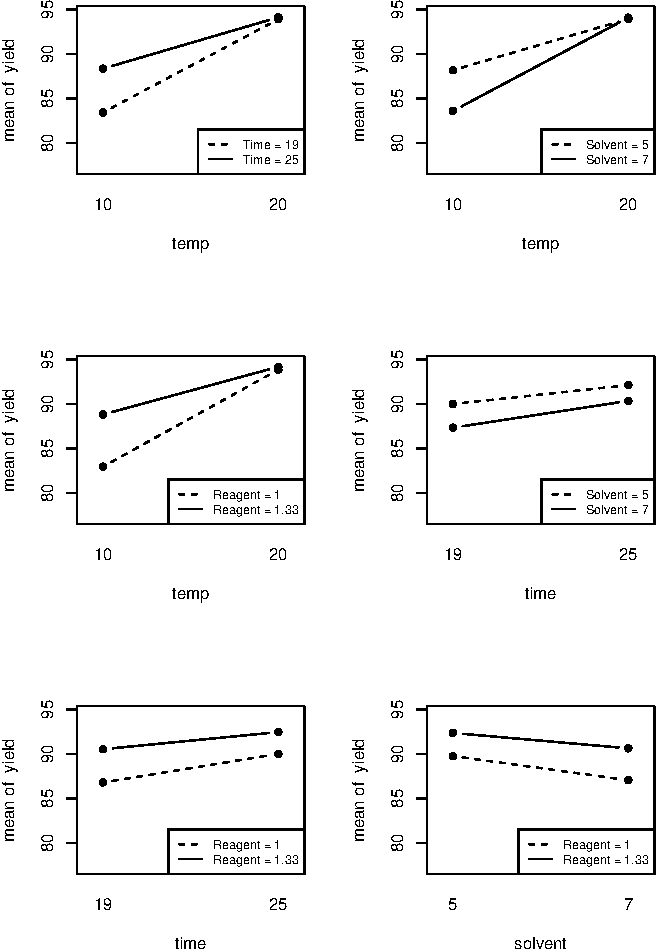
\includegraphics{bookdown_math3014-6027_files/figure-latex/desilylation-2fi-plots-1} 

}

\caption{Desilylation experiment: two-factor interaction plots}\label{fig:desilylation-2fi-plots}
\end{figure}

Parallel lines in an interaction plot indicate no (or very small) interaction (\texttt{time} and \texttt{solvent}, \texttt{time} and \texttt{reagent}, \texttt{solvent} and \texttt{reagent}). The three interactions with \texttt{temp} all demonstrate much more robust behaviour at the high level; changing \texttt{time}, \texttt{solvent} or \texttt{reagent} makes little difference to the response at the high level of \texttt{temp}, and much less difference than at the low level of \texttt{temp}.

If a system displays important interactions, the main effects of factors involved in those interactions should no longer be interpreted. For example, it makes little sense to discuss the main effect of \texttt{temp} when is changes so much with the level of \texttt{reagent} (from strongly positive when \texttt{reagent} is low to quite small when \texttt{reagent} is high).

Higher order interactions can be defined similarly, as average differences in lower-order effects. For example, a three-factor interaction measures how a two-factor interaction changes with the levels of a third factor.

\begin{align*}
\mbox{Int}(A, B, C) & = \frac{1}{2}\left\{\mbox{Int}(A, B \mid C+) - \mbox{Int}(A, B \mid C-)\right\} \\
& = \frac{1}{2}\left\{\mbox{Int}(A, C \mid B+) - \mbox{Int}(A, C \mid B-)\right\} \\
& = \frac{1}{2}\left\{\mbox{Int}(B, C \mid A+) - \mbox{Int}(B, C \mid A-)\right\}\,, \\
\end{align*}

where

\[
\mbox{Int}(A, B \mid C+) = \frac{1}{2}\left\{\bar{y}(A+, B+, C+) - \bar{y}(A-, B+, C+) - \bar{y}(A+, B-, C+) + \bar{y}(A-, B-, C+)\right\}
\]
is the interaction between factors \(A\) and \(B\) using only those treatments where factor \(C\) is set to it's high level. Higher order interaction contrasts can again be constructed by (multiple) hadamard products of (unscaled) main effect contrasts.

\begin{definition}
\protect\hypertarget{def:factorial-effects}{}\label{def:factorial-effects}

A \textbf{factorial effect} is a main effect or interaction contrast defined on a factorial experiment. For a \(2^f\) factorial experiment with \(f\) factors, there are \(2^f-1\) factorial effects, ranging from main effects to the interaction between all \(f\) factors.

\end{definition}

For Example \ref{exm:factorial-desilylation}, we can now calculate all the factorial effects.

\begin{Shaded}
\begin{Highlighting}[]
\DocumentationTok{\#\# hadamard products}
\NormalTok{unscaled\_me\_contrasts }\OtherTok{\textless{}{-}} \DecValTok{8} \SpecialCharTok{*}\NormalTok{ main\_effect\_contrasts}
\NormalTok{factorial\_contrasts }\OtherTok{\textless{}{-}} \FunctionTok{model.matrix}\NormalTok{(}\SpecialCharTok{\textasciitilde{}}\NormalTok{.}\SpecialCharTok{\^{}}\DecValTok{4}\NormalTok{, unscaled\_me\_contrasts)[, }\SpecialCharTok{{-}}\DecValTok{1}\NormalTok{] }\SpecialCharTok{/} \DecValTok{8}

\DocumentationTok{\#\# all factorial effects {-} directly, as there is no treatment replication}
\FunctionTok{t}\NormalTok{(factorial\_contrasts) }\SpecialCharTok{\%*\%}\NormalTok{ yield}
\end{Highlighting}
\end{Shaded}

\begin{verbatim}
##                              [,1]
## temp                       8.1200
## time                       2.5675
## solvent                   -2.2175
## reagent                    3.0875
## temp:time                 -2.3575
## temp:solvent               2.3575
## temp:reagent              -2.7725
## time:solvent               0.4400
## time:reagent              -0.6450
## solvent:reagent            0.4900
## temp:time:solvent          0.2450
## temp:time:reagent          0.1950
## temp:solvent:reagent      -0.0300
## time:solvent:reagent      -0.2375
## temp:time:solvent:reagent  0.1925
\end{verbatim}

\begin{Shaded}
\begin{Highlighting}[]
\DocumentationTok{\#\# using emmeans}
\NormalTok{factorial\_contrasts.emmc }\OtherTok{\textless{}{-}} \ControlFlowTok{function}\NormalTok{(levs) }\FunctionTok{data.frame}\NormalTok{(factorial\_contrasts)}
\NormalTok{desilylation.effs }\OtherTok{\textless{}{-}}\NormalTok{ emmeans}\SpecialCharTok{::}\FunctionTok{contrast}\NormalTok{(desilylation.emm, }\StringTok{\textquotesingle{}factorial\_contrasts\textquotesingle{}}\NormalTok{)}
\NormalTok{desilylation.effs}
\end{Highlighting}
\end{Shaded}

\begin{verbatim}
##  contrast                  estimate  SE df t.ratio p.value
##  temp                         8.120 NaN  0     NaN     NaN
##  time                         2.567 NaN  0     NaN     NaN
##  solvent                     -2.218 NaN  0     NaN     NaN
##  reagent                      3.087 NaN  0     NaN     NaN
##  temp.time                   -2.357 NaN  0     NaN     NaN
##  temp.solvent                 2.358 NaN  0     NaN     NaN
##  temp.reagent                -2.772 NaN  0     NaN     NaN
##  time.solvent                 0.440 NaN  0     NaN     NaN
##  time.reagent                -0.645 NaN  0     NaN     NaN
##  solvent.reagent              0.490 NaN  0     NaN     NaN
##  temp.time.solvent            0.245 NaN  0     NaN     NaN
##  temp.time.reagent            0.195 NaN  0     NaN     NaN
##  temp.solvent.reagent        -0.030 NaN  0     NaN     NaN
##  time.solvent.reagent        -0.238 NaN  0     NaN     NaN
##  temp.time.solvent.reagent    0.193 NaN  0     NaN     NaN
\end{verbatim}

\hypertarget{fact-principles}{%
\section{Three principles for factorial effects}\label{fact-principles}}

Empirical study of many experiments \citep{BoxMeyer1986, Li2006} have demonstrated that the following three principles \textbf{often} hold when analysing factorial experiments.

\begin{definition}
\protect\hypertarget{def:effect-hierarchy}{}\label{def:effect-hierarchy}

\textbf{Effect hierarchy}: lower-order factorial effects are more likely to be important than higher-order effects; factorial effects of the same order are equally likely to be important.

For example, we would anticipate more large main effects from the analysis of a factorial experiment than two-factor interactions.

\end{definition}

\begin{definition}
\protect\hypertarget{def:effect-sparsity}{}\label{def:effect-sparsity}

\textbf{Effect sparsity}: the number of large factorial effects is likely to be small, relative to the total number under study.

This is sometimes called the \textbf{pareto principle}.

\end{definition}

\begin{definition}
\protect\hypertarget{def:effect-heredity}{}\label{def:effect-heredity}

\textbf{Effect heredity}: interactions are more likely to be important if at least one parent factor also has a large main effect.

\end{definition}

These three principles will provide us with some useful guidelines when analysing, and eventually constructing, factorial experiments.

\hypertarget{unreplicated-normal-plots}{%
\section{Normal effect plots for unreplicated factorial designs}\label{unreplicated-normal-plots}}

The lack of an estmate for \(\sigma^2\) means alternatives to formal inference methods (e.g.~hypothesis tests) must be found to assess the size of factorial effects. We will discuss a method that essentially treats the identification of large factorial effects as an outlier identification problem.

Let \(\hat{\theta}_j\) be the \(j\)th estimated factorial effect, with \(\hat{\theta}_j = \sum_{i=1}^tc_{ij}\bar{y}_{i.}\) for \(\boldsymbol{c}_j^{\mathrm{T}} = (c_{1j}, \ldots, c_{tj})\) a vector of factorial contrast coefficients (defining a main effect or interaction). Then the estimator follows a normal distribution

\[
\hat{\theta}_j \sim N\left(\theta_j, \frac{4\sigma^2}{n}\right)\,,\qquad j = 1, \ldots, 2^f-1\,,
\]
for \(\theta_j\) the true, unknown, value of the factorial effect, \(j = 1,\ldots, 2^f\). Further more, for \(j, l = 1, \ldots 2^f-1; \, j\ne l\),

\begin{align*}
\mbox{cov}(\hat{\theta}_j, \hat{\theta}_l) & =  \mbox{cov}\left(\sum_{i=1}^tc_{ij}\bar{y}_{i.}, \sum_{i=1}^tc_{il}\bar{y}_{i.}\right) \\
& = \sum_{i=1}^tc_{ij}c_{il}\mbox{var}(\bar{y}_{i.}) \\
& = \frac{\sigma^2}{r} \sum_{i=1}^tc_{ij}c_{il} \\
& = 0\,, \\
\end{align*}

as \(\sum_{i=1}^tc_{ij}c_{il} = 0\) for \(j\ne l\). That is, the factorial contrasts are independent as the contrast coefficient vectors are orthogonal.

Hence, under the null hypothesis \(H_0: \theta_1 = \cdots = \theta_{2^f-1} = 0\) (all factorial effects are zero), the \(\hat{\theta}_j\) form a sample from \textbf{independent} normally distributed random variables from the distribution

\begin{equation}
\hat{\theta}_j \sim N\left(0, \frac{4\sigma^2}{n}\right)\,,\qquad j = 1, \ldots, 2^f-1\,.
\label{eq:npph0}
\end{equation}

To assess evidence against \(H_0\), we can plot the ordered estimates of the factorial effects against the ordered quantiles of a standard normal distribution. Under \(H_0\), the points in this plot should lie on a straightline (the slope of the line will depend on the unknown \(\sigma^2\)). We anticipate that the majority of the effects will be small (\emph{effect sparsity}), and hence any large effects that lie away from the line are unlikely to come from distribution \eqref{eq:npph0} and may be significantly different from zero. We have essentially turned the problem into an outlier identification problem.

For Example \ref{exm:factorial-desilylation}, we can easily produce this plot in \texttt{R}. Table \ref{tab:desilylation-effects-plot1} gives the ordered factorial effects, which are then plotted against standard normal quantiles in Figure \ref{fig:desilylation-effects-plot1}.

\begin{Shaded}
\begin{Highlighting}[]
\NormalTok{effs }\OtherTok{\textless{}{-}}\NormalTok{ dplyr}\SpecialCharTok{::}\FunctionTok{arrange}\NormalTok{(}\FunctionTok{transform}\NormalTok{(desilylation.effs)[,}\DecValTok{1}\SpecialCharTok{:}\DecValTok{2}\NormalTok{], dplyr}\SpecialCharTok{::}\FunctionTok{desc}\NormalTok{(estimate))}
\NormalTok{knitr}\SpecialCharTok{::}\FunctionTok{kable}\NormalTok{(effs, }\AttributeTok{caption =} \StringTok{"Desilylation experiment: sorted estimated factorial effects"}\NormalTok{)}
\FunctionTok{qqnorm}\NormalTok{(effs[ ,}\DecValTok{2}\NormalTok{], }\AttributeTok{ylab =} \StringTok{"Factorial effects"}\NormalTok{, }\AttributeTok{main =} \StringTok{""}\NormalTok{) }\CommentTok{\# note that qqnorm/qqline/qqplot don\textquotesingle{}t require sorted data}
\FunctionTok{qqline}\NormalTok{(effs[ ,}\DecValTok{2}\NormalTok{])}
\end{Highlighting}
\end{Shaded}

\begin{table}

\caption{\label{tab:desilylation-effects-plot1}Desilylation experiment: sorted estimated factorial effects}
\centering
\begin{tabular}[t]{l|r}
\hline
contrast & estimate\\
\hline
temp & 8.1200\\
\hline
reagent & 3.0875\\
\hline
time & 2.5675\\
\hline
temp.solvent & 2.3575\\
\hline
solvent.reagent & 0.4900\\
\hline
time.solvent & 0.4400\\
\hline
temp.time.solvent & 0.2450\\
\hline
temp.time.reagent & 0.1950\\
\hline
temp.time.solvent.reagent & 0.1925\\
\hline
temp.solvent.reagent & -0.0300\\
\hline
time.solvent.reagent & -0.2375\\
\hline
time.reagent & -0.6450\\
\hline
solvent & -2.2175\\
\hline
temp.time & -2.3575\\
\hline
temp.reagent & -2.7725\\
\hline
\end{tabular}
\end{table}

\begin{figure}

{\centering 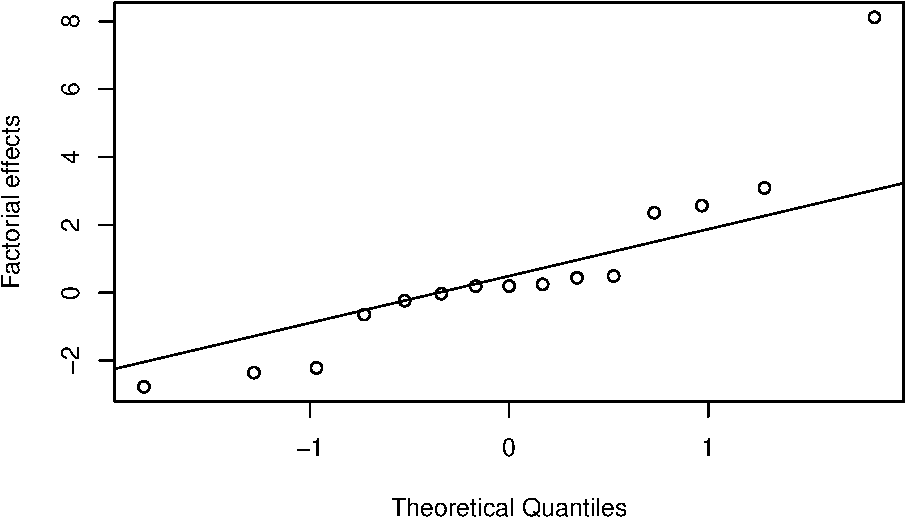
\includegraphics{bookdown_math3014-6027_files/figure-latex/desilylation-effects-plot1-1} 

}

\caption{Desilylation experiment: normal effects plot}\label{fig:desilylation-effects-plot1}
\end{figure}

In fact, it is more usual to use a \textbf{half-normal} plot to assess the size of factorial effects, where we plot the sorted absolute values of the estimated effects against the quantiles of a half-normal distribution\footnote{The absolute value of a normally distributed random variable follows a half-normal distribution.}

\begin{Shaded}
\begin{Highlighting}[]
\NormalTok{p }\OtherTok{\textless{}{-}}\NormalTok{ .}\DecValTok{5} \SpecialCharTok{+}\NormalTok{ .}\DecValTok{5} \SpecialCharTok{*}\NormalTok{ (}\DecValTok{1}\SpecialCharTok{:}\DecValTok{16} \SpecialCharTok{{-}}\NormalTok{ .}\DecValTok{5}\NormalTok{) }\SpecialCharTok{/}\DecValTok{16} \CommentTok{\# probabilities we will plot against}
\FunctionTok{qqplot}\NormalTok{(}\AttributeTok{x =} \FunctionTok{qnorm}\NormalTok{(p), }\AttributeTok{y =} \FunctionTok{abs}\NormalTok{(effs[,}\DecValTok{2}\NormalTok{]), }\AttributeTok{ylab =} \StringTok{"Absolute factorial effects"}\NormalTok{, }
       \AttributeTok{xlab =} \StringTok{"Half{-}normal quantiles"}\NormalTok{)}
\end{Highlighting}
\end{Shaded}

\begin{figure}

{\centering 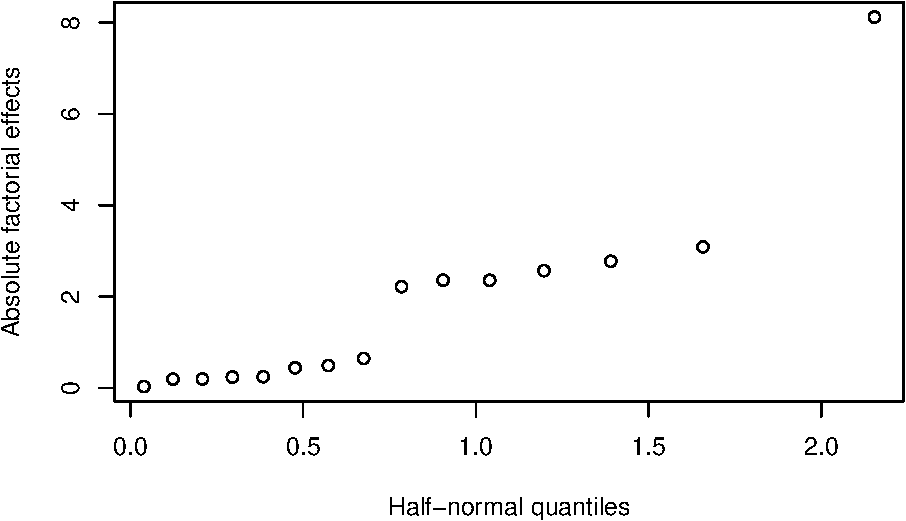
\includegraphics{bookdown_math3014-6027_files/figure-latex/desilylation-half-normal-plot-1} 

}

\caption{Desilylation experiment: half-normal effects plot}\label{fig:desilylation-half-normal-plot}
\end{figure}

The advantage of a half-normal plot such as Figure \ref{fig:desilylation-half-normal-plot} is that we only need to look at effects appearing in the top right corner (significant effects will always appear ``above'' a hypothetical straight line) and we do not need to worry about comparing large positive and negative values. For these reason, they are usually preferred over normal plots.

For the desilylation experiment, we can see the effects fall into three groups: one effect standing well away from the line, and almost certainly significant (\texttt{temp}, from Table \ref{desilylation-effects-plot1}), then a group of six effects (\texttt{reagent}, \texttt{time}, \texttt{temp.solvent}, \texttt{solvent}, \texttt{temp.time}, \texttt{temp.reagent}) which may be significant, and then a group of 8 much smaller effects.

\hypertarget{lenths-method-for-approximate-hypothesis-testing}{%
\subsection{Lenth's method for approximate hypothesis testing}\label{lenths-method-for-approximate-hypothesis-testing}}

The assessment of normal or half-normal effect plots can be quite subjective. \citet{Lenth1989} introduced a simple method for conducting more formal hypothesis testing in unreplicated factorial experiments.

Lenth's method uses a \textbf{pseudo standard error} (PSE):

\[
\mbox{PSE} = 1.5 \times \mbox{median}_{|\hat{\theta}_i| < 2.5s_0}|\hat{\theta}_i|\,,
\]
where \(s_0 = 1.5\times \mbox{median} |\hat{\theta}_i|\) is a \emph{consistent}\footnote{Essentially, \(s_0\) tends in probability to \(\sigma\) as the number of factorial effects tends to infinity.} estimator of the standard deviation of the \(\hat{\theta}_i\) under \(H_0: \theta_1 = \cdots=\theta_{2^f-1}=0\). The PSE trims approximately 1\%\footnote{Under \(H_0\), the \(\hat{\theta}_i\) come from a mean-zero normal distribution, and about 1\% of deviates fall outside \(\pm 2.57\sigma^2\).} of the \(\hat{\theta}_i\) to produce a \textbf{robust} estimator of the standard deviation, in the sense that it is not influenced by large \(\hat{\theta}_i\) belonging to important effects.

For Example \ref{exm:factorial-desilylation}, we can construct the PSE as follows.

\begin{Shaded}
\begin{Highlighting}[]
\NormalTok{s0 }\OtherTok{\textless{}{-}} \FloatTok{1.5} \SpecialCharTok{*} \FunctionTok{median}\NormalTok{(}\FunctionTok{abs}\NormalTok{(effs[, }\DecValTok{2}\NormalTok{]))}
\NormalTok{trimmed }\OtherTok{\textless{}{-}} \FunctionTok{abs}\NormalTok{(effs[, }\DecValTok{2}\NormalTok{]) }\SpecialCharTok{\textless{}} \FloatTok{2.5} \SpecialCharTok{*}\NormalTok{ s0}
\NormalTok{pse }\OtherTok{\textless{}{-}} \FloatTok{1.5} \SpecialCharTok{*} \FunctionTok{median}\NormalTok{(}\FunctionTok{abs}\NormalTok{(effs[trimmed, }\DecValTok{2}\NormalTok{]))}
\NormalTok{pse}
\end{Highlighting}
\end{Shaded}

\begin{verbatim}
## [1] 0.66
\end{verbatim}

The PSE can be used to construct test statistics

\[
t_{\mbox{PSE}, i} = \frac{\hat{\theta}_i}{\mbox{PSE}}\,,
\]

which mimic the usual \(t\)-statistics used when an estimate of \(\sigma^2\) is available. These quantities can be compared to reference distribution which was tabulated by \citet{Lenth1989} and simulated in \texttt{R} using the \texttt{unrepx} package.

\begin{Shaded}
\begin{Highlighting}[]
\NormalTok{eff\_est }\OtherTok{\textless{}{-}}\NormalTok{ effs[, }\DecValTok{2}\NormalTok{]}
\FunctionTok{names}\NormalTok{(eff\_est) }\OtherTok{\textless{}{-}}\NormalTok{ effs[, }\DecValTok{1}\NormalTok{]}
\NormalTok{lenth\_tests }\OtherTok{\textless{}{-}}\NormalTok{ unrepx}\SpecialCharTok{::}\FunctionTok{eff.test}\NormalTok{(eff\_est, }\AttributeTok{method =} \StringTok{"Lenth"}\NormalTok{)}
\NormalTok{knitr}\SpecialCharTok{::}\FunctionTok{kable}\NormalTok{(lenth\_tests, }\AttributeTok{caption =} \StringTok{"Desilylation experiment: hypothesis tests using Lenth\textquotesingle{}s method."}\NormalTok{)}
\end{Highlighting}
\end{Shaded}

\begin{table}

\caption{\label{tab:desilylation-lenth}Desilylation experiment: hypothesis tests using Lenth's method.}
\centering
\begin{tabular}[t]{l|r|r|r|r|r}
\hline
  & effect & Lenth\_PSE & t.ratio & p.value & simult.pval\\
\hline
temp & 8.1200 & 0.66 & 12.303 & 0.0001 & 0.0007\\
\hline
reagent & 3.0875 & 0.66 & 4.678 & 0.0041 & 0.0337\\
\hline
temp.reagent & -2.7725 & 0.66 & -4.201 & 0.0061 & 0.0495\\
\hline
time & 2.5675 & 0.66 & 3.890 & 0.0078 & 0.0652\\
\hline
temp.solvent & 2.3575 & 0.66 & 3.572 & 0.0111 & 0.0945\\
\hline
temp.time & -2.3575 & 0.66 & -3.572 & 0.0111 & 0.0945\\
\hline
solvent & -2.2175 & 0.66 & -3.360 & 0.0135 & 0.1189\\
\hline
time.reagent & -0.6450 & 0.66 & -0.977 & 0.3049 & 0.9955\\
\hline
solvent.reagent & 0.4900 & 0.66 & 0.742 & 0.4312 & 1.0000\\
\hline
time.solvent & 0.4400 & 0.66 & 0.667 & 0.5393 & 1.0000\\
\hline
temp.time.solvent & 0.2450 & 0.66 & 0.371 & 0.7348 & 1.0000\\
\hline
time.solvent.reagent & -0.2375 & 0.66 & -0.360 & 0.7425 & 1.0000\\
\hline
temp.time.reagent & 0.1950 & 0.66 & 0.295 & 0.7848 & 1.0000\\
\hline
temp.time.solvent.reagent & 0.1925 & 0.66 & 0.292 & 0.7875 & 1.0000\\
\hline
temp.solvent.reagent & -0.0300 & 0.66 & -0.045 & 0.9678 & 1.0000\\
\hline
\end{tabular}
\end{table}

The function \texttt{eff.test} calculates unadjusted p-values (\texttt{p.value}) and simultaneous p-values (\texttt{simult.pval}) adjusted to account for multiple testing. Using the latter, from Table \ref{tab:desilylation-lenth} we see that the main effects of \texttt{temp} and \texttt{reagent} are significant at the experiment-wise 5\% level and, obeying \textbf{effect heredity}, their interaction (the p-value is borderline, and hovers around 0.05 depending on simulation error).

The package \texttt{unrepx} also provides the function \texttt{hnplot} to display these results graphically by adding a reference line to a half-normal plot; see Figure \ref{fig:desilylation-lenth-plot}. The \texttt{ME} and \texttt{SME} lines indicate the absolute size of effects that would be required to reject \(H_0: \theta_i = 0\) at an individual or experimentwise \(100\alpha\)\% level, respectively.

\begin{Shaded}
\begin{Highlighting}[]
\NormalTok{unrepx}\SpecialCharTok{::}\FunctionTok{hnplot}\NormalTok{(eff\_est, }\AttributeTok{method =} \StringTok{"Lenth"}\NormalTok{, }\AttributeTok{horiz =}\NormalTok{ F, }\AttributeTok{ID =} \FloatTok{2.7}\NormalTok{, }\AttributeTok{alpha =} \FloatTok{0.05}\NormalTok{)}
\end{Highlighting}
\end{Shaded}

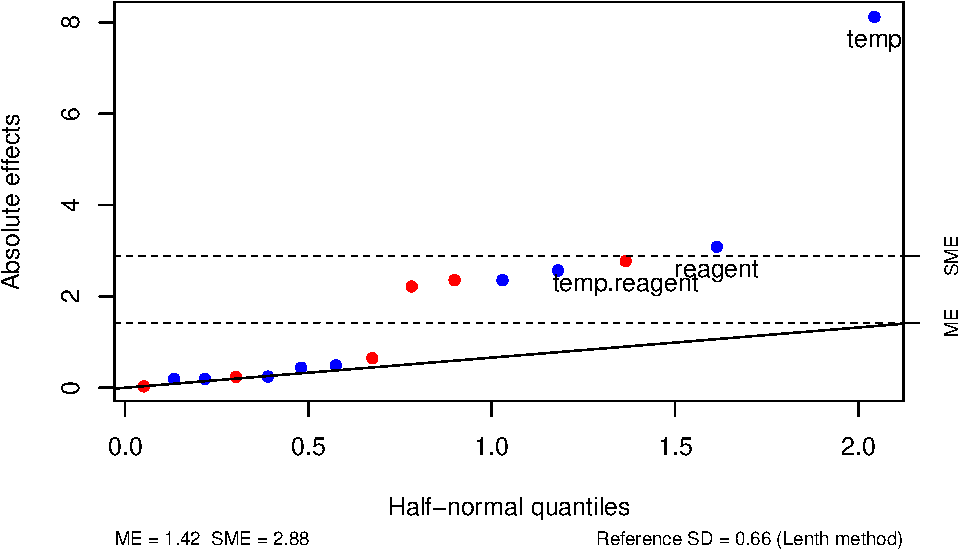
\includegraphics{bookdown_math3014-6027_files/figure-latex/desilylation-lenth-plot-1.pdf}
Informally, factorial effects with estimates greater than \texttt{SME} are thought highly likely to be significant, and effects between \texttt{ME} and \texttt{SME} are considered somewhat likely to be significant (and still worthy of further investigation if the budget allows).

\hypertarget{fac-reg}{%
\section{Regression modelling for factorial experiments}\label{fac-reg}}

We have identified \(d = 2^f-1\) factorial effects that we wish to estimate from our experiment. As \(d < t = 2^f\), we can estimate these factorial effects using a full-rank linear regression model.

Let \(t\times d\) matrix \(C\) hold each factorial contrast as a column. Then

\[
\hat{\boldsymbol{\theta}} = C^{\mathrm{T}}\bar{\boldsymbol{y}}\,,
\]

with \(\hat{\boldsymbol{\theta}}^{\mathrm{T}} = (\hat{\theta}_1, \ldots, \hat{\theta}_d)\) being the vector of estimated factorial effects and \(\bar{\boldsymbol{y}}^{\mathrm{T}} = (\bar{y}_{1.}, \ldots, \bar{y}_{t.})\) being the vector of treatment means.

We can define an \(n\times d\) expanded contrast matrix as \(\tilde{C} = C \otimes \boldsymbol{1}_r\), where each row of \(\tilde{C}\) gives the contrast coefficients for each run of the experiment. Then,

\[
\hat{\boldsymbol{\theta}} = \frac{1}{r}\tilde{C}^{\mathrm{T}}\boldsymbol{y}\,.
\]
To illustrate, we will imagine a hypothetical version of Example \ref{exm:factorial-desilylation} where each treatment was repeated three times (with \(y_{i1} = y_{i2} = y_{i3}\)).

\begin{Shaded}
\begin{Highlighting}[]
\NormalTok{y }\OtherTok{\textless{}{-}} \FunctionTok{kronecker}\NormalTok{(desilylation}\SpecialCharTok{$}\NormalTok{yield, }\FunctionTok{rep}\NormalTok{(}\DecValTok{1}\NormalTok{, }\DecValTok{3}\NormalTok{)) }\CommentTok{\# hypothetical response vector}
\NormalTok{C }\OtherTok{\textless{}{-}}\NormalTok{ factorial\_contrasts}
\NormalTok{Ctilde }\OtherTok{\textless{}{-}} \FunctionTok{kronecker}\NormalTok{(C, }\FunctionTok{rep}\NormalTok{(}\DecValTok{1}\NormalTok{, }\DecValTok{3}\NormalTok{))}
\FunctionTok{t}\NormalTok{(Ctilde) }\SpecialCharTok{\%*\%}\NormalTok{ y }\SpecialCharTok{/} \DecValTok{3} \CommentTok{\# to check}
\end{Highlighting}
\end{Shaded}

\begin{verbatim}
##          [,1]
##  [1,]  8.1200
##  [2,]  2.5675
##  [3,] -2.2175
##  [4,]  3.0875
##  [5,] -2.3575
##  [6,]  2.3575
##  [7,] -2.7725
##  [8,]  0.4400
##  [9,] -0.6450
## [10,]  0.4900
## [11,]  0.2450
## [12,]  0.1950
## [13,] -0.0300
## [14,] -0.2375
## [15,]  0.1925
\end{verbatim}

If we define a model matrix \(X = \frac{2^{f}}{2}\tilde{C}\), then \(X\) is a \(n\times d\) matrix with entries \(\pm 1\) and columns equal to unscaled factorial contrasts. Then

\begin{align}
\left(X^{\mathrm{T}}X\right)^{-1}X^{\mathrm{T}}\boldsymbol{y}& = \frac{1}{n} \times \frac{2^f}{2}\tilde{C}^{\mathrm{T}}\boldsymbol{y}\label{eq:factorial-ls}\\
& = \frac{1}{2r}\tilde{C}^{\mathrm{T}}\boldsymbol{y}\\
& = \frac{1}{2}\hat{\boldsymbol{\theta}}\,. \\
\end{align}

The left-hand side of equation \eqref{eq:factorial-ls} is the least squares estimator \(\hat{\boldsymbol{\beta}}\) from the model

\[
\boldsymbol{y}= \boldsymbol{1}_n\beta_0 + X\boldsymbol{\beta} + \boldsymbol{\varepsilon}\,,
\]
where \(\boldsymbol{y}\) is the response vector and \(\boldsymbol{\varepsilon}\) the error vector from unit-treatment model \eqref{eq:factorial-utm}. We have simply re-expressed the mean response as \(\mu + \tau_i = \beta_0 + \boldsymbol{x}_i^{\mathrm{T}}\boldsymbol{\beta}\), where \(d\)-vector \(\boldsymbol{x}_i\) holds the unscaled contrast coefficients for the main effects and interactions.

We can illustrate these connections for Example \ref{exm:factorial-desilylation}.

\begin{Shaded}
\begin{Highlighting}[]
\NormalTok{X }\OtherTok{\textless{}{-}} \DecValTok{8} \SpecialCharTok{*}\NormalTok{ C}
\NormalTok{Xt }\OtherTok{\textless{}{-}} \FunctionTok{t}\NormalTok{(X)}
\NormalTok{XtX }\OtherTok{\textless{}{-}}\NormalTok{ Xt }\SpecialCharTok{\%*\%}\NormalTok{ X}
\DecValTok{2} \SpecialCharTok{*} \FunctionTok{solve}\NormalTok{(XtX) }\SpecialCharTok{\%*\%} \FunctionTok{t}\NormalTok{(X) }\SpecialCharTok{\%*\%}\NormalTok{ desilylation}\SpecialCharTok{$}\NormalTok{yield}
\end{Highlighting}
\end{Shaded}

\begin{verbatim}
##                              [,1]
## temp                       8.1200
## time                       2.5675
## solvent                   -2.2175
## reagent                    3.0875
## temp:time                 -2.3575
## temp:solvent               2.3575
## temp:reagent              -2.7725
## time:solvent               0.4400
## time:reagent              -0.6450
## solvent:reagent            0.4900
## temp:time:solvent          0.2450
## temp:time:reagent          0.1950
## temp:solvent:reagent      -0.0300
## time:solvent:reagent      -0.2375
## temp:time:solvent:reagent  0.1925
\end{verbatim}

The more usual way to think about this modelling approach is as a regression model with \(f\) (quantitative\footnote{When qualitative factors only have two levels, each regression term only has 1 degree of freedom, and so there is practically little difference from a quantitative variable.}) variables, labelled \(x_1, \ldots, x_{2^f-1}\), scaled to lie in the interval \([-1, 1]\) (in fact, they just take values \(\pm 1\)). We can then fit a regression model in these variables, and include products of these variables to represent interactions. We usually also include the intercept term. For Example \ref{exm:factorial-desilylation}:

\begin{Shaded}
\begin{Highlighting}[]
\NormalTok{desilylation.df }\OtherTok{\textless{}{-}}\NormalTok{ dplyr}\SpecialCharTok{::}\FunctionTok{mutate}\NormalTok{(desilylation, }
                                      \FunctionTok{across}\NormalTok{(}\AttributeTok{.cols =}\NormalTok{ temp}\SpecialCharTok{:}\NormalTok{reagent, }
                                             \SpecialCharTok{\textasciitilde{}} \FunctionTok{as.numeric}\NormalTok{(}\FunctionTok{as.character}\NormalTok{(.x))))}
\NormalTok{desilylation.df }\OtherTok{\textless{}{-}}\NormalTok{ dplyr}\SpecialCharTok{::}\FunctionTok{select}\NormalTok{(desilylation.df, }\SpecialCharTok{{-}}\FunctionTok{c}\NormalTok{(trt))}
\NormalTok{desilylation.df }\OtherTok{\textless{}{-}}\NormalTok{ dplyr}\SpecialCharTok{::}\FunctionTok{mutate}\NormalTok{(desilylation.df, }\FunctionTok{across}\NormalTok{(}\AttributeTok{.cols =}\NormalTok{ temp}\SpecialCharTok{:}\NormalTok{reagent, }
                                               \SpecialCharTok{\textasciitilde{}}\NormalTok{ scales}\SpecialCharTok{::}\FunctionTok{rescale}\NormalTok{(.x, }\AttributeTok{to =} \FunctionTok{c}\NormalTok{(}\SpecialCharTok{{-}}\DecValTok{1}\NormalTok{, }\DecValTok{1}\NormalTok{))))}
\NormalTok{desilylation\_reg.lm }\OtherTok{\textless{}{-}} \FunctionTok{lm}\NormalTok{(yield }\SpecialCharTok{\textasciitilde{}}\NormalTok{ (.) }\SpecialCharTok{\^{}} \DecValTok{4}\NormalTok{, }\AttributeTok{data =}\NormalTok{ desilylation.df)}
\NormalTok{knitr}\SpecialCharTok{::}\FunctionTok{kable}\NormalTok{(}\DecValTok{2} \SpecialCharTok{*} \FunctionTok{coef}\NormalTok{(desilylation\_reg.lm)[}\SpecialCharTok{{-}}\DecValTok{1}\NormalTok{], }\AttributeTok{caption =} \StringTok{"Desilylation example: factorial effects calculated using a regression model."}\NormalTok{)}
\end{Highlighting}
\end{Shaded}

\begin{table}

\caption{\label{tab:desilylation-reg}Desilylation example: factorial effects calculated using a regression model.}
\centering
\begin{tabular}[t]{l|r}
\hline
  & x\\
\hline
temp & 8.1200\\
\hline
time & 2.5675\\
\hline
solvent & -2.2175\\
\hline
reagent & 3.0875\\
\hline
temp:time & -2.3575\\
\hline
temp:solvent & 2.3575\\
\hline
temp:reagent & -2.7725\\
\hline
time:solvent & 0.4400\\
\hline
time:reagent & -0.6450\\
\hline
solvent:reagent & 0.4900\\
\hline
temp:time:solvent & 0.2450\\
\hline
temp:time:reagent & 0.1950\\
\hline
temp:solvent:reagent & -0.0300\\
\hline
time:solvent:reagent & -0.2375\\
\hline
temp:time:solvent:reagent & 0.1925\\
\hline
\end{tabular}
\end{table}

A regression modelling approach is usually more straightforward to apply than defining contrasts in the unit-treatment model, and makes clearer the connection between interaction contrasts and products of main effect contrasts (automatically defined in a regression model). It also enables us to make use of the \texttt{effects} package in \texttt{R} to quickly produce main effect and interaction plots.

\begin{Shaded}
\begin{Highlighting}[]
\NormalTok{temp\_x\_time }\OtherTok{\textless{}{-}}\NormalTok{ effects}\SpecialCharTok{::}\FunctionTok{Effect}\NormalTok{(}\FunctionTok{c}\NormalTok{(}\StringTok{"temp"}\NormalTok{, }\StringTok{"time"}\NormalTok{), desilylation\_reg.lm, }\AttributeTok{xlevels =} \FunctionTok{list}\NormalTok{(}\AttributeTok{time =} \FunctionTok{c}\NormalTok{(}\SpecialCharTok{{-}}\DecValTok{1}\NormalTok{, }\DecValTok{1}\NormalTok{)), }\AttributeTok{se =}\NormalTok{ F)}
\FunctionTok{plot}\NormalTok{(temp\_x\_time, }\AttributeTok{main =} \StringTok{""}\NormalTok{, }\AttributeTok{rug =}\NormalTok{ F, }\AttributeTok{x.var =} \StringTok{"temp"}\NormalTok{, }\AttributeTok{ylim =} \FunctionTok{c}\NormalTok{(}\DecValTok{80}\NormalTok{, }\DecValTok{100}\NormalTok{))}
\end{Highlighting}
\end{Shaded}

\begin{figure}
\centering
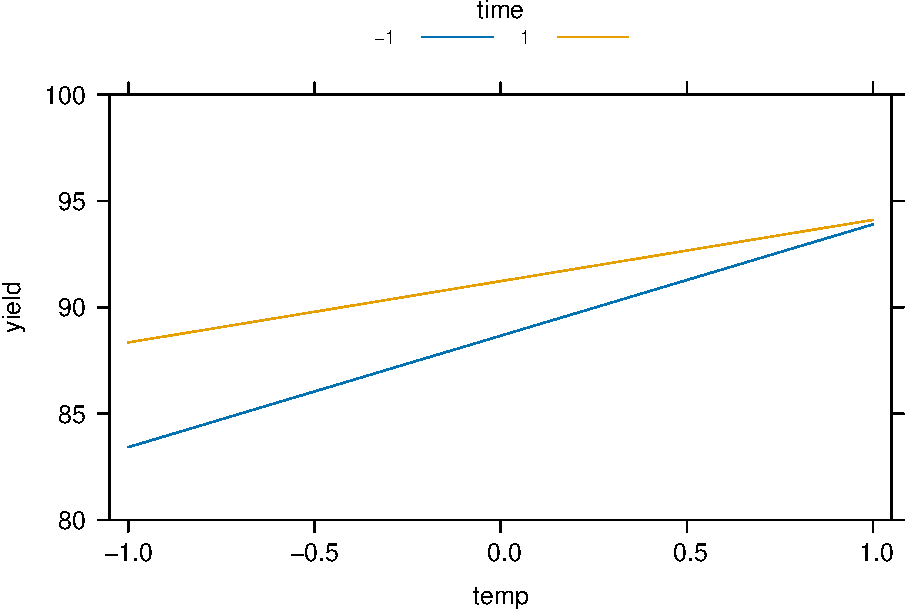
\includegraphics{bookdown_math3014-6027_files/figure-latex/desilylation-effects-1.pdf}
\caption{\label{fig:desilylation-effects}Desilylation experiment: interaction plot generated using the \texttt{effects} package.}
\end{figure}

\hypertarget{anova-for-factorial-experiments}{%
\subsection{ANOVA for factorial experiments}\label{anova-for-factorial-experiments}}

The basic ANOVA table has the following form.

\begin{longtable}[]{@{}
  >{\raggedright\arraybackslash}p{(\columnwidth - 6\tabcolsep) * \real{0.25}}
  >{\raggedright\arraybackslash}p{(\columnwidth - 6\tabcolsep) * \real{0.25}}
  >{\raggedright\arraybackslash}p{(\columnwidth - 6\tabcolsep) * \real{0.25}}
  >{\raggedright\arraybackslash}p{(\columnwidth - 6\tabcolsep) * \real{0.25}}@{}}
\caption{\label{tab:anova-fact} The ANOVA table for a full factorial experiment}\tabularnewline
\toprule
Source & Degress of Freedom & (Sequential) Sum of Squares & Mean Square \\
\midrule
\endfirsthead
\toprule
Source & Degress of Freedom & (Sequential) Sum of Squares & Mean Square \\
\midrule
\endhead
Regression & \(2^f-1\) & \(\sum_{j=1}^{2^f-1}n\hat{\beta}_j^2 - n\bar{y}^2\) & Reg SS/\((2^f-1)\) \\
Residual & \(2^f(r-1)\) & \((\boldsymbol{Y}-X\hat{\boldsymbol{\beta}})^{\textrm{T}}(\boldsymbol{Y}-X\hat{\boldsymbol{\beta}})\) & RSS/\((2^f(r-1))\) \\
Total & \(2^fr-1\) & \(\boldsymbol{Y}^{\textrm{T}}\boldsymbol{Y}-n\bar{Y}^{2}\) & \\
\bottomrule
\end{longtable}

The regression sum of squares for a factorial experiment has a very simple form. If we include an intercept column in \(X\), from Section \ref{anova-revision},

\begin{align*}
\mbox{Regression SS} & = \mbox{RSS(null)} - \mbox{RSS} \\
& = \hat{\boldsymbol{\beta}}^{\mathrm{T}}X^{\mathrm{T}}X\hat{\boldsymbol{\beta}} - n\bar{y}^2 \\
& = \sum_{j=1}^{2^f-1}n\hat{\beta}_j^2 - n\bar{y}^2\,,
\end{align*}

as \(X^{\mathrm{T}}X = nI_{2^f}\). Hence, the \(j\)th factorial effect contributes \(n\hat{\beta}_j^2\) to the regression sum if squares, and this quantity can be used to construct a test statistic \textbf{if} \(r>1\) and hence an estimate of \(\sigma^2\) is available. For Example \ref{exm:factorial-desilylation}, the regression sum of squares and ANOVA table are given in Tables \ref{tab:desilylation-regss} and \ref{tab:desilylation-anova-ss}.

\begin{Shaded}
\begin{Highlighting}[]
\NormalTok{ss }\OtherTok{\textless{}{-}} \FunctionTok{nrow}\NormalTok{(desilylation) }\SpecialCharTok{*} \FunctionTok{coef}\NormalTok{(desilylation\_reg.lm)}\SpecialCharTok{\^{}}\DecValTok{2}
\NormalTok{regss }\OtherTok{\textless{}{-}} \FunctionTok{sum}\NormalTok{(ss) }\SpecialCharTok{{-}} \FunctionTok{nrow}\NormalTok{(desilylation) }\SpecialCharTok{*} \FunctionTok{mean}\NormalTok{(desilylation}\SpecialCharTok{$}\NormalTok{yield)}\SpecialCharTok{\^{}}\DecValTok{2}
\FunctionTok{names}\NormalTok{(regss) }\OtherTok{\textless{}{-}} \StringTok{"Regression"}
\NormalTok{knitr}\SpecialCharTok{::}\FunctionTok{kable}\NormalTok{(}\FunctionTok{c}\NormalTok{(regss, ss[}\SpecialCharTok{{-}}\DecValTok{1}\NormalTok{]), }\AttributeTok{col.names =} \StringTok{"Sum Sq."}\NormalTok{, }\AttributeTok{caption =} \StringTok{"Desilylation experiment: regression sums of squares for each factorial effect calculated directly."}\NormalTok{)}
\end{Highlighting}
\end{Shaded}

\begin{table}

\caption{\label{tab:desilylation-regss}Desilylation experiment: regression sums of squares for each factorial effect calculated directly.}
\centering
\begin{tabular}[t]{l|r}
\hline
  & Sum Sq.\\
\hline
Regression & 427.2837\\
\hline
temp & 263.7376\\
\hline
time & 26.3682\\
\hline
solvent & 19.6692\\
\hline
reagent & 38.1306\\
\hline
temp:time & 22.2312\\
\hline
temp:solvent & 22.2312\\
\hline
temp:reagent & 30.7470\\
\hline
time:solvent & 0.7744\\
\hline
time:reagent & 1.6641\\
\hline
solvent:reagent & 0.9604\\
\hline
temp:time:solvent & 0.2401\\
\hline
temp:time:reagent & 0.1521\\
\hline
temp:solvent:reagent & 0.0036\\
\hline
time:solvent:reagent & 0.2256\\
\hline
temp:time:solvent:reagent & 0.1482\\
\hline
\end{tabular}
\end{table}

\begin{Shaded}
\begin{Highlighting}[]
\NormalTok{knitr}\SpecialCharTok{::}\FunctionTok{kable}\NormalTok{(}\FunctionTok{anova}\NormalTok{(desilylation\_reg.lm)[, }\DecValTok{1}\SpecialCharTok{:}\DecValTok{2}\NormalTok{], }\AttributeTok{caption =} \StringTok{"Desilylation experiment: ANOVA table from \textasciigrave{}anova\textasciigrave{} function."}\NormalTok{)}
\end{Highlighting}
\end{Shaded}

\begin{verbatim}
## Warning in anova.lm(desilylation_reg.lm): ANOVA F-tests on an essentially
## perfect fit are unreliable
\end{verbatim}

\begin{table}

\caption{\label{tab:desilylation-anova-ss}Desilylation experiment: ANOVA table from `anova` function.}
\centering
\begin{tabular}[t]{l|r|r}
\hline
  & Df & Sum Sq\\
\hline
temp & 1 & 263.7376\\
\hline
time & 1 & 26.3682\\
\hline
solvent & 1 & 19.6692\\
\hline
reagent & 1 & 38.1306\\
\hline
temp:time & 1 & 22.2312\\
\hline
temp:solvent & 1 & 22.2312\\
\hline
temp:reagent & 1 & 30.7470\\
\hline
time:solvent & 1 & 0.7744\\
\hline
time:reagent & 1 & 1.6641\\
\hline
solvent:reagent & 1 & 0.9604\\
\hline
temp:time:solvent & 1 & 0.2401\\
\hline
temp:time:reagent & 1 & 0.1521\\
\hline
temp:solvent:reagent & 1 & 0.0036\\
\hline
time:solvent:reagent & 1 & 0.2256\\
\hline
temp:time:solvent:reagent & 1 & 0.1482\\
\hline
Residuals & 0 & 0.0000\\
\hline
\end{tabular}
\end{table}

\hypertarget{exercises-3}{%
\section{Exercises}\label{exercises-3}}

\begin{enumerate}
\def\labelenumi{\arabic{enumi}.}
\item
  A reactor experiment that was presented by Box, Hunter and Hunter (2005, pp259-261) that used a full factorial design for \(m=5\) factors, each at two levels, to investigate the effect of \emph{feed rate} (litres/min), \emph{catalyst} (\%), \emph{agitation rate} (rpm), \emph{temperature} (C) and \emph{concentration} (\%) on the \emph{percentage reacted}. The levels of the experimental factors will be coded as \(-1\) for low level, and \(1\) for high level. Table \ref{tab:reactor-expt} presents the true factor settings corresponding to these coded values.

  \begin{longtable}[]{@{}ccc@{}}
  \caption{\label{tab:reactor-expt} Factor levels for the full factorial reactor experiment}\tabularnewline
  \toprule
  Factor & Low level (\(-1\)) & High level (\(1\)) \\
  \midrule
  \endfirsthead
  \toprule
  Factor & Low level (\(-1\)) & High level (\(1\)) \\
  \midrule
  \endhead
  Feed Rate (litres/min) & 10 & 15 \\
  Catalyst (\%) & 1 & 2 \\
  Agitation Rate (rpm) & 100 & 120 \\
  Temperature (C) & 140 & 180 \\
  Concentration (\%) & 3 & 6 \\
  \bottomrule
  \end{longtable}

  The data from this experiment is given in Table \ref{tab:reactor-data}.

\begin{Shaded}
\begin{Highlighting}[]
\NormalTok{reactor.frf2 }\OtherTok{\textless{}{-}}\NormalTok{ FrF2}\SpecialCharTok{::}\FunctionTok{FrF2}\NormalTok{(}\AttributeTok{nruns =} \DecValTok{32}\NormalTok{, }\AttributeTok{nfactors =} \DecValTok{5}\NormalTok{, }\AttributeTok{randomize =}\NormalTok{ F,}
                           \AttributeTok{factor.names =} \FunctionTok{c}\NormalTok{(}\StringTok{"FR"}\NormalTok{, }\StringTok{"Cat"}\NormalTok{, }\StringTok{"AR"}\NormalTok{, }\StringTok{"Temp"}\NormalTok{, }\StringTok{"Conc"}\NormalTok{))}
\NormalTok{y }\OtherTok{\textless{}{-}} \FunctionTok{c}\NormalTok{(}\DecValTok{61}\NormalTok{, }\DecValTok{53}\NormalTok{, }\DecValTok{63}\NormalTok{, }\DecValTok{61}\NormalTok{, }\DecValTok{53}\NormalTok{, }\DecValTok{56}\NormalTok{, }\DecValTok{54}\NormalTok{, }\DecValTok{61}\NormalTok{, }\DecValTok{69}\NormalTok{, }\DecValTok{61}\NormalTok{, }\DecValTok{94}\NormalTok{, }\DecValTok{93}\NormalTok{, }\DecValTok{66}\NormalTok{, }\DecValTok{60}\NormalTok{, }\DecValTok{95}\NormalTok{, }\DecValTok{98}\NormalTok{, }\DecValTok{56}\NormalTok{, }\DecValTok{63}\NormalTok{,}
       \DecValTok{70}\NormalTok{, }\DecValTok{65}\NormalTok{, }\DecValTok{59}\NormalTok{, }\DecValTok{55}\NormalTok{, }\DecValTok{67}\NormalTok{, }\DecValTok{65}\NormalTok{, }\DecValTok{44}\NormalTok{, }\DecValTok{45}\NormalTok{, }\DecValTok{78}\NormalTok{, }\DecValTok{77}\NormalTok{, }\DecValTok{49}\NormalTok{, }\DecValTok{42}\NormalTok{, }\DecValTok{81}\NormalTok{, }\DecValTok{82}\NormalTok{)}
\NormalTok{reactor }\OtherTok{\textless{}{-}} \FunctionTok{data.frame}\NormalTok{(reactor.frf2, }\AttributeTok{pre.react =}\NormalTok{ y)}
\NormalTok{knitr}\SpecialCharTok{::}\FunctionTok{kable}\NormalTok{(reactor, }\AttributeTok{caption =} \StringTok{"Reactor experiment."}\NormalTok{)}
\end{Highlighting}
\end{Shaded}

  \begin{table}

   \caption{\label{tab:reactor-data}Reactor experiment.}
   \centering
   \begin{tabular}[t]{l|l|l|l|l|r}
   \hline
   FR & Cat & AR & Temp & Conc & pre.react\\
   \hline
   -1 & -1 & -1 & -1 & -1 & 61\\
   \hline
   1 & -1 & -1 & -1 & -1 & 53\\
   \hline
   -1 & 1 & -1 & -1 & -1 & 63\\
   \hline
   1 & 1 & -1 & -1 & -1 & 61\\
   \hline
   -1 & -1 & 1 & -1 & -1 & 53\\
   \hline
   1 & -1 & 1 & -1 & -1 & 56\\
   \hline
   -1 & 1 & 1 & -1 & -1 & 54\\
   \hline
   1 & 1 & 1 & -1 & -1 & 61\\
   \hline
   -1 & -1 & -1 & 1 & -1 & 69\\
   \hline
   1 & -1 & -1 & 1 & -1 & 61\\
   \hline
   -1 & 1 & -1 & 1 & -1 & 94\\
   \hline
   1 & 1 & -1 & 1 & -1 & 93\\
   \hline
   -1 & -1 & 1 & 1 & -1 & 66\\
   \hline
   1 & -1 & 1 & 1 & -1 & 60\\
   \hline
   -1 & 1 & 1 & 1 & -1 & 95\\
   \hline
   1 & 1 & 1 & 1 & -1 & 98\\
   \hline
   -1 & -1 & -1 & -1 & 1 & 56\\
   \hline
   1 & -1 & -1 & -1 & 1 & 63\\
   \hline
   -1 & 1 & -1 & -1 & 1 & 70\\
   \hline
   1 & 1 & -1 & -1 & 1 & 65\\
   \hline
   -1 & -1 & 1 & -1 & 1 & 59\\
   \hline
   1 & -1 & 1 & -1 & 1 & 55\\
   \hline
   -1 & 1 & 1 & -1 & 1 & 67\\
   \hline
   1 & 1 & 1 & -1 & 1 & 65\\
   \hline
   -1 & -1 & -1 & 1 & 1 & 44\\
   \hline
   1 & -1 & -1 & 1 & 1 & 45\\
   \hline
   -1 & 1 & -1 & 1 & 1 & 78\\
   \hline
   1 & 1 & -1 & 1 & 1 & 77\\
   \hline
   -1 & -1 & 1 & 1 & 1 & 49\\
   \hline
   1 & -1 & 1 & 1 & 1 & 42\\
   \hline
   -1 & 1 & 1 & 1 & 1 & 81\\
   \hline
   1 & 1 & 1 & 1 & 1 & 82\\
   \hline
   \end{tabular}
   \end{table}

  \begin{enumerate}
  \def\labelenumii{\alph{enumii}.}
  \item
    Estimate all the factorial effects from this experiment, and use a half-normal plot and Lenth's method to decide which are significantly different from zero.
  \item
    Use the \texttt{effects} package to produce main effect and/or interaction plots for each significant factorial effect from part a.
  \item
    Now fit a regression model that only includes terms corresponding to main effects and two-factor interactions. How many degrees of freedom does this model use? What does this mean for the estimation of \(\sigma^2\)? How does the estimate of \(\sigma^2\) from this model relate to your analysis in part a?
  \end{enumerate}
\end{enumerate}

Solution

\begin{enumerate}
\def\labelenumi{\alph{enumi}.}
\tightlist
\item
  We will estimate the factorial effects as twice the corresponding regression parameters.
\end{enumerate}

\begin{Shaded}
\begin{Highlighting}[]
\NormalTok{reactor }\OtherTok{\textless{}{-}}\NormalTok{ dplyr}\SpecialCharTok{::}\FunctionTok{mutate}\NormalTok{(reactor, }\FunctionTok{across}\NormalTok{(}\AttributeTok{.cols =}\NormalTok{ FR}\SpecialCharTok{:}\NormalTok{Conc, }
                                         \SpecialCharTok{\textasciitilde{}} \FunctionTok{as.numeric}\NormalTok{(}\FunctionTok{as.character}\NormalTok{(.x))))}
\NormalTok{reactor.lm }\OtherTok{\textless{}{-}} \FunctionTok{lm}\NormalTok{(pre.react }\SpecialCharTok{\textasciitilde{}}\NormalTok{ (.) }\SpecialCharTok{\^{}} \DecValTok{5}\NormalTok{, }\AttributeTok{data =}\NormalTok{ reactor)}
\NormalTok{fac.effects }\OtherTok{\textless{}{-}} \DecValTok{2} \SpecialCharTok{*} \FunctionTok{coef}\NormalTok{(reactor.lm)[}\SpecialCharTok{{-}}\DecValTok{1}\NormalTok{]}
\NormalTok{knitr}\SpecialCharTok{::}\FunctionTok{kable}\NormalTok{(fac.effects, }\AttributeTok{caption =} \StringTok{"Reactor experiment: estimated factorial effects."}\NormalTok{)}
\end{Highlighting}
\end{Shaded}

\begin{table}

\caption{\label{tab:reactor-estimate}Reactor experiment: estimated factorial effects.}
\centering
\begin{tabular}[t]{l|r}
\hline
  & x\\
\hline
FR & -1.375\\
\hline
Cat & 19.500\\
\hline
AR & -0.625\\
\hline
Temp & 10.750\\
\hline
Conc & -6.250\\
\hline
FR:Cat & 1.375\\
\hline
FR:AR & 0.750\\
\hline
FR:Temp & -0.875\\
\hline
FR:Conc & 0.125\\
\hline
Cat:AR & 0.875\\
\hline
Cat:Temp & 13.250\\
\hline
Cat:Conc & 2.000\\
\hline
AR:Temp & 2.125\\
\hline
AR:Conc & 0.875\\
\hline
Temp:Conc & -11.000\\
\hline
FR:Cat:AR & 1.500\\
\hline
FR:Cat:Temp & 1.375\\
\hline
FR:Cat:Conc & -1.875\\
\hline
FR:AR:Temp & -0.750\\
\hline
FR:AR:Conc & -2.500\\
\hline
FR:Temp:Conc & 0.625\\
\hline
Cat:AR:Temp & 1.125\\
\hline
Cat:AR:Conc & 0.125\\
\hline
Cat:Temp:Conc & -0.250\\
\hline
AR:Temp:Conc & 0.125\\
\hline
FR:Cat:AR:Temp & 0.000\\
\hline
FR:Cat:AR:Conc & 1.500\\
\hline
FR:Cat:Temp:Conc & 0.625\\
\hline
FR:AR:Temp:Conc & 1.000\\
\hline
Cat:AR:Temp:Conc & -0.625\\
\hline
FR:Cat:AR:Temp:Conc & -0.500\\
\hline
\end{tabular}
\end{table}

There are several large factorial effects, including the main effects of Catalyst and Temperature and the interaction between these factors, and the interaction between Concentration and Temperature. We can assess their significance using a half-normal plot and Lenth's method.

\begin{Shaded}
\begin{Highlighting}[]
\NormalTok{unrepx}\SpecialCharTok{::}\FunctionTok{hnplot}\NormalTok{(fac.effects, }\AttributeTok{horiz =}\NormalTok{ F, }\AttributeTok{method =} \StringTok{"Lenth"}\NormalTok{, }\AttributeTok{alpha =} \FloatTok{0.05}\NormalTok{)}
\end{Highlighting}
\end{Shaded}

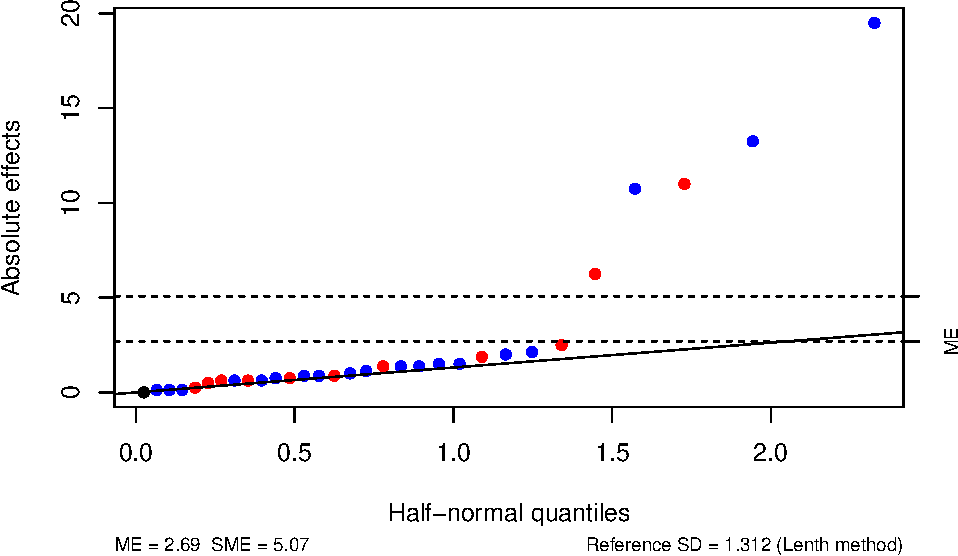
\includegraphics{bookdown_math3014-6027_files/figure-latex/reactor-lenth-1.pdf}

We see that PSE = 1.3125, giving individual and simultaneous margins of error of 2.6892 and 5.1375, respectively (where the latter is adjusted for multiple testing). There is a very clear distinction between the five effects which are largest in absolute value and the other factorial effects, which form a very clear line. The five of the largest effects are given in Table \ref{tab:reactor-largest}, are all greater than both margins of error and can be declared as significant.

\begin{Shaded}
\begin{Highlighting}[]
\NormalTok{knitr}\SpecialCharTok{::}\FunctionTok{kable}\NormalTok{(fac.effects[}\FunctionTok{abs}\NormalTok{(fac.effects) }\SpecialCharTok{\textgreater{}}\NormalTok{ unrepx}\SpecialCharTok{::}\FunctionTok{ME}\NormalTok{(fac.effects, }
                                                       \AttributeTok{method =} \StringTok{"Lenth"}\NormalTok{)[}\DecValTok{2}\NormalTok{]],}
             \AttributeTok{caption =} \StringTok{"Reactor experiment: factorial effects significantly different from zero via Lenth\textquotesingle{}s method."}\NormalTok{)}
\end{Highlighting}
\end{Shaded}

\begin{table}

\caption{\label{tab:reactor-largest}Reactor experiment: factorial effects significantly different from zero via Lenth's method.}
\centering
\begin{tabular}[t]{l|r}
\hline
  & x\\
\hline
Cat & 19.50\\
\hline
Temp & 10.75\\
\hline
Conc & -6.25\\
\hline
Cat:Temp & 13.25\\
\hline
Temp:Conc & -11.00\\
\hline
\end{tabular}
\end{table}

\begin{enumerate}
\def\labelenumi{\alph{enumi}.}
\setcounter{enumi}{1}
\tightlist
\item
  We will produce plots for the interactions between Catalyst and Temperature and Temperature and Concentration. We will not produce main effect plots for Catalyst and Temperature, as these are involved in the large interactions.
\end{enumerate}

\begin{Shaded}
\begin{Highlighting}[]
\NormalTok{Cat\_x\_Temp }\OtherTok{\textless{}{-}}\NormalTok{ effects}\SpecialCharTok{::}\FunctionTok{Effect}\NormalTok{(}\FunctionTok{c}\NormalTok{(}\StringTok{"Cat"}\NormalTok{, }\StringTok{"Temp"}\NormalTok{), reactor.lm, }
                              \AttributeTok{xlevels =} \FunctionTok{list}\NormalTok{(}\AttributeTok{Cat =} \FunctionTok{c}\NormalTok{(}\SpecialCharTok{{-}}\DecValTok{1}\NormalTok{, }\DecValTok{1}\NormalTok{), }\AttributeTok{Temp =} \FunctionTok{c}\NormalTok{(}\SpecialCharTok{{-}}\DecValTok{1}\NormalTok{, }\DecValTok{1}\NormalTok{)), }
                              \AttributeTok{se =}\NormalTok{ F)}
\NormalTok{Temp\_x\_Conc }\OtherTok{\textless{}{-}}\NormalTok{ effects}\SpecialCharTok{::}\FunctionTok{Effect}\NormalTok{(}\FunctionTok{c}\NormalTok{(}\StringTok{"Temp"}\NormalTok{, }\StringTok{"Conc"}\NormalTok{), reactor.lm, }
                               \AttributeTok{xlevels =} \FunctionTok{list}\NormalTok{(}\AttributeTok{Conc =} \FunctionTok{c}\NormalTok{(}\SpecialCharTok{{-}}\DecValTok{1}\NormalTok{, }\DecValTok{1}\NormalTok{), }\AttributeTok{Temp =} \FunctionTok{c}\NormalTok{(}\SpecialCharTok{{-}}\DecValTok{1}\NormalTok{, }\DecValTok{1}\NormalTok{)),}
                               \AttributeTok{se =}\NormalTok{ F)}
\FunctionTok{plot}\NormalTok{(Cat\_x\_Temp, }\AttributeTok{style =} \StringTok{"stacked"}\NormalTok{, }\AttributeTok{main =} \StringTok{""}\NormalTok{, }\AttributeTok{rug =}\NormalTok{ F, }\AttributeTok{x.var =} \StringTok{"Cat"}\NormalTok{, }
     \AttributeTok{ylim =} \FunctionTok{c}\NormalTok{(}\DecValTok{50}\NormalTok{, }\DecValTok{90}\NormalTok{))}
\FunctionTok{plot}\NormalTok{(Temp\_x\_Conc, }\AttributeTok{style =} \StringTok{"stacked"}\NormalTok{, }\AttributeTok{main =} \StringTok{""}\NormalTok{, }\AttributeTok{rug =}\NormalTok{ F, }\AttributeTok{x.var =} \StringTok{"Conc"}\NormalTok{, }
     \AttributeTok{ylim =} \FunctionTok{c}\NormalTok{(}\DecValTok{50}\NormalTok{, }\DecValTok{90}\NormalTok{))}
\end{Highlighting}
\end{Shaded}

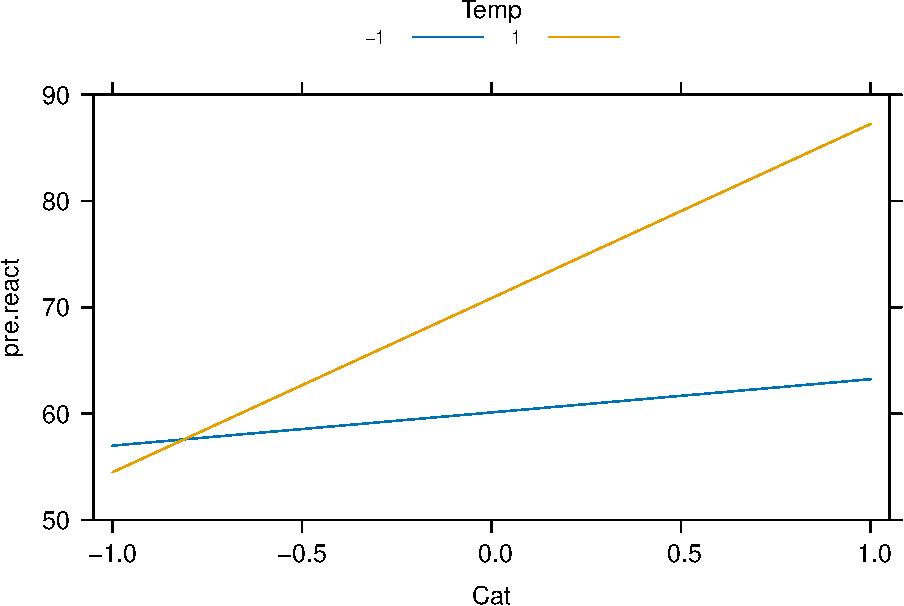
\includegraphics{bookdown_math3014-6027_files/figure-latex/reactor-plots-1.pdf} 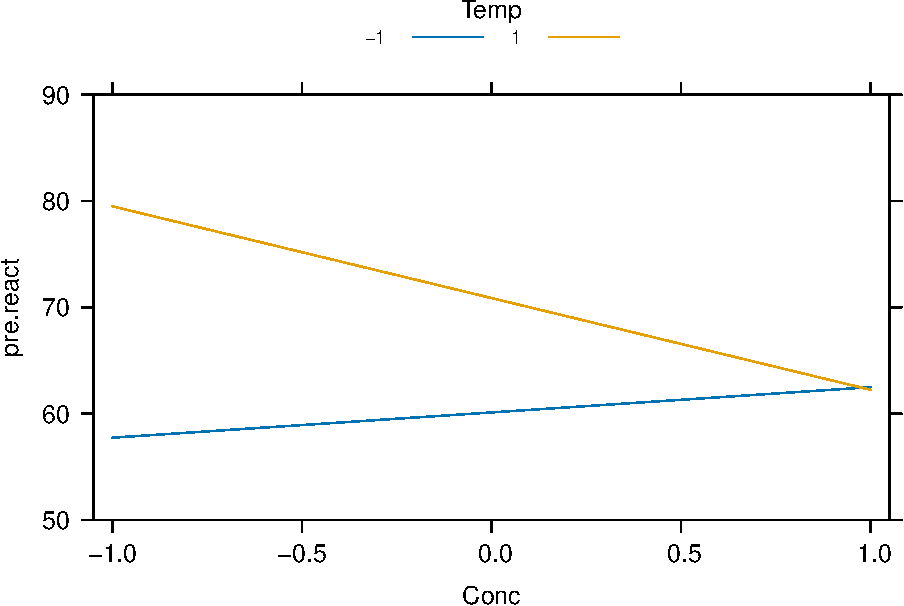
\includegraphics{bookdown_math3014-6027_files/figure-latex/reactor-plots-2.pdf}
Notice that changing the level of Temperature changes substantial the effect of both Catalyst and Concentration on the response; in particular, the effect of Concentration changes sign depending on the level of Temperature.

\begin{enumerate}
\def\labelenumi{\alph{enumi}.}
\setcounter{enumi}{2}
\tightlist
\item
  We start by fiting the reduced regression model.
\end{enumerate}

\begin{Shaded}
\begin{Highlighting}[]
\NormalTok{reactor2.lm }\OtherTok{\textless{}{-}} \FunctionTok{lm}\NormalTok{(pre.react }\SpecialCharTok{\textasciitilde{}}\NormalTok{ (.) }\SpecialCharTok{\^{}} \DecValTok{2}\NormalTok{, }\AttributeTok{data =}\NormalTok{ reactor)}
\FunctionTok{summary}\NormalTok{(reactor2.lm)}
\end{Highlighting}
\end{Shaded}

\begin{verbatim}
## 
## Call:
## lm(formula = pre.react ~ (.)^2, data = reactor)
## 
## Residuals:
##    Min     1Q Median     3Q    Max 
##  -5.00  -1.62  -0.25   1.75   4.50 
## 
## Coefficients:
##             Estimate Std. Error t value        Pr(>|t|)    
## (Intercept)  65.5000     0.5660  115.73         < 2e-16 ***
## FR           -0.6875     0.5660   -1.21           0.242    
## Cat           9.7500     0.5660   17.23 0.0000000000094 ***
## AR           -0.3125     0.5660   -0.55           0.588    
## Temp          5.3750     0.5660    9.50 0.0000000560392 ***
## Conc         -3.1250     0.5660   -5.52 0.0000464538196 ***
## FR:Cat        0.6875     0.5660    1.21           0.242    
## FR:AR         0.3750     0.5660    0.66           0.517    
## FR:Temp      -0.4375     0.5660   -0.77           0.451    
## FR:Conc       0.0625     0.5660    0.11           0.913    
## Cat:AR        0.4375     0.5660    0.77           0.451    
## Cat:Temp      6.6250     0.5660   11.71 0.0000000029456 ***
## Cat:Conc      1.0000     0.5660    1.77           0.096 .  
## AR:Temp       1.0625     0.5660    1.88           0.079 .  
## AR:Conc       0.4375     0.5660    0.77           0.451    
## Temp:Conc    -5.5000     0.5660   -9.72 0.0000000408373 ***
## ---
## Signif. codes:  0 '***' 0.001 '**' 0.01 '*' 0.05 '.' 0.1 ' ' 1
## 
## Residual standard error: 3.2 on 16 degrees of freedom
## Multiple R-squared:  0.976,  Adjusted R-squared:  0.954 
## F-statistic: 44.1 on 15 and 16 DF,  p-value: 0.000000000376
\end{verbatim}

This model includes regression parameters corresponding to \(5 + {5 \choose 2} = 15\) factorial effects, plus the intercept, and hence uses 16 degrees of freedom. The remaining 16 degrees of freedom, which were previously used to estimate three-factor and higher interactions, is now used to estimate \(\sigma^2\), the background variation.

The residual mean square in the reduced model, used to estimate \(\sigma^2\), is the sum of the sums of squares for the higher-order interactions in the original model, divided by 16 (the remaining degrees of freedom).

\begin{Shaded}
\begin{Highlighting}[]
\FunctionTok{sum}\NormalTok{(}\FunctionTok{anova}\NormalTok{(reactor.lm)[}\DecValTok{16}\SpecialCharTok{:}\DecValTok{31}\NormalTok{, }\DecValTok{3}\NormalTok{]) }\SpecialCharTok{/} \DecValTok{16}
\end{Highlighting}
\end{Shaded}

\begin{verbatim}
## [1] 10.25
\end{verbatim}

\begin{Shaded}
\begin{Highlighting}[]
\FunctionTok{summary}\NormalTok{(reactor2.lm)}\SpecialCharTok{$}\NormalTok{sigma}\SpecialCharTok{\^{}}\DecValTok{2}
\end{Highlighting}
\end{Shaded}

\begin{verbatim}
## [1] 10.25
\end{verbatim}

This ``pooling'' of higher-order effects to estimate \(\sigma^2\) maybe a reasonable strategy here, given that the high-order interactions are all small, but could be biased if one or more interactions were large.

\begin{enumerate}
\def\labelenumi{\arabic{enumi}.}
\setcounter{enumi}{1}
\item
  \citep[Adapted from][]{Morris2011} Consider an unreplicated (\(r=1\)) \(2^6\) factorial experiment. The total sums of squares,

  \[
  \mbox{Total SS} = \sum_{i=1}^n(y_i - \bar{y})^2\,,
  \]

  has value 2856. Using Lenth's method, an informal analysis of the data suggests that there are only three important factorial effects, with least squares estimates

  \begin{itemize}
  \tightlist
  \item
    main effect of factor \(A\) = 3
  \item
    interaction between factors \(A\) and \(B\) = 4
  \item
    interaction between factors \(A\), \(B\) and \(C\) = 2.
  \end{itemize}

  If a linear model including only an intercept and these three effects is fitted to the data, what is the value of the residual sum of squares?
\end{enumerate}

Solution

The residual sum of squares has the form

\[
\mbox{RSS} = (\boldsymbol{y}- X\hat
{\boldsymbol{\beta}})^{\mathrm{T}}(\boldsymbol{y}- X\hat
{\boldsymbol{\beta}})\,,  
\]

where in this case \(X\) is a \(2^6\times 4\) model matrix, with columsn corresponding to the intercept, main effect of factor \(A\), the interaction between factors \(A\) and \(B\), the interaction between factors \(A\), \(B\) and \(C\). We can rewrite the RSS as

\begin{equation*}
\begin{split}
\mbox{RSS} & = (\boldsymbol{y}- X\hat
{\boldsymbol{\beta}})^{\mathrm{T}}(\boldsymbol{y}- X\hat
{\boldsymbol{\beta}}) \\
& = \boldsymbol{y}^{\mathrm{T}}\boldsymbol{y}- 2\boldsymbol{y}^{\mathrm{T}}X\hat
{\boldsymbol{\beta}} + \hat
{\boldsymbol{\beta}}^{\mathrm{T}}X^{\mathrm{T}}X\hat
{\boldsymbol{\beta}} \\
& = \boldsymbol{y}^{\mathrm{T}}\boldsymbol{y}- 2\hat
{\boldsymbol{\beta}}^{\mathrm{T}}X^{\mathrm{T}}X\hat
{\boldsymbol{\beta}} + \hat
{\boldsymbol{\beta}}^{\mathrm{T}}X^{\mathrm{T}}X\hat
{\boldsymbol{\beta}} \\
& = \boldsymbol{y}^{\mathrm{T}}\boldsymbol{y}- \hat
{\boldsymbol{\beta}}^{\mathrm{T}}X^{\mathrm{T}}X\hat
{\boldsymbol{\beta}}\,, 
\end{split}
\end{equation*}

as \(\boldsymbol{y}^{\mathrm{T}}X = \hat{\boldsymbol{\beta}}^{\mathrm{T}}X^{\mathrm{T}}X\).

Due the matrix \(X\) having orthogonal columns, \(X^{\mathrm{T}}X = 2^fI_{p+1}\), for a model containing coefficients corresponding to \(p\) factorial effects; here, \(p=3\). Hence,

\[
\mbox{RSS} = \boldsymbol{y}^{\mathrm{T}}\boldsymbol{y}- 2^f \sum_{i=0}^{p}\hat{\beta}_i^2\,.
\]

Finally, the estimate of the intercept takes the form \(\hat{\beta}_0 = \bar{Y}\), and so

\begin{equation*}
\begin{split}
\mbox{RSS} & = \boldsymbol{y}^{\mathrm{T}}\boldsymbol{y}- 2^f\bar{y} -  2^f\sum_{i=1}^{p}\hat{\beta}_i^2 \\
& = \sum_{i=1}^{2^f}(y_i - \bar{y})^2 - 2^f\sum_{i=1}^{p}\hat{\beta}_i^2 \\
& = \mbox{Total SS} - 2^f\sum_{i=1}^{p}\hat{\beta}_i^2\,
\end{split}
\end{equation*}

Recalling that each regression coefficient is one-half of the corresponding factorial effect, for this example we have:

\[
\mbox{RSS} = 2856 - 2^6(1.5^2 + 2^2 + 1^2) = 2392\,.
\]

\begin{enumerate}
\def\labelenumi{\arabic{enumi}.}
\setcounter{enumi}{2}
\item
  \citep[Adapted from][]{Morris2011} Consider a \(2^7\) experiment with each treatment applied to two units (\(r=2\)). Assume a linear regression model will be fitted containing terms corresponding to all factorial effects.

  \begin{enumerate}
  \def\labelenumii{\alph{enumii}.}
  \item
    What is the variance of the estimator of each factorial effect, up to a constant factor \(\sigma^2\)?
  \item
    What is the variance of the least squares estimator of \(E(y_{11})\), the expected value of an observation with the first treatment applied? You can assume the treatments are given in standard order, so the first treatment is defined by setting all factors to their low level. {[}The answer is, obviously, the same for \(E(y_{12})\){]}. In a practical experimental setting, why is this not a useful quantity to estimate?
  \item
    What is the variance of the least squares estimator of \(E(y_{11}) - E(y_{21})\)? You may assume that the second treatment has all factors set to their low levels except for the seventh factor.
  \end{enumerate}
\end{enumerate}

Solutions

\begin{enumerate}
\def\labelenumi{\alph{enumi}.}
\item
  Each factorial contrast is scaled so the variance for the estimator is equal to \(4\sigma^2/n = \sigma^2 / 64\).
\item
  \(E(y_11) = \boldsymbol{x}_1^{\mathrm{T}}\boldsymbol{\beta}\), where \(\boldsymbol{x}_1^{\mathrm{T}}\) is the row of the \(X\) matrix corresponding to the first treatment and \(\boldsymbol{\beta}\) are the regression coefficients. The estimator is given by

  \[
  \hat{E}(y_{11}) = \boldsymbol{x}_1^{\mathrm{T}}\hat{\boldsymbol{\beta}}\,,
  \]

  with variance

  \begin{align*}
  \mathrm{var}\left\{\hat{E}(y_{11})\right\} & = \mathrm{var}\left\{\boldsymbol{x}_1^{\mathrm{T}}\hat{\boldsymbol{\beta}}\right\} \\
  & = \boldsymbol{x}_1^{\mathrm{T}}\mbox{var}(\hat{\boldsymbol{\beta}})\boldsymbol{x}_1 \\
  & = \boldsymbol{x}_1^{\mathrm{T}}\left(X^\mathrm{T}X\right)^{-1}\boldsymbol{x}_1\sigma^2 \\
  & = \frac{\boldsymbol{x}_1^{\mathrm{T}}\boldsymbol{x}_1\sigma^2}{2^8} \\
  & = \frac{2^7\sigma^2}{2^8} \\
  & = \sigma^2 / 2\,.
  \end{align*}

  This holds for the expected response from any treatment, as \(\boldsymbol{x}_j^{\mathrm{T}}\boldsymbol{x}_j = 2^7\) for all treatments, as each entry of \(\boldsymbol{x}_j\) is equal to \(\pm 1\).

  This would not be a useful quantity to estimate in a practical experiment, as it is not a contrast in the treatments. In particular, it depends on the estimate of the overall mean, \(\mu\) or \(\beta_0\) (in the unit-treatment or regression model) that will vary from experiment to experiment.
\item
  The expected values of \(y_{11}\) and \(y_{21}\) will only differ in terms involving the seventh factor, which is equal to its low level (-1) for the first treatment and its high level (+1) for the second treatment; all the other terms will cancel. Hence

  \[
  E(y_{11}) - E(y_{21}) = -2\left(\beta_7 + \sum_{j=1}^6\beta_{j7} + \sum_{j=1}^6\sum_{k=j+1}^6\beta_{jk7} + \ldots + \beta_{1234567}\right)\,.
  \]

  The variance of the estimator has the form

  \begin{align*}
  \mathrm{var}\left\{\widehat{E(y_{11}) - E(y_{21})}\right\} & = 4\times\mathrm{var}\bigg(\hat{\beta}_7 + \sum_{j=1}^6\hat{\beta}_{j7} + \sum_{j=1}^6\sum_{k=j+1}^6\hat{\beta}_{jk7} + \\
  & \ldots + \hat{\beta}_{1234567}\bigg) \\
  & = \frac{4\sigma^2}{2\times 2^7}\sum_{j=0}^6{6 \choose j} \\
  & = \frac{\sigma^2}{2^6}\times 64 \\
  & = \sigma^2\,.
  \end{align*}

  Or, as this is a treatment comparison in a CRD, we have

  \[
   \hat{E}(y_{11}) - \hat{E}(y_{21}) = \widehat{\boldsymbol{c}^{\mathrm{T}}\boldsymbol{\tau}}\,,
  \]

  where \(\boldsymbol{c}\) corresponds to a pairwise treatment comparison, and hence has one entry equal to +1 and one entry equal to -1. From Section \ref{contrast-crd},

  \begin{align*}
  \mathrm{var}\left(\widehat{\boldsymbol{c}^{\mathrm{T}}\boldsymbol{\tau}}\right) 
  & = \sum_{i=1}^tc_i^2\mathrm{var}(\bar{y}_{i.}) \\
  & = \sigma^2\sum_{i=1}^tc_i^2/n_i\,,
  \end{align*}

  where in this example \(n_i = 2\) for all \(i\) and \(\sum_{i=1}^tc_i^2 = 2\). Hence, the variance is again equal to \(\sigma^2\).
\end{enumerate}

\hypertarget{block-factorial}{%
\chapter{Blocking in factorial designs}\label{block-factorial}}

We now consider splitting the treatments in a factorial design into blocks. As in Chapter \ref{blocking}, the simplest factorial blocked design is a \textbf{randomised complete block design}, where the blocks are large enough for a complete replicate of the factorial treatments to occur in each block. Analysis then proceeds as in Chapter \ref{blocking}, with the contrasts of interest being those corresponding to the factorial effects (main effects and interactions).

However, the number of treatments grows rapidly in a factorial design, and it is unusual for the block sizes to be sufficiently large to accomodate a complete replication within each block. Hence, \textbf{incomplete block designs} must be employed. While balanced incomplete block designs (Section \ref{sec-bibd}) can be used, they do not tend to have good statistical properties and their construction is complicated. In this chapter, we will focus on a class of methods specific to splitting a two-level factorial design in to blocks who common size \(k\) is a power of two.

\hypertarget{two-examples}{%
\section{Two examples}\label{two-examples}}

We will use two simple examples to illustrate this approach, based on a \(2^3\) experiment with factors labelled \(A\), \(B\) and \(C\) (Table \ref{tab:example-factorial}).

\begin{Shaded}
\begin{Highlighting}[]
\NormalTok{example.design }\OtherTok{\textless{}{-}}\NormalTok{ FrF2}\SpecialCharTok{::}\FunctionTok{FrF2}\NormalTok{(}\AttributeTok{nruns =} \DecValTok{8}\NormalTok{, }\AttributeTok{nfactors =} \DecValTok{3}\NormalTok{, }\AttributeTok{randomize =}\NormalTok{ F)}
\NormalTok{knitr}\SpecialCharTok{::}\FunctionTok{kable}\NormalTok{(example.design, }\AttributeTok{caption =} \StringTok{"Treatments from a $2\^{}3$ factorial design"}\NormalTok{, }\AttributeTok{align =} \FunctionTok{rep}\NormalTok{(}\StringTok{"r"}\NormalTok{, }\DecValTok{3}\NormalTok{))}
\end{Highlighting}
\end{Shaded}

\begin{table}

\caption{\label{tab:example-factorial}Treatments from a $2^3$ factorial design}
\centering
\begin{tabular}[t]{r|r|r}
\hline
A & B & C\\
\hline
-1 & -1 & -1\\
\hline
1 & -1 & -1\\
\hline
-1 & 1 & -1\\
\hline
1 & 1 & -1\\
\hline
-1 & -1 & 1\\
\hline
1 & -1 & 1\\
\hline
-1 & 1 & 1\\
\hline
1 & 1 & 1\\
\hline
\end{tabular}
\end{table}

\begin{example}
\protect\hypertarget{exm:block-frac-1}{}\label{exm:block-frac-1}

Consider splitting the treatments between two blocks of size \(2^{3-1}=4\). One choice is given in Table \ref{tab:block-frac-1}.

\begin{Shaded}
\begin{Highlighting}[]
\NormalTok{block1 }\OtherTok{\textless{}{-}} \FunctionTok{c}\NormalTok{(}\DecValTok{1}\NormalTok{, }\DecValTok{2}\NormalTok{, }\DecValTok{2}\NormalTok{, }\DecValTok{1}\NormalTok{, }\DecValTok{2}\NormalTok{, }\DecValTok{1}\NormalTok{, }\DecValTok{1}\NormalTok{, }\DecValTok{2}\NormalTok{)}
\NormalTok{example.design.a }\OtherTok{\textless{}{-}} \FunctionTok{cbind}\NormalTok{(example.design, }\AttributeTok{Block =}\NormalTok{ block1)}
\NormalTok{knitr}\SpecialCharTok{::}\FunctionTok{kable}\NormalTok{(example.design.a, }\AttributeTok{caption =} \StringTok{"Treatments from a $2\^{}3$ factorial design split into two blocks of size four."}\NormalTok{, }\AttributeTok{align =} \FunctionTok{rep}\NormalTok{(}\StringTok{"r"}\NormalTok{, }\DecValTok{4}\NormalTok{))}
\end{Highlighting}
\end{Shaded}

\begin{table}

\caption{\label{tab:block-frac-1}Treatments from a $2^3$ factorial design split into two blocks of size four.}
\centering
\begin{tabular}[t]{r|r|r|r}
\hline
A & B & C & Block\\
\hline
-1 & -1 & -1 & 1\\
\hline
1 & -1 & -1 & 2\\
\hline
-1 & 1 & -1 & 2\\
\hline
1 & 1 & -1 & 1\\
\hline
-1 & -1 & 1 & 2\\
\hline
1 & -1 & 1 & 1\\
\hline
-1 & 1 & 1 & 1\\
\hline
1 & 1 & 1 & 2\\
\hline
\end{tabular}
\end{table}

To assess the impact of this choice of blocking scheme on the analysis of the experiment, we need to consider the (unscaled) contrasts corresponding to all the factorial effects, see Table \ref{tab:block-frac-1-mm}.

\begin{Shaded}
\begin{Highlighting}[]
\NormalTok{X }\OtherTok{\textless{}{-}} \FunctionTok{model.matrix}\NormalTok{( }\SpecialCharTok{\textasciitilde{}}\NormalTok{ Block }\SpecialCharTok{+}\NormalTok{ (A }\SpecialCharTok{+}\NormalTok{ B }\SpecialCharTok{+}\NormalTok{ C)}\SpecialCharTok{\^{}}\DecValTok{3}\NormalTok{, }\AttributeTok{data =}\NormalTok{ example.design.a)}
\NormalTok{Xdf }\OtherTok{\textless{}{-}} \FunctionTok{data.frame}\NormalTok{(X[, }\SpecialCharTok{{-}}\DecValTok{1}\NormalTok{])}
\FunctionTok{colnames}\NormalTok{(Xdf) }\OtherTok{\textless{}{-}} \FunctionTok{c}\NormalTok{(}\StringTok{"Block"}\NormalTok{, }\StringTok{"A"}\NormalTok{, }\StringTok{"B"}\NormalTok{, }\StringTok{"C"}\NormalTok{, }\StringTok{"A:B"}\NormalTok{, }\StringTok{"A:C"}\NormalTok{, }\StringTok{"B:C"}\NormalTok{, }\StringTok{"A:B:C"}\NormalTok{)}
\NormalTok{Xdf }\OtherTok{\textless{}{-}}\NormalTok{ dplyr}\SpecialCharTok{::}\FunctionTok{mutate}\NormalTok{(Xdf, }\AttributeTok{Treatment =} \DecValTok{1}\SpecialCharTok{:}\DecValTok{8}\NormalTok{, }\AttributeTok{.before =}\NormalTok{ Block)}
\NormalTok{knitr}\SpecialCharTok{::}\FunctionTok{kable}\NormalTok{(Xdf, }\AttributeTok{caption =} \StringTok{"Unscaled factorial effect contrasts for a $2\^{}3$ design with one possible assignment of treatments to blocks"}\NormalTok{)}
\end{Highlighting}
\end{Shaded}

\begin{table}

\caption{\label{tab:block-frac-1-mm}Unscaled factorial effect contrasts for a $2^3$ design with one possible assignment of treatments to blocks}
\centering
\begin{tabular}[t]{r|r|r|r|r|r|r|r|r}
\hline
Treatment & Block & A & B & C & A:B & A:C & B:C & A:B:C\\
\hline
1 & 1 & -1 & -1 & -1 & 1 & 1 & 1 & -1\\
\hline
2 & 2 & 1 & -1 & -1 & -1 & -1 & 1 & 1\\
\hline
3 & 2 & -1 & 1 & -1 & -1 & 1 & -1 & 1\\
\hline
4 & 1 & 1 & 1 & -1 & 1 & -1 & -1 & -1\\
\hline
5 & 2 & -1 & -1 & 1 & 1 & -1 & -1 & 1\\
\hline
6 & 1 & 1 & -1 & 1 & -1 & 1 & -1 & -1\\
\hline
7 & 1 & -1 & 1 & 1 & -1 & -1 & 1 & -1\\
\hline
8 & 2 & 1 & 1 & 1 & 1 & 1 & 1 & 1\\
\hline
\end{tabular}
\end{table}

Each contrast vector in Table \ref{tab:block-frac-1-mm} is orthogonal, in the sense of -1 and +1 occuring equally often (twice) in each block, except for the contrast vector for the three-factor interaction. This vector has all -1 entries occuring in block 1, and all +1 entries occuring in block 2.

The difference in average response between blocks 1 and 2 in this design is estimated by

\[
\widehat{\beta_1 - \beta_2} = \frac{1}{4}\left\{(y_{11} + y_{14} + y_{16}+ y_{17}) - (y_{22} + y_{23} + y_{25} + y_{28})\right\}\,,
\]

where \(\beta_i\) is the effect of the \(i\)th block in unit-block-treatment model \eqref{eq:block-model} and \(y_{ij}\) is the response from applying treatment \(j\) to a unit in block \(i\) (\(i = 1, 2;\, j = 1, \ldots, 8\)).

This contrast is \textbf{exactly} the same as the contrast for estimating the three-factor interaction.

\[
\mathrm{Int}(A, B, C) = \frac{1}{4}\left\{(y_{11} + y_{14} + y_{16}+ y_{17}) - (y_{22} + y_{23} + y_{25} + y_{28})\right\}\,.
\]
Hence this choice of blocking makes it impossible for us to estimate this interaction. If the contrast is large, we would anticipate it was because there is a large difference in average response between blocks, not because of the three-factor interaction.

So why choose this particular blocking? Well, it is impossible to split this set of treatments into incomplete blocks (with \(k<8\)) and not lose some information about the factorial effects.

\begin{enumerate}
\def\labelenumi{\arabic{enumi}.}
\item
  From effect hierarchy, the three-factor interaction is the least likely factorial effect to be important, and hence this is the interaction we care least about losing information about. Choosing any of the other factorial effects to determine the blocking would be a worst choice\footnote{In the absence of any prior information telling us that certain effects are of particular interest, we always favour losing information on higher order effects.}
\item
  What about if we don't use a column of Table \ref{tab:block-frac-1-mm} to assign treatments to blocks? We now longer lose all information about a particular factorial effect, but instead we lose some information about many, or even all, factorial effects.
\end{enumerate}

We can study this information lose by assessing all \({8 \choose 4}! = 70\) possible assignments of treatments to blocks. For each, we will calculate the average variance of the main effect and two-factor interaction contrasts (up to a constant \(\sigma^2\)).

\begin{Shaded}
\begin{Highlighting}[]
\NormalTok{no.assign }\OtherTok{\textless{}{-}} \FunctionTok{choose}\NormalTok{(}\DecValTok{8}\NormalTok{, }\DecValTok{4}\NormalTok{)}
\NormalTok{assignments }\OtherTok{\textless{}{-}}\NormalTok{ combinat}\SpecialCharTok{::}\FunctionTok{combn}\NormalTok{(}\DecValTok{8}\NormalTok{, }\DecValTok{4}\NormalTok{)}
\NormalTok{yfake }\OtherTok{\textless{}{-}} \FunctionTok{rnorm}\NormalTok{(}\DecValTok{8}\NormalTok{)}
\NormalTok{Xadf }\OtherTok{\textless{}{-}} \FunctionTok{cbind}\NormalTok{(Xdf[, }\FunctionTok{c}\NormalTok{(}\SpecialCharTok{{-}}\DecValTok{1}\NormalTok{, }\SpecialCharTok{{-}}\DecValTok{9}\NormalTok{)], }\AttributeTok{y =}\NormalTok{ yfake)}
\NormalTok{avgvar }\OtherTok{\textless{}{-}} \ConstantTok{NULL}
\ControlFlowTok{for}\NormalTok{(i }\ControlFlowTok{in} \DecValTok{1}\SpecialCharTok{:}\NormalTok{no.assign) \{}
\NormalTok{  B }\OtherTok{\textless{}{-}} \FunctionTok{rep}\NormalTok{(}\DecValTok{1}\NormalTok{, }\DecValTok{8}\NormalTok{)}
\NormalTok{  B[assignments[, i]] }\OtherTok{\textless{}{-}} \SpecialCharTok{{-}}\DecValTok{1}
\NormalTok{  Xadf}\SpecialCharTok{$}\NormalTok{Block }\OtherTok{\textless{}{-}}\NormalTok{ B}
\NormalTok{  temp.lm }\OtherTok{\textless{}{-}} \FunctionTok{lm}\NormalTok{(y }\SpecialCharTok{\textasciitilde{}}\NormalTok{ Block }\SpecialCharTok{+}\NormalTok{ (A }\SpecialCharTok{+}\NormalTok{ B }\SpecialCharTok{+}\NormalTok{ C)}\SpecialCharTok{\^{}}\DecValTok{2}\NormalTok{, }\AttributeTok{data =}\NormalTok{ Xadf)}
\NormalTok{  temp.lm}\SpecialCharTok{$}\NormalTok{residuals }\OtherTok{\textless{}{-}}\NormalTok{ yfake}
\NormalTok{  temp.lm}\SpecialCharTok{$}\NormalTok{df.residual }\OtherTok{\textless{}{-}} \DecValTok{8}
\NormalTok{  vmat }\OtherTok{\textless{}{-}} \FunctionTok{vcov}\NormalTok{(temp.lm) }\SpecialCharTok{/}\NormalTok{ (}\FunctionTok{summary}\NormalTok{(temp.lm)}\SpecialCharTok{$}\NormalTok{sigma}\SpecialCharTok{\^{}}\DecValTok{2}\NormalTok{)}
\NormalTok{  vars }\OtherTok{\textless{}{-}}\NormalTok{ (}\FunctionTok{diag}\NormalTok{(vmat[}\SpecialCharTok{{-}}\FunctionTok{c}\NormalTok{(}\DecValTok{1}\SpecialCharTok{:}\DecValTok{2}\NormalTok{), }\SpecialCharTok{{-}}\FunctionTok{c}\NormalTok{(}\DecValTok{1}\SpecialCharTok{:}\DecValTok{2}\NormalTok{)]))}
\NormalTok{  tidyr}\SpecialCharTok{::}\FunctionTok{replace\_na}\NormalTok{(vars, }\ConstantTok{Inf}\NormalTok{)}
\NormalTok{  avgvar[i] }\OtherTok{\textless{}{-}} \FunctionTok{sum}\NormalTok{(tidyr}\SpecialCharTok{::}\FunctionTok{replace\_na}\NormalTok{(vars, }\ConstantTok{Inf}\NormalTok{)) }\SpecialCharTok{/} \DecValTok{6}
\NormalTok{\}}
\NormalTok{knitr}\SpecialCharTok{::}\FunctionTok{kable}\NormalTok{(}\FunctionTok{table}\NormalTok{(avgvar), }\AttributeTok{col.names =} \FunctionTok{c}\NormalTok{(}\StringTok{"Avg. variance"}\NormalTok{, }\StringTok{"Freq."}\NormalTok{))}
\end{Highlighting}
\end{Shaded}

\begin{tabular}{l|r}
\hline
Avg. variance & Freq.\\
\hline
0.125 & 2\\
\hline
0.1875 & 32\\
\hline
Inf & 36\\
\hline
\end{tabular}

From our study, we see that there are two allocations of treatments to blocks that give us the smallest average variance of \(0.125\sigma^2\). These two allocations are those that use the three-factor interaction column to assign treatments to blocks. For 32 other allocations, the average variance \(0.188\sigma^2\), and hence an efficiency of \(0.6649\) compared to the first two allocations. There are also 36 allocations that have infinite average variance; these allocations use one of the six main effect or two-factor interaction columns to assign treatments to blocks. For any of these choices, the corresponding factorial effect cannot be estimated, equivalent to the estimator having infinite variance.

We now compare our original design to one of the 32 allocations with average variance \(0.188\sigma^2\) (chosen arbitrarily).

\begin{Shaded}
\begin{Highlighting}[]
\NormalTok{Xa }\OtherTok{\textless{}{-}} \FunctionTok{as.matrix}\NormalTok{(Xdf[, }\SpecialCharTok{{-}}\FunctionTok{c}\NormalTok{(}\DecValTok{1}\NormalTok{)])}
\NormalTok{Xb }\OtherTok{\textless{}{-}}\NormalTok{ Xa}
\NormalTok{B }\OtherTok{\textless{}{-}} \FunctionTok{rep}\NormalTok{(}\DecValTok{1}\NormalTok{, }\DecValTok{8}\NormalTok{)}
\NormalTok{B[assignments[, }\DecValTok{2}\NormalTok{]] }\OtherTok{\textless{}{-}} \SpecialCharTok{{-}}\DecValTok{1}
\NormalTok{Xb[,}\DecValTok{1}\NormalTok{] }\OtherTok{\textless{}{-}}\NormalTok{ B}
\end{Highlighting}
\end{Shaded}

\begin{Shaded}
\begin{Highlighting}[]
\NormalTok{knitr}\SpecialCharTok{::}\FunctionTok{kable}\NormalTok{(}\FunctionTok{cor}\NormalTok{(Xa), }\AttributeTok{caption =} \StringTok{"Scaled inner{-}products between contrast vectors for $2\^{}3$ with treatments assigned to blocks so $}\SpecialCharTok{\textbackslash{}\textbackslash{}}\StringTok{mathrm\{Blocks\} = ABC$."}\NormalTok{)}
\end{Highlighting}
\end{Shaded}

\begin{table}

\caption{\label{tab:cor-optimal}Scaled inner-products between contrast vectors for $2^3$ with treatments assigned to blocks so $\mathrm{Blocks} = ABC$.}
\centering
\begin{tabular}[t]{l|r|r|r|r|r|r|r|r}
\hline
  & Block & A & B & C & A:B & A:C & B:C & A:B:C\\
\hline
Block & 1 & 0 & 0 & 0 & 0 & 0 & 0 & 1\\
\hline
A & 0 & 1 & 0 & 0 & 0 & 0 & 0 & 0\\
\hline
B & 0 & 0 & 1 & 0 & 0 & 0 & 0 & 0\\
\hline
C & 0 & 0 & 0 & 1 & 0 & 0 & 0 & 0\\
\hline
A:B & 0 & 0 & 0 & 0 & 1 & 0 & 0 & 0\\
\hline
A:C & 0 & 0 & 0 & 0 & 0 & 1 & 0 & 0\\
\hline
B:C & 0 & 0 & 0 & 0 & 0 & 0 & 1 & 0\\
\hline
A:B:C & 1 & 0 & 0 & 0 & 0 & 0 & 0 & 1\\
\hline
\end{tabular}
\end{table}

\begin{Shaded}
\begin{Highlighting}[]
\NormalTok{knitr}\SpecialCharTok{::}\FunctionTok{kable}\NormalTok{(}\FunctionTok{cor}\NormalTok{(Xb), }\AttributeTok{caption =} \StringTok{"Scaled inner{-}products between contrast vectors for $2\^{}3$ with treatments assigned to blocks arbitrarily."}\NormalTok{)}
\end{Highlighting}
\end{Shaded}

\begin{table}

\caption{\label{tab:cor-partial}Scaled inner-products between contrast vectors for $2^3$ with treatments assigned to blocks arbitrarily.}
\centering
\begin{tabular}[t]{l|r|r|r|r|r|r|r|r}
\hline
  & Block & A & B & C & A:B & A:C & B:C & A:B:C\\
\hline
Block & 1.0 & 0.5 & 0.5 & 0.5 & 0 & 0 & 0 & -0.5\\
\hline
A & 0.5 & 1.0 & 0.0 & 0.0 & 0 & 0 & 0 & 0.0\\
\hline
B & 0.5 & 0.0 & 1.0 & 0.0 & 0 & 0 & 0 & 0.0\\
\hline
C & 0.5 & 0.0 & 0.0 & 1.0 & 0 & 0 & 0 & 0.0\\
\hline
A:B & 0.0 & 0.0 & 0.0 & 0.0 & 1 & 0 & 0 & 0.0\\
\hline
A:C & 0.0 & 0.0 & 0.0 & 0.0 & 0 & 1 & 0 & 0.0\\
\hline
B:C & 0.0 & 0.0 & 0.0 & 0.0 & 0 & 0 & 1 & 0.0\\
\hline
A:B:C & -0.5 & 0.0 & 0.0 & 0.0 & 0 & 0 & 0 & 1.0\\
\hline
\end{tabular}
\end{table}

From Table \ref{tab:cor-optimal}, we can see that the block contrast is orthogonal to (has zero inner product with) all the main effect and two-factor interaction contrasts. In comparison, the design with arbitrary treatment assignment has non-zero inner products between blocks and the main effect contrasts (Table \ref{tab:cor-partial}). However, this design does allow estimation of the three-factor interaction (although it too has non-zero inner-product with the block contrast).\footnote{Also, simultaneous estimation of the intercept, blocking effect and all 8 factorial effects is not possible, as there are insufficient degrees of freedom. In fact, the rank of the combined treatment and block model matrices for the unit-block-treatment model (\eqref{eq:eq:block-plm}) is t+b-3.}

Clearly, if interest is in estimation of the main effects and two-factor interactions, it is best to use the design which assigns treatments to blocks via the three-factor interaction contrast coefficients.

\end{example}

\begin{definition}
\protect\hypertarget{def:confounding}{}\label{def:confounding}

A factorial effect is said to be \textbf{confounded} with blocks if the same contrast in the observations estimates both the factorial effect and a difference between blocks.

\end{definition}

In Example \ref{exm:block-frac-1}, the three-factor interaction \(ABC\) is confounded with blocks. We write \(\mathrm{Blocks} = ABC\) as a shorthand to represent this confounding.

\begin{example}
\protect\hypertarget{exm:block-frac-2}{}\label{exm:block-frac-2}

Now consider splitting the treatments between four blocks of size \(2^{3-2}=2\). One choice is given in Table \ref{tab:block-frac-2}.

\begin{Shaded}
\begin{Highlighting}[]
\NormalTok{block2 }\OtherTok{\textless{}{-}} \FunctionTok{c}\NormalTok{(}\DecValTok{4}\NormalTok{, }\DecValTok{3}\NormalTok{, }\DecValTok{2}\NormalTok{, }\DecValTok{1}\NormalTok{, }\DecValTok{1}\NormalTok{, }\DecValTok{2}\NormalTok{, }\DecValTok{3}\NormalTok{, }\DecValTok{4}\NormalTok{)}
\NormalTok{example.design.b }\OtherTok{\textless{}{-}} \FunctionTok{cbind}\NormalTok{(example.design, }\AttributeTok{Block =}\NormalTok{ block2)}
\NormalTok{knitr}\SpecialCharTok{::}\FunctionTok{kable}\NormalTok{(example.design.b, }\AttributeTok{caption =} \StringTok{"Treatments from a $2\^{}3$ factorial design split into four blocks of size two."}\NormalTok{, }\AttributeTok{align =} \FunctionTok{rep}\NormalTok{(}\StringTok{"r"}\NormalTok{, }\DecValTok{4}\NormalTok{))}
\end{Highlighting}
\end{Shaded}

\begin{table}

\caption{\label{tab:block-frac-2}Treatments from a $2^3$ factorial design split into four blocks of size two.}
\centering
\begin{tabular}[t]{r|r|r|r}
\hline
A & B & C & Block\\
\hline
-1 & -1 & -1 & 4\\
\hline
1 & -1 & -1 & 3\\
\hline
-1 & 1 & -1 & 2\\
\hline
1 & 1 & -1 & 1\\
\hline
-1 & -1 & 1 & 1\\
\hline
1 & -1 & 1 & 2\\
\hline
-1 & 1 & 1 & 3\\
\hline
1 & 1 & 1 & 4\\
\hline
\end{tabular}
\end{table}

Clearly, we cannot use a single factorial contrast (taking only two values) to divide treatments between four blocks. The obvious extension to the approach from Example \ref{exm:block-frac-1} is to use the combination of two columns. Here, we have used the contrasts for the \(AB\) and \(AC\) interactions.

\begin{Shaded}
\begin{Highlighting}[]
\NormalTok{X }\OtherTok{\textless{}{-}} \FunctionTok{model.matrix}\NormalTok{( }\SpecialCharTok{\textasciitilde{}}\NormalTok{ Block }\SpecialCharTok{+}\NormalTok{ (A }\SpecialCharTok{+}\NormalTok{ B }\SpecialCharTok{+}\NormalTok{ C)}\SpecialCharTok{\^{}}\DecValTok{3}\NormalTok{, }\AttributeTok{data =}\NormalTok{ example.design.b)}
\NormalTok{Xdf }\OtherTok{\textless{}{-}} \FunctionTok{data.frame}\NormalTok{(X[, }\SpecialCharTok{{-}}\DecValTok{1}\NormalTok{])}
\FunctionTok{colnames}\NormalTok{(Xdf) }\OtherTok{\textless{}{-}} \FunctionTok{c}\NormalTok{(}\StringTok{"Block"}\NormalTok{, }\StringTok{"A"}\NormalTok{, }\StringTok{"B"}\NormalTok{, }\StringTok{"C"}\NormalTok{, }\StringTok{"A:B"}\NormalTok{, }\StringTok{"A:C"}\NormalTok{, }\StringTok{"B:C"}\NormalTok{, }\StringTok{"A:B:C"}\NormalTok{)}
\NormalTok{Xdf }\OtherTok{\textless{}{-}}\NormalTok{ dplyr}\SpecialCharTok{::}\FunctionTok{mutate}\NormalTok{(Xdf, }\AttributeTok{Treatment =} \DecValTok{1}\SpecialCharTok{:}\DecValTok{8}\NormalTok{, }\AttributeTok{.before =}\NormalTok{ Block)}
\NormalTok{knitr}\SpecialCharTok{::}\FunctionTok{kable}\NormalTok{(Xdf, }\AttributeTok{caption =} \StringTok{"Unscaled factorial effect contrasts for a $2\^{}3$ design with one possible assignment of treatments to four blocks of size two."}\NormalTok{)}
\end{Highlighting}
\end{Shaded}

\begin{table}

\caption{\label{tab:block-frac-2-mm}Unscaled factorial effect contrasts for a $2^3$ design with one possible assignment of treatments to four blocks of size two.}
\centering
\begin{tabular}[t]{r|r|r|r|r|r|r|r|r}
\hline
Treatment & Block & A & B & C & A:B & A:C & B:C & A:B:C\\
\hline
1 & 4 & -1 & -1 & -1 & 1 & 1 & 1 & -1\\
\hline
2 & 3 & 1 & -1 & -1 & -1 & -1 & 1 & 1\\
\hline
3 & 2 & -1 & 1 & -1 & -1 & 1 & -1 & 1\\
\hline
4 & 1 & 1 & 1 & -1 & 1 & -1 & -1 & -1\\
\hline
5 & 1 & -1 & -1 & 1 & 1 & -1 & -1 & 1\\
\hline
6 & 2 & 1 & -1 & 1 & -1 & 1 & -1 & -1\\
\hline
7 & 3 & -1 & 1 & 1 & -1 & -1 & 1 & -1\\
\hline
8 & 4 & 1 & 1 & 1 & 1 & 1 & 1 & 1\\
\hline
\end{tabular}
\end{table}

In Table \ref{tab:block-frac-2-mm} we can see that the contrasts for \(AB\) and \(AC\) are confounded with blocks (the contrast coefficients are constant within each blocks).

\begin{itemize}
\item
  Block 1 contains treatments 4 and 5, which have \(AB = +1\) and \(AC = -1\).
\item
  Block 2 contains treatments 3 and 6, which have \(AB = -1\) and \(AC = +1\).
\item
  Block 3 contains treatments 2 and 7, whicn have \(AB = AC = -1\).
\item
  Block 4 contains treatments 1 and 8, which have \(AB = AC = +1\).
\end{itemize}

However, by confounding interactions \(AB\) and \(AC\) we have also confounded the elementwise (Hadamard) product of these two interactions:

\[
AB \odot AC = A \odot B \odot A \odot C = B \odot C = BC\,.
\]
If the contrast vectors for \(AB\) and \(AC\) are constant, the contrast vector for interaction \(BC\) must also be constant. Hence, interaction \(BC\) is also confounded with blocks.

We write this confounding as

\[
\mathrm{Block}_1 = AB\,,\quad \mathrm{Block}_2 = AC\,,\quad \mathrm{Block}_3 = \mathrm{Block}_1\times\mathrm{Block}_2 = BC\,.
\]
Clearly, alternative blocking schemes are possible. However, we must be careful not to inadvertently confound low-order factorial effects. For example, if we chose to confound the three-factor interaction \(ABC\) with blocks, along with one two-factor interaction, say \(BC\), then we also confound

\[
ABC \odot BC = A \odot B \odot C \odot B \odot C = A\,.
\]
Hence, the main effect of factor \(A\) is also confounded with blocks. This is clearly undesirable, e.g.~by effect hierarchy.

We shouldn't be surprised that a third factorial effect was confounded with blocks. In the unit-block-treatment model \eqref{eq:block-plm}, the rank of the block model matrix \(X_1\) is equal to 3, and hence there will be three degrees of freedom required to estimate the blocking effects.

As in Example \ref{exm:block-frac-1}, we could also explore alternative blocking schemes that do not completely confound factorial effects with blocks. However, as before, these alternatives would lead to higher average variance for the estimation of main effects compared to the design that confounds the three two-factor interactions.\footnote{This design is too small to split into four blocks and still be able to estimate all two-factor interactions clear of blocks.}

\end{example}

\begin{definition}
\protect\hypertarget{def:block-clear-effects}{}\label{def:block-clear-effects}

In a blocked factorial design, those effects which are not confounded with blocks are called \textbf{clear}.

\end{definition}

In Example \ref{exm:block-frac-1}, the clear effects are \(A\), \(B\), \(C\), \(AB\), \(AC\) and \(BC\). In Example \ref{exm:block-frac-2}, the clear effects are \(A\), \(B\), \(C\) and \(ABC\).

\hypertarget{general-method-of-constructing-a-confounded-block-design}{%
\section{General method of constructing a confounded block design}\label{general-method-of-constructing-a-confounded-block-design}}

To arrange a \(2^{f}\) design in \(b=2^{q}\) blocks of size \(k=2^{f-q}\):

\begin{itemize}
\tightlist
\item
  choose \(q\) independent factorial contrasts for the \textbf{defining blocks}. Typically, we choose higher-order interactions (due to effect hierarchy):
\end{itemize}

\[
\mathrm{Block}_{1}=\boldsymbol{c}_{1},\ldots,\mathrm{Block}_{q} = \boldsymbol{c}_{q}\,.
\]

\begin{itemize}
\tightlist
\item
  all the hadamard products of \(\boldsymbol{c}_{1},\dots,\boldsymbol{c}_{q}\) are also confounded with blocks:
\end{itemize}

\[
\begin{array}{ccc}
\mathrm{Block}_{1}\mathrm{Block}_{2}&=&\boldsymbol{c}_{1}\odot\boldsymbol{c}_{2} \\
\mathrm{Block}_{1}\mathrm{Block}_{3}&=&\boldsymbol{c}_{1}\odot\boldsymbol{c}_{3} \\
\vdots&=&\vdots\\
\mathrm{Block}_{1}\mathrm{Block}_{2}\dots \mathrm{Block}_{q}&=&\boldsymbol{c}_{1}\odot\boldsymbol{c}_{2}\odot\dots\odot \boldsymbol{c}_{q}\
\end{array}
\]
- in total, \(2^q -1\) factorial effects will be confounded with blocks.

For example, a \(2^{8}\) design in \(b = 2^{3}=8\) blocks of size \(k = 2^{8-3}=2^{5}=32\). We choose the following \(q=3\) defining blocks:

\[
\mathrm{Block}_{1}=ACEGH\,,\quad \mathrm{Block}_{2}=BCFGH\,,\quad \mathrm{Block}_{3}= BDEGH\,.
\]

We obtain the other confounded effects by hadamard multiplication:

\begin{eqnarray}
\mathrm{Block}_{1}\odot \mathrm{Block}_{2} & = & ABEF \nonumber\\
\mathrm{Block}_{1}\odot \mathrm{Block}_{3} & = & ABCD \nonumber\\
\mathrm{Block}_{2}\odot \mathrm{Block}_{3} & = & CDEF \nonumber\\
\mathrm{Block}_{1}\odot \mathrm{Block}_{2} \odot \mathrm{Block}_{3} & = & ADFGH\,. \nonumber
\end{eqnarray}

It is also straightforward to find blocked fractional factorial designs using \texttt{FrF2} in \texttt{R}. For example, to find the two \(2^3\) designs at the start of this chapter, with blocks of size \(k=4\) and \(k=2\), we simply set the \texttt{blocks} argument equal to the number of blocks \(b\), see Tables \ref{tab:frf2-block-1} and \ref{tab:frf2-block-2}\footnote{The additional \texttt{R} code is to tidy up the output.}.

\begin{Shaded}
\begin{Highlighting}[]
\NormalTok{block1.frf2 }\OtherTok{\textless{}{-}}\NormalTok{ FrF2}\SpecialCharTok{::}\FunctionTok{FrF2}\NormalTok{(}\AttributeTok{nruns =} \DecValTok{8}\NormalTok{, }\AttributeTok{nfactors =} \DecValTok{3}\NormalTok{, }\AttributeTok{blocks =} \DecValTok{2}\NormalTok{, }
                          \AttributeTok{alias.info =} \DecValTok{3}\NormalTok{, }\AttributeTok{randomize =}\NormalTok{ F)}
\NormalTok{block1 }\OtherTok{\textless{}{-}} \FunctionTok{data.frame}\NormalTok{(}\FunctionTok{model.matrix}\NormalTok{(}\SpecialCharTok{\textasciitilde{}}\NormalTok{ Blocks }\SpecialCharTok{+}\NormalTok{ (A }\SpecialCharTok{+}\NormalTok{ B }\SpecialCharTok{+}\NormalTok{ C)}\SpecialCharTok{\^{}}\DecValTok{3}\NormalTok{, block1.frf2))}
\NormalTok{block1 }\OtherTok{\textless{}{-}}\NormalTok{ dplyr}\SpecialCharTok{::}\FunctionTok{mutate}\NormalTok{(block1, }\AttributeTok{Treatment =} \DecValTok{1}\SpecialCharTok{:}\DecValTok{8}\NormalTok{, }\AttributeTok{.before =}\NormalTok{ Blocks1)}
\NormalTok{knitr}\SpecialCharTok{::}\FunctionTok{kable}\NormalTok{(block1[, }\SpecialCharTok{{-}}\DecValTok{1}\NormalTok{], }\AttributeTok{col.names =} \FunctionTok{c}\NormalTok{(}\StringTok{"Treatment"}\NormalTok{, }\StringTok{"Block"}\NormalTok{, }\StringTok{"A"}\NormalTok{, }\StringTok{"B"}\NormalTok{, }\StringTok{"C"}\NormalTok{, }
                                         \StringTok{"A:B"}\NormalTok{, }\StringTok{"A:C"}\NormalTok{, }\StringTok{"B:C"}\NormalTok{, }\StringTok{"A:B:C"}\NormalTok{),}
             \AttributeTok{caption =} \StringTok{"$2\^{}3$ factorial design in two blocks of size four"}\NormalTok{)}
\end{Highlighting}
\end{Shaded}

\begin{table}

\caption{\label{tab:frf2-block-1}$2^3$ factorial design in two blocks of size four}
\centering
\begin{tabular}[t]{r|r|r|r|r|r|r|r|r}
\hline
Treatment & Block & A & B & C & A:B & A:C & B:C & A:B:C\\
\hline
1 & -1 & -1 & -1 & -1 & 1 & 1 & 1 & -1\\
\hline
2 & -1 & -1 & 1 & 1 & -1 & -1 & 1 & -1\\
\hline
3 & -1 & 1 & -1 & 1 & -1 & 1 & -1 & -1\\
\hline
4 & -1 & 1 & 1 & -1 & 1 & -1 & -1 & -1\\
\hline
5 & 1 & -1 & -1 & 1 & 1 & -1 & -1 & 1\\
\hline
6 & 1 & -1 & 1 & -1 & -1 & 1 & -1 & 1\\
\hline
7 & 1 & 1 & -1 & -1 & -1 & -1 & 1 & 1\\
\hline
8 & 1 & 1 & 1 & 1 & 1 & 1 & 1 & 1\\
\hline
\end{tabular}
\end{table}

\begin{Shaded}
\begin{Highlighting}[]
\NormalTok{block2.frf2 }\OtherTok{\textless{}{-}}\NormalTok{ FrF2}\SpecialCharTok{::}\FunctionTok{FrF2}\NormalTok{(}\AttributeTok{nruns =} \DecValTok{8}\NormalTok{, }\AttributeTok{nfactors =} \DecValTok{3}\NormalTok{, }\AttributeTok{blocks =} \DecValTok{4}\NormalTok{, }
                          \AttributeTok{alias.info =} \DecValTok{3}\NormalTok{, }\AttributeTok{randomize =}\NormalTok{ F, }\AttributeTok{alias.block.2fis =}\NormalTok{ T)}
\NormalTok{block2 }\OtherTok{\textless{}{-}} \FunctionTok{data.frame}\NormalTok{(}\FunctionTok{model.matrix}\NormalTok{(}\SpecialCharTok{\textasciitilde{}}\NormalTok{ Blocks }\SpecialCharTok{+}\NormalTok{ (A }\SpecialCharTok{+}\NormalTok{ B }\SpecialCharTok{+}\NormalTok{ C)}\SpecialCharTok{\^{}}\DecValTok{3}\NormalTok{, block2.frf2))}
\NormalTok{block2 }\OtherTok{\textless{}{-}}\NormalTok{ dplyr}\SpecialCharTok{::}\FunctionTok{mutate}\NormalTok{(block2, }\AttributeTok{Treatment =} \DecValTok{1}\SpecialCharTok{:}\DecValTok{8}\NormalTok{, }\AttributeTok{.before =}\NormalTok{ Blocks1)}
\NormalTok{knitr}\SpecialCharTok{::}\FunctionTok{kable}\NormalTok{(block2[, }\SpecialCharTok{{-}}\DecValTok{1}\NormalTok{], }
             \AttributeTok{col.names =} \FunctionTok{c}\NormalTok{(}\StringTok{"Treatment"}\NormalTok{, }\StringTok{"Block1"}\NormalTok{, }\StringTok{"Block2"}\NormalTok{, }\StringTok{"Block3"}\NormalTok{, }
                           \StringTok{"A"}\NormalTok{, }\StringTok{"B"}\NormalTok{, }\StringTok{"C"}\NormalTok{, }
                           \StringTok{"A:B"}\NormalTok{, }\StringTok{"A:C"}\NormalTok{, }\StringTok{"B:C"}\NormalTok{, }\StringTok{"A:B:C"}\NormalTok{),}
             \AttributeTok{caption =} \StringTok{"$2\^{}3$ factorial design in two blocks of size two"}\NormalTok{)}
\end{Highlighting}
\end{Shaded}

\begin{table}

\caption{\label{tab:frf2-block-2}$2^3$ factorial design in two blocks of size two}
\centering
\begin{tabular}[t]{r|r|r|r|r|r|r|r|r|r|r}
\hline
Treatment & Block1 & Block2 & Block3 & A & B & C & A:B & A:C & B:C & A:B:C\\
\hline
1 & -1 & -1 & 1 & -1 & 1 & 1 & -1 & -1 & 1 & -1\\
\hline
2 & -1 & -1 & 1 & 1 & -1 & -1 & -1 & -1 & 1 & 1\\
\hline
3 & 1 & -1 & -1 & -1 & 1 & -1 & -1 & 1 & -1 & 1\\
\hline
4 & 1 & -1 & -1 & 1 & -1 & 1 & -1 & 1 & -1 & -1\\
\hline
5 & -1 & 1 & -1 & -1 & -1 & 1 & 1 & -1 & -1 & 1\\
\hline
6 & -1 & 1 & -1 & 1 & 1 & -1 & 1 & -1 & -1 & -1\\
\hline
7 & 1 & 1 & 1 & -1 & -1 & -1 & 1 & 1 & 1 & -1\\
\hline
8 & 1 & 1 & 1 & 1 & 1 & 1 & 1 & 1 & 1 & 1\\
\hline
\end{tabular}
\end{table}

In each case, \texttt{FrF2} returns for us the design, in coded \(\pm 1\) units (or the unscaled factorial constrast coefficients), including columns giving the contrast coefficients for estimating the block effects. The function automatically tries to find the best allocation of treatments to blocks, in terms of maximising the number of lower-order factorial effects which are clear of blocks. In the second example, we set \texttt{alias.block.2fis\ =\ T} to allow \texttt{FrF2} to confound two-factor interactions with blocks, otherwise a solution could not be found.

Setting \texttt{alias.info\ =\ 3} ensures \texttt{FrF2} returns information about confounding between blocks and three-factor interactions\footnote{By default, \texttt{FrF2} only returns information about confounding involving two-factor interactions. Unfortunately, it is not possible to get \texttt{FrF2} to return information about confounding involving four-factor or higher interactions.} We extract this information using \texttt{design.info}\footnote{We previously have not explicitly loaded packages before. However, \texttt{design.info} is actually extracting \emph{attributes} of the \texttt{FrF2} object, and I couldn't find a way to make this work without loading the package!}.

\begin{Shaded}
\begin{Highlighting}[]
\FunctionTok{library}\NormalTok{(FrF2)}
\FunctionTok{design.info}\NormalTok{(block1.frf2)}\SpecialCharTok{$}\NormalTok{aliased.with.blocks}
\end{Highlighting}
\end{Shaded}

\begin{verbatim}
## [1] "ABC"
\end{verbatim}

\begin{Shaded}
\begin{Highlighting}[]
\FunctionTok{design.info}\NormalTok{(block2.frf2)}\SpecialCharTok{$}\NormalTok{aliased.with.blocks}
\end{Highlighting}
\end{Shaded}

\begin{verbatim}
## [1] "AB" "AC" "BC"
\end{verbatim}

We can also specify which factorial effects we wish to confound with blocks, rather than letting \texttt{FrF2} choose. For the \(2^8\) example above, we can specify the three defining blocks

\[
\mathrm{Block}_{1}=ACEGH\,,\quad \mathrm{Block}_{2}=BCFGH\,,\quad \mathrm{Block}_{3}= BDEGH\,,
\]
the \texttt{blocks} argument

\begin{Shaded}
\begin{Highlighting}[]
\NormalTok{block3.frf2 }\OtherTok{\textless{}{-}}\NormalTok{ FrF2}\SpecialCharTok{::}\FunctionTok{FrF2}\NormalTok{(}\AttributeTok{nruns =} \DecValTok{2}\SpecialCharTok{\^{}}\DecValTok{8}\NormalTok{, }\AttributeTok{nfactors =} \DecValTok{8}\NormalTok{, }
                     \AttributeTok{alias.info =} \DecValTok{3}\NormalTok{, }\AttributeTok{randomize =}\NormalTok{ F, }\AttributeTok{blocks =} \FunctionTok{c}\NormalTok{(}\StringTok{"ACEGH"}\NormalTok{, }\StringTok{"BCFGH"}\NormalTok{, }\StringTok{"BDEGH"}\NormalTok{))}
\end{Highlighting}
\end{Shaded}

\hypertarget{analysis-of-a-confounded-factorial-design}{%
\section{Analysis of a confounded factorial design}\label{analysis-of-a-confounded-factorial-design}}

We can analyse a confounded design by by combining ideas from Chapters \ref{blocking} and \ref{factorial}. The most straightforward approach is to add a block effect to the regression model introduced in Section \ref{fac-reg}. Let \(X\) be the \(n\times d\) model matrix with columns corresponding to the \(d = 2^f - b\) unscaled contrast coefficients for the estimable factorial effects (i.e.~those \textbf{not} confounded with blocks). As no factorial effects that have been confounded with blocks are estimable, the \(X\) matrix cannot columns corresponding to these effects. We write a block-regression model as

\[
\boldsymbol{y}= \boldsymbol{1}_n\beta_0 + X\boldsymbol{\beta} + + Z\boldsymbol{\gamma} + \boldsymbol{\varepsilon}\,,
\]
where in a (necessary) change of notation, \(Z\) is the \(n \times b\) model matrix for blocks (previously referred to as \(X_1\)) and \(\boldsymbol{\gamma} = (\gamma_1,\ldots, \gamma_b)^{\mathrm{T}}\) is the vector of block effects (previously called \(\boldsymbol{\beta}\)). The errors remain independent and identically normally distributed with constant variance. Recall that for equal block sizes

\[
Z = \bigoplus_{i = 1}^b \boldsymbol{1}_{k} = \begin{bmatrix}
\boldsymbol{1}_{k} & \boldsymbol{0}_{k} & \cdots &  \boldsymbol{0}_{k} \\
\boldsymbol{0}_{k} & \boldsymbol{1}_{k} & \cdots &  \boldsymbol{0}_{k} \\
\vdots & & \ddots & \vdots \\
\boldsymbol{0}_{k} & \boldsymbol{0}_{k} & \cdots &  \boldsymbol{1}_{k} \\
\end{bmatrix}\,.
\]

The normal equations take the form

\begin{align}
n\hat{\beta}_0 + \boldsymbol{1}_n^{\mathrm{T}}X\hat{\boldsymbol{\beta}} + \boldsymbol{1}_n^{\mathrm{T}}Z\hat{\boldsymbol{\gamma}} & = \boldsymbol{1}_n^{\mathrm{T}}\boldsymbol{y}\,, \label{eq:fact-blocks-normal-1}\\
X^{\mathrm{T}}\boldsymbol{1}_n\hat{\beta}_0 + X^{\mathrm{T}}X\hat{\boldsymbol{\beta}} + X^{\mathrm{T}}Z\hat{\boldsymbol{\gamma}} & = X^{\mathrm{T}}\boldsymbol{y}\,, \label{eq:fact-blocks-normal-2}\\
Z^{\mathrm{T}}\boldsymbol{1}_n\hat{\beta_0} + Z^{\mathrm{T}}X\hat{\boldsymbol{\beta}} + Z^{\mathrm{T}}Z\hat{\boldsymbol{\tau}} & = Z^{\mathrm{T}}\boldsymbol{y}\,. \label{eq:fact-blocks-normal-3}\\
\end{align}

However, we have that \(X^{\mathrm{T}}\boldsymbol{1}_n = \boldsymbol{0}_{d}\), as all factorial contrasts are orthogonal to the constant vector. Also, \(X^{\mathrm{T}}Z = \boldsymbol{0}_{d\times b}\), as each factorial contrasts takes values -1 and +1 an equal number of times in each block. Also, \(X^{\mathrm{T}}X = nI_{d}\), as all the vectors of factorial contrast coefficients are orthogonal. Hence, the regression coefficients \(\boldsymbol{\beta}\) can be estimated independently of the intercept and block effects, with reduced normal equations

\[
n\hat{\boldsymbol{\beta}} = X^{\mathrm{T}}\boldsymbol{y}\,.
\]
Obviously, there is a unique solution for \(\hat{\boldsymbol{\beta}}\),

\[
\hat{\boldsymbol{\beta}} = \frac{1}{n}X^{\mathrm{T}}\boldsymbol{y}\,,
\]
with estimators of the factorial effects having the form \(2\hat{\boldsymbol{\beta}}\) (see Section \ref{fac-reg}).

For a simulated response in Example \ref{exm:block-frac-2}, we can perform this analysis in \texttt{R} using \texttt{lm}.

\begin{Shaded}
\begin{Highlighting}[]
\NormalTok{ex2.df }\OtherTok{\textless{}{-}}\NormalTok{ dplyr}\SpecialCharTok{::}\FunctionTok{mutate\_at}\NormalTok{(Xdf,}\FunctionTok{c}\NormalTok{(}\StringTok{"Block"}\NormalTok{), factor)}
\NormalTok{X }\OtherTok{\textless{}{-}} \FunctionTok{model.matrix}\NormalTok{(}\SpecialCharTok{\textasciitilde{}}\NormalTok{ Block }\SpecialCharTok{+}\NormalTok{ (A }\SpecialCharTok{+}\NormalTok{ B }\SpecialCharTok{+}\NormalTok{ C)}\SpecialCharTok{\^{}}\DecValTok{3}\NormalTok{, ex2.df)}
\NormalTok{coef.values }\OtherTok{\textless{}{-}} \FunctionTok{c}\NormalTok{(}\DecValTok{0}\NormalTok{, }\DecValTok{2}\NormalTok{, }\DecValTok{6}\NormalTok{, }\DecValTok{12}\NormalTok{, }\DecValTok{4}\NormalTok{, }\DecValTok{0}\NormalTok{, }\DecValTok{3}\NormalTok{, }\DecValTok{0}\NormalTok{, }\DecValTok{2}\NormalTok{, }\DecValTok{0}\NormalTok{, }\DecValTok{0}\NormalTok{)}
\NormalTok{y }\OtherTok{\textless{}{-}}\NormalTok{ X }\SpecialCharTok{\%*\%}\NormalTok{ coef.values }\SpecialCharTok{+} \FunctionTok{rnorm}\NormalTok{(}\DecValTok{8}\NormalTok{, }\DecValTok{0}\NormalTok{, }\DecValTok{1}\NormalTok{)}
\NormalTok{betahat }\OtherTok{\textless{}{-}} \FunctionTok{t}\NormalTok{(X[, }\FunctionTok{c}\NormalTok{(}\DecValTok{5}\NormalTok{, }\DecValTok{6}\NormalTok{, }\DecValTok{7}\NormalTok{, }\DecValTok{11}\NormalTok{)]) }\SpecialCharTok{\%*\%}\NormalTok{ y }\SpecialCharTok{/} \FunctionTok{nrow}\NormalTok{(X)}
\NormalTok{betahat }\CommentTok{\# coef estimates, obtained directly}
\end{Highlighting}
\end{Shaded}

\begin{verbatim}
##         [,1]
## A     4.0418
## B     0.1588
## C     2.7840
## A:B:C 0.1728
\end{verbatim}

\begin{Shaded}
\begin{Highlighting}[]
\NormalTok{ex2.df }\OtherTok{\textless{}{-}} \FunctionTok{data.frame}\NormalTok{(ex2.df, }\AttributeTok{y =}\NormalTok{ y)}
\NormalTok{ex2.lm }\OtherTok{\textless{}{-}} \FunctionTok{lm}\NormalTok{(y }\SpecialCharTok{\textasciitilde{}}\NormalTok{  Block }\SpecialCharTok{+}\NormalTok{ A }\SpecialCharTok{+}\NormalTok{ B }\SpecialCharTok{+}\NormalTok{ C }\SpecialCharTok{+}\NormalTok{ A}\SpecialCharTok{:}\NormalTok{B}\SpecialCharTok{:}\NormalTok{C, }\AttributeTok{data =}\NormalTok{ ex2.df)}
\FunctionTok{anova}\NormalTok{(ex2.lm)}
\end{Highlighting}
\end{Shaded}

\begin{verbatim}
## Analysis of Variance Table
## 
## Response: y
##           Df Sum Sq Mean Sq F value Pr(>F)
## Block      3  291.8    97.3     NaN    NaN
## A          1  130.7   130.7     NaN    NaN
## B          1    0.2     0.2     NaN    NaN
## C          1   62.0    62.0     NaN    NaN
## A:B:C      1    0.2     0.2     NaN    NaN
## Residuals  0    0.0     NaN
\end{verbatim}

\begin{Shaded}
\begin{Highlighting}[]
\FunctionTok{coef}\NormalTok{(ex2.lm)[}\DecValTok{5}\SpecialCharTok{:}\DecValTok{8}\NormalTok{] }\CommentTok{\# coef estimates}
\end{Highlighting}
\end{Shaded}

\begin{verbatim}
##      A      B      C  A:B:C 
## 4.0418 0.1588 2.7840 0.1728
\end{verbatim}

\begin{Shaded}
\begin{Highlighting}[]
\DecValTok{2} \SpecialCharTok{*} \FunctionTok{coef}\NormalTok{(ex2.lm)[}\DecValTok{5}\SpecialCharTok{:}\DecValTok{8}\NormalTok{] }\CommentTok{\# factorial effects}
\end{Highlighting}
\end{Shaded}

\begin{verbatim}
##      A      B      C  A:B:C 
## 8.0836 0.3176 5.5681 0.3456
\end{verbatim}

As the two-factor interactions are confounded with blocks, we can get an equivalent analysis by including these factorial effects but excluding blocks.

\begin{Shaded}
\begin{Highlighting}[]
\NormalTok{ex2.lm2 }\OtherTok{\textless{}{-}} \FunctionTok{lm}\NormalTok{(y }\SpecialCharTok{\textasciitilde{}}\NormalTok{  (A }\SpecialCharTok{+}\NormalTok{ B }\SpecialCharTok{+}\NormalTok{ C)}\SpecialCharTok{\^{}}\DecValTok{3}\NormalTok{, }\AttributeTok{data =}\NormalTok{ ex2.df)}
\FunctionTok{anova}\NormalTok{(ex2.lm2)}
\end{Highlighting}
\end{Shaded}

\begin{verbatim}
## Analysis of Variance Table
## 
## Response: y
##           Df Sum Sq Mean Sq F value Pr(>F)
## A          1  130.7   130.7     NaN    NaN
## B          1    0.2     0.2     NaN    NaN
## C          1   62.0    62.0     NaN    NaN
## A:B        1    3.3     3.3     NaN    NaN
## A:C        1  160.3   160.3     NaN    NaN
## B:C        1  128.1   128.1     NaN    NaN
## A:B:C      1    0.2     0.2     NaN    NaN
## Residuals  0    0.0     NaN
\end{verbatim}

\begin{Shaded}
\begin{Highlighting}[]
\FunctionTok{coef}\NormalTok{(ex2.lm2)}
\end{Highlighting}
\end{Shaded}

\begin{verbatim}
## (Intercept)           A           B           C         A:B         A:C 
##      5.1001      4.0418      0.1588      2.7840      0.6410      4.4769 
##         B:C       A:B:C 
##      4.0022      0.1728
\end{verbatim}

But we must keep in mind that the degrees of freedom and coefficient estimates for the two-factor interactions are actually associated with blocks.

\hypertarget{exercises-4}{%
\section{Exercises}\label{exercises-4}}

\begin{enumerate}
\def\labelenumi{\arabic{enumi}.}
\item
  Suppose that a single replicate \(2^5\) factorial experiment is to be arranged in \(b=4\) blocks, each containing \(k=8\) treatments.

  How many interactions need to be confounded with blocks in this experiment? Can these be chosen independently? Select suitable interactions which could be confounded with blocks and write down the treatments in one block corresponding to your choice.
\end{enumerate}

Solution

To run a \(2^5\) experiment in \(b=4\) blocks requires \(b-1=3\) interactions to be confounded and these cannot be chosen independently; the choice of two determines the third.
Confounding the interactions \(ABCD\), \(CDE\) and their product \(ABE\) may be a sensible choice, as no main effects or two-factor interactions are then confounded with blocks. (Other choices are acceptable).

To find a block for this choice, we can solve the equations

\(ABCD\) = 1, \(CDE\) = -1

which gives the treatments

\begin{longtable}[]{@{}rrrrr@{}}
\toprule
A & B & C & D & E \\
\midrule
\endhead
-1 & -1 & -1 & -1 & -1 \\
1 & 1 & -1 & -1 & -1 \\
-1 & -1 & 1 & 1 & -1 \\
1 & 1 & 1 & 1 & -1 \\
1 & -1 & 1 & -1 & 1 \\
-1 & 1 & 1 & -1 & 1 \\
1 & -1 & -1 & 1 & 1 \\
-1 & 1 & -1 & 1 & 1 \\
\bottomrule
\end{longtable}

This same block can be found using \texttt{FrF2}.

\begin{Shaded}
\begin{Highlighting}[]
\NormalTok{block.}\FloatTok{2.5} \OtherTok{\textless{}{-}}\NormalTok{ FrF2}\SpecialCharTok{::}\FunctionTok{FrF2}\NormalTok{(}\AttributeTok{nruns =} \DecValTok{2}\SpecialCharTok{\^{}}\DecValTok{5}\NormalTok{, }\AttributeTok{nfactors =} \DecValTok{5}\NormalTok{, }\AttributeTok{blocks =} \FunctionTok{c}\NormalTok{(}\StringTok{"ABCD"}\NormalTok{, }\StringTok{"CDE"}\NormalTok{))}
\FunctionTok{subset}\NormalTok{(block.}\FloatTok{2.5}\NormalTok{, Blocks }\SpecialCharTok{==} \DecValTok{3}\NormalTok{)}
\end{Highlighting}
\end{Shaded}

\begin{verbatim}
##    Blocks  A  B  C  D  E
## 17      3  1  1  1  1 -1
## 18      3 -1  1  1 -1  1
## 19      3  1 -1 -1  1  1
## 20      3  1 -1  1 -1  1
## 21      3 -1  1 -1  1  1
## 22      3 -1 -1 -1 -1 -1
## 23      3  1  1 -1 -1 -1
## 24      3 -1 -1  1  1 -1
\end{verbatim}

\begin{enumerate}
\def\labelenumi{\arabic{enumi}.}
\setcounter{enumi}{1}
\item
  Suppose a \(2^7\) design is arranged in \(b=8\) blocks with the defining blocks \(\mathrm{Block}_1 = ABC\), \(\mathrm{Block}_2 = DEF\) and \(\mathrm{Block}_3 = AFG\).

  \begin{enumerate}
  \def\labelenumii{\alph{enumii}.}
  \item
    Find all the interactions that are confounded with blocks.
  \item
    An alternative blocking scheme has \(\mathrm{Block}_1 = ABCD\), \(\mathrm{Block}_2 = ABEF\) and \(\mathrm{Block}_3 = ACEG\). Find all the confounded interactions in this design, and compare with the original blocking scheme.
  \end{enumerate}
\end{enumerate}

Solution

\begin{enumerate}
\def\labelenumi{\alph{enumi}.}
\item
  \(\mathrm{Block}_1 = ABC\), \(\mathrm{Block}_2 = DEF\), \(\mathrm{Block}_1\mathrm{Block}_2 = ABCDEF\), \(\mathrm{Block}_3 = AFG\), \(\mathrm{Block}_1\mathrm{Block}_3 = BCFG\), \(\mathrm{Block}_2\mathrm{Block}_3 = ADEG\), \(\mathrm{Block}_1\mathrm{Block}_2\mathrm{Block}_3 = BCDEG\).
\item
  For the alternative blocking scheme, \(\mathrm{Block}_1 = ABCD\), \(\mathrm{Block}_2 = ABEF\), \(\mathrm{Block}_1\mathrm{Block}_2 = CDEF\), \(\mathrm{Block}_3 = ACEG\), \(\mathrm{Block}_1\mathrm{Block}_3 = BDEG\), \(\mathrm{Block}_2\mathrm{Block}_3 = BCFG\), \(\mathrm{Block}_1\mathrm{Block}_2\mathrm{Block}_3 = ADFG\).
\end{enumerate}

The second scheme does not confound any three-factor interactions with blocks, unlike the original scheme.

\begin{enumerate}
\def\labelenumi{\arabic{enumi}.}
\setcounter{enumi}{2}
\item
  Suppose that the \(2^3\) design

  \begin{longtable}[]{@{}rrrrrrrr@{}}
  \toprule
  Run & A & B & C & AB & AC & BC & ABC \\
  \midrule
  \endhead
  1 & -1 & -1 & -1 & +1 & +1 & +1 & -1 \\
  2 & -1 & -1 & +1 & +1 & -1 & -1 & +1 \\
  3 & -1 & +1 & -1 & -1 & +1 & -1 & +1 \\
  4 & -1 & +1 & +1 & -1 & -1 & +1 & -1 \\
  5 & +1 & -1 & -1 & -1 & -1 & +1 & +1 \\
  6 & +1 & -1 & +1 & -1 & +1 & -1 & -1 \\
  7 & +1 & +1 & -1 & +1 & -1 & -1 & -1 \\
  8 & +1 & +1 & +1 & +1 & +1 & +1 & +1 \\
  \bottomrule
  \end{longtable}

  is arranged in two blocks with runs 1, 2, 5 and 7 in block 1 and runs 3, 4, 6 and 8 in block 2.

  \begin{enumerate}
  \def\labelenumii{\alph{enumii}.}
  \item
    Show that a contrast vector defining the difference between the two blocks is not identical to any of the seven contrast vectors in the table and, therefore, it is not confounded with any of the factorial effects.
  \item
    Show that the block effect is not orthogonal to some of the factorial effects. Identify these effects. Discuss why it is undesirable to use this blocking scheme.
  \end{enumerate}
\end{enumerate}

Solution

\begin{enumerate}
\def\labelenumi{\alph{enumi}.}
\tightlist
\item
  A unscaled contrast vector (with coefficients -1/+1) has been added to the table below. It is clearly not identical to any of the other columns, and hence no factorial effects have been completely confounded with blocks.
\end{enumerate}

\begin{longtable}[]{@{}rrrrrrrrr@{}}
\toprule
Run & A & B & C & AB & AC & BC & ABC & Block \\
\midrule
\endhead
1 & -1 & -1 & -1 & +1 & +1 & +1 & -1 & -1 \\
2 & -1 & -1 & +1 & +1 & -1 & -1 & +1 & -1 \\
3 & -1 & +1 & -1 & -1 & +1 & -1 & +1 & +1 \\
4 & -1 & +1 & +1 & -1 & -1 & +1 & -1 & +1 \\
5 & +1 & -1 & -1 & -1 & -1 & +1 & +1 & -1 \\
6 & +1 & -1 & +1 & -1 & +1 & -1 & -1 & +1 \\
7 & +1 & +1 & -1 & +1 & -1 & -1 & -1 & -1 \\
8 & +1 & +1 & +1 & +1 & +1 & +1 & +1 & +1 \\
\bottomrule
\end{longtable}

\begin{enumerate}
\def\labelenumi{\alph{enumi}.}
\setcounter{enumi}{1}
\tightlist
\item
  The inner products of each effect column with the blocking column are given by
\end{enumerate}

\begin{longtable}[]{@{}rrrrrrr@{}}
\toprule
A & B & C & AB & AC & BC & ABC \\
\midrule
\endhead
0 & +4 & +4 & -4 & +4 & 0 & 0 \\
\bottomrule
\end{longtable}

The blocking effect is not orthogonal to the main effects of \(B\) or \(C\) or the interactions \(AB\) and \(AC\). Two of the main effects are \emph{partially} confounded with the blocking effect, and the variances of the estimators of these effects will inflated. Therefore, this scheme is not desirable. In general, we may prefer to completely confound a smaller number of higher-order factorial effects with blocks, in order to have greater clarity in our design and to not lose information about main effects.

\begin{enumerate}
\def\labelenumi{\arabic{enumi}.}
\setcounter{enumi}{3}
\item
  In the Chapter \ref{factorial} exercises we studied the reactor experiment, a \(2^5\) full factorial experiment with the following data:

\begin{Shaded}
\begin{Highlighting}[]
\NormalTok{reactor.frf2 }\OtherTok{\textless{}{-}}\NormalTok{ FrF2}\SpecialCharTok{::}\FunctionTok{FrF2}\NormalTok{(}\AttributeTok{nruns =} \DecValTok{32}\NormalTok{, }\AttributeTok{nfactors =} \DecValTok{5}\NormalTok{, }\AttributeTok{randomize =}\NormalTok{ F,}
                           \AttributeTok{factor.names =} \FunctionTok{c}\NormalTok{(}\StringTok{"FR"}\NormalTok{, }\StringTok{"Cat"}\NormalTok{, }\StringTok{"AR"}\NormalTok{, }\StringTok{"Temp"}\NormalTok{, }\StringTok{"Conc"}\NormalTok{))}
\NormalTok{y }\OtherTok{\textless{}{-}} \FunctionTok{c}\NormalTok{(}\DecValTok{61}\NormalTok{, }\DecValTok{53}\NormalTok{, }\DecValTok{63}\NormalTok{, }\DecValTok{61}\NormalTok{, }\DecValTok{53}\NormalTok{, }\DecValTok{56}\NormalTok{, }\DecValTok{54}\NormalTok{, }\DecValTok{61}\NormalTok{, }\DecValTok{69}\NormalTok{, }\DecValTok{61}\NormalTok{, }\DecValTok{94}\NormalTok{, }\DecValTok{93}\NormalTok{, }\DecValTok{66}\NormalTok{, }\DecValTok{60}\NormalTok{, }\DecValTok{95}\NormalTok{, }\DecValTok{98}\NormalTok{, }\DecValTok{56}\NormalTok{, }\DecValTok{63}\NormalTok{,}
       \DecValTok{70}\NormalTok{, }\DecValTok{65}\NormalTok{, }\DecValTok{59}\NormalTok{, }\DecValTok{55}\NormalTok{, }\DecValTok{67}\NormalTok{, }\DecValTok{65}\NormalTok{, }\DecValTok{44}\NormalTok{, }\DecValTok{45}\NormalTok{, }\DecValTok{78}\NormalTok{, }\DecValTok{77}\NormalTok{, }\DecValTok{49}\NormalTok{, }\DecValTok{42}\NormalTok{, }\DecValTok{81}\NormalTok{, }\DecValTok{82}\NormalTok{)}
\NormalTok{reactor }\OtherTok{\textless{}{-}} \FunctionTok{data.frame}\NormalTok{(reactor.frf2, }\AttributeTok{pre.react =}\NormalTok{ y)}
\NormalTok{knitr}\SpecialCharTok{::}\FunctionTok{kable}\NormalTok{(reactor, }\AttributeTok{caption =} \StringTok{"Reactor experiment."}\NormalTok{)}
\end{Highlighting}
\end{Shaded}

  \begin{table}

   \caption{\label{tab:reactor-data-2}Reactor experiment.}
   \centering
   \begin{tabular}[t]{l|l|l|l|l|r}
   \hline
   FR & Cat & AR & Temp & Conc & pre.react\\
   \hline
   -1 & -1 & -1 & -1 & -1 & 61\\
   \hline
   1 & -1 & -1 & -1 & -1 & 53\\
   \hline
   -1 & 1 & -1 & -1 & -1 & 63\\
   \hline
   1 & 1 & -1 & -1 & -1 & 61\\
   \hline
   -1 & -1 & 1 & -1 & -1 & 53\\
   \hline
   1 & -1 & 1 & -1 & -1 & 56\\
   \hline
   -1 & 1 & 1 & -1 & -1 & 54\\
   \hline
   1 & 1 & 1 & -1 & -1 & 61\\
   \hline
   -1 & -1 & -1 & 1 & -1 & 69\\
   \hline
   1 & -1 & -1 & 1 & -1 & 61\\
   \hline
   -1 & 1 & -1 & 1 & -1 & 94\\
   \hline
   1 & 1 & -1 & 1 & -1 & 93\\
   \hline
   -1 & -1 & 1 & 1 & -1 & 66\\
   \hline
   1 & -1 & 1 & 1 & -1 & 60\\
   \hline
   -1 & 1 & 1 & 1 & -1 & 95\\
   \hline
   1 & 1 & 1 & 1 & -1 & 98\\
   \hline
   -1 & -1 & -1 & -1 & 1 & 56\\
   \hline
   1 & -1 & -1 & -1 & 1 & 63\\
   \hline
   -1 & 1 & -1 & -1 & 1 & 70\\
   \hline
   1 & 1 & -1 & -1 & 1 & 65\\
   \hline
   -1 & -1 & 1 & -1 & 1 & 59\\
   \hline
   1 & -1 & 1 & -1 & 1 & 55\\
   \hline
   -1 & 1 & 1 & -1 & 1 & 67\\
   \hline
   1 & 1 & 1 & -1 & 1 & 65\\
   \hline
   -1 & -1 & -1 & 1 & 1 & 44\\
   \hline
   1 & -1 & -1 & 1 & 1 & 45\\
   \hline
   -1 & 1 & -1 & 1 & 1 & 78\\
   \hline
   1 & 1 & -1 & 1 & 1 & 77\\
   \hline
   -1 & -1 & 1 & 1 & 1 & 49\\
   \hline
   1 & -1 & 1 & 1 & 1 & 42\\
   \hline
   -1 & 1 & 1 & 1 & 1 & 81\\
   \hline
   1 & 1 & 1 & 1 & 1 & 82\\
   \hline
   \end{tabular}
   \end{table}

  Assume now that this experiment was performed in \(b=4\) blocks, confounding the interactions between \texttt{FR}, \texttt{Cat} and \texttt{AR} and between \texttt{FR}, \texttt{Temp} and \texttt{Conc}. Obtain the anova table for this new experiment, and estimate the interactions that are not confounded with blocks. Use Lenth's method to decide which effects are important.
\end{enumerate}

Solution

For ease of notation, we will label the factors

\begin{longtable}[]{@{}rr@{}}
\toprule
Factor & Label \\
\midrule
\endhead
\texttt{FR} & A \\
\texttt{Cat} & B \\
\texttt{AR} & C \\
\texttt{Temp} & D \\
\texttt{Conc} & E \\
\bottomrule
\end{longtable}

The design has defining blocks \(\mathrm{Block}_1 = ABC\) and \(\mathrm{Block}_2 = ADE\), and hence also confounds \(\mathrm{Block}_1\mathrm{Block}_2 = BCDE\). We can assign treatments to blocks according to the four combinations of any pair of these interactions. In the code chunk below, we use the pipe operator (\texttt{\textbar{}\textgreater{}}) to combine our data processing steps.

\begin{Shaded}
\begin{Highlighting}[]
\NormalTok{fac\_to\_numeric }\OtherTok{\textless{}{-}} \ControlFlowTok{function}\NormalTok{(x) }\FunctionTok{as.numeric}\NormalTok{(}\FunctionTok{as.character}\NormalTok{(x))}
\NormalTok{reactor }\OtherTok{\textless{}{-}}\NormalTok{ reactor }\SpecialCharTok{|}\ErrorTok{\textgreater{}}\NormalTok{ dplyr}\SpecialCharTok{::}\FunctionTok{mutate}\NormalTok{(}\AttributeTok{block1 =} \FunctionTok{fac\_to\_numeric}\NormalTok{(FR) }\SpecialCharTok{*} \FunctionTok{fac\_to\_numeric}\NormalTok{(Cat) }\SpecialCharTok{*}
                           \FunctionTok{fac\_to\_numeric}\NormalTok{(AR), }
                         \AttributeTok{block2 =} \FunctionTok{fac\_to\_numeric}\NormalTok{(FR) }\SpecialCharTok{*} \FunctionTok{fac\_to\_numeric}\NormalTok{(Temp) }\SpecialCharTok{*} 
                           \FunctionTok{fac\_to\_numeric}\NormalTok{(Conc)) }\SpecialCharTok{|}\ErrorTok{\textgreater{}} 
\NormalTok{  dplyr}\SpecialCharTok{::}\FunctionTok{arrange}\NormalTok{(block1, block2) }\SpecialCharTok{|}\ErrorTok{\textgreater{}}
\NormalTok{  dplyr}\SpecialCharTok{::}\FunctionTok{mutate}\NormalTok{(}\AttributeTok{block =} \FunctionTok{factor}\NormalTok{(}\FunctionTok{rep}\NormalTok{(}\DecValTok{1}\SpecialCharTok{:}\DecValTok{4}\NormalTok{, }\FunctionTok{rep}\NormalTok{(}\DecValTok{8}\NormalTok{, }\DecValTok{4}\NormalTok{)))) }\SpecialCharTok{|}\ErrorTok{\textgreater{}}
\NormalTok{  dplyr}\SpecialCharTok{::}\FunctionTok{relocate}\NormalTok{(block) }\SpecialCharTok{|}\ErrorTok{\textgreater{}} 
\NormalTok{  dplyr}\SpecialCharTok{::}\FunctionTok{select}\NormalTok{(}\SpecialCharTok{!}\FunctionTok{c}\NormalTok{(block1, block2))}
\NormalTok{knitr}\SpecialCharTok{::}\FunctionTok{kable}\NormalTok{(reactor, }\AttributeTok{caption =} \StringTok{"Reactor experiment in blocks."}\NormalTok{)}
\end{Highlighting}
\end{Shaded}

\begin{table}

\caption{\label{tab:block-assign}Reactor experiment in blocks.}
\centering
\begin{tabular}[t]{l|l|l|l|l|l|r}
\hline
block & FR & Cat & AR & Temp & Conc & pre.react\\
\hline
1 & -1 & -1 & -1 & -1 & -1 & 61\\
\hline
1 & -1 & 1 & 1 & -1 & -1 & 54\\
\hline
1 & 1 & 1 & -1 & 1 & -1 & 93\\
\hline
1 & 1 & -1 & 1 & 1 & -1 & 60\\
\hline
1 & 1 & 1 & -1 & -1 & 1 & 65\\
\hline
1 & 1 & -1 & 1 & -1 & 1 & 55\\
\hline
1 & -1 & -1 & -1 & 1 & 1 & 44\\
\hline
1 & -1 & 1 & 1 & 1 & 1 & 81\\
\hline
2 & 1 & 1 & -1 & -1 & -1 & 61\\
\hline
2 & 1 & -1 & 1 & -1 & -1 & 56\\
\hline
2 & -1 & -1 & -1 & 1 & -1 & 69\\
\hline
2 & -1 & 1 & 1 & 1 & -1 & 95\\
\hline
2 & -1 & -1 & -1 & -1 & 1 & 56\\
\hline
2 & -1 & 1 & 1 & -1 & 1 & 67\\
\hline
2 & 1 & 1 & -1 & 1 & 1 & 77\\
\hline
2 & 1 & -1 & 1 & 1 & 1 & 42\\
\hline
3 & -1 & 1 & -1 & -1 & -1 & 63\\
\hline
3 & -1 & -1 & 1 & -1 & -1 & 53\\
\hline
3 & 1 & -1 & -1 & 1 & -1 & 61\\
\hline
3 & 1 & 1 & 1 & 1 & -1 & 98\\
\hline
3 & 1 & -1 & -1 & -1 & 1 & 63\\
\hline
3 & 1 & 1 & 1 & -1 & 1 & 65\\
\hline
3 & -1 & 1 & -1 & 1 & 1 & 78\\
\hline
3 & -1 & -1 & 1 & 1 & 1 & 49\\
\hline
4 & 1 & -1 & -1 & -1 & -1 & 53\\
\hline
4 & 1 & 1 & 1 & -1 & -1 & 61\\
\hline
4 & -1 & 1 & -1 & 1 & -1 & 94\\
\hline
4 & -1 & -1 & 1 & 1 & -1 & 66\\
\hline
4 & -1 & 1 & -1 & -1 & 1 & 70\\
\hline
4 & -1 & -1 & 1 & -1 & 1 & 59\\
\hline
4 & 1 & -1 & -1 & 1 & 1 & 45\\
\hline
4 & 1 & 1 & 1 & 1 & 1 & 82\\
\hline
\end{tabular}
\end{table}

We can produce an ANOVA table with the following code; \texttt{lm} and \texttt{anova} should automatically get the degrees of freedom correct (thr functions will recognise that three interactions are confounded with blocks and not estimable). The three confounded interactions do not appear in the \texttt{anova} output.

\begin{Shaded}
\begin{Highlighting}[]
\NormalTok{reactor.lm }\OtherTok{\textless{}{-}} \FunctionTok{lm}\NormalTok{(pre.react }\SpecialCharTok{\textasciitilde{}}\NormalTok{ block }\SpecialCharTok{+}\NormalTok{ (FR }\SpecialCharTok{+}\NormalTok{ Cat }\SpecialCharTok{+}\NormalTok{ AR }\SpecialCharTok{+}\NormalTok{ Temp }\SpecialCharTok{+}\NormalTok{ Conc) }\SpecialCharTok{\^{}} \DecValTok{5}\NormalTok{, }\AttributeTok{data =}\NormalTok{ reactor)}
\FunctionTok{anova}\NormalTok{(reactor.lm)}
\end{Highlighting}
\end{Shaded}

\begin{verbatim}
## Analysis of Variance Table
## 
## Response: pre.react
##                     Df Sum Sq Mean Sq F value Pr(>F)
## block                3     24       8     NaN    NaN
## FR                   1     15      15     NaN    NaN
## Cat                  1   3042    3042     NaN    NaN
## AR                   1      3       3     NaN    NaN
## Temp                 1    925     925     NaN    NaN
## Conc                 1    312     312     NaN    NaN
## FR:Cat               1     15      15     NaN    NaN
## FR:AR                1      4       4     NaN    NaN
## FR:Temp              1      6       6     NaN    NaN
## FR:Conc              1      0       0     NaN    NaN
## Cat:AR               1      6       6     NaN    NaN
## Cat:Temp             1   1404    1404     NaN    NaN
## Cat:Conc             1     32      32     NaN    NaN
## AR:Temp              1     36      36     NaN    NaN
## AR:Conc              1      6       6     NaN    NaN
## Temp:Conc            1    968     968     NaN    NaN
## FR:Cat:Temp          1     15      15     NaN    NaN
## FR:Cat:Conc          1     28      28     NaN    NaN
## FR:AR:Temp           1      4       4     NaN    NaN
## FR:AR:Conc           1     50      50     NaN    NaN
## Cat:AR:Temp          1     10      10     NaN    NaN
## Cat:AR:Conc          1      0       0     NaN    NaN
## Cat:Temp:Conc        1      0       0     NaN    NaN
## AR:Temp:Conc         1      0       0     NaN    NaN
## FR:Cat:AR:Temp       1      0       0     NaN    NaN
## FR:Cat:AR:Conc       1     18      18     NaN    NaN
## FR:Cat:Temp:Conc     1      3       3     NaN    NaN
## FR:AR:Temp:Conc      1      8       8     NaN    NaN
## FR:Cat:AR:Temp:Conc  1      2       2     NaN    NaN
## Residuals            0      0     NaN
\end{verbatim}

Estimates of the clear factorial effects can be obtained as twice the corresponding regression coefficients. They are unchanged from the analysis of the unblocked design, as they are estimated independently of the blocks.

\begin{Shaded}
\begin{Highlighting}[]
\NormalTok{fac.effs }\OtherTok{\textless{}{-}} \FunctionTok{data.frame}\NormalTok{(}\AttributeTok{fac.effs =} \DecValTok{2} \SpecialCharTok{*} \FunctionTok{coef}\NormalTok{(reactor.lm)[}\SpecialCharTok{{-}}\NormalTok{(}\DecValTok{1}\SpecialCharTok{:}\DecValTok{4}\NormalTok{)])}
\NormalTok{fac.effs }\OtherTok{\textless{}{-}}\NormalTok{ tidyr}\SpecialCharTok{::}\FunctionTok{drop\_na}\NormalTok{(fac.effs)}
\FunctionTok{rownames}\NormalTok{(fac.effs) }\OtherTok{\textless{}{-}} \FunctionTok{rownames}\NormalTok{(}\FunctionTok{anova}\NormalTok{(reactor.lm))[}\SpecialCharTok{{-}}\FunctionTok{c}\NormalTok{(}\DecValTok{1}\NormalTok{, }\DecValTok{30}\NormalTok{)]}
\NormalTok{knitr}\SpecialCharTok{::}\FunctionTok{kable}\NormalTok{(fac.effs, }\AttributeTok{caption =} \StringTok{"Reactor experiment: estimates of clear factorial effects"}\NormalTok{, }\AttributeTok{col.names =} \FunctionTok{c}\NormalTok{(}\StringTok{"Estimate"}\NormalTok{))}
\end{Highlighting}
\end{Shaded}

\begin{table}

\caption{\label{tab:block-4-fact-effects}Reactor experiment: estimates of clear factorial effects}
\centering
\begin{tabular}[t]{l|r}
\hline
  & Estimate\\
\hline
FR & -1.375\\
\hline
Cat & 19.500\\
\hline
AR & -0.625\\
\hline
Temp & 10.750\\
\hline
Conc & -6.250\\
\hline
FR:Cat & 1.375\\
\hline
FR:AR & 0.750\\
\hline
FR:Temp & -0.875\\
\hline
FR:Conc & 0.125\\
\hline
Cat:AR & 0.875\\
\hline
Cat:Temp & 13.250\\
\hline
Cat:Conc & 2.000\\
\hline
AR:Temp & 2.125\\
\hline
AR:Conc & 0.875\\
\hline
Temp:Conc & -11.000\\
\hline
FR:Cat:Temp & 1.375\\
\hline
FR:Cat:Conc & -1.875\\
\hline
FR:AR:Temp & -0.750\\
\hline
FR:AR:Conc & -2.500\\
\hline
Cat:AR:Temp & 1.125\\
\hline
Cat:AR:Conc & 0.125\\
\hline
Cat:Temp:Conc & -0.250\\
\hline
AR:Temp:Conc & 0.125\\
\hline
FR:Cat:AR:Temp & 0.000\\
\hline
FR:Cat:AR:Conc & 1.500\\
\hline
FR:Cat:Temp:Conc & 0.625\\
\hline
FR:AR:Temp:Conc & 1.000\\
\hline
FR:Cat:AR:Temp:Conc & -0.500\\
\hline
\end{tabular}
\end{table}

Using Lenth's method produces very similar results to before, albeit using three fewer factorial effects (those confounded with blocks), as the pseudo-standard error hasn't changed\footnote{As the median of the estimated factorial effects is still 0.375.}

\begin{Shaded}
\begin{Highlighting}[]
\NormalTok{unrepx}\SpecialCharTok{::}\FunctionTok{hnplot}\NormalTok{(fac.effs}\SpecialCharTok{$}\NormalTok{fac.effs, }\AttributeTok{horiz =}\NormalTok{ F, }\AttributeTok{method =} \StringTok{"Lenth"}\NormalTok{, }\AttributeTok{alpha =} \FloatTok{0.05}\NormalTok{)}
\end{Highlighting}
\end{Shaded}

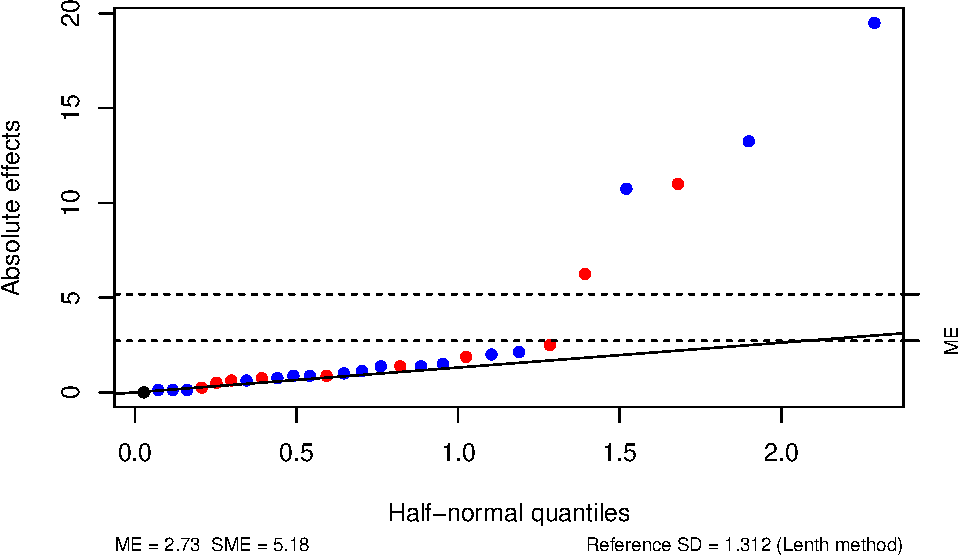
\includegraphics{bookdown_math3014-6027_files/figure-latex/block-4-lenth-1.pdf}

\hypertarget{fractional-factorial}{%
\chapter{Fractional factorial designs}\label{fractional-factorial}}

The factorial designs we studied in Chapters \ref{factorial} and \ref{factorial} can involve a large number of treatments, for even a moderate number of factors (Table \ref{tab:size-of-factorial}).

\begin{Shaded}
\begin{Highlighting}[]
\NormalTok{size }\OtherTok{\textless{}{-}} \FunctionTok{data.frame}\NormalTok{(}\DecValTok{1}\SpecialCharTok{:}\DecValTok{15}\NormalTok{, }\DecValTok{2}\SpecialCharTok{\^{}}\NormalTok{(}\DecValTok{1}\SpecialCharTok{:}\DecValTok{15}\NormalTok{))}
\NormalTok{knitr}\SpecialCharTok{::}\FunctionTok{kable}\NormalTok{(size, }\AttributeTok{col.names =} \FunctionTok{c}\NormalTok{(}\StringTok{"No. factors"}\NormalTok{, }\StringTok{"No. of trts"}\NormalTok{), }\AttributeTok{caption =} \StringTok{"Number of treatments in a $2\^{}f$ factorial designs for different numbers, $f$, of factors."}\NormalTok{)}
\end{Highlighting}
\end{Shaded}

\begin{table}

\caption{\label{tab:size-of-factorial}Number of treatments in a $2^f$ factorial designs for different numbers, $f$, of factors.}
\centering
\begin{tabular}[t]{r|r}
\hline
No. factors & No. of trts\\
\hline
1 & 2\\
\hline
2 & 4\\
\hline
3 & 8\\
\hline
4 & 16\\
\hline
5 & 32\\
\hline
6 & 64\\
\hline
7 & 128\\
\hline
8 & 256\\
\hline
9 & 512\\
\hline
10 & 1024\\
\hline
11 & 2048\\
\hline
12 & 4096\\
\hline
13 & 8192\\
\hline
14 & 16384\\
\hline
15 & 32768\\
\hline
\end{tabular}
\end{table}

For larger numbers of factors, resource constraints may mean it is not possible to run an experiment using all \(2^f\) treatments. Also, many degrees of freedom in these experiments are used to estimate high-order interactions. For example, in a \(2^5\) experiment, 16 degrees of freedom are used to estimate three-factor and higher interactions, half the size of the experiment. The principles of effect hierarchy and sparsity (Section \ref{fact-principles}) suggest this is probably wasteful.

We can select smaller experiments by using a subset, or \textbf{fraction} of the treatments of size \(2^{f-q}\):

\begin{enumerate}
\def\labelenumi{\alph{enumi}.}
\item
  divide the treatments in subsets by confounding \(q\) factorial effects (and their products), as in blocking;
\item
  only use \textbf{one} of the subsets in the experiment.
\end{enumerate}

\begin{example}
\protect\hypertarget{exm:spring-experiment}{}\label{exm:spring-experiment}

Spring experiment \citep[ch.~5]{WH2009}

Consider an industrial experiment to investigate the effect of \(f=5\) factors on the unloaded height of a spring produced using a heat treatment. The five factors are described in Table \ref{tab:spring-factors}.

\begin{Shaded}
\begin{Highlighting}[]
\NormalTok{factor.name }\OtherTok{\textless{}{-}} \FunctionTok{c}\NormalTok{(}\StringTok{"Quench temperature (F)"}\NormalTok{, }\StringTok{"Heat temperature (F)"}\NormalTok{, }\StringTok{"Heating time (s)"}\NormalTok{, }
                 \StringTok{"Transfer time (s)"}\NormalTok{, }\StringTok{"Hold{-}down time (s)"}\NormalTok{)}
\NormalTok{low.level }\OtherTok{\textless{}{-}} \FunctionTok{c}\NormalTok{(}\StringTok{"130{-}150"}\NormalTok{, }\DecValTok{1840}\NormalTok{, }\DecValTok{23}\NormalTok{, }\DecValTok{10}\NormalTok{, }\DecValTok{2}\NormalTok{)}
\NormalTok{high.level }\OtherTok{\textless{}{-}} \FunctionTok{c}\NormalTok{(}\StringTok{"150{-}170"}\NormalTok{, }\DecValTok{1880}\NormalTok{, }\DecValTok{25}\NormalTok{, }\DecValTok{12}\NormalTok{, }\DecValTok{3}\NormalTok{)}
\NormalTok{spring.factors }\OtherTok{\textless{}{-}} \FunctionTok{data.frame}\NormalTok{(}\AttributeTok{factor =}\NormalTok{ factor.name, }\AttributeTok{low =}\NormalTok{ low.level, }\AttributeTok{high =}\NormalTok{ high.level)}
\FunctionTok{row.names}\NormalTok{(spring.factors) }\OtherTok{\textless{}{-}}\NormalTok{ LETTERS[}\DecValTok{1}\SpecialCharTok{:}\DecValTok{5}\NormalTok{]}
\NormalTok{knitr}\SpecialCharTok{::}\FunctionTok{kable}\NormalTok{(spring.factors, }\AttributeTok{col.names =} \FunctionTok{c}\NormalTok{(}\StringTok{"Factor"}\NormalTok{, }\StringTok{"Low level"}\NormalTok{, }\StringTok{"High level"}\NormalTok{), }
             \AttributeTok{align =} \FunctionTok{c}\NormalTok{(}\StringTok{"l"}\NormalTok{, }\StringTok{"r"}\NormalTok{, }\StringTok{"r"}\NormalTok{), }\AttributeTok{caption =} \StringTok{"Spring experiment: factors and levels"}\NormalTok{)}
\end{Highlighting}
\end{Shaded}

\begin{table}

\caption{\label{tab:spring-factors}Spring experiment: factors and levels}
\centering
\begin{tabular}[t]{l|l|r|r}
\hline
  & Factor & Low level & High level\\
\hline
A & Quench temperature (F) & 130-150 & 150-170\\
\hline
B & Heat temperature (F) & 1840 & 1880\\
\hline
C & Heating time (s) & 23 & 25\\
\hline
D & Transfer time (s) & 10 & 12\\
\hline
E & Hold-down time (s) & 2 & 3\\
\hline
\end{tabular}
\end{table}

Enough experimental units were available to perform \(n=16\) runs, which is one-half of the total number of treatments. We refer to this type of design as a \textbf{one-half fractional replicate} of the full factorial design, or a \textbf{\(2^{5-1}\) fractional factorial design}\footnote{If we only run one-half of the treatments from a \(2^5\) design, the design contains \(\frac{2^5}{2} = 2^{5-1}\) treatments}.

The design was constructed by confounding \(q=1\) factorial effects with blocks, the interaction \(BCDE\) was chosen, and running just one of the two resulting subsets, see Table \ref{tab:spring-data} where \texttt{FrF2} is used to generate the design.

\begin{Shaded}
\begin{Highlighting}[]
\NormalTok{spring }\OtherTok{\textless{}{-}}\NormalTok{ FrF2}\SpecialCharTok{::}\FunctionTok{FrF2}\NormalTok{(}\AttributeTok{nruns =} \DecValTok{16}\NormalTok{, }\AttributeTok{nfactors =} \DecValTok{5}\NormalTok{, }\AttributeTok{generators =} \StringTok{"BCD"}\NormalTok{, }\AttributeTok{randomize =}\NormalTok{ F)}
\NormalTok{spring}\SpecialCharTok{$}\NormalTok{height }\OtherTok{\textless{}{-}} \FunctionTok{c}\NormalTok{(}\FloatTok{7.54}\NormalTok{, }\FloatTok{7.20}\NormalTok{, }\FloatTok{7.69}\NormalTok{, }\FloatTok{7.63}\NormalTok{, }\FloatTok{7.94}\NormalTok{, }\FloatTok{7.40}\NormalTok{, }\FloatTok{7.95}\NormalTok{, }\FloatTok{7.62}\NormalTok{, }\FloatTok{7.52}\NormalTok{, }\FloatTok{7.52}\NormalTok{, }
                   \FloatTok{7.63}\NormalTok{, }\FloatTok{7.65}\NormalTok{, }\FloatTok{7.79}\NormalTok{, }\FloatTok{7.29}\NormalTok{, }\FloatTok{8.07}\NormalTok{, }\FloatTok{7.73}\NormalTok{)}
\NormalTok{knitr}\SpecialCharTok{::}\FunctionTok{kable}\NormalTok{(spring, }\AttributeTok{caption =} \StringTok{"Spring experiment: 16 run design."}\NormalTok{, }\AttributeTok{align =} \FunctionTok{rep}\NormalTok{(}\StringTok{"r"}\NormalTok{, }\DecValTok{6}\NormalTok{))}
\end{Highlighting}
\end{Shaded}

\begin{table}

\caption{\label{tab:spring-data}Spring experiment: 16 run design.}
\centering
\begin{tabular}[t]{r|r|r|r|r|r}
\hline
A & B & C & D & E & height\\
\hline
-1 & -1 & -1 & -1 & -1 & 7.54\\
\hline
1 & -1 & -1 & -1 & -1 & 7.20\\
\hline
-1 & 1 & -1 & -1 & 1 & 7.69\\
\hline
1 & 1 & -1 & -1 & 1 & 7.63\\
\hline
-1 & -1 & 1 & -1 & 1 & 7.94\\
\hline
1 & -1 & 1 & -1 & 1 & 7.40\\
\hline
-1 & 1 & 1 & -1 & -1 & 7.95\\
\hline
1 & 1 & 1 & -1 & -1 & 7.62\\
\hline
-1 & -1 & -1 & 1 & 1 & 7.52\\
\hline
1 & -1 & -1 & 1 & 1 & 7.52\\
\hline
-1 & 1 & -1 & 1 & -1 & 7.63\\
\hline
1 & 1 & -1 & 1 & -1 & 7.65\\
\hline
-1 & -1 & 1 & 1 & -1 & 7.79\\
\hline
1 & -1 & 1 & 1 & -1 & 7.29\\
\hline
-1 & 1 & 1 & 1 & 1 & 8.07\\
\hline
1 & 1 & 1 & 1 & 1 & 7.73\\
\hline
\end{tabular}
\end{table}

Clearly, using a subset of the treatments, we will no longer be able to estimate all the factorial effects (we have insufficient degrees of freedom). We have confounded the interaction \(BCDE\), and hence clearly the contrast coefficients for this effect will be constant in our design. We say the interaction \(BCDE\) is \textbf{aliased} with the mean, and we write this as \(I = BCDE\). This expression is called the \textbf{defining relation}, as knowledge of which factorial effects are aliased with the mean completely define the fractional factorial.

\begin{Shaded}
\begin{Highlighting}[]
\NormalTok{fac\_to\_numeric }\OtherTok{\textless{}{-}} \ControlFlowTok{function}\NormalTok{(x) }\FunctionTok{as.numeric}\NormalTok{(}\FunctionTok{as.character}\NormalTok{(x))}
\NormalTok{BCDE }\OtherTok{\textless{}{-}} \FunctionTok{fac\_to\_numeric}\NormalTok{(spring}\SpecialCharTok{$}\NormalTok{B) }\SpecialCharTok{*} \FunctionTok{fac\_to\_numeric}\NormalTok{(spring}\SpecialCharTok{$}\NormalTok{C) }\SpecialCharTok{*} 
  \FunctionTok{fac\_to\_numeric}\NormalTok{(spring}\SpecialCharTok{$}\NormalTok{D) }\SpecialCharTok{*} \FunctionTok{fac\_to\_numeric}\NormalTok{(spring}\SpecialCharTok{$}\NormalTok{E) }
\NormalTok{BCDE}
\end{Highlighting}
\end{Shaded}

\begin{verbatim}
##  [1] 1 1 1 1 1 1 1 1 1 1 1 1 1 1 1 1
\end{verbatim}

This removes one factorial effect from consideration, but we are still short on degrees of freedom. What are the other consequences of using a fractional factorial design?

As the contrast coefficients for the interaction \(BCDE\) are constant, the contrast coefficients for any pairs of factorial effects whose (hadamard) product form \(BCDE\) will be equal. For example, the contrast coefficient vectors for interactions \(BC\) and \(DE\) will be equal, as will the vectors for the main effect \(B\) and the interaction \(CDE\), and so on.

\begin{Shaded}
\begin{Highlighting}[]
\NormalTok{BC }\OtherTok{\textless{}{-}} \FunctionTok{fac\_to\_numeric}\NormalTok{(spring}\SpecialCharTok{$}\NormalTok{B) }\SpecialCharTok{*} \FunctionTok{fac\_to\_numeric}\NormalTok{(spring}\SpecialCharTok{$}\NormalTok{C)}
\NormalTok{DE }\OtherTok{\textless{}{-}} \FunctionTok{fac\_to\_numeric}\NormalTok{(spring}\SpecialCharTok{$}\NormalTok{D) }\SpecialCharTok{*} \FunctionTok{fac\_to\_numeric}\NormalTok{(spring}\SpecialCharTok{$}\NormalTok{E)}
\NormalTok{BC}
\NormalTok{DE}
\FunctionTok{all.equal}\NormalTok{(BC, DE)}
\end{Highlighting}
\end{Shaded}

\begin{verbatim}
##  [1]  1  1 -1 -1 -1 -1  1  1  1  1 -1 -1 -1 -1  1  1
##  [1]  1  1 -1 -1 -1 -1  1  1  1  1 -1 -1 -1 -1  1  1
## [1] TRUE
\end{verbatim}

\begin{Shaded}
\begin{Highlighting}[]
\NormalTok{B }\OtherTok{\textless{}{-}} \FunctionTok{fac\_to\_numeric}\NormalTok{(spring}\SpecialCharTok{$}\NormalTok{B)}
\NormalTok{CDE }\OtherTok{\textless{}{-}} \FunctionTok{fac\_to\_numeric}\NormalTok{(spring}\SpecialCharTok{$}\NormalTok{C) }\SpecialCharTok{*} \FunctionTok{fac\_to\_numeric}\NormalTok{(spring}\SpecialCharTok{$}\NormalTok{D) }\SpecialCharTok{*} \FunctionTok{fac\_to\_numeric}\NormalTok{(spring}\SpecialCharTok{$}\NormalTok{E)}
\NormalTok{B}
\NormalTok{CDE}
\FunctionTok{all.equal}\NormalTok{(B, CDE)}
\end{Highlighting}
\end{Shaded}

\begin{verbatim}
##  [1] -1 -1  1  1 -1 -1  1  1 -1 -1  1  1 -1 -1  1  1
##  [1] -1 -1  1  1 -1 -1  1  1 -1 -1  1  1 -1 -1  1  1
## [1] TRUE
\end{verbatim}

We say these factorial effects are \textbf{aliased}. From the defining relation, we can derive the complete \textbf{aliasing scheme} for a fractional factorial design. For the example,

\begin{align}
I & = BCDE \\
A & = ABCDE \\
B & = CDE \\
C & = BDE \\
D & = BCE \\
E & = BCD \\
AB & = ACDE \\
AC & = ABDE \\
AD & = ABCE \\
AE & = ABCD \\
BC & = DE \\
BD & = CE \\
BE & = CD \\
ABC & = ADE \\
ABD & = ACE \\
ABE & = ACD \\
\end{align}

The aliasing scheme contains \(2^{f-q} = 2^{5-1} = 16\) ``strings'', each one containing \(2^q = 2^1 = 2\) ``words''. The design is not capable to distinguishing between factorial effects in the same alias string.

We can also generate this information using the \texttt{aliases} function from \texttt{FrF2}.

\begin{Shaded}
\begin{Highlighting}[]
\NormalTok{spring.lm }\OtherTok{\textless{}{-}} \FunctionTok{lm}\NormalTok{(height }\SpecialCharTok{\textasciitilde{}}\NormalTok{ (.)}\SpecialCharTok{\^{}}\DecValTok{5}\NormalTok{, }\AttributeTok{data =}\NormalTok{ spring)}
\NormalTok{FrF2}\SpecialCharTok{::}\FunctionTok{aliases}\NormalTok{(spring.lm)}
\end{Highlighting}
\end{Shaded}

\begin{verbatim}
##               
##  A = A:B:C:D:E
##  B = C:D:E    
##  C = B:D:E    
##  D = B:C:E    
##  E = B:C:D    
##  A:B = A:C:D:E
##  A:C = A:B:D:E
##  A:D = A:B:C:E
##  A:E = A:B:C:D
##  B:C = D:E    
##  B:D = C:E    
##  B:E = C:D    
##  A:B:C = A:D:E
##  A:B:D = A:C:E
##  A:B:E = A:C:D
\end{verbatim}

\end{example}

\begin{definition}
\protect\hypertarget{def:regular-fraction}{}\label{def:regular-fraction}

A \textbf{regular \(2^{f-q}\)fractional factorial design} is constructed by aliasing \(2^q-1\) factorial effects with the mean; \(q\) of these effects can be chosen independently, the others are formed via the hadamard product of the contrast coefficients for the \(q\) effects,

\end{definition}

How do we chose the factorial effects to alias with the mean? As with blocking, we tend to choose higher-order effects, taking care when \(q>1\) not to inadvertently alias together lower-order effects (see later examples).

For Example \ref{exm:spring-experiment}, a slightly unusual defining relation was chosen. It would be more common to use \(I = ABCDE\), leading to the aliasing scheme:

\begin{align}
I & = ABCDE \\
A & = BCDE \\
B & = ACDE \\
C & = ABDE \\
D & = ABCE \\
E & = ABCD \\
AB & = CDE \\
AC & = BDE \\
AD & = BCE \\
AE & = BCD \\
BC & = ADE \\
BD & = ACE \\
BE & = ACD \\
CD & = ABE \\
CE & = ABD \\
DE & = ABC \\
\end{align}

This defining relation results in main effects being aliased with four-factor interactions and, perhaps more importantly, no pairs of two-factor interactions aliased together. The original design from Example \ref{Spring-experiment} might be used if factor \(A\) and its interactions were a priori thought likely to be important (two-factor interactions involving factor \(A\) are aliased with four-factor interactions).

\hypertarget{estimability-and-aliasing}{%
\section{Estimability and aliasing}\label{estimability-and-aliasing}}

Any factorial effect in an alias string is only estimable \textbf{if all other effects in that string are assumed zero}\footnote{Except for the defining relation, where no effects are estimable}. Wd can study this further by introducing the \textbf{alias matrix}.

\begin{definition}
\protect\hypertarget{def:alias-matrix}{}\label{def:alias-matrix}

Assume a linear data generating model

\[
\boldsymbol{y}= X_1\boldsymbol{\beta}_1 + X_2\boldsymbol{\beta}_2 + \boldsymbol{\varepsilon}\,,
\]
where \(\boldsymbol{y}\) is an \(n\)-vector of responses, \(X_1\) and \(X_2\) are \(n\times p_1\) and \(n\times p_2\) model matrices, respectively, with \(\boldsymbol{\beta}_1\) and \(\boldsymbol{\beta}_2\) corresponding \(p_1\)- and \(p_2\)-vectors of parameters and random errors \(\varepsilon ~ N(\boldsymbol{0}, I_n\sigma^2)\).

If the submodel

\[
\boldsymbol{y}= X_1\boldsymbol{\beta}_1 + \boldsymbol{\varepsilon}\,,
\]
is fitted to the response data, then \(\hat{\boldsymbol{\beta}}_1 = (X_1^{\mathrm{T}}X_1)^{-1}X_1^{\mathrm{T}}\boldsymbol{y}\), and
\begin{align*}
E(\hat{\boldsymbol{\beta}}_1) & = \boldsymbol{\beta}_1 + (X_1^{\mathrm{T}}X_1)^{-1}X_1^{\mathrm{T}}X_2\boldsymbol{\beta}_2 \\
& = \boldsymbol{\beta}_1 + A\boldsymbol{\beta}_2\,,
\end{align*}
where \(A = (X_1^{\mathrm{T}}X_1)^{-1}X_1^{\mathrm{T}}X_2\) is the \textbf{alias} matrix.

\end{definition}

We also introduce an alternative definition of estimability.

\begin{definition}
\protect\hypertarget{def:alt-estimability}{}\label{def:alt-estimability}

A linear combination of parameters \(\boldsymbol{c}^{\mathrm{T}}\boldsymbol{\theta}\) is estimable if and only if there exists a linear combination of the responses \(\boldsymbol{a}^{\mathrm{T}}\boldsymbol{y}\) such that

\[
E(\boldsymbol{a}^{\mathrm{T}}\boldsymbol{y}) = c^{\mathrm{T}}\boldsymbol{\theta}\,.
\]

\end{definition}

Now assume that using a two-level fractional factorial design, we will estimate one factorial effect (equivalently, the corresponding regression coefficient) from each alias string. Then the \(A\) matrix will have entries 0, -1 or +1, depending on the defining relation of the fraction. Each regression parameter will be biased by the parameters corresponding to other factorial effects in the alias string. Hence, by Definition @ref\{def:alt-estimability\}, each factorial effect is only estimable under the assumption that all other factorial effects in the alias string are zero.

For Example \ref{exm:spring-experiment} we can generate the alias matrix using the \texttt{alias} function.

\begin{Shaded}
\begin{Highlighting}[]
\FunctionTok{t}\NormalTok{(}\FunctionTok{alias}\NormalTok{(spring.lm)}\SpecialCharTok{$}\NormalTok{Complete)}
\end{Highlighting}
\end{Shaded}

\begin{verbatim}
##             A1:C1:D1 A1:C1:E1 A1:D1:E1 B1:C1:D1 B1:C1:E1 B1:D1:E1 C1:D1:E1
## (Intercept) 0        0        0        0        0        0        0       
## A1          0        0        0        0        0        0        0       
## B1          0        0        0        0        0        0        1       
## C1          0        0        0        0        0        1        0       
## D1          0        0        0        0        1        0        0       
## E1          0        0        0        1        0        0        0       
## A1:B1       0        0        0        0        0        0        0       
## A1:C1       0        0        0        0        0        0        0       
## A1:D1       0        0        0        0        0        0        0       
## A1:E1       0        0        0        0        0        0        0       
## B1:C1       0        0        0        0        0        0        0       
## B1:D1       0        0        0        0        0        0        0       
## B1:E1       0        0        0        0        0        0        0       
## A1:B1:C1    0        0        1        0        0        0        0       
## A1:B1:D1    0        1        0        0        0        0        0       
## A1:B1:E1    1        0        0        0        0        0        0       
##             A1:B1:C1:D1 A1:B1:C1:E1 A1:B1:D1:E1 A1:C1:D1:E1 B1:C1:D1:E1
## (Intercept) 0           0           0           0           1          
## A1          0           0           0           0           0          
## B1          0           0           0           0           0          
## C1          0           0           0           0           0          
## D1          0           0           0           0           0          
## E1          0           0           0           0           0          
## A1:B1       0           0           0           1           0          
## A1:C1       0           0           1           0           0          
## A1:D1       0           1           0           0           0          
## A1:E1       1           0           0           0           0          
## B1:C1       0           0           0           0           0          
## B1:D1       0           0           0           0           0          
## B1:E1       0           0           0           0           0          
## A1:B1:C1    0           0           0           0           0          
## A1:B1:D1    0           0           0           0           0          
## A1:B1:E1    0           0           0           0           0          
##             A1:B1:C1:D1:E1 C1:D1 C1:E1 D1:E1
## (Intercept) 0              0     0     0    
## A1          1              0     0     0    
## B1          0              0     0     0    
## C1          0              0     0     0    
## D1          0              0     0     0    
## E1          0              0     0     0    
## A1:B1       0              0     0     0    
## A1:C1       0              0     0     0    
## A1:D1       0              0     0     0    
## A1:E1       0              0     0     0    
## B1:C1       0              0     0     1    
## B1:D1       0              0     1     0    
## B1:E1       0              1     0     0    
## A1:B1:C1    0              0     0     0    
## A1:B1:D1    0              0     0     0    
## A1:B1:E1    0              0     0     0
\end{verbatim}

  \bibliography{math3014-6027.bib,packages.bib}

\end{document}
